% $Header: /home/vedranm/bitbucket/beamer/solutions/conference-talks/conference-ornate-20min.en.tex,v 90e850259b8b 2007/01/28 20:48:30 tantau $

\documentclass{beamer}

% This file is a solution template for:

% - Talk at a conference/colloquium.
% - Talk length is about 20min.
% - Style is ornate.



% Copyright 2004 by Till Tantau <tantau@users.sourceforge.net>.
%
% In principle, this file can be redistributed and/or modified under
% the terms of the GNU Public License, version 2.
%
% However, this file is supposed to be a template to be modified
% for your own needs. For this reason, if you use this file as a
% template and not specifically distribute it as part of a another
% package/program, I grant the extra permission to freely copy and
% modify this file as you see fit and even to delete this copyright
% notice. 


\mode<presentation>
{
  \usetheme{Warsaw}
  \setbeamertemplate{headline}{}

  % or ...

  \setbeamercovered{transparent}
  % or whatever (possibly just delete it)
  \setbeamertemplate{footline}[frame number]

}


\usepackage[english]{babel}
% or whatever

\usepackage[utf8]{inputenc}
% or whatever

\usepackage{times}
\usepackage[T1]{fontenc}
% Or whatever. Note that the encoding and the font should match. If T1
% does not look nice, try deleting the line with the fontenc.

\usepackage{graphicx}
\usepackage{hyperref}
\usepackage{lastpage}
\usepackage{Sweave}
\usepackage{verbatim}

\title[Course Overheads] % (optional, use only with long paper titles)
{STAD29 / STA1007}
\subtitle
{Statistics for the Life and Social Sciences}

\author % (optional, use only with lots of authors)
{Ken Butler}
% - Give the names in the same order as the appear in the paper.
% - Use the \inst{?} command only if the authors have different
%   affiliation.

%\institute[testing] % (optional, but mostly needed)
%{
%  \inst{1}%
%  Department of Computer and Mathematical Sciences\\
%  University of Toronto Scarborough
%}
%% - Use the \inst command only if there are several affiliations.
% - Keep it simple, no one is interested in your street address.

\date[Winter 2013] % (optional, should be abbreviation of conference name)
{Winter semester 2013}
% - Either use conference name or its abbreviation.
% - Not really informative to the audience, more for people (including
%   yourself) who are reading the slides online

%\subject{Theoretical Computer Science}
% This is only inserted into the PDF information catalog. Can be left
% out. 



% If you have a file called "university-logo-filename.xxx", where xxx
% is a graphic format that can be processed by latex or pdflatex,
% resp., then you can add a logo as follows:

% \pgfdeclareimage[height=0.5cm]{university-logo}{university-logo-filename}
% \logo{\pgfuseimage{university-logo}}



% Delete this, if you do not want the table of contents to pop up at
% the beginning of each subsection:
\AtBeginSubsection[]
{
  \begin{frame}<beamer>{Outline}
    \tableofcontents[currentsection,currentsubsection]
  \end{frame}
}


% If you wish to uncover everything in a step-wise fashion, uncomment
% the following command: 

%\beamerdefaultoverlayspecification{<+->}


\begin{document}
%\setkeys{Gin}{width=0.6\textwidth}


\begin{frame}
  \titlepage
\end{frame}

\begin{frame}{What we (might) cover}
  \tableofcontents
  % You might wish to add the option [pausesections]
\end{frame}

\section{Review of statistical inference; 2-sample t}
\frame{\sectionpage}





\begin{frame}{The statistical world}
  \begin{itemize}
  \item 
  Consists of:

  \begin{itemize}
  \item objects or people of interest to us ({\em individuals})
  \item things measured or counted on those individuals ({\em variables})
  \end{itemize}

\pause

\item About the individuals:

\begin{itemize}
\item which ones do we care about? All of them, the {\em population}.
\item which ones do we know about? The ones we happened to look at, the {\em sample}.
\end{itemize}

\pause

\item Sample is (or should be) randomly chosen from population, with no favoritism.
  \end{itemize}

\end{frame}

\begin{frame}{Sample to population: confidence interval}
  
  \begin{itemize}
  \item 
Want to know about population (parameter), but don't. Only have sample (statistic). Eg.\ population mean, only have sample mean.
\item Logic:
  \begin{itemize}
  \item {\em If} we knew about population, could figure out kinds of samples that might appear (math).
  \item In particular, can figure how far apart sample statistic and population parameter might be.
  \item Use this to construct {\em confidence interval} for population parameter: says eg.\ ``based on my sample, I think population mean between $a$ and $b$''. 
  \end{itemize}
\end{itemize}
\end{frame}

\begin{frame}[fragile]{Example of confidence interval}
  
  \begin{itemize}
  \item Take a sample of $n=10$ observations. Obtain sample mean of
    $\bar{x}=15$, and sample SD of $s=2.5$. Want 95\% confidence
    interval for population mean.
  \item For population mean \emph{with population SD unknown}: use $t$
    distribution with $n-1=9$ degrees of freedom.
  \item Obtain $t^*$ from $t$-table or as
\begin{knitrout}
\definecolor{shadecolor}{rgb}{0.969, 0.969, 0.969}\color{fgcolor}\begin{kframe}
\begin{alltt}
\hlstd{t.star}\hlkwb{=}\hlkwd{qt}\hlstd{(}\hlnum{1}\hlopt{-}\hlnum{0.05}\hlopt{/}\hlnum{2}\hlstd{,}\hlnum{9}\hlstd{) ; t.star}
\end{alltt}
\begin{verbatim}
[1] 2.262157
\end{verbatim}
\end{kframe}
\end{knitrout}
\item and thus 95\% CI for mean is this: $m=t^* s / \sqrt{n}$, then
  $\bar{x} \pm m$:
\begin{knitrout}
\definecolor{shadecolor}{rgb}{0.969, 0.969, 0.969}\color{fgcolor}\begin{kframe}
\begin{alltt}
\hlstd{m}\hlkwb{=}\hlstd{t.star}\hlopt{*}\hlnum{2.5}\hlopt{/}\hlkwd{sqrt}\hlstd{(}\hlnum{10}\hlstd{) ; m}
\end{alltt}
\begin{verbatim}
[1] 1.788392
\end{verbatim}
\begin{alltt}
\hlkwd{c}\hlstd{(}\hlnum{15}\hlopt{-}\hlstd{m,}\hlnum{15}\hlopt{+}\hlstd{m)}
\end{alltt}
\begin{verbatim}
[1] 13.21161 16.78839
\end{verbatim}
\end{kframe}
\end{knitrout}
  \end{itemize}
  
\end{frame}

\begin{frame}{Test of significance}
\begin{itemize}
\item Or: 
  \begin{itemize}
  \item 
might have theory leading to {\em null hypothesis} (eg.\ population mean is 20) and {\em alternative hypothesis} (eg.\ population mean not 20).
\item This leads to {\em test of significance} (hypothesis test): ``based on my sample, I think pop.\ mean is (is not) 20''
\item Done by choosing $\alpha$ (eg.\ 0.05), calculating {\em test statistic} and {\em P-value}. If P-value $< \alpha$, {\em reject null}: have evidence in favour of alternative.
  \end{itemize}
\item Math producing inference procedures can be difficult, but calculations (with software) and interpretations need not be.
  \end{itemize}


\end{frame}

\begin{frame}[fragile]{Example of test of significance}
  
  
  \begin{itemize}
  \item   Let's suppose we are trying to prove that a population mean is not
  equal to 17 (alternative hypothesis), against a null that the mean
  is 17 after all. Use $\alpha=0.05$.
\item Use same data as before: $n=10, \bar{x}=15, s=2.5$.
\item Calculate test statistic $t=(\bar{x}-\mu_0)/(s/\sqrt{n})$, where
  $\mu_0$ is the population mean given by the null hypothesis:
\begin{knitrout}
\definecolor{shadecolor}{rgb}{0.969, 0.969, 0.969}\color{fgcolor}\begin{kframe}
\begin{alltt}
\hlstd{t.stat}\hlkwb{=}\hlstd{(}\hlnum{15}\hlopt{-}\hlnum{17}\hlstd{)}\hlopt{/}\hlstd{(}\hlnum{2.5}\hlopt{/}\hlkwd{sqrt}\hlstd{(}\hlnum{10}\hlstd{)) ; t.stat}
\end{alltt}
\begin{verbatim}
[1] -2.529822
\end{verbatim}
\end{kframe}
\end{knitrout}
\item Get P-value by looking along 9 df row of $t$-table, and seeing
  where \texttt{t.tstat}, or its absolute value, comes. Or get P-value
  directly from R. \emph{left} tail here, since
  \texttt{t.stat} $<0$; also $\times 2$ for
  two-sided test:
\begin{knitrout}
\definecolor{shadecolor}{rgb}{0.969, 0.969, 0.969}\color{fgcolor}\begin{kframe}
\begin{alltt}
\hlnum{2}\hlopt{*}\hlkwd{pt}\hlstd{(t.stat,}\hlnum{9}\hlstd{)}
\end{alltt}
\begin{verbatim}
[1] 0.03224478
\end{verbatim}
\end{kframe}
\end{knitrout}
  \end{itemize}
  
\end{frame}

\begin{frame}[fragile]{Conclusion}
  
  \begin{itemize}
  \item $\alpha=0.05$, P-value was 0.032.
  \item P-value less than $\alpha$, so \emph{reject} null hypothesis
    in favour of alternative: that is, population mean \emph{not} equal to 17.
  \item If had $\alpha=0.01$, would not have been able to reject
    null. So evidence against a mean of 17 is strong but not
    \emph{that} strong.
  \end{itemize}
\end{frame}

\begin{frame}[fragile]{Doing it in R}
  


\begin{itemize}
\item These data have right mean and SD:
\begin{knitrout}
\definecolor{shadecolor}{rgb}{0.969, 0.969, 0.969}\color{fgcolor}\begin{kframe}
\begin{alltt}
\hlstd{mydata}
\end{alltt}
\begin{verbatim}
 [1] 18.99229 15.25282 11.22454 14.66774
 [5] 14.89869 14.34578 16.47864 10.89571
 [9] 17.38091 15.86289
\end{verbatim}
\end{kframe}
\end{knitrout}
\item One step with R (note everything as before):
  {\small
\begin{knitrout}
\definecolor{shadecolor}{rgb}{0.969, 0.969, 0.969}\color{fgcolor}\begin{kframe}
\begin{alltt}
\hlkwd{t.test}\hlstd{(mydata,}\hlkwc{mu}\hlstd{=}\hlnum{17}\hlstd{)}
\end{alltt}
\begin{verbatim}

	One Sample t-test

data:  mydata
t = -2.5298, df = 9, p-value = 0.03224
alternative hypothesis: true mean is not equal to 17
95 percent confidence interval:
 13.21161 16.78839
sample estimates:
mean of x 
       15 
\end{verbatim}
\end{kframe}
\end{knitrout}
}
\end{itemize}
  
\end{frame}

\begin{frame}{Exploratory data analysis}
  \begin{itemize}
  \item Sometimes don't have theory (yet), just want to see what data
    tell us.
  \item Use graphs, simple descriptive statistics, some of methods we learn.
  \item Idea: generate ideas (``hypotheses'') for future study.
  \item Cannot make clear conclusions about populations.
  \end{itemize}
\end{frame}


\begin{frame}{The Degree of Reading Power data}

  \begin{itemize}
  \item Have new method for teaching reading.
  \item Want to see if better than ``standard'' method (``research hypothesis'').
  \item Design: randomly allocate available children to ``treatment''
    (new method) or ``control'' (standard).
  \item Measure score for all children on standard reading test.
  \item Analysis: is observed difference between treatment/control score
    means big enough to be real not chance? Do 2-sample $t$-test.
  \end{itemize}

\end{frame}

\begin{frame}[fragile]{Some of the data}

\begin{verbatim}
t 43
t 53
t 57
t 49
t 56
t 33
c 42
c 33
c 46
c 37
c 43
\end{verbatim}

  \begin{itemize}
  \item 1st column label (``t'' for treatment, ``c'' for control).
  \item 2nd column response (score on reading test).
  \item Data in plain text file \verb-drp.txt-.

  \end{itemize}
  
\end{frame}


\begin{frame}[fragile]{Reading and examining data}
  
 
\begin{knitrout}
\definecolor{shadecolor}{rgb}{0.969, 0.969, 0.969}\color{fgcolor}\begin{kframe}
\begin{alltt}
\hlstd{drp}\hlkwb{=}\hlkwd{read.table}\hlstd{(}\hlstr{"drp.txt"}\hlstd{,}\hlkwc{header}\hlstd{=T)}
\hlkwd{head}\hlstd{(drp)}
\end{alltt}
\begin{verbatim}
  group score
1     t    24
2     t    61
3     t    59
4     t    46
5     t    43
6     t    44
\end{verbatim}
\end{kframe}
\end{knitrout}

\begin{itemize}
\item \texttt{read.table} gets data from ``space-delimited'' text
  file. \texttt{header=T} reads top line as variable names.
\item Resulting R data structure called \texttt{data.frame}, basic
  arrangement for data in R.
\item \texttt{head} looks at first few lines (default 6) of data frame.
\end{itemize}

 
\end{frame}

\begin{frame}[fragile]{Visual comparison of groups}
  
  \begin{itemize}
  \item My favourite tool: \textbf{boxplot}:
    
\begin{knitrout}
\definecolor{shadecolor}{rgb}{0.969, 0.969, 0.969}\color{fgcolor}\begin{kframe}
\begin{alltt}
\hlstd{gbox}\hlkwb{=}\hlkwd{ggplot}\hlstd{(drp,}\hlkwd{aes}\hlstd{(}\hlkwc{x}\hlstd{=group,}\hlkwc{y}\hlstd{=score))}\hlopt{+}\hlkwd{geom_boxplot}\hlstd{()}
\hlstd{gbox}
\end{alltt}
\end{kframe}
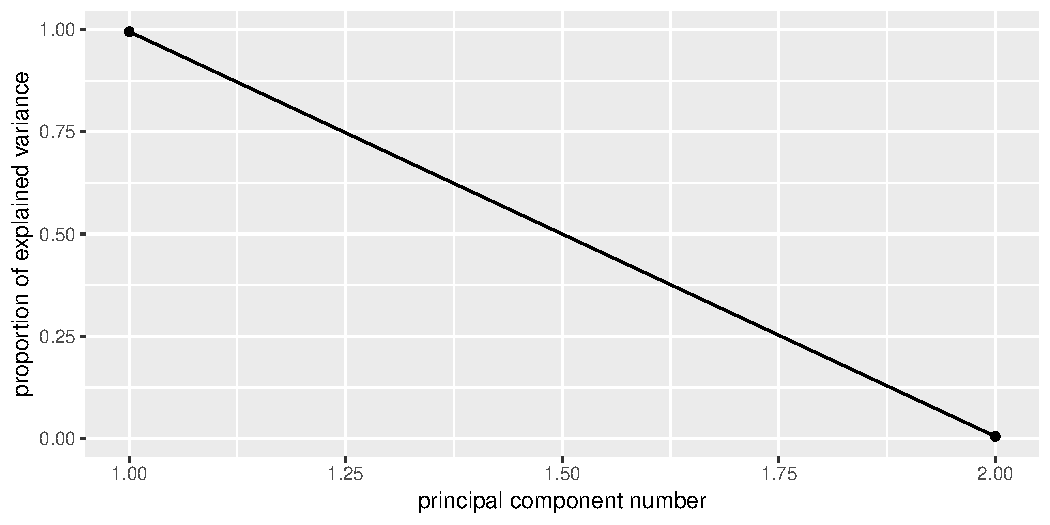
\includegraphics[width=\maxwidth]{figure/unnamed-chunk-8-1} 

\end{knitrout}
    

  \end{itemize}
  
\end{frame}



\begin{frame}[fragile]{Comments and setup}
  
  \begin{itemize}
  \item Mean reading score for treatment group is higher
  \item but a lot of variability.
  \item Is that difference real/reproducible?
  \item Do \emph{two-sample $t$-test}.
  \item \textbf{P-value} tells you whether difference in samples
    likely to persist in population
  \item Small P-value (less than 0.05) means ``yes, it's real''
  \item Confidence interval says how far apart means might be.
  \end{itemize}
  
\end{frame}

\begin{frame}[fragile]{Two-sample $t$}

{\small

 
\begin{knitrout}
\definecolor{shadecolor}{rgb}{0.969, 0.969, 0.969}\color{fgcolor}\begin{kframe}
\begin{alltt}
\hlkwd{with}\hlstd{(drp,}\hlkwd{t.test}\hlstd{(score}\hlopt{~}\hlstd{group))}
\end{alltt}
\begin{verbatim}

	Welch Two Sample t-test

data:  score by group
t = -2.3109, df = 37.855, p-value =
0.02638
alternative hypothesis: true difference in means is not equal to 0
95 percent confidence interval:
 -18.67588  -1.23302
sample estimates:
mean in group c mean in group t 
       41.52174        51.47619 
\end{verbatim}
\end{kframe}
\end{knitrout}

}

\begin{itemize}
\item P-value 0.026 says means really are different
\item CI says difference between 1 and 19 points in favour of new
  reading program.
\item R puts groups in alphabetical order (\texttt{c} before \texttt{t}).
\end{itemize}

\end{frame}


\begin{frame}{Comments}

  \begin{itemize}
  \item New reading program really helps!
  \item 2 possible $t$ procedures:
    \begin{itemize}
    \item Pooled: assumes 2 population variances/SDs are same
    \item Welch/Satterthwaite: does not, but only approximation.
    \end{itemize}
  \item R does Welch by default. If willing to assume equal variances,
    add \texttt{var.equal=T} to \texttt{t.test}.
  \end{itemize}
  
\end{frame}

%\usepackage[utf8]{inputenc}

\section{Review of (multiple) regression}
\frame{\sectionpage}




\begin{frame}{Regression}

  \begin{itemize}
  \item Use regression when one variable is an outcome ({\em response}, $y$).
  \item See if/how response depends on other variable(s), {\em explanatory}, $x_1, x_2,\ldots$.
  \item Can have {\em one} or {\em more than one} explanatory variable, but always one response.
  \item Assumes a {\em straight-line} relationship between response and explanatory.
  \item Ask: 
    \begin{itemize}
    \item {\em is there} a relationship between $y$ and $x$'s, and if so, which ones?
    \item what does the relationship look like?
    \end{itemize}

  \end{itemize}
  
\end{frame}

\begin{frame}[fragile]{A regression with one $x$}

13 children, measure average total sleep time (ATST, mins) and age (years) for each. See if ATST depends on age. Data in \verb-sleep.txt-, ATST then age. Read in data:

 
\begin{knitrout}
\definecolor{shadecolor}{rgb}{0.969, 0.969, 0.969}\color{fgcolor}\begin{kframe}
\begin{alltt}
\hlstd{sleep}\hlkwb{=}\hlkwd{read.table}\hlstd{(}\hlstr{"sleep.txt"}\hlstd{,}\hlkwc{header}\hlstd{=T)}
\hlkwd{head}\hlstd{(sleep)}
\end{alltt}
\begin{verbatim}
    atst  age
1 586.00  4.4
2 461.75 14.0
3 491.10 10.1
4 565.00  6.7
5 462.00 11.5
6 532.10  9.6
\end{verbatim}
\end{kframe}
\end{knitrout}

and make scatter plot of ATST (response) vs.\ age (explanatory) using
code overleaf:

 


\end{frame}




\begin{frame}[fragile]{The scatterplot}
   
\begin{knitrout}
\definecolor{shadecolor}{rgb}{0.969, 0.969, 0.969}\color{fgcolor}\begin{kframe}
\begin{alltt}
\hlkwd{ggplot}\hlstd{(sleep,}\hlkwd{aes}\hlstd{(}\hlkwc{x}\hlstd{=age,}\hlkwc{y}\hlstd{=atst))}\hlopt{+}\hlkwd{geom_point}\hlstd{()}
\end{alltt}
\end{kframe}
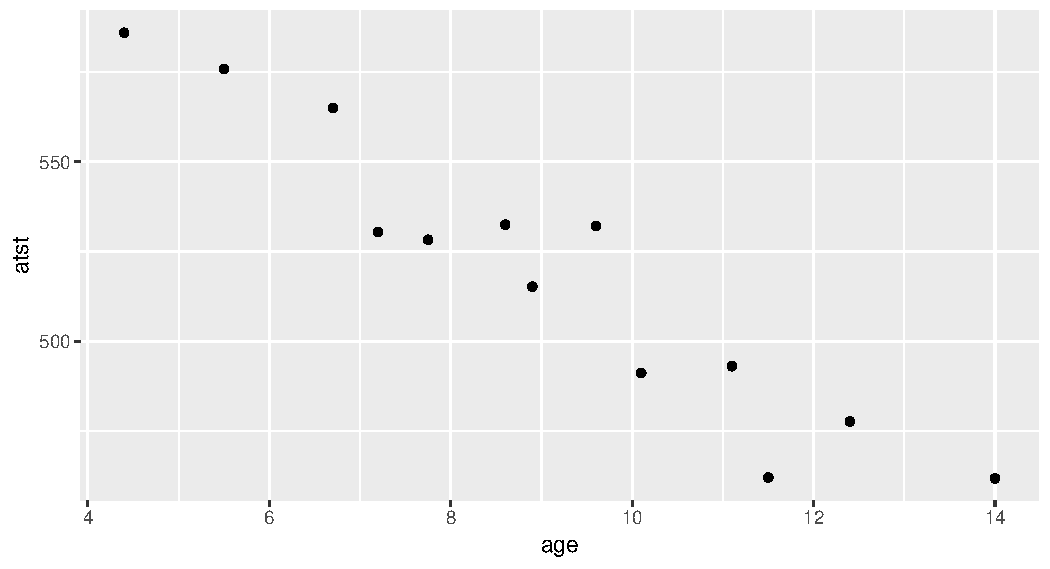
\includegraphics[width=\maxwidth]{figure/suggo-1} 

\end{knitrout}
  
  
%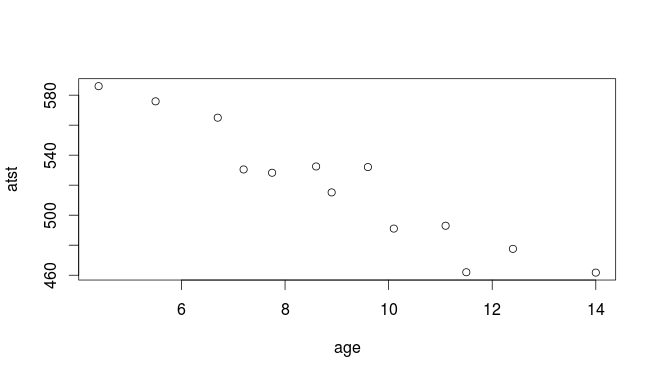
\includegraphics[width=\textwidth]{sleep-times}

\end{frame}

\begin{frame}[fragile]{Correlation}
  
  \begin{itemize}
  \item Measures how well a straight line fits the data:
 
\begin{knitrout}
\definecolor{shadecolor}{rgb}{0.969, 0.969, 0.969}\color{fgcolor}\begin{kframe}
\begin{alltt}
\hlkwd{with}\hlstd{(sleep,}\hlkwd{cor}\hlstd{(atst,age))}
\end{alltt}
\begin{verbatim}
[1] -0.9515469
\end{verbatim}
\end{kframe}
\end{knitrout}

\item $1$ is perfect upward trend, $-1$ is perfect downward trend, 0
  is no trend.
\item This one close to perfect downward trend.
\item Can do correlations of whole data frame:
 
\begin{knitrout}
\definecolor{shadecolor}{rgb}{0.969, 0.969, 0.969}\color{fgcolor}\begin{kframe}
\begin{alltt}
\hlkwd{cor}\hlstd{(sleep)}
\end{alltt}
\begin{verbatim}
           atst        age
atst  1.0000000 -0.9515469
age  -0.9515469  1.0000000
\end{verbatim}
\end{kframe}
\end{knitrout}
\item Correlations of all possible pairs of variables.  
    
  \end{itemize}
  
\end{frame}


\begin{frame}[fragile]{Lowess curve}
  
  \begin{itemize}
  \item Sometimes nice to guide the eye: is the trend straight, or not?

  \item Idea: \emph{lowess curve}. ``Locally weighted least squares'',
    not affected by outliers, not constrained to be linear.
  \item Lowess is a \emph{guide}: even if straight line appropriate,
    may wiggle/bend a little. Looking for \emph{serious} problems with
    linearity. 
  \item Add lowess curve to plot using \texttt{geom\_smooth}:
 
    
  \end{itemize}
  
\end{frame}

\begin{frame}[fragile]{Plot with lowess curve}
  

\begin{knitrout}
\definecolor{shadecolor}{rgb}{0.969, 0.969, 0.969}\color{fgcolor}\begin{kframe}
\begin{alltt}
\hlkwd{ggplot}\hlstd{(sleep,}\hlkwd{aes}\hlstd{(}\hlkwc{x}\hlstd{=age,}\hlkwc{y}\hlstd{=atst))}\hlopt{+}\hlkwd{geom_point}\hlstd{()}\hlopt{+}
  \hlkwd{geom_smooth}\hlstd{()}
\end{alltt}


{\ttfamily\noindent\itshape\color{messagecolor}{`geom\_smooth()` using method = 'loess'}}\end{kframe}
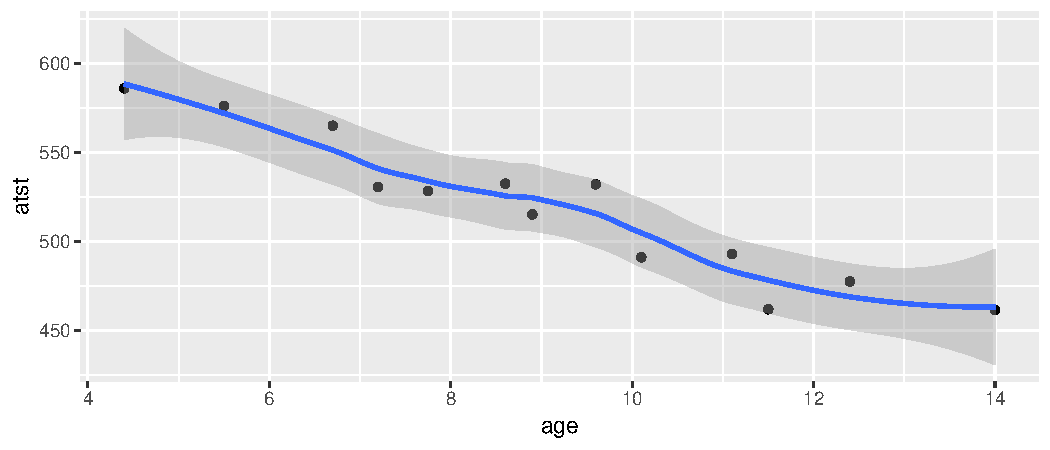
\includegraphics[width=\maxwidth]{figure/icko-1} 

\end{knitrout}

  
  
\end{frame}


\begin{frame}[fragile]{The regression}

Scatterplot shows no obvious curve, and a pretty clear downward trend. So we can run the regression:

{\scriptsize
 
\begin{knitrout}
\definecolor{shadecolor}{rgb}{0.969, 0.969, 0.969}\color{fgcolor}\begin{kframe}
\begin{alltt}
\hlstd{sleep.1}\hlkwb{=}\hlkwd{lm}\hlstd{(atst}\hlopt{~}\hlstd{age,}\hlkwc{data}\hlstd{=sleep) ;} \hlkwd{summary}\hlstd{(sleep.1)}
\end{alltt}
\begin{verbatim}

Call:
lm(formula = atst ~ age, data = sleep)

Residuals:
    Min      1Q  Median      3Q     Max 
-23.011  -9.365   2.372   6.770  20.411 

Coefficients:
            Estimate Std. Error t value Pr(>|t|)    
(Intercept)  646.483     12.918   50.05 2.49e-14 ***
age          -14.041      1.368  -10.26 5.70e-07 ***
---
Signif. codes:  
0 '***' 0.001 '**' 0.01 '*' 0.05 '.' 0.1 ' ' 1

Residual standard error: 13.15 on 11 degrees of freedom
Multiple R-squared:  0.9054,	Adjusted R-squared:  0.8968 
F-statistic: 105.3 on 1 and 11 DF,  p-value: 5.7e-07
\end{verbatim}
\end{kframe}
\end{knitrout}
}


\end{frame}

\begin{frame}{Conclusions}

    \begin{itemize}
  \item The relationship appears to be a straight line, with a downward trend.
  \item $F$-tests for model as a whole and $t$-test for slope (same)
    both confirm this (P-value $5.7\times 10^{-7}=0.00000057$).
  \item Slope is $-14$, so a 1-year increase in age goes with a 14-minute decrease in ATST on average.
  \item R-squared is correlation squared (when one $x$ anyway),
    between 0 and 1 (1 good, 0 bad).
  \item Here R-squared is 0.9054, pleasantly high.
  \end{itemize}
  
\end{frame}

% for week 2:
% 
% regression and multiple regression
% 
% including univariate + tests
% ci, pi and influential points
% multiple, re-interpretation of tests, correlated x's
% residuals and plotting
% 

% next: ci and pi with children aged 10 and 3
% then: maybe diagnostics

\begin{frame}{CI for mean response and prediction intervals}

Once useful regression exists, use it for prediction:


\begin{itemize}
\item To get a single number for prediction at a given $x$, substitute into regression equation, eg.\ age 10: predicted ATST is $646.48-14.04(10)=506$ minutes.
\item To express uncertainty of this prediction:
  \begin{itemize}
  \item {\em CI for mean response} expresses uncertainty about mean ATST for all children aged 10, based on data.
  \item {\em Prediction interval} expresses uncertainty about predicted ATST for a new child aged 10 whose ATST not known. More uncertain.
  \end{itemize}
\item Also do above for a child aged 5.
\end{itemize}
\end{frame}

\begin{frame}[fragile]{Intervals}
\begin{itemize}
\item Make new data frame with these values for \texttt{age}
\item Feed into \texttt{predict}:
  
{\small  
 
\begin{knitrout}
\definecolor{shadecolor}{rgb}{0.969, 0.969, 0.969}\color{fgcolor}\begin{kframe}
\begin{alltt}
\hlstd{my.age}\hlkwb{=}\hlkwd{c}\hlstd{(}\hlnum{10}\hlstd{,}\hlnum{5}\hlstd{)}
\hlstd{ages.new}\hlkwb{=}\hlkwd{data.frame}\hlstd{(}\hlkwc{age}\hlstd{=my.age)}
\hlstd{ages.new}
\end{alltt}
\begin{verbatim}
  age
1  10
2   5
\end{verbatim}
\begin{alltt}
\hlstd{pc}\hlkwb{=}\hlkwd{predict}\hlstd{(sleep.1,ages.new,}\hlkwc{interval}\hlstd{=}\hlstr{"c"}\hlstd{)}
\hlstd{pp}\hlkwb{=}\hlkwd{predict}\hlstd{(sleep.1,ages.new,}\hlkwc{interval}\hlstd{=}\hlstr{"p"}\hlstd{)}
\end{alltt}
\end{kframe}
\end{knitrout}
}

  
\end{itemize}

\end{frame}

\begin{frame}[fragile]{The intervals}
  
Confidence intervals for mean response:

 
\begin{knitrout}
\definecolor{shadecolor}{rgb}{0.969, 0.969, 0.969}\color{fgcolor}\begin{kframe}
\begin{alltt}
\hlkwd{cbind}\hlstd{(ages.new,pc)}
\end{alltt}
\begin{verbatim}
  age      fit      lwr      upr
1  10 506.0729 497.5574 514.5883
2   5 576.2781 561.6578 590.8984
\end{verbatim}
\end{kframe}
\end{knitrout}

Prediction intervals for new response:

 
\begin{knitrout}
\definecolor{shadecolor}{rgb}{0.969, 0.969, 0.969}\color{fgcolor}\begin{kframe}
\begin{alltt}
\hlkwd{cbind}\hlstd{(ages.new,pp)}
\end{alltt}
\begin{verbatim}
  age      fit      lwr      upr
1  10 506.0729 475.8982 536.2475
2   5 576.2781 543.8474 608.7088
\end{verbatim}
\end{kframe}
\end{knitrout}


  
\end{frame}


\begin{frame}[fragile]{Comments}

\begin{itemize}
\item Age 10 closer to centre of data, so intervals are both narrower than those for age 5.
\item Prediction intervals bigger than CI for mean (additional uncertainty).
\end{itemize}

\end{frame}


\begin{frame}[fragile]{That grey envelope}
  
\begin{knitrout}
\definecolor{shadecolor}{rgb}{0.969, 0.969, 0.969}\color{fgcolor}\begin{kframe}
\begin{alltt}
\hlstd{h5}\hlkwb{=}\hlkwd{ggplot}\hlstd{(sleep,}\hlkwd{aes}\hlstd{(}\hlkwc{x}\hlstd{=age,}\hlkwc{y}\hlstd{=atst))}\hlopt{+}\hlkwd{geom_point}\hlstd{()}\hlopt{+}
  \hlkwd{geom_smooth}\hlstd{(}\hlkwc{method}\hlstd{=}\hlstr{"lm"}\hlstd{)}\hlopt{+}
  \hlkwd{scale_y_continuous}\hlstd{(}\hlkwc{breaks}\hlstd{=}\hlkwd{seq}\hlstd{(}\hlnum{420}\hlstd{,}\hlnum{600}\hlstd{,}\hlnum{20}\hlstd{)) ; h5}
\end{alltt}
\end{kframe}
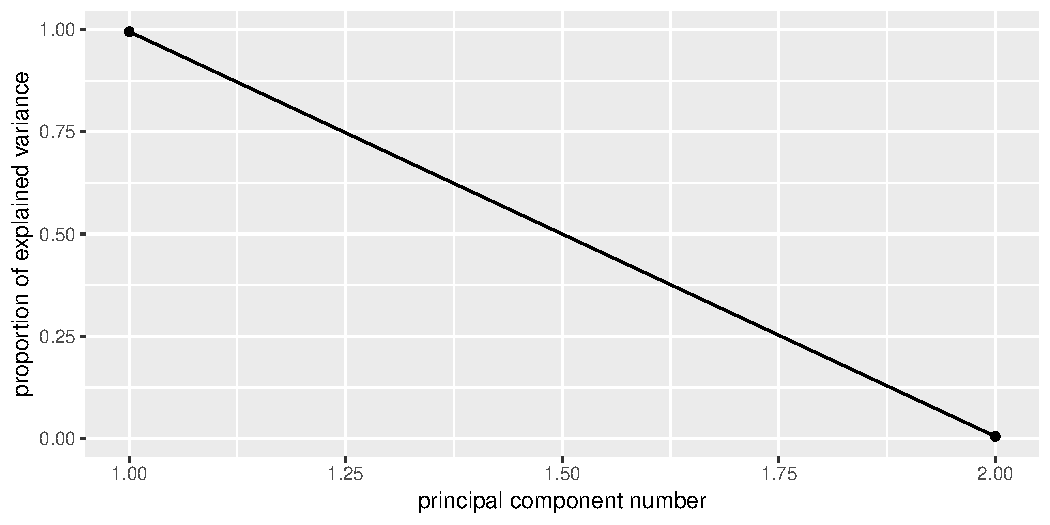
\includegraphics[width=\maxwidth]{figure/unnamed-chunk-8-1} 

\end{knitrout}

Marks confidence interval for mean for all $x$.
  
\end{frame}

\begin{frame}[fragile]{Diagnostics}
How to tell whether a straight-line regression is appropriate?

\vspace{3ex}

\begin{itemize}
\item Before: check scatterplot for straight trend.
\item After: plot {\em residuals} (observed minus predicted response) against predicted values. Aim: a plot with no pattern.
\end{itemize}

\vspace{3ex}


\end{frame}

\begin{frame}[fragile]{Output}

 
\begin{knitrout}
\definecolor{shadecolor}{rgb}{0.969, 0.969, 0.969}\color{fgcolor}\begin{kframe}
\begin{alltt}
\hlkwd{ggplot}\hlstd{(sleep.1,}\hlkwd{aes}\hlstd{(}\hlkwc{x}\hlstd{=.fitted,}\hlkwc{y}\hlstd{=.resid))}\hlopt{+}\hlkwd{geom_point}\hlstd{()}
\end{alltt}
\end{kframe}
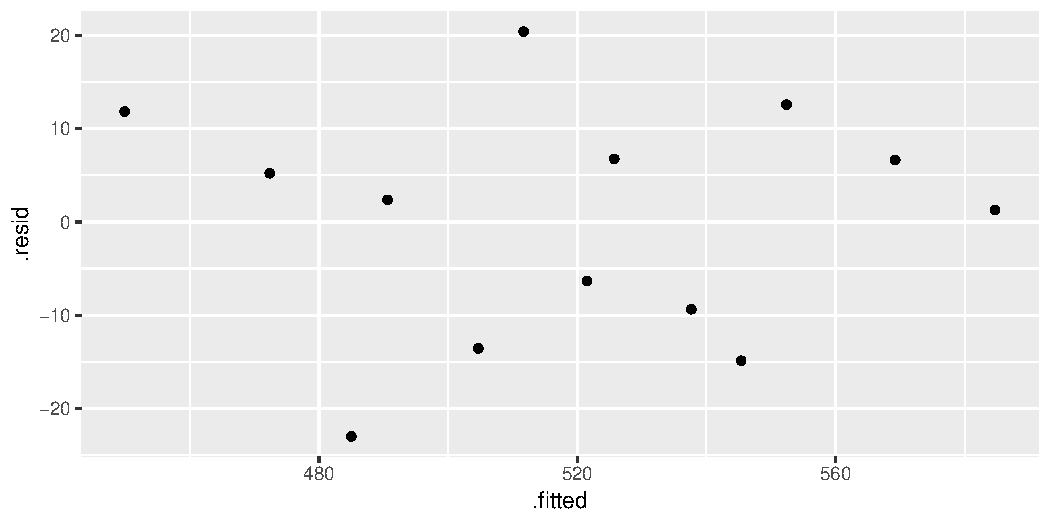
\includegraphics[width=\maxwidth]{figure/akjhkadjfhjahnkkk-1} 

\end{knitrout}
  
%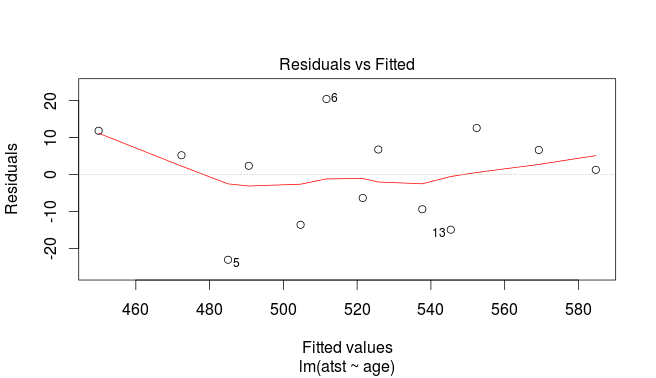
\includegraphics[width=4in]{sleep-resid}

Not much pattern here (is residual predictable from predicted? No). Good, indicating regression appropriate.
  
\end{frame}


\begin{frame}[fragile]{An inappropriate regression}

Scatterplot of different data:  
  
{\footnotesize
 
\begin{knitrout}
\definecolor{shadecolor}{rgb}{0.969, 0.969, 0.969}\color{fgcolor}\begin{kframe}
\begin{alltt}
\hlstd{curvy}\hlkwb{=}\hlkwd{read.table}\hlstd{(}\hlstr{"curvy.txt"}\hlstd{,}\hlkwc{header}\hlstd{=T)}
\hlkwd{ggplot}\hlstd{(curvy,}\hlkwd{aes}\hlstd{(}\hlkwc{x}\hlstd{=xx,}\hlkwc{y}\hlstd{=yy))}\hlopt{+}\hlkwd{geom_point}\hlstd{()}
\end{alltt}
\end{kframe}
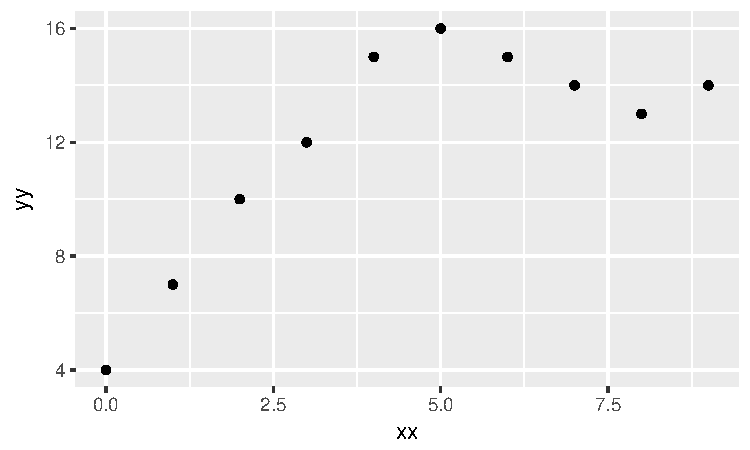
\includegraphics[width=\maxwidth]{figure/curvy-1} 

\end{knitrout}
}  
  

%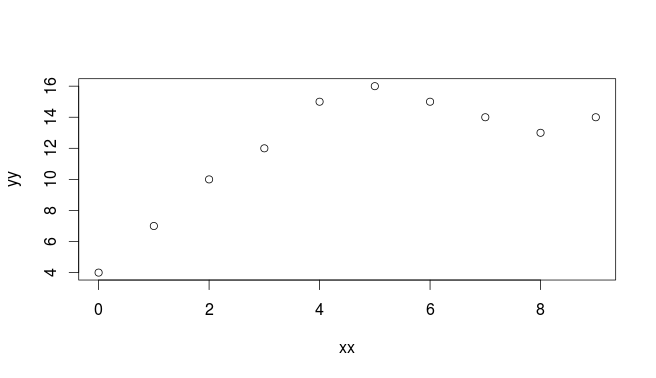
\includegraphics[width=4in]{curvy-scatter}


\end{frame}

\begin{frame}[fragile]{Regression line, anyway}

{\footnotesize
 
\begin{knitrout}
\definecolor{shadecolor}{rgb}{0.969, 0.969, 0.969}\color{fgcolor}\begin{kframe}
\begin{alltt}
\hlstd{curvy.1}\hlkwb{=}\hlkwd{lm}\hlstd{(yy}\hlopt{~}\hlstd{xx,}\hlkwc{data}\hlstd{=curvy) ;} \hlkwd{summary}\hlstd{(curvy.1)}
\end{alltt}
\begin{verbatim}

Call:
lm(formula = yy ~ xx, data = curvy)

Residuals:
   Min     1Q Median     3Q    Max 
-3.582 -2.204  0.000  1.514  3.509 

Coefficients:
            Estimate Std. Error t value Pr(>|t|)   
(Intercept)   7.5818     1.5616   4.855  0.00126 **
xx            0.9818     0.2925   3.356  0.00998 **
---
Signif. codes:  
0 '***' 0.001 '**' 0.01 '*' 0.05 '.' 0.1 ' ' 1

Residual standard error: 2.657 on 8 degrees of freedom
Multiple R-squared:  0.5848,	Adjusted R-squared:  0.5329 
F-statistic: 11.27 on 1 and 8 DF,  p-value: 0.009984
\end{verbatim}
\end{kframe}
\end{knitrout}
}
  
\end{frame}



\begin{frame}[fragile]{Residual plot}

 
\begin{knitrout}
\definecolor{shadecolor}{rgb}{0.969, 0.969, 0.969}\color{fgcolor}\begin{kframe}
\begin{alltt}
\hlkwd{ggplot}\hlstd{(curvy.1,}\hlkwd{aes}\hlstd{(}\hlkwc{x}\hlstd{=.fitted,}\hlkwc{y}\hlstd{=.resid))}\hlopt{+}\hlkwd{geom_point}\hlstd{()}
\end{alltt}
\end{kframe}
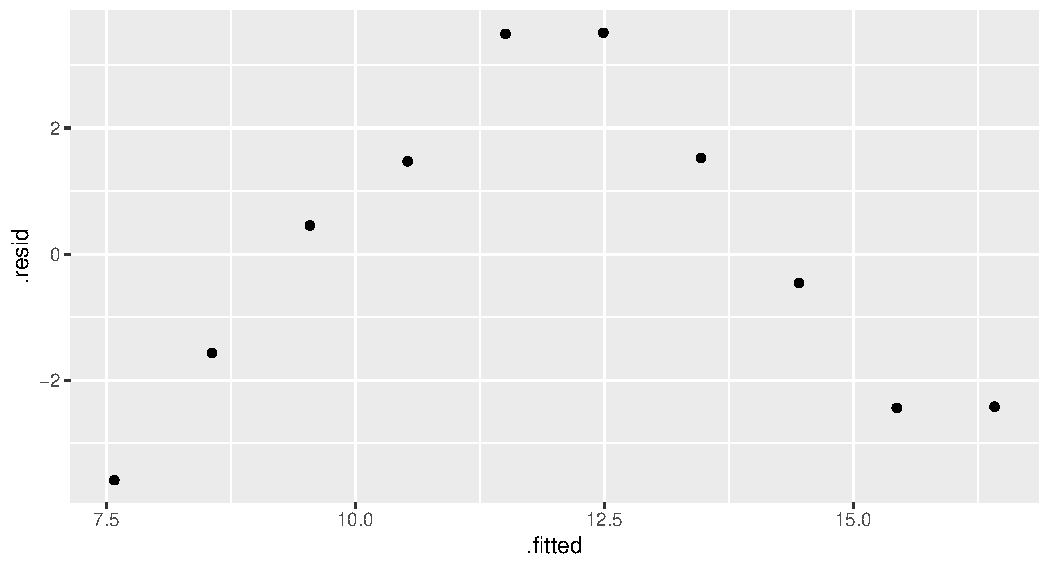
\includegraphics[width=\maxwidth]{figure/altoadige-1} 

\end{knitrout}
  
  
%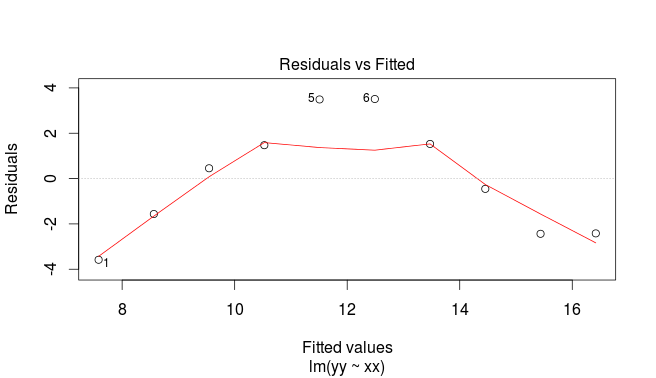
\includegraphics[width=4in]{curvy-residual}

  
\end{frame}

\begin{frame}[fragile]{No good: fixing it up}

  \begin{itemize}
  \item Residual plot has {\em curve}: middle residuals positive, high and low ones negative. Bad.
  \item Fitting a curve would be better. Try this:
  



\begin{knitrout}
\definecolor{shadecolor}{rgb}{0.969, 0.969, 0.969}\color{fgcolor}\begin{kframe}
\begin{alltt}
\hlstd{curvy.2}\hlkwb{=}\hlkwd{lm}\hlstd{(yy}\hlopt{~}\hlstd{xx}\hlopt{+}\hlkwd{I}\hlstd{(xx}\hlopt{^}\hlnum{2}\hlstd{),}\hlkwc{data}\hlstd{=curvy)}
\end{alltt}
\end{kframe}
\end{knitrout}



\item Adding \texttt{xx}-squared term, to allow for curve.
  \end{itemize}


\end{frame}



\begin{frame}[fragile]{Regression 2}
  
{\scriptsize
 
\begin{knitrout}
\definecolor{shadecolor}{rgb}{0.969, 0.969, 0.969}\color{fgcolor}\begin{kframe}
\begin{alltt}
\hlkwd{summary}\hlstd{(curvy.2)}
\end{alltt}
\begin{verbatim}

Call:
lm(formula = yy ~ xx + I(xx^2), data = curvy)

Residuals:
    Min      1Q  Median      3Q     Max 
-1.2091 -0.3602 -0.2364  0.8023  1.2636 

Coefficients:
            Estimate Std. Error t value Pr(>|t|)    
(Intercept)  3.90000    0.77312   5.045 0.001489 ** 
xx           3.74318    0.40006   9.357 3.31e-05 ***
I(xx^2)     -0.30682    0.04279  -7.170 0.000182 ***
---
Signif. codes:  
0 '***' 0.001 '**' 0.01 '*' 0.05 '.' 0.1 ' ' 1

Residual standard error: 0.9833 on 7 degrees of freedom
Multiple R-squared:  0.9502,	Adjusted R-squared:  0.936 
F-statistic: 66.83 on 2 and 7 DF,  p-value: 2.75e-05
\end{verbatim}
\end{kframe}
\end{knitrout}
  }
  
\end{frame}

\begin{frame}[fragile]{Comments}
  
  \begin{itemize}
  \item \texttt{xx}-squared term definitely significant (P-value
    0.000182), so need this curve to describe relationship.
  \item Adding squared term has made R-squared go up from 0.5848 to
    0.9502: great improvement.
  \item This is a definite curve!
  \end{itemize}
  
\end{frame}


\begin{frame}[fragile]{The residual plot now}

  
 
\begin{knitrout}
\definecolor{shadecolor}{rgb}{0.969, 0.969, 0.969}\color{fgcolor}\begin{kframe}
\begin{alltt}
\hlkwd{ggplot}\hlstd{(curvy.2,}\hlkwd{aes}\hlstd{(}\hlkwc{x}\hlstd{=.fitted,}\hlkwc{y}\hlstd{=.resid))}\hlopt{+}\hlkwd{geom_point}\hlstd{()}
\end{alltt}
\end{kframe}
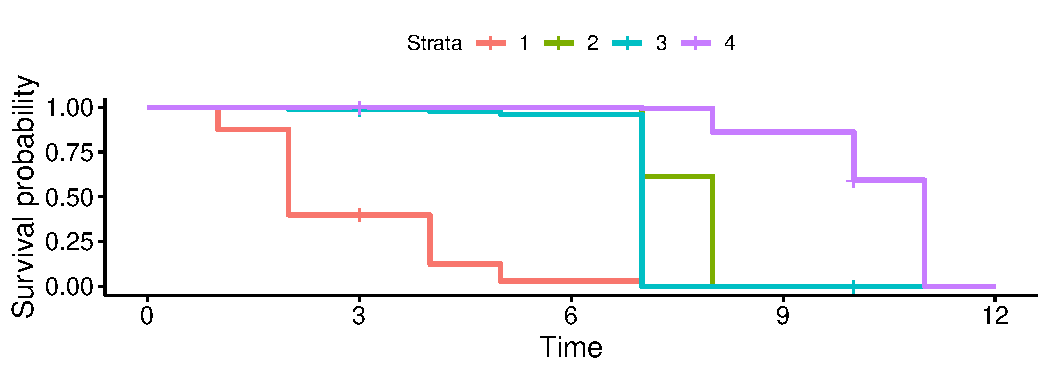
\includegraphics[width=\maxwidth]{figure/unnamed-chunk-12-1} 

\end{knitrout}

%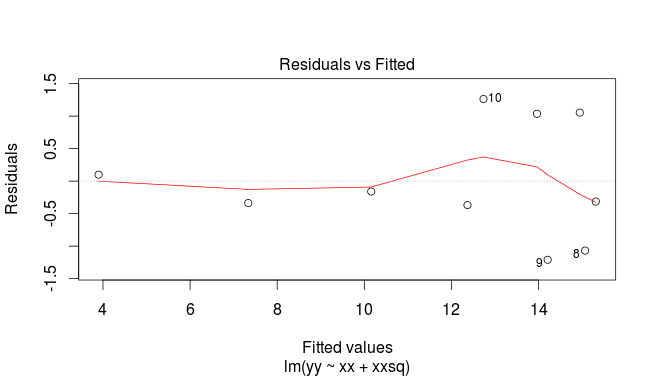
\includegraphics[width=4in]{curvy-resid2}

No problems any more.  

\end{frame}

\begin{frame}[fragile]{Another way to handle curves}
  
  \begin{itemize}
  \item Above, saw that changing $x$ (adding $x^2$) was a way of
    handling curved relationships.
  \item Another way: change $y$ (transformation).
  \item Can guess how to change $y$, or might be theory:
    \begin{itemize}
    \item example: relationship $y=ae^{bx}$ (exponential growth): 

    \item take
      logs to get $\ln y=\ln a + bx$.
    \item Taking logs has made relationship linear ($\ln y$ as response).
    \end{itemize}
  \item Or, \emph{estimate} transformation, using Box-Cox method. 
  \end{itemize}
  
\end{frame}

\begin{frame}[fragile]{Box-Cox}
  
  \begin{itemize}
  \item Install package \texttt{MASS} via
 
\begin{knitrout}
\definecolor{shadecolor}{rgb}{0.969, 0.969, 0.969}\color{fgcolor}\begin{kframe}
\begin{alltt}
\hlkwd{install.packages}\hlstd{(}\hlstr{"MASS"}\hlstd{)}
\end{alltt}
\end{kframe}
\end{knitrout}
(only need to do \emph{once})
\item Every R session you want to use something in \texttt{MASS}, type
  (no quotes)
 
\begin{knitrout}
\definecolor{shadecolor}{rgb}{0.969, 0.969, 0.969}\color{fgcolor}\begin{kframe}
\begin{alltt}
\hlkwd{library}\hlstd{(MASS)}
\end{alltt}


{\ttfamily\noindent\itshape\color{messagecolor}{\\Attaching package: 'MASS'}}

{\ttfamily\noindent\itshape\color{messagecolor}{The following object is masked from 'package:dplyr':

\ \ \ \ select}}\end{kframe}
\end{knitrout}

\end{itemize}
  
\end{frame}

\begin{frame}[fragile]{Some made-up data}
  
 
\begin{knitrout}
\definecolor{shadecolor}{rgb}{0.969, 0.969, 0.969}\color{fgcolor}\begin{kframe}
\begin{alltt}
\hlstd{madeup}\hlkwb{=}\hlkwd{read.csv}\hlstd{(}\hlstr{"madeup.csv"}\hlstd{)}
\hlstd{madeup}
\end{alltt}
\begin{verbatim}
  row x         y
1   1 0  17.92576
2   2 1  33.58480
3   3 2  82.69371
4   4 3  31.19415
5   5 4 177.07919
6   6 5 358.70001
7   7 6 469.30232
8   8 7 583.24106
\end{verbatim}
\end{kframe}
\end{knitrout}
  
Seems to be faster-than-linear growth, maybe exponential growth. Scatterplot?

 

  
\end{frame}

\begin{frame}[fragile]{The scatterplot: faster than linear growth}

  
 
\begin{knitrout}
\definecolor{shadecolor}{rgb}{0.969, 0.969, 0.969}\color{fgcolor}\begin{kframe}
\begin{alltt}
\hlkwd{ggplot}\hlstd{(madeup,}\hlkwd{aes}\hlstd{(}\hlkwc{x}\hlstd{=x,}\hlkwc{y}\hlstd{=y))}\hlopt{+}\hlkwd{geom_point}\hlstd{()}\hlopt{+}
  \hlkwd{geom_smooth}\hlstd{()}
\end{alltt}


{\ttfamily\noindent\itshape\color{messagecolor}{`geom\_smooth()` using method = 'loess'}}\end{kframe}
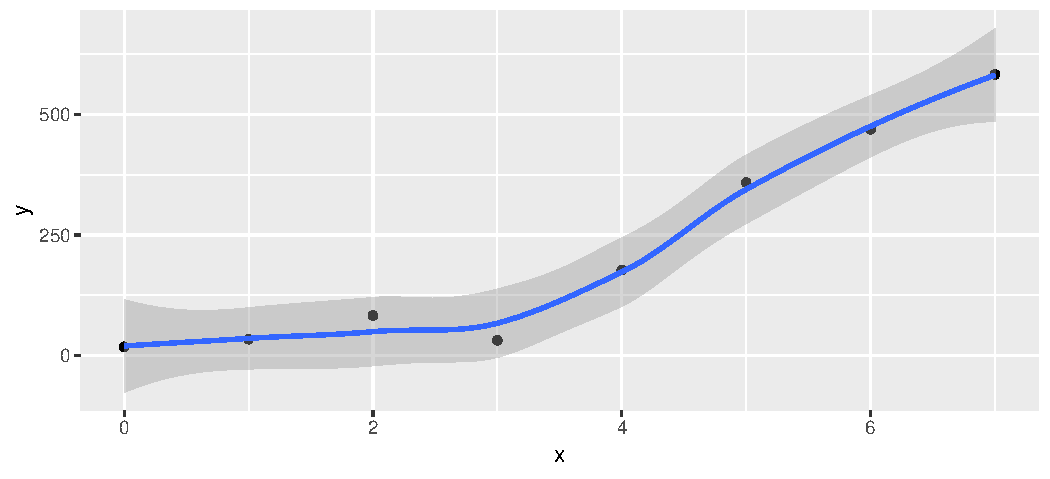
\includegraphics[width=\maxwidth]{figure/dsljhsdjlhf-1} 

\end{knitrout}

  
  
\end{frame}

\begin{frame}[fragile]{Running Box-Cox}
  
  \begin{itemize}
  \item Feed \texttt{boxcox} a model formula with a squiggle in it,
    such as you would use for \texttt{lm}.
  \item Output: a graph (next page):
 
\begin{knitrout}
\definecolor{shadecolor}{rgb}{0.969, 0.969, 0.969}\color{fgcolor}\begin{kframe}
\begin{alltt}
\hlkwd{boxcox}\hlstd{(y}\hlopt{~}\hlstd{x,}\hlkwc{data}\hlstd{=madeup)}
\end{alltt}
\end{kframe}
\end{knitrout}
    
  \end{itemize}
  
\end{frame}

\begin{frame}[fragile]{The Box-Cox output}
  
 
\begin{knitrout}
\definecolor{shadecolor}{rgb}{0.969, 0.969, 0.969}\color{fgcolor}
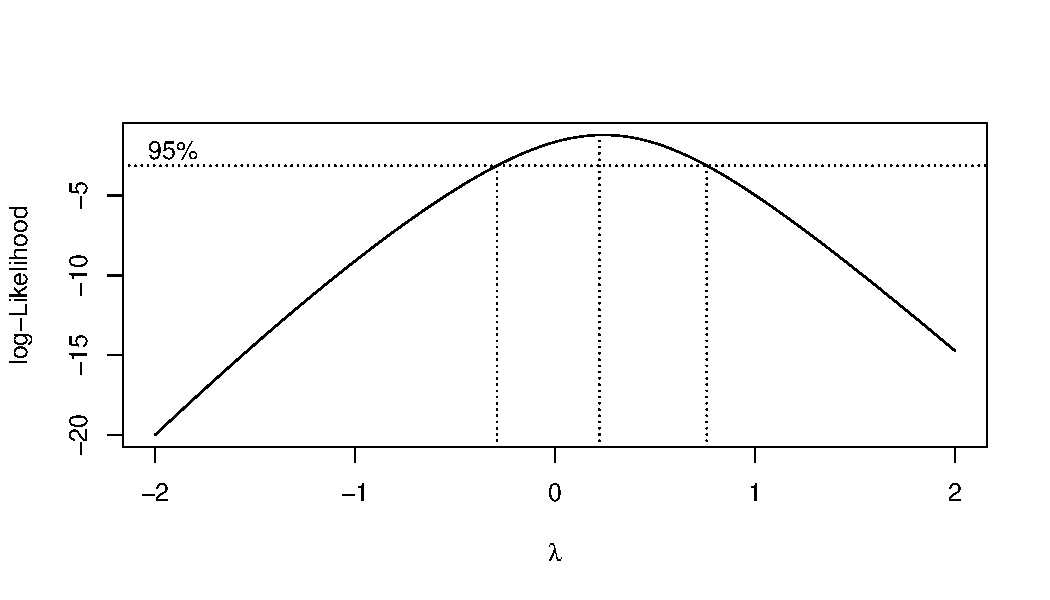
\includegraphics[width=\maxwidth]{figure/trento-1} 

\end{knitrout}
  
  
\end{frame}

\begin{frame}[fragile]{Comments}
  \begin{itemize}
  \item $\lambda$ (lambda) is the power by which you should transform
    $y$ to get the relationship straight (straighter). Power 0 is
    ``take logs''
  \item Middle dotted line marks best single value of $\lambda$ (here
    about 0.1).
  \item Outer dotted lines mark 95\% CI for $\lambda$, here $-0.3$ to
    0.7, approx. (Rather uncertain about best transformation.)
  \item Any power transformation within the CI supported by data. In
    this case, log ($\lambda=0$) and square root ($\lambda=0.5$) good,
    but no transformation ($\lambda=1$)  not.
  \item Pick a ``round-number'' value of $\lambda$ like
    $2,1,0.5,0,-0.5,-1$. Here 0 and 0.5 good values to pick. 
  \end{itemize}
\end{frame}

\begin{frame}[fragile]{Did transformation straighten things?}
  
  \begin{itemize}
  \item Calculate transformed $y$ and plot against $x$. Here try log:
 
 
\begin{knitrout}
\definecolor{shadecolor}{rgb}{0.969, 0.969, 0.969}\color{fgcolor}\begin{kframe}
\begin{alltt}
\hlstd{log.y}\hlkwb{=}\hlkwd{log}\hlstd{(madeup}\hlopt{$}\hlstd{y)}
\hlkwd{ggplot}\hlstd{(madeup,}\hlkwd{aes}\hlstd{(}\hlkwc{x}\hlstd{=x,}\hlkwc{y}\hlstd{=log.y))}\hlopt{+}\hlkwd{geom_point}\hlstd{()}\hlopt{+}
  \hlkwd{geom_smooth}\hlstd{()}
\end{alltt}


{\ttfamily\noindent\itshape\color{messagecolor}{`geom\_smooth()` using method = 'loess'}}\end{kframe}
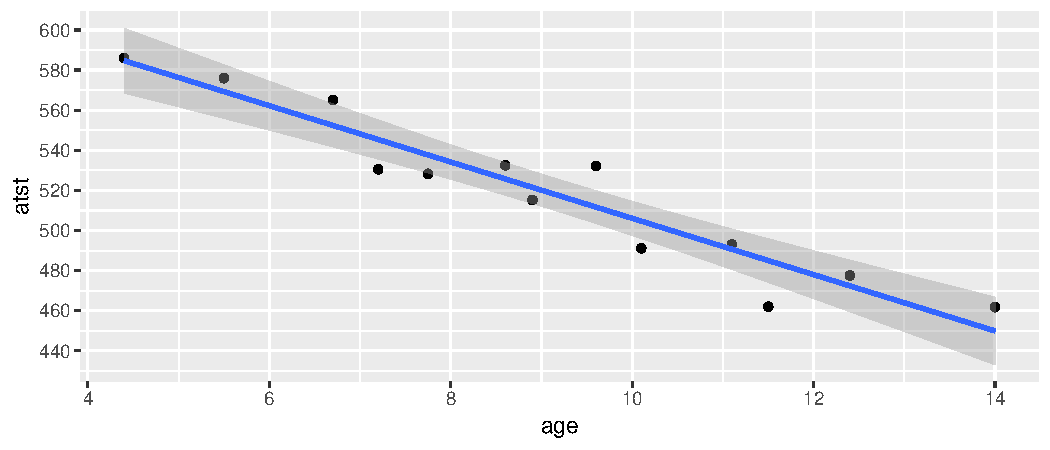
\includegraphics[width=\maxwidth]{figure/unnamed-chunk-17-1} 

\end{knitrout}

    
  \end{itemize}
  
\end{frame}

%%%%%%%%%%%%%%%%%%%%%%%%%%%%%%%%%%%%%%%%%%%%

\begin{frame}[fragile]{Multiple regression}

  \begin{itemize}
  \item What if more than one $x$? Extra issues: % regression ex from before
    \begin{itemize}
    \item Now one intercept and a slope for each $x$: how to interpret?
    \item Which $x$-variables actually help to predict $y$?

    \item Different interpretations of ``global'' $F$-test and individual $t$-tests.
    \item R-squared no longer correlation squared, but still
      interpreted as ``higher better''.
    \end{itemize}
  \item In \verb-lm- line, add extra $x$s after \verb-~-.
  \item Interpretation not so easy (and other problems that can occur).
  \end{itemize}

\end{frame}

\begin{frame}[fragile]{Multiple regression example}

Study of women and visits to health professionals, and how the number of visits might be related to other variables:

\begin{description}
\item[timedrs:] number of visits to health professionals (over course of study)
\item[phyheal:] number of physical health problems
\item[menheal:] number of mental health problems
\item[stress:] result of questionnaire about number and type of life changes
\end{description}

\verb-timedrs- response, others explanatory.

\end{frame}

\begin{frame}[fragile]{The data, fit multiple regression}

 
\begin{knitrout}
\definecolor{shadecolor}{rgb}{0.969, 0.969, 0.969}\color{fgcolor}\begin{kframe}
\begin{alltt}
\hlstd{visits}\hlkwb{=}\hlkwd{read.table}\hlstd{(}\hlstr{"regressx.txt"}\hlstd{,}\hlkwc{header}\hlstd{=T)}
\hlkwd{head}\hlstd{(visits)}
\end{alltt}
\begin{verbatim}
  subjno timedrs phyheal menheal stress
1      1       1       5       8    265
2      2       3       4       6    415
3      3       0       3       4     92
4      4      13       2       2    241
5      5      15       3       6     86
6      6       3       5       5    247
\end{verbatim}
\begin{alltt}
\hlkwd{attach}\hlstd{(visits)}
\hlstd{visits.1}\hlkwb{=}\hlkwd{lm}\hlstd{(timedrs}\hlopt{~}\hlstd{phyheal}\hlopt{+}\hlstd{menheal}\hlopt{+}\hlstd{stress)}
\end{alltt}
\end{kframe}
\end{knitrout}
  


\end{frame}

\begin{frame}[fragile]{The regression}

{\scriptsize
 
\begin{knitrout}
\definecolor{shadecolor}{rgb}{0.969, 0.969, 0.969}\color{fgcolor}\begin{kframe}
\begin{alltt}
\hlkwd{summary}\hlstd{(visits.1)}
\end{alltt}
\begin{verbatim}

Call:
lm(formula = timedrs ~ phyheal + menheal + stress)

Residuals:
    Min      1Q  Median      3Q     Max 
-14.792  -4.353  -1.815   0.902  65.886 

Coefficients:
             Estimate Std. Error t value Pr(>|t|)    
(Intercept) -3.704848   1.124195  -3.296 0.001058 ** 
phyheal      1.786948   0.221074   8.083  5.6e-15 ***
menheal     -0.009666   0.129029  -0.075 0.940318    
stress       0.013615   0.003612   3.769 0.000185 ***
---
Signif. codes:  
0 '***' 0.001 '**' 0.01 '*' 0.05 '.' 0.1 ' ' 1

Residual standard error: 9.708 on 461 degrees of freedom
Multiple R-squared:  0.2188,	Adjusted R-squared:  0.2137 
F-statistic: 43.03 on 3 and 461 DF,  p-value: < 2.2e-16
\end{verbatim}
\end{kframe}
\end{knitrout}
}  
  

\end{frame}


\begin{frame}[fragile]{The slopes}

Model as a whole strongly significant even though R-sq not very big (lots of data). At least one of the $x$'s predicts \verb-timedrs-.

\begin{footnotesize}
\begin{knitrout}
\definecolor{shadecolor}{rgb}{0.969, 0.969, 0.969}\color{fgcolor}\begin{kframe}
\begin{alltt}
\hlkwd{summary}\hlstd{(visits.1)}\hlopt{$}\hlstd{coefficients}
\end{alltt}
\begin{verbatim}
                Estimate  Std. Error     t value
(Intercept) -3.704847732 1.124195055 -3.29555598
phyheal      1.786948071 0.221073522  8.08304884
menheal     -0.009665606 0.129028610 -0.07491056
stress       0.013614518 0.003612149  3.76909138
                Pr(>|t|)
(Intercept) 1.058053e-03
phyheal     5.604170e-15
menheal     9.403184e-01
stress      1.851166e-04
\end{verbatim}
\end{kframe}
\end{knitrout}
  
\end{footnotesize}

The physical health and stress variables definitely help to predict the number of visits, but {\em with those in the model} we don't need \verb-menheal-.


However, look at prediction of \verb-timedrs- from \verb-menheal- by itself:
  
\end{frame}

\begin{frame}[fragile]{Just \texttt{menheal}}

{\footnotesize 
 
\begin{knitrout}
\definecolor{shadecolor}{rgb}{0.969, 0.969, 0.969}\color{fgcolor}\begin{kframe}
\begin{alltt}
\hlstd{visits.2}\hlkwb{=}\hlkwd{lm}\hlstd{(timedrs}\hlopt{~}\hlstd{menheal) ;} \hlkwd{summary}\hlstd{(visits.2)}
\end{alltt}
\begin{verbatim}

Call:
lm(formula = timedrs ~ menheal)

Residuals:
    Min      1Q  Median      3Q     Max 
-13.826  -5.150  -2.818   1.177  72.513 

Coefficients:
            Estimate Std. Error t value Pr(>|t|)    
(Intercept)   3.8159     0.8702   4.385 1.44e-05 ***
menheal       0.6672     0.1173   5.688 2.28e-08 ***
---
Signif. codes:  
0 '***' 0.001 '**' 0.01 '*' 0.05 '.' 0.1 ' ' 1

Residual standard error: 10.6 on 463 degrees of freedom
Multiple R-squared:  0.06532,	Adjusted R-squared:  0.0633 
F-statistic: 32.35 on 1 and 463 DF,  p-value: 2.279e-08
\end{verbatim}
\end{kframe}
\end{knitrout}
}

\end{frame}

\begin{frame}[fragile]{\texttt{menheal} by itself}

  \begin{itemize}
  \item \verb-menheal- by itself {\em does} significantly help to predict \verb-timedrs-.
  \item But the R-sq is much less (6.5\% vs.\ 22\%).
  \item So other two variables do a better job of prediction.
  \item With those variables in the regression (\texttt{phyheal} and
    \texttt{stress}), don't need \texttt{menheal} \emph{as well}.

  \end{itemize}
  


  
\end{frame}





\begin{frame}[fragile]{Investigating via correlation}
  
Leave out first column (\texttt{subjno}):
  
 
\begin{knitrout}
\definecolor{shadecolor}{rgb}{0.969, 0.969, 0.969}\color{fgcolor}\begin{kframe}
\begin{alltt}
\hlkwd{cor}\hlstd{(visits[,}\hlopt{-}\hlnum{1}\hlstd{])}
\end{alltt}
\begin{verbatim}
          timedrs   phyheal   menheal    stress
timedrs 1.0000000 0.4395293 0.2555703 0.2865951
phyheal 0.4395293 1.0000000 0.5049464 0.3055517
menheal 0.2555703 0.5049464 1.0000000 0.3697911
stress  0.2865951 0.3055517 0.3697911 1.0000000
\end{verbatim}
\end{kframe}
\end{knitrout}
  
\begin{itemize}
\item \texttt{phyheal} most strongly correlated with \texttt{timedrs}.
\item Not much to choose between other two.
\item But \texttt{menheal} has higher correlation with \texttt{phyheal},
  so not as much to \emph{add} to prediction as \texttt{stress}.
\item Goes to show things more complicated in multiple regression.

\end{itemize}

  
\end{frame}

\begin{frame}[fragile]{Residual plot (from \texttt{timedrs} on all)}
 
\begin{knitrout}
\definecolor{shadecolor}{rgb}{0.969, 0.969, 0.969}\color{fgcolor}\begin{kframe}
\begin{alltt}
\hlkwd{ggplot}\hlstd{(visits.1,}\hlkwd{aes}\hlstd{(}\hlkwc{x}\hlstd{=.fitted,}\hlkwc{y}\hlstd{=.resid))}\hlopt{+}\hlkwd{geom_point}\hlstd{()}
\end{alltt}
\end{kframe}
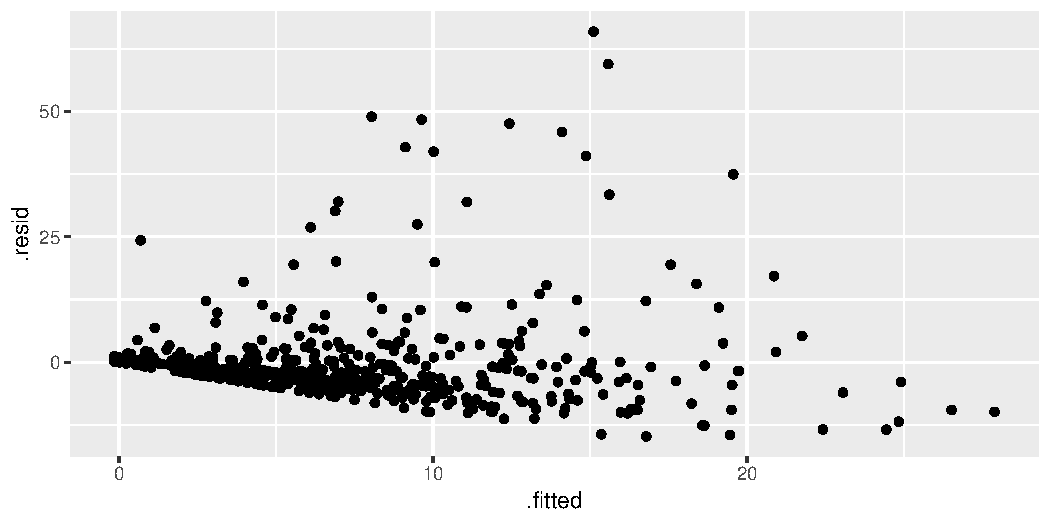
\includegraphics[width=\maxwidth]{figure/iffy8-1} 

\end{knitrout}

Apparently random. But look at all output from \texttt{plot(visits.1)}:

%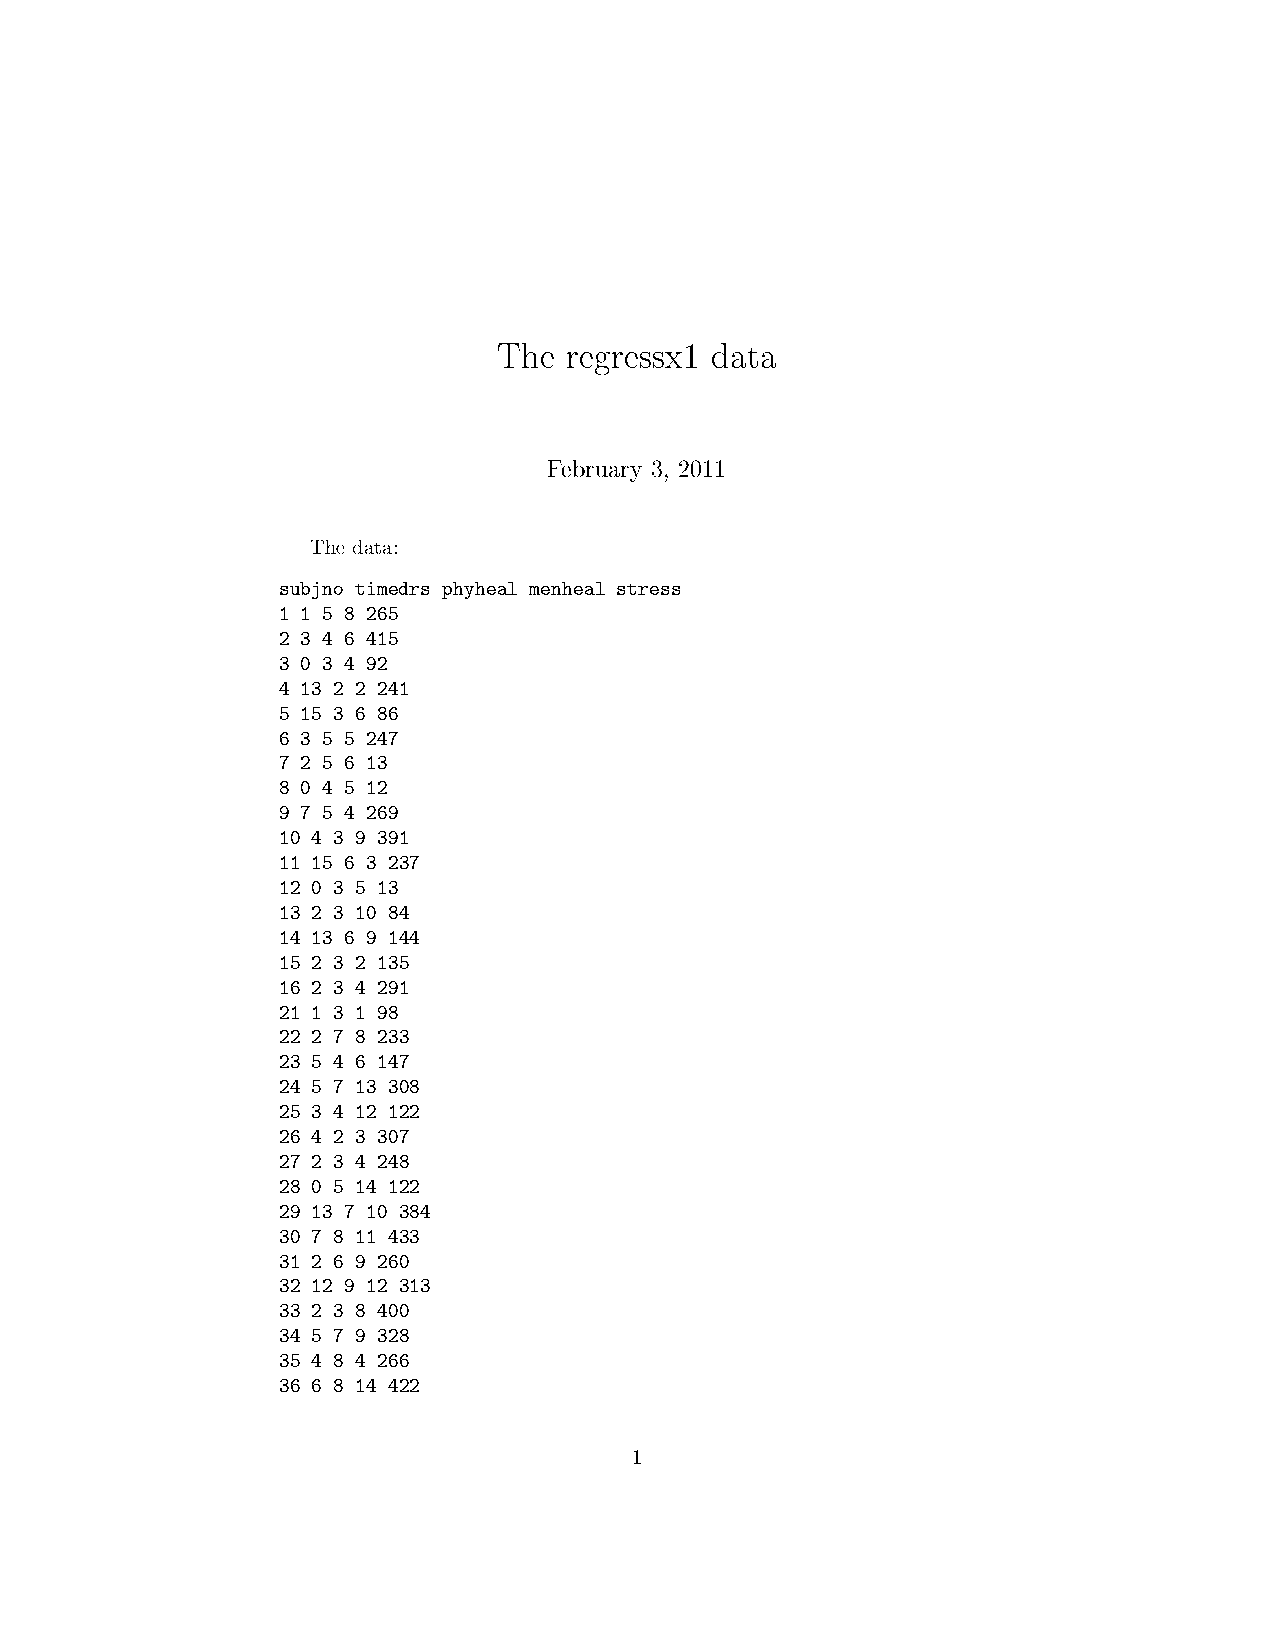
\includegraphics[width=4in]{regressx1}

\end{frame}

\begin{frame}[fragile]{Plot of regression object}
  
  
 
\begin{knitrout}
\definecolor{shadecolor}{rgb}{0.969, 0.969, 0.969}\color{fgcolor}\begin{kframe}
\begin{alltt}
\hlkwd{par}\hlstd{(}\hlkwc{mfrow}\hlstd{=}\hlkwd{c}\hlstd{(}\hlnum{2}\hlstd{,}\hlnum{2}\hlstd{)) ;} \hlkwd{plot}\hlstd{(visits.1)}
\end{alltt}
\end{kframe}
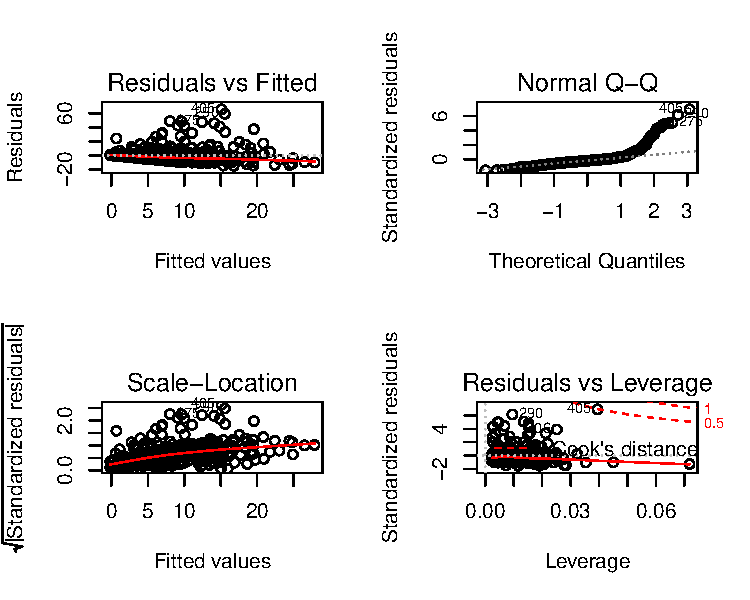
\includegraphics[width=\maxwidth]{figure/dawlish-1} 

\end{knitrout}
  
  
\end{frame}

\begin{frame}[fragile]{What are those plots?}
  
  \begin{itemize}
  \item Top left: ordinary residual plot
    \begin{itemize}
    \item no apparent pattern here
    \end{itemize}
  \item Top right: normal quantile plot of residuals
    \begin{itemize}
    \item residuals should be normally distributed
    \item should follow dotted line
    \item largest (positive) residuals are much too big
    \end{itemize}
  \item Bottom left: \emph{size} of residuals
    \begin{itemize}
    \item should stay constant
    \item here seems to be increasing: ``fan out''.
    \end{itemize}
  \item Bottom right: unusual/influential observations
    \begin{itemize}
    \item Obs at 0.07 on $x$ scale has unusual combo of $x$'s
    \item Obs 405 (top) influential over slopes.
    \end{itemize}
  \end{itemize}
  
\end{frame}


\begin{frame}[fragile]{Fixing the problems}

  \begin{itemize}
  \item Residuals not normal (skewed right), increase in size with
    fitted value.
  \item Sometimes residuals are {\em very} positive: observed a {\em lot} larger than predicted.
  \item Try {\em  transforming} response: use log or square root of response. (Note that response is {\em count}, often skewed to right.)
  \item Try regression again, with transformed response instead of
    original one.
  \item Then check residual plot to see that it is OK now.

 
\begin{knitrout}
\definecolor{shadecolor}{rgb}{0.969, 0.969, 0.969}\color{fgcolor}\begin{kframe}
\begin{alltt}
\hlstd{lgtime}\hlkwb{=}\hlkwd{log}\hlstd{(timedrs}\hlopt{+}\hlnum{1}\hlstd{)}
\hlstd{visits.3}\hlkwb{=}\hlkwd{lm}\hlstd{(lgtime}\hlopt{~}\hlstd{phyheal}\hlopt{+}\hlstd{menheal}\hlopt{+}\hlstd{stress)}
\end{alltt}
\end{kframe}
\end{knitrout}
    
\item \texttt{timedrs+1}  because some \texttt{timedrs} values 0,
  can't take log of 0.
  \end{itemize}
  
\end{frame}


\begin{frame}[fragile]{Output}

{\scriptsize
 
\begin{knitrout}
\definecolor{shadecolor}{rgb}{0.969, 0.969, 0.969}\color{fgcolor}\begin{kframe}
\begin{alltt}
\hlkwd{summary}\hlstd{(visits.3)}
\end{alltt}
\begin{verbatim}

Call:
lm(formula = lgtime ~ phyheal + menheal + stress)

Residuals:
     Min       1Q   Median       3Q      Max 
-1.95865 -0.44076 -0.02331  0.42304  2.36797 

Coefficients:
             Estimate Std. Error t value Pr(>|t|)    
(Intercept) 0.3903862  0.0882908   4.422 1.22e-05 ***
phyheal     0.2019361  0.0173624  11.631  < 2e-16 ***
menheal     0.0071442  0.0101335   0.705    0.481    
stress      0.0013158  0.0002837   4.638 4.58e-06 ***
---
Signif. codes:  
0 '***' 0.001 '**' 0.01 '*' 0.05 '.' 0.1 ' ' 1

Residual standard error: 0.7625 on 461 degrees of freedom
Multiple R-squared:  0.3682,	Adjusted R-squared:  0.3641 
F-statistic: 89.56 on 3 and 461 DF,  p-value: < 2.2e-16
\end{verbatim}
\end{kframe}
\end{knitrout}
}
 
\end{frame}

\begin{frame}[fragile]{Comments}

  \begin{itemize}
  \item Model as a whole strongly significant again 
  \item R-sq higher than before (37\% vs.\ 22\%) suggesting things more linear now
  \item Same conclusion re \verb-menheal-: can take out of regression.
  \item Should look at residual plots (next page).
  \end{itemize}
  
\end{frame}

\begin{frame}[fragile]{The residual plots}

 
\begin{knitrout}
\definecolor{shadecolor}{rgb}{0.969, 0.969, 0.969}\color{fgcolor}\begin{kframe}
\begin{alltt}
\hlkwd{par}\hlstd{(}\hlkwc{mfrow}\hlstd{=}\hlkwd{c}\hlstd{(}\hlnum{2}\hlstd{,}\hlnum{2}\hlstd{)) ;} \hlkwd{plot}\hlstd{(visits.3)}
\end{alltt}
\end{kframe}
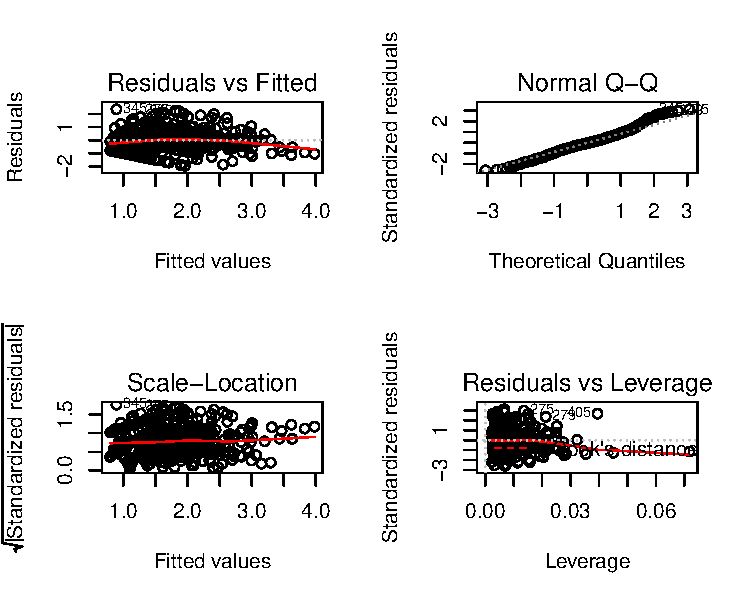
\includegraphics[width=\maxwidth]{figure/asljsakjhd-1} 

\end{knitrout}
  
  
\end{frame}

\begin{frame}[fragile]{Comments}

  
  \begin{itemize}
  \item Residuals range from about 2 to $-2$.
  \item Residuals look much more normally distributed.
  \item Size of residuals (bottom left) doesn't seem to change much.
  \item Much better now.
  \end{itemize}
  
  
\end{frame}

\begin{frame}[fragile]{Box-Cox transformations}


  \begin{itemize}
  \item Taking log of \verb-timedrs- and having it work: lucky
    guess. How to find good transformation?
  \item Box-Cox again.
  \item Extra problem: some of \verb-timedrs- values are 0, but Box-Cox expects all
    +. Note extra step in defining \texttt{tp}:

 
\begin{knitrout}
\definecolor{shadecolor}{rgb}{0.969, 0.969, 0.969}\color{fgcolor}\begin{kframe}
\begin{alltt}
\hlstd{tp}\hlkwb{=}\hlstd{timedrs}\hlopt{+}\hlnum{1}
\hlkwd{library}\hlstd{(MASS)}
\end{alltt}
\end{kframe}
\end{knitrout}
    
 
\begin{knitrout}
\definecolor{shadecolor}{rgb}{0.969, 0.969, 0.969}\color{fgcolor}\begin{kframe}
\begin{alltt}
\hlkwd{boxcox}\hlstd{(tp}\hlopt{~}\hlstd{phyheal}\hlopt{+}\hlstd{menheal}\hlopt{+}\hlstd{stress)}
\end{alltt}
\end{kframe}
\end{knitrout}
  \end{itemize}

\end{frame}


\begin{frame}[fragile]{Try 1}

 
\begin{knitrout}
\definecolor{shadecolor}{rgb}{0.969, 0.969, 0.969}\color{fgcolor}
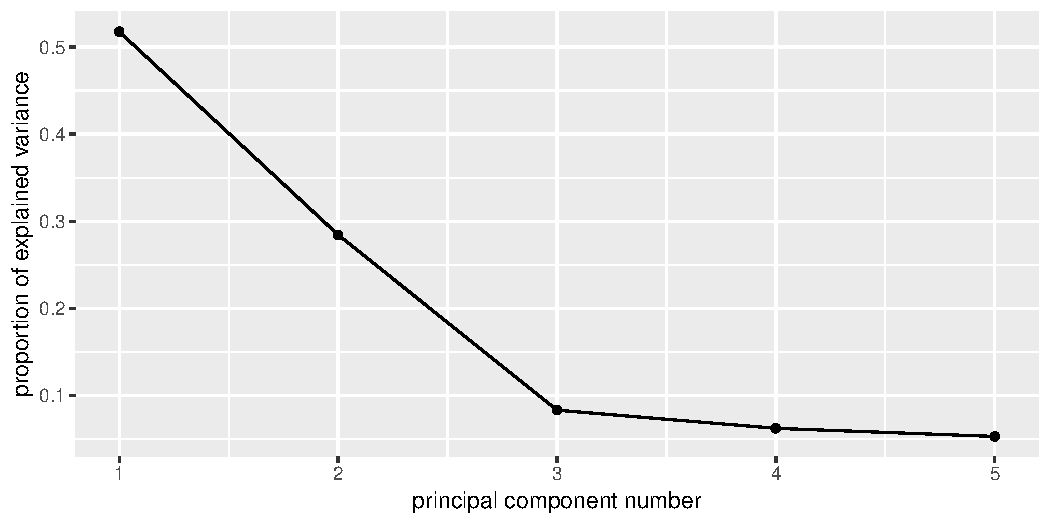
\includegraphics[width=\maxwidth]{figure/unnamed-chunk-27-1} 

\end{knitrout}
  
  
\end{frame}

\begin{frame}[fragile]{Comments on try 1}

  \begin{itemize}
\item Best: $\lambda$ just less than zero.
\item Hard to see scale. 
\item Focus on $\lambda$ in $(-0.3,0.1)$:
{\small    
 
\begin{knitrout}
\definecolor{shadecolor}{rgb}{0.969, 0.969, 0.969}\color{fgcolor}\begin{kframe}
\begin{alltt}
\hlstd{my.lambda}\hlkwb{=}\hlkwd{seq}\hlstd{(}\hlopt{-}\hlnum{0.3}\hlstd{,}\hlnum{0.1}\hlstd{,}\hlnum{0.01}\hlstd{)}
\hlstd{my.lambda}
\end{alltt}
\begin{verbatim}
 [1] -0.30 -0.29 -0.28 -0.27 -0.26 -0.25 -0.24 -0.23 -0.22
[10] -0.21 -0.20 -0.19 -0.18 -0.17 -0.16 -0.15 -0.14 -0.13
[19] -0.12 -0.11 -0.10 -0.09 -0.08 -0.07 -0.06 -0.05 -0.04
[28] -0.03 -0.02 -0.01  0.00  0.01  0.02  0.03  0.04  0.05
[37]  0.06  0.07  0.08  0.09  0.10
\end{verbatim}
\end{kframe}
\end{knitrout}
}


\end{itemize}

  
  
\end{frame}




\begin{frame}[fragile]{Try 2}

 
\begin{knitrout}
\definecolor{shadecolor}{rgb}{0.969, 0.969, 0.969}\color{fgcolor}\begin{kframe}
\begin{alltt}
\hlkwd{boxcox}\hlstd{(tp}\hlopt{~}\hlstd{phyheal}\hlopt{+}\hlstd{menheal}\hlopt{+}\hlstd{stress,}\hlkwc{lambda}\hlstd{=my.lambda)}
\end{alltt}
\end{kframe}
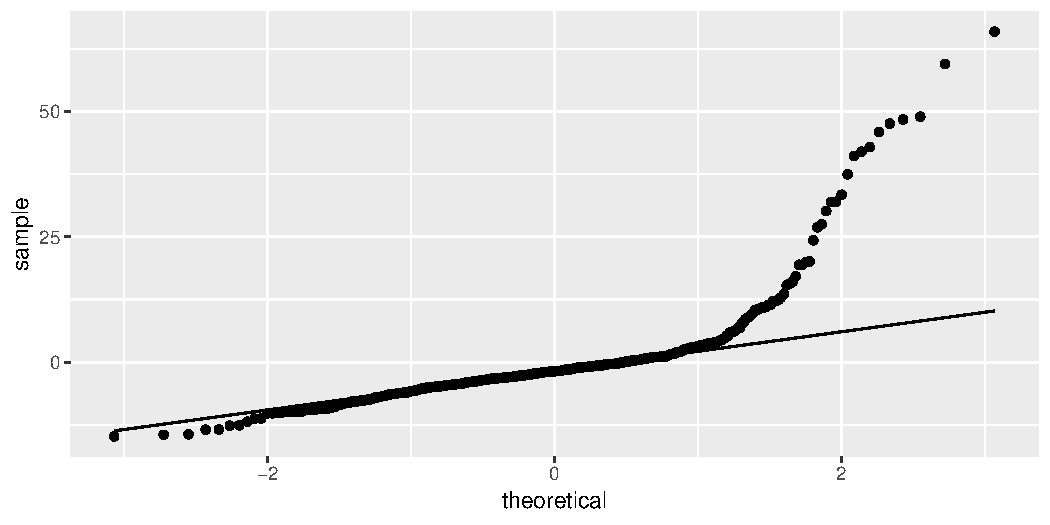
\includegraphics[width=\maxwidth]{figure/unnamed-chunk-29-1} 

\end{knitrout}

  

\end{frame}

\begin{frame}[fragile]{Comments}
  
\begin{itemize}
\item Best: $\lambda$ just about $-0.07$.
\item CI for $\lambda$ about $(-0.14,0.01)$.
\item Only nearby round number: $\lambda=0$, log transformation.
\item So we made lucky guess with log before!
\end{itemize}
  
  
\end{frame}


\begin{frame}[fragile]{Testing more than one $x$ at once}

The $t$-tests test only whether one variable could be taken out of the
regression you're looking at. To test significance of more than one
variable at once, fit model with and without variables and use
\texttt{anova} to compare fit of models:


{\small
\begin{knitrout}
\definecolor{shadecolor}{rgb}{0.969, 0.969, 0.969}\color{fgcolor}\begin{kframe}
\begin{alltt}
\hlstd{visits.5}\hlkwb{=}\hlkwd{lm}\hlstd{(lgtime}\hlopt{~}\hlstd{phyheal}\hlopt{+}\hlstd{menheal}\hlopt{+}\hlstd{stress)}
\hlstd{visits.6}\hlkwb{=}\hlkwd{lm}\hlstd{(lgtime}\hlopt{~}\hlstd{stress)}
\hlkwd{anova}\hlstd{(visits.6,visits.5)}
\end{alltt}
\begin{verbatim}
Analysis of Variance Table

Model 1: lgtime ~ stress
Model 2: lgtime ~ phyheal + menheal + stress
  Res.Df    RSS Df Sum of Sq      F    Pr(>F)    
1    463 371.47                                  
2    461 268.01  2    103.46 88.984 < 2.2e-16 ***
---
Signif. codes:  
0 '***' 0.001 '**' 0.01 '*' 0.05 '.' 0.1 ' ' 1
\end{verbatim}
\end{kframe}
\end{knitrout}
}


\end{frame}

\begin{frame}[fragile]{Results of tests}


\begin{itemize}

\item Models don't fit equally well, so big one fits better.
\item Or ``taking both variables out makes the fit worse, so don't do it''.
\item   Taking out those $x$'s
  is a mistake. Or putting them in is a good idea.
\end{itemize}
  
\end{frame}

\begin{frame}[fragile]{The punting data}

  Data set \verb-punting.dat- contains 4 variables for 13 right-footed
  football kickers (punters): left leg and right leg strength (lbs),
  distance punted (ft), another variable called ``fred''. Predict
  punting distance from other variables:

 
\begin{knitrout}
\definecolor{shadecolor}{rgb}{0.969, 0.969, 0.969}\color{fgcolor}\begin{kframe}
\begin{alltt}
\hlstd{punting}\hlkwb{=}\hlkwd{read.table}\hlstd{(}\hlstr{"punting.txt"}\hlstd{,}\hlkwc{header}\hlstd{=T)}
\hlkwd{head}\hlstd{(punting)}
\end{alltt}
\begin{verbatim}
  left right   punt fred
1  170   170 162.50  171
2  130   140 144.00  136
3  170   180 174.50  174
4  160   160 163.50  161
5  150   170 192.00  159
6  150   150 171.75  151
\end{verbatim}
\begin{alltt}
\hlkwd{attach}\hlstd{(punting)}
\hlstd{punting.1}\hlkwb{=}\hlkwd{lm}\hlstd{(punt}\hlopt{~}\hlstd{left}\hlopt{+}\hlstd{right}\hlopt{+}\hlstd{fred)}
\end{alltt}
\end{kframe}
\end{knitrout}
  
  
\end{frame}

\begin{frame}[fragile]{Regression output}

{\small
 
\begin{knitrout}
\definecolor{shadecolor}{rgb}{0.969, 0.969, 0.969}\color{fgcolor}\begin{kframe}
\begin{alltt}
\hlkwd{summary}\hlstd{(punting.1)}
\end{alltt}
\begin{verbatim}

Call:
lm(formula = punt ~ left + right + fred)

Residuals:
     Min       1Q   Median       3Q      Max 
-14.9325 -11.5618  -0.0315   9.0415  20.0886 

Coefficients:
            Estimate Std. Error t value Pr(>|t|)
(Intercept)  -4.6855    29.1172  -0.161    0.876
left          0.2679     2.1111   0.127    0.902
right         1.0524     2.1477   0.490    0.636
fred         -0.2672     4.2266  -0.063    0.951

Residual standard error: 14.68 on 9 degrees of freedom
Multiple R-squared:  0.7781,	Adjusted R-squared:  0.7042 
F-statistic: 10.52 on 3 and 9 DF,  p-value: 0.00267
\end{verbatim}
\end{kframe}
\end{knitrout}
}


\end{frame}


\begin{frame}{Comments}

  \begin{itemize}
  \item Overall regression strongly significant, R-sq high.
  \item None of the $x$'s significant! Why?
  \item $t$-tests only say that you could take any one of the $x$'s out without damaging the fit; doesn't matter which one.
  \item Explanation: look at {\em correlations}. 
  \end{itemize}
\end{frame}

\begin{frame}[fragile]{The correlations}  

 
\begin{knitrout}
\definecolor{shadecolor}{rgb}{0.969, 0.969, 0.969}\color{fgcolor}\begin{kframe}
\begin{alltt}
\hlkwd{cor}\hlstd{(punting)}
\end{alltt}
\begin{verbatim}
           left     right      punt      fred
left  1.0000000 0.8957224 0.8117368 0.9722632
right 0.8957224 1.0000000 0.8805469 0.9728784
punt  0.8117368 0.8805469 1.0000000 0.8679507
fred  0.9722632 0.9728784 0.8679507 1.0000000
\end{verbatim}
\end{kframe}
\end{knitrout}
  

\begin{itemize}
\item {\em All} correlations are high: $x$'s with \verb-punt- (good) and
with each other (bad, at least confusing).
\item What to do? Probably do just as well to pick one variable, say
\texttt{right} since kickers are right-footed.
\end{itemize}



\end{frame}

\begin{frame}[fragile]{Just \texttt{right}}

  {\small
 
\begin{knitrout}
\definecolor{shadecolor}{rgb}{0.969, 0.969, 0.969}\color{fgcolor}\begin{kframe}
\begin{alltt}
\hlstd{punting.2}\hlkwb{=}\hlkwd{lm}\hlstd{(punt}\hlopt{~}\hlstd{right)}
\hlkwd{anova}\hlstd{(punting.2,punting.1)}
\end{alltt}
\begin{verbatim}
Analysis of Variance Table

Model 1: punt ~ right
Model 2: punt ~ left + right + fred
  Res.Df    RSS Df Sum of Sq      F Pr(>F)
1     11 1962.5                           
2      9 1938.2  2    24.263 0.0563 0.9456
\end{verbatim}
\end{kframe}
\end{knitrout}
}
  

No significant loss by dropping other two variables.

\end{frame}

\begin{frame}[fragile]{Comparing R-squareds}


{\small
\begin{knitrout}
\definecolor{shadecolor}{rgb}{0.969, 0.969, 0.969}\color{fgcolor}\begin{kframe}
\begin{alltt}
\hlkwd{summary}\hlstd{(punting.1)}\hlopt{$}\hlstd{r.squared}
\end{alltt}
\begin{verbatim}
[1] 0.7781401
\end{verbatim}
\begin{alltt}
\hlkwd{summary}\hlstd{(punting.2)}\hlopt{$}\hlstd{r.squared}
\end{alltt}
\begin{verbatim}
[1] 0.7753629
\end{verbatim}
\end{kframe}
\end{knitrout}
}

Basically no difference. In regression (over), \texttt{right} significant:
  

  
\end{frame}

\begin{frame}[fragile]{Regression results}

{\footnotesize
 
\begin{knitrout}
\definecolor{shadecolor}{rgb}{0.969, 0.969, 0.969}\color{fgcolor}\begin{kframe}
\begin{alltt}
\hlkwd{summary}\hlstd{(punting.2)}
\end{alltt}
\begin{verbatim}

Call:
lm(formula = punt ~ right)

Residuals:
     Min       1Q   Median       3Q      Max 
-15.7576 -11.0611   0.3656   7.8890  19.0423 

Coefficients:
            Estimate Std. Error t value Pr(>|t|)    
(Intercept)  -3.6930    25.2649  -0.146    0.886    
right         1.0427     0.1692   6.162 7.09e-05 ***
---
Signif. codes:  
0 '***' 0.001 '**' 0.01 '*' 0.05 '.' 0.1 ' ' 1

Residual standard error: 13.36 on 11 degrees of freedom
Multiple R-squared:  0.7754,	Adjusted R-squared:  0.7549 
F-statistic: 37.97 on 1 and 11 DF,  p-value: 7.088e-05
\end{verbatim}
\end{kframe}
\end{knitrout}
}
 
\end{frame}


\begin{frame}[fragile]{But\ldots}
  
  \begin{itemize}
  \item Maybe we got the \emph{form} of the relationship with
    \texttt{left} wrong.
  \item Check: plot \emph{residuals} from previous regression (without
    \texttt{left}) against \texttt{left}.
  \item Residuals here are ``punting distance adjusted for right
    leg strength''.
  \item If there is some kind of relationship with \texttt{left}, we
    should include in model.
  \end{itemize}
  
\end{frame}

\begin{frame}[fragile]{Residuals against \texttt{left}}
  
\begin{knitrout}
\definecolor{shadecolor}{rgb}{0.969, 0.969, 0.969}\color{fgcolor}\begin{kframe}
\begin{alltt}
\hlstd{r}\hlkwb{=}\hlkwd{resid}\hlstd{(punting.2)}
\hlkwd{ggplot}\hlstd{(punting,}\hlkwd{aes}\hlstd{(}\hlkwc{x}\hlstd{=left,}\hlkwc{y}\hlstd{=r))}\hlopt{+}\hlkwd{geom_point}\hlstd{()}\hlopt{+}\hlkwd{geom_smooth}\hlstd{()}
\end{alltt}


{\ttfamily\noindent\itshape\color{messagecolor}{`geom\_smooth()` using method = 'loess'}}\end{kframe}
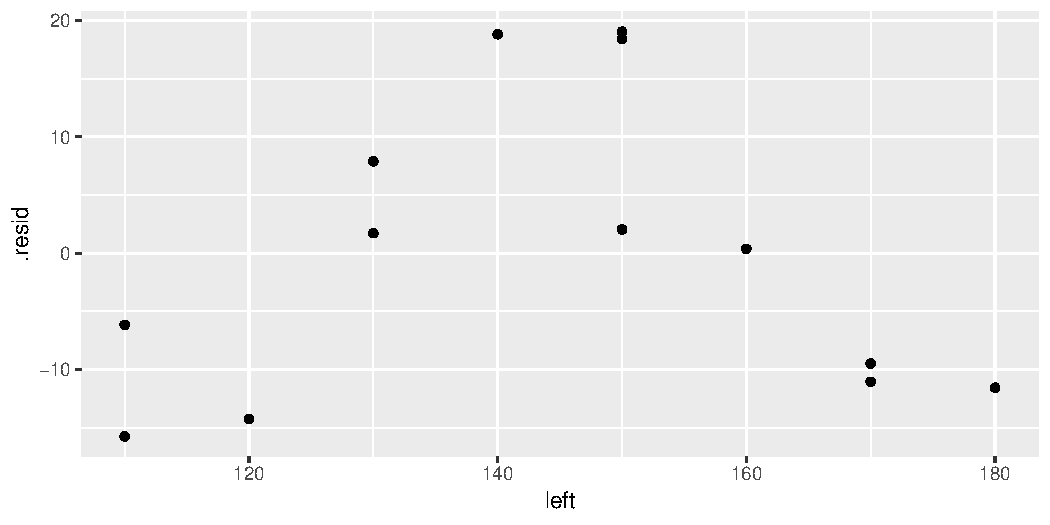
\includegraphics[width=\maxwidth]{figure/basingstoke-1} 

\end{knitrout}
  
\end{frame}

\begin{frame}[fragile]{Comments}
  
  \begin{itemize}
  \item There is a \emph{curved} relationship with \texttt{left}.
  \item We should add \texttt{left}-squared to the regression (and
    therefore put \texttt{left} back in when we do that):
    
\begin{knitrout}
\definecolor{shadecolor}{rgb}{0.969, 0.969, 0.969}\color{fgcolor}\begin{kframe}
\begin{alltt}
\hlstd{leftsq}\hlkwb{=}\hlstd{left}\hlopt{*}\hlstd{left}
\hlstd{punting.3}\hlkwb{=}\hlkwd{lm}\hlstd{(punt}\hlopt{~}\hlstd{left}\hlopt{+}\hlstd{leftsq}\hlopt{+}\hlstd{right)}
\end{alltt}
\end{kframe}
\end{knitrout}
  \end{itemize}
  
\end{frame}

\begin{frame}[fragile]{Regression with \texttt{left}-squared}
  
  {\footnotesize
\begin{knitrout}
\definecolor{shadecolor}{rgb}{0.969, 0.969, 0.969}\color{fgcolor}\begin{kframe}
\begin{alltt}
\hlkwd{summary}\hlstd{(punting.3)}
\end{alltt}
\begin{verbatim}

Call:
lm(formula = punt ~ left + leftsq + right)

Residuals:
     Min       1Q   Median       3Q      Max 
-11.3777  -5.3599   0.0459   4.5088  13.2669 

Coefficients:
              Estimate Std. Error t value Pr(>|t|)   
(Intercept) -4.623e+02  9.902e+01  -4.669  0.00117 **
left         6.888e+00  1.462e+00   4.710  0.00110 **
leftsq      -2.302e-02  4.927e-03  -4.672  0.00117 **
right        7.396e-01  2.292e-01   3.227  0.01038 * 
---
Signif. codes:  
0 '***' 0.001 '**' 0.01 '*' 0.05 '.' 0.1 ' ' 1

Residual standard error: 7.931 on 9 degrees of freedom
Multiple R-squared:  0.9352,	Adjusted R-squared:  0.9136 
F-statistic:  43.3 on 3 and 9 DF,  p-value: 1.13e-05
\end{verbatim}
\end{kframe}
\end{knitrout}
}

  
\end{frame}

\begin{frame}[fragile]{Comments}
  
\begin{itemize}
\item This was definitely a good idea (R-squared has clearly increased).
\item We would never have seen it without plotting residuals from
  \texttt{punting.2} (without \texttt{left}) against \texttt{left}.
\item Negative slope for \texttt{leftsq} means that increased left-leg
  strength only increases punting distance up to a point: beyond that,
  it decreases again.
\end{itemize}
  
  
\end{frame}

\section{Logistic regression (ordinal/nominal response)}
\frame{\sectionpage}


\begin{frame}{Logistic regression}

  \begin{itemize}
  \item When response variable is measured/counted, regression can work well.
  \item But what if response is yes/no, lived/died, success/failure?
  \item Model {\em probability} of success.
  \item Probability must be between 0 and 1; need method that ensures this.
  \item {\em Logistic regression} does this. In R, is a
    \emph{generalized linear model} with binomial ``family'': 
\texttt{glm(y\textasciitilde x,family="binomial")}
    
  \item Begin with simplest case.
    
  \end{itemize}
  
\end{frame}

\begin{frame}[fragile]{The rats, part 1}

  \begin{itemize}
  \item Rats given dose of some poison; either live or die:

{\scriptsize
\begin{verbatim}
dose status
0 lived
1 died
2 lived
3 lived
4 died
5 died
\end{verbatim}
}
\item Basic logistic regression analysis:

{\footnotesize
 
\begin{knitrout}
\definecolor{shadecolor}{rgb}{0.969, 0.969, 0.969}\color{fgcolor}\begin{kframe}
\begin{alltt}
\hlstd{rats}\hlkwb{=}\hlkwd{read.table}\hlstd{(}\hlstr{"rat.txt"}\hlstd{,}\hlkwc{header}\hlstd{=T)}
\hlstd{rats}
\end{alltt}
\begin{verbatim}
##   dose status
## 1    0  lived
## 2    1   died
## 3    2  lived
## 4    3  lived
## 5    4   died
## 6    5   died
\end{verbatim}
\begin{alltt}
\hlkwd{attach}\hlstd{(rats)}
\hlstd{rats.1}\hlkwb{=}\hlkwd{glm}\hlstd{(status}\hlopt{~}\hlstd{dose,}\hlkwc{family}\hlstd{=}\hlstr{"binomial"}\hlstd{)}
\end{alltt}
\end{kframe}
\end{knitrout}
}
  

  \end{itemize}
  



\end{frame}
  

\begin{frame}[fragile]{Output}

  {\footnotesize
 
\begin{knitrout}
\definecolor{shadecolor}{rgb}{0.969, 0.969, 0.969}\color{fgcolor}\begin{kframe}
\begin{alltt}
\hlkwd{summary}\hlstd{(rats.1)}
\end{alltt}
\begin{verbatim}
## 
## Call:
## glm(formula = status ~ dose, family = "binomial")
## 
## Deviance Residuals: 
##       1        2        3        4        5        6  
##  0.5835  -1.6254   1.0381   1.3234  -0.7880  -0.5835  
## 
## Coefficients:
##             Estimate Std. Error z value Pr(>|z|)
## (Intercept)   1.6841     1.7979   0.937    0.349
## dose         -0.6736     0.6140  -1.097    0.273
## 
## (Dispersion parameter for binomial family taken to be 1)
## 
##     Null deviance: 8.3178  on 5  degrees of freedom
## Residual deviance: 6.7728  on 4  degrees of freedom
## AIC: 10.773
## 
## Number of Fisher Scoring iterations: 4
\end{verbatim}
\end{kframe}
\end{knitrout}
}   

\end{frame}


\begin{frame}{Interpreting the output}
  \begin{itemize}
  \item Like (multiple) regression, get
   tests of significance of individual $x$'s
  \item     Here not significant (only 6 observations).
  \item ``Slope'' for dose is negative, meaning that as dose increases, probability of event modelled (survival) decreases.

\end{itemize}

\end{frame}

\begin{frame}[fragile]{Output part 2: predicted survival probs}

  
 
\begin{knitrout}
\definecolor{shadecolor}{rgb}{0.969, 0.969, 0.969}\color{fgcolor}\begin{kframe}
\begin{alltt}
\hlstd{p}\hlkwb{=}\hlkwd{predict}\hlstd{(rats.1,}\hlkwc{type}\hlstd{=}\hlstr{"response"}\hlstd{)}
\hlkwd{cbind}\hlstd{(rats,p)}
\end{alltt}
\begin{verbatim}
##   dose status         p
## 1    0  lived 0.8434490
## 2    1   died 0.7331122
## 3    2  lived 0.5834187
## 4    3  lived 0.4165813
## 5    4   died 0.2668878
## 6    5   died 0.1565510
\end{verbatim}
\end{kframe}
\end{knitrout}
  
\end{frame}




\begin{frame}[fragile]{The rats, more}

  \begin{itemize}
  \item More realistic: more rats at each dose (say 10).
  \item Listing each rat on one line makes a big data file.
  \item Use format below: dose, number of survivals, number of deaths.
\begin{verbatim}
dose lived died
   0    10    0
   1     7    3 
   2     6    4 
   3     4    6 
   4     2    8 
   5     1    9  
\end{verbatim}


  \item 6 lines of data correspond to 60 actual rats.

  \item Saved in \texttt{rat2.txt}.

  \end{itemize}
  
\end{frame}

\begin{frame}[fragile]{Code for this logistic regression}

 
\begin{knitrout}
\definecolor{shadecolor}{rgb}{0.969, 0.969, 0.969}\color{fgcolor}\begin{kframe}
\begin{alltt}
\hlkwd{detach}\hlstd{(rats)}
\hlstd{rat2}\hlkwb{=}\hlkwd{read.table}\hlstd{(}\hlstr{"rat2.txt"}\hlstd{,}\hlkwc{header}\hlstd{=T)}
\hlstd{rat2}
\end{alltt}
\begin{verbatim}
##   dose lived died
## 1    0    10    0
## 2    1     7    3
## 3    2     6    4
## 4    3     4    6
## 5    4     2    8
## 6    5     1    9
\end{verbatim}
\begin{alltt}
\hlkwd{attach}\hlstd{(rat2)}
\hlstd{response}\hlkwb{=}\hlkwd{cbind}\hlstd{(lived,died)}
\hlstd{rat2.1}\hlkwb{=}\hlkwd{glm}\hlstd{(response}\hlopt{~}\hlstd{dose,}\hlkwc{family}\hlstd{=}\hlstr{"binomial"}\hlstd{)}
\end{alltt}
\end{kframe}
\end{knitrout}
  
\begin{itemize}
\item Note construction of \emph{two-column} response, \#survivals in
  first column, \#deaths in second.
\end{itemize}


  
\end{frame}

\begin{frame}[fragile]{Output}

{\footnotesize  
 
\begin{knitrout}
\definecolor{shadecolor}{rgb}{0.969, 0.969, 0.969}\color{fgcolor}\begin{kframe}
\begin{alltt}
\hlkwd{summary}\hlstd{(rat2.1)}
\end{alltt}
\begin{verbatim}
## 
## Call:
## glm(formula = response ~ dose, family = "binomial")
## 
## Deviance Residuals: 
##       1        2        3        4        5        6  
##  1.3421  -0.7916  -0.1034   0.1034   0.0389   0.1529  
## 
## Coefficients:
##             Estimate Std. Error z value Pr(>|z|)    
## (Intercept)   2.3619     0.6719   3.515 0.000439 ***
## dose         -0.9448     0.2351  -4.018 5.87e-05 ***
## ---
## Signif. codes:  0 '***' 0.001 '**' 0.01 '*' 0.05 '.' 0.1 ' ' 1
## 
## (Dispersion parameter for binomial family taken to be 1)
## 
##     Null deviance: 27.530  on 5  degrees of freedom
## Residual deviance:  2.474  on 4  degrees of freedom
## AIC: 18.94
## 
## Number of Fisher Scoring iterations: 4
\end{verbatim}
\end{kframe}
\end{knitrout}
}
  

\end{frame}

\begin{frame}[fragile]{Predicted survival probs}

 
\begin{knitrout}
\definecolor{shadecolor}{rgb}{0.969, 0.969, 0.969}\color{fgcolor}\begin{kframe}
\begin{alltt}
\hlstd{p}\hlkwb{=}\hlkwd{predict}\hlstd{(rat2.1,}\hlkwc{type}\hlstd{=}\hlstr{"response"}\hlstd{)}
\hlkwd{cbind}\hlstd{(rat2,p)}
\end{alltt}
\begin{verbatim}
##   dose lived died         p
## 1    0    10    0 0.9138762
## 2    1     7    3 0.8048905
## 3    2     6    4 0.6159474
## 4    3     4    6 0.3840526
## 5    4     2    8 0.1951095
## 6    5     1    9 0.0861238
\end{verbatim}
\end{kframe}
\end{knitrout}
  
  

  
\end{frame}

\begin{frame}[fragile]{Comments}

\begin{itemize}
\item Significant effect of dose. 
\item Effect of larger dose is to decrease survival probability
  (``slope'' negative; also see in decreasing predictions.)
\end{itemize}
  
\end{frame}


\begin{frame}{Multiple logistic regression}

  \begin{itemize}
  \item With more than one $x$, works much like multiple regression.
  \item Example: study of patients with blood poisoning severe enough to warrant surgery. Relate survival to other potential risk factors.
  \item Variables, 1=present, 0=absent:
    \begin{itemize}
    \item survival (death from sepsis=1), response
    \item shock
    \item malnutrition
    \item alcoholism
    \item age (as numerical variable)
    \item bowel infarction
    \end{itemize}
  \item See what relates to death.
  \end{itemize}


  
\end{frame}

\begin{frame}[fragile]{Read in data and fit model}

 
\begin{knitrout}
\definecolor{shadecolor}{rgb}{0.969, 0.969, 0.969}\color{fgcolor}\begin{kframe}
\begin{alltt}
\hlkwd{detach}\hlstd{(rat2)}
\hlstd{sepsis}\hlkwb{=}\hlkwd{read.table}\hlstd{(}\hlstr{"sepsis.txt"}\hlstd{,}\hlkwc{header}\hlstd{=T)}
\hlkwd{head}\hlstd{(sepsis)}
\end{alltt}
\begin{verbatim}
##   death shock malnut alcohol age bowelinf
## 1     0     0      0       0  56        0
## 2     0     0      0       0  80        0
## 3     0     0      0       0  61        0
## 4     0     0      0       0  26        0
## 5     0     0      0       0  53        0
## 6     1     0      1       0  87        0
\end{verbatim}
\begin{alltt}
\hlkwd{attach}\hlstd{(sepsis)}
\hlstd{sepsis.1}\hlkwb{=}\hlkwd{glm}\hlstd{(death}\hlopt{~}\hlstd{shock}\hlopt{+}\hlstd{malnut}\hlopt{+}\hlstd{alcohol}\hlopt{+}\hlstd{age}\hlopt{+}
              \hlstd{bowelinf,}\hlkwc{family}\hlstd{=}\hlstr{"binomial"}\hlstd{)}
\end{alltt}
\end{kframe}
\end{knitrout}
  

\end{frame}

\begin{frame}[fragile]{Output part 1}

 
\begin{knitrout}
\definecolor{shadecolor}{rgb}{0.969, 0.969, 0.969}\color{fgcolor}\begin{kframe}
\begin{alltt}
\hlkwd{summary}\hlstd{(sepsis.1)}\hlopt{$}\hlstd{coefficients}
\end{alltt}
\begin{verbatim}
##                Estimate Std. Error   z value     Pr(>|z|)
## (Intercept) -9.75390560 2.54169523 -3.837559 0.0001242633
## shock        3.67386585 1.16481138  3.154044 0.0016102504
## malnut       1.21658106 0.72822359  1.670615 0.0947978002
## alcohol      3.35488462 0.98210260  3.416023 0.0006354299
## age          0.09215268 0.03032368  3.038968 0.0023739015
## bowelinf     2.79758637 1.16397170  2.403483 0.0162397151
\end{verbatim}
\end{kframe}
\end{knitrout}
%$

\begin{itemize}
\item All P-values fairly small
\item but \texttt{malnut} not significant: remove.
\end{itemize}


\end{frame}

\begin{frame}[fragile]{Removing \texttt{malnut}}

 
\begin{knitrout}
\definecolor{shadecolor}{rgb}{0.969, 0.969, 0.969}\color{fgcolor}\begin{kframe}
\begin{alltt}
\hlstd{sepsis.2}\hlkwb{=}\hlkwd{glm}\hlstd{(death}\hlopt{~}\hlstd{shock}\hlopt{+}\hlstd{alcohol}\hlopt{+}\hlstd{age}\hlopt{+}
              \hlstd{bowelinf,}\hlkwc{family}\hlstd{=}\hlstr{"binomial"}\hlstd{)}
\hlkwd{summary}\hlstd{(sepsis.2)}\hlopt{$}\hlstd{coefficients}
\end{alltt}
\begin{verbatim}
##                Estimate Std. Error   z value     Pr(>|z|)
## (Intercept) -8.89458992 2.31689479 -3.839013 0.0001235297
## shock        3.70119321 1.10353465  3.353944 0.0007966854
## alcohol      3.18590397 0.91724569  3.473338 0.0005140283
## age          0.08983175 0.02921528  3.074821 0.0021062897
## bowelinf     2.38646847 1.07226618  2.225631 0.0260389310
\end{verbatim}
\end{kframe}
\end{knitrout}

\begin{itemize}
\item Everything significant now.
\end{itemize}
  
 
  
\end{frame}

\begin{frame}[fragile]{Comments}

%$  
  \begin{itemize}
\item Most of the original $x$'s helped predict death. Only \texttt{malnut} seemed not to add anything.
\item Removed \texttt{malnut} and tried again.
\item Everything remaining is significant (though \texttt{bowelinf}
  actually became \emph{less} significant).
\item All coefficients are \emph{positive}, so having any of the risk
  factors (or being older)
  \emph{increases} risk of death.  
\end{itemize}

\end{frame}

\begin{frame}[fragile]{Predictions from model without ``malnut''}
  
  \begin{itemize}
  \item A few chosen at random. Define vector containing rows you
    want, then pick out of data frame and predictions:

    {\small
\begin{knitrout}
\definecolor{shadecolor}{rgb}{0.969, 0.969, 0.969}\color{fgcolor}\begin{kframe}
\begin{alltt}
\hlstd{sepsis.pred}\hlkwb{=}\hlkwd{predict}\hlstd{(sepsis.2,}\hlkwc{type}\hlstd{=}\hlstr{"response"}\hlstd{)}
\hlstd{myrows}\hlkwb{=}\hlkwd{c}\hlstd{(}\hlnum{4}\hlstd{,}\hlnum{1}\hlstd{,}\hlnum{2}\hlstd{,}\hlnum{11}\hlstd{,}\hlnum{32}\hlstd{)}
\hlkwd{cbind}\hlstd{(sepsis[myrows,],}\hlkwc{p}\hlstd{=sepsis.pred[myrows])}
\end{alltt}
\begin{verbatim}
##    death shock malnut alcohol age bowelinf           p
## 4      0     0      0       0  26        0 0.001415347
## 1      0     0      0       0  56        0 0.020552383
## 2      0     0      0       0  80        0 0.153416834
## 11     1     0      0       1  66        1 0.931290137
## 32     1     0      0       1  49        0 0.213000997
\end{verbatim}
\end{kframe}
\end{knitrout}
}

\item Survival chances pretty good if no risk factors, though decreasing with age.
\item Having more than one risk factor reduces survival chances dramatically.
\item Usually model does a good job of predicting survival, but occasionally someone dies who was predicted to survive.
  \end{itemize}
  
\end{frame}

\begin{frame}[fragile]{Assessing proportionality of odds for age}
  \begin{itemize}
  \item An assumption we made is that log-odds of survival depends
    linearly on age.
  \item Hard to get your head around, but 
    basic idea is that survival chances go continuously up (or down)
    with age, instead of (for example) going up and then down.
  \item In this case, seems reasonable, but should check:

\begin{knitrout}
\definecolor{shadecolor}{rgb}{0.969, 0.969, 0.969}\color{fgcolor}\begin{kframe}
\begin{alltt}
\hlkwd{library}\hlstd{(tidyverse)}
\end{alltt}


{\ttfamily\noindent\itshape\color{messagecolor}{\#\# Loading tidyverse: ggplot2\\\#\# Loading tidyverse: tibble\\\#\# Loading tidyverse: tidyr\\\#\# Loading tidyverse: readr\\\#\# Loading tidyverse: purrr\\\#\# Loading tidyverse: dplyr}}

{\ttfamily\noindent\itshape\color{messagecolor}{\#\# Conflicts with tidy packages ----------------------------------------------}}

{\ttfamily\noindent\itshape\color{messagecolor}{\#\# filter(): dplyr, stats\\\#\# lag():\ \ \ \ dplyr, stats}}\end{kframe}
\end{knitrout}
  \end{itemize}
    

\end{frame}
 

\begin{frame}[fragile]{Residuals vs.\ age}

 
\begin{knitrout}
\definecolor{shadecolor}{rgb}{0.969, 0.969, 0.969}\color{fgcolor}\begin{kframe}
\begin{alltt}
\hlstd{r}\hlkwb{=}\hlkwd{residuals}\hlstd{(sepsis.2)}
\hlkwd{ggplot}\hlstd{(sepsis,}\hlkwd{aes}\hlstd{(}\hlkwc{x}\hlstd{=age,}\hlkwc{y}\hlstd{=r))}\hlopt{+}\hlkwd{geom_point}\hlstd{()}
\end{alltt}
\end{kframe}
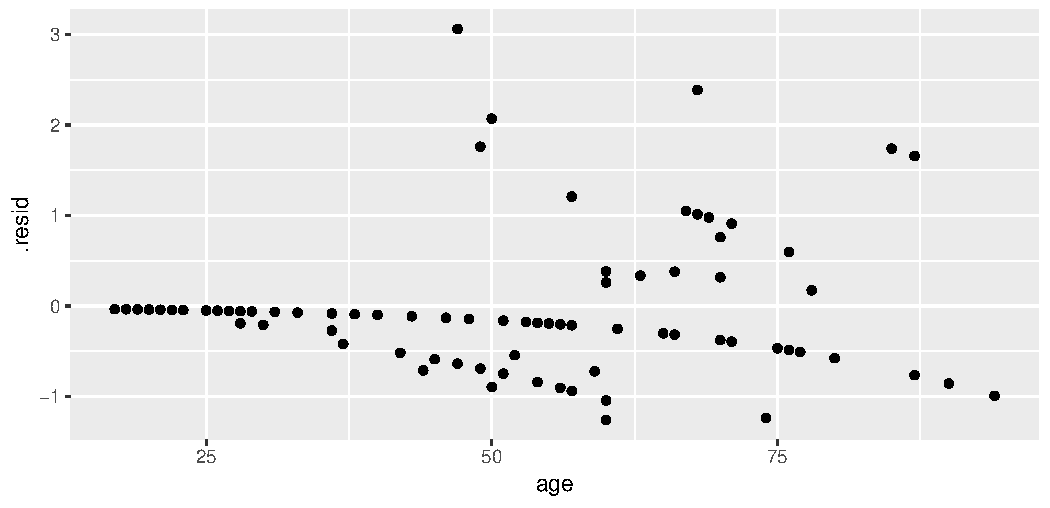
\includegraphics[width=\maxwidth]{figure/virtusentella-1} 

\end{knitrout}
  
  
\begin{itemize}
\item No apparent problems overall.
\item Confusing ``line'' across: no risk factors, survived. 
\end{itemize}
  
\end{frame}

\begin{frame}[fragile]{Probability and odds}
  
  \begin{itemize}
  \item For probability $p$, odds is $p/(1-p)$. Examples:
    \vfill
    \begin{tabular}{rrrl}
      \hline
      Prob.\ & Odds & log-odds & in words\\
      \hline
      0.5 & $0.5/0.5=1/1=1.00$ & 0.00 &  ``even money''\\
      0.1 & $0.1/0.9=1/9=0.11$ & $-2.20$ & ``9 to 1''\\
      0.4 & $0.4/0.6=1/1.5=0.67$ & $-0.41$ & ``1.5 to 1''\\
      0.8 & $0.8/0.2=4/1=4.00$ & 1.39 & ``4 to 1 on''\\
      \hline
    \end{tabular}
    \vfill
  \item Gamblers use odds: if you win at 9 to 1 odds, get original
    stake back plus 9 times the stake.
  \item Probability has to be between 0 and 1
  \item Odds between 0 and infinity
  \item \emph{Log}-odds can be anything: any log-odds corresponds to
    valid probability.
  \end{itemize}
  
\end{frame}

\begin{frame}[fragile]{Odds ratio}
  
  \begin{itemize}
  \item Suppose 90 of 100 men drank wine last week, but only 20 of 100 women.
  \item Prob of man drinking wine $90/100=0.9$, woman $20/100=0.2$.
  \item Odds of man drinking wine $0.9/0.1=9$, woman $0.2/0.8=0.25$.
  \item Ratio of odds is $9/0.25=36$.
  \item Way of quantifying difference between men and women: ``odds of
    drinking wine 36 times larger for males than females''. 
  \end{itemize}
  
\end{frame}

\begin{frame}[fragile]{Multiplying the odds}

  \begin{itemize}
  \item Can interpret slopes by taking ``exp'' of them. I ignore intercept.

 
\begin{knitrout}
\definecolor{shadecolor}{rgb}{0.969, 0.969, 0.969}\color{fgcolor}\begin{kframe}
\begin{alltt}
\hlstd{cc}\hlkwb{=}\hlkwd{exp}\hlstd{(}\hlkwd{coef}\hlstd{(sepsis.2)[}\hlopt{-}\hlnum{1}\hlstd{])}
\hlkwd{round}\hlstd{(cc,}\hlnum{2}\hlstd{)}
\end{alltt}
\begin{verbatim}
##    shock  alcohol      age bowelinf 
##    40.50    24.19     1.09    10.88
\end{verbatim}
\end{kframe}
\end{knitrout}

\item These say ``how much do you \emph{multiply} odds of death by
    for increase of 1 in corresponding risk factor?'' Or, what is odds
    ratio for that factor being 1 (present) vs.\ 0 (absent)?
  \item Eg.\ being alcoholic vs.\ not increases odds of death by 24 times
  \item One year older multiplies odds by about 1.1 times. Over 40 years,
    about  $1.09^{40}=31$ times. 
  \item Tidy up:
 
\begin{knitrout}
\definecolor{shadecolor}{rgb}{0.969, 0.969, 0.969}\color{fgcolor}\begin{kframe}
\begin{alltt}
\hlkwd{detach}\hlstd{(sepsis)}
\end{alltt}
\end{kframe}
\end{knitrout}
    

  \end{itemize}
  
\end{frame}

\begin{frame}[fragile]{Odds ratio and relative risk}
  
  \begin{itemize}
  \item \textbf{Relative risk} is ratio of probabilities.
  \item Above: 90 of 100 men (0.9) drank wine, 20 of 100 women (0.2).
  \item Relative risk 0.9/0.2=4.5. (odds ratio was 36).
  \item When probabilities small, relative risk and odds ratio similar.
  \item Eg.\ prob of man having disease 0.02, woman 0.01.
  \item Relative risk $0.02/0.01=2$.
  \item Odds for men and for women:
 
\begin{knitrout}
\definecolor{shadecolor}{rgb}{0.969, 0.969, 0.969}\color{fgcolor}\begin{kframe}
\begin{alltt}
\hlstd{(od1}\hlkwb{=}\hlnum{0.02}\hlopt{/}\hlnum{0.98}\hlstd{)}
\end{alltt}
\begin{verbatim}
## [1] 0.02040816
\end{verbatim}
\begin{alltt}
\hlstd{(od2}\hlkwb{=}\hlnum{0.01}\hlopt{/}\hlnum{0.99}\hlstd{)}
\end{alltt}
\begin{verbatim}
## [1] 0.01010101
\end{verbatim}
\end{kframe}
\end{knitrout}

\item Odds ratio 
 
\begin{knitrout}
\definecolor{shadecolor}{rgb}{0.969, 0.969, 0.969}\color{fgcolor}\begin{kframe}
\begin{alltt}
\hlstd{od1}\hlopt{/}\hlstd{od2} \hlcom{# very close to 2}
\end{alltt}
\begin{verbatim}
## [1] 2.020408
\end{verbatim}
\end{kframe}
\end{knitrout}
  
    
  \end{itemize}
  
\end{frame}



\begin{frame}{More than 2 response categories}

  \begin{itemize}
  \item With 2 response categories, model the probability of one, and prob of other is one minus that. So doesn't matter which category you model.
  \item With more than 2 categories, have to think more carefully about the categories: are they
    \begin{itemize}
    \item {\em ordered}: you can put them in a natural order (like low, medium, high)
    \item {\em nominal}: ordering the categories doesn't make sense (like red, green, blue).
    \end{itemize}
  \item R handles both kinds of response; learn how.
  \end{itemize}
  
\end{frame}

\begin{frame}[fragile]{Ordinal response: the miners}


  \begin{itemize}
  \item 
Model probability of being in given category {\em or lower}.
\item Example: coal-miners often suffer disease pneumoconiosis. Likelihood of disease believed to be greater 
among miners who have worked longer. 
\item Severity of disease measured on categorical scale: 1 = none, 2
= moderate, 3 = severe.
\item Data are frequencies:
\begin{verbatim}
Exposure None Moderate Severe
   5.8    98      0       0
  15.0    51      2       1
  21.5    34      6       3
  27.5    35      5       8
  33.5    32      10      9
  39.5    23      7       8
  46.0    12      6      10
  51.5     4      2       5
\end{verbatim}
  
\end{itemize}
\end{frame}

\begin{frame}[fragile]{Reading the data}

 
\begin{knitrout}
\definecolor{shadecolor}{rgb}{0.969, 0.969, 0.969}\color{fgcolor}\begin{kframe}
\begin{alltt}
\hlstd{freqs}\hlkwb{=}\hlkwd{read.table}\hlstd{(}\hlstr{"miners-tab.txt"}\hlstd{,}\hlkwc{header}\hlstd{=T)}
\hlstd{freqs}
\end{alltt}
\begin{verbatim}
##   Exposure None Moderate Severe
## 1      5.8   98        0      0
## 2     15.0   51        2      1
## 3     21.5   34        6      3
## 4     27.5   35        5      8
## 5     33.5   32       10      9
## 6     39.5   23        7      8
## 7     46.0   12        6     10
## 8     51.5    4        2      5
\end{verbatim}
\end{kframe}
\end{knitrout}

  
\end{frame}

\begin{frame}[fragile]{Tidying and row proportions}
  
\begin{knitrout}
\definecolor{shadecolor}{rgb}{0.969, 0.969, 0.969}\color{fgcolor}\begin{kframe}
\begin{alltt}
\hlstd{freqs} \hlopt
  \hlkwd{gather}\hlstd{(Severity,Freq,None}\hlopt{:}\hlstd{Severe)} \hlopt
  \hlkwd{group_by}\hlstd{(Exposure)} \hlopt
  \hlkwd{mutate}\hlstd{(}\hlkwc{proportion}\hlstd{=}\hlkwd{prop.table}\hlstd{(Freq))} \hlkwb{->} \hlstd{miners}
\end{alltt}
\end{kframe}
\end{knitrout}
    

  
\end{frame}

\begin{frame}[fragile]{Result}
  
  \begin{footnotesize}
\begin{knitrout}
\definecolor{shadecolor}{rgb}{0.969, 0.969, 0.969}\color{fgcolor}\begin{kframe}
\begin{alltt}
\hlstd{miners}
\end{alltt}
\begin{verbatim}
## Source: local data frame [24 x 4]
## Groups: Exposure [8]
## 
##    Exposure Severity  Freq proportion
##       <dbl>    <chr> <int>      <dbl>
## 1       5.8     None    98 1.00000000
## 2      15.0     None    51 0.94444444
## 3      21.5     None    34 0.79069767
## 4      27.5     None    35 0.72916667
## 5      33.5     None    32 0.62745098
## 6      39.5     None    23 0.60526316
## 7      46.0     None    12 0.42857143
## 8      51.5     None     4 0.36363636
## 9       5.8 Moderate     0 0.00000000
## 10     15.0 Moderate     2 0.03703704
## # ... with 14 more rows
\end{verbatim}
\end{kframe}
\end{knitrout}
  \end{footnotesize}
  
\end{frame}

\begin{frame}[fragile]{Plot proportions against exposure}
  
\begin{knitrout}
\definecolor{shadecolor}{rgb}{0.969, 0.969, 0.969}\color{fgcolor}\begin{kframe}
\begin{alltt}
\hlkwd{ggplot}\hlstd{(miners,}\hlkwd{aes}\hlstd{(}\hlkwc{x}\hlstd{=Exposure,}\hlkwc{y}\hlstd{=proportion,}
    \hlkwc{colour}\hlstd{=Severity))}\hlopt{+}
  \hlkwd{geom_point}\hlstd{()}\hlopt{+}\hlkwd{geom_line}\hlstd{()}
\end{alltt}
\end{kframe}
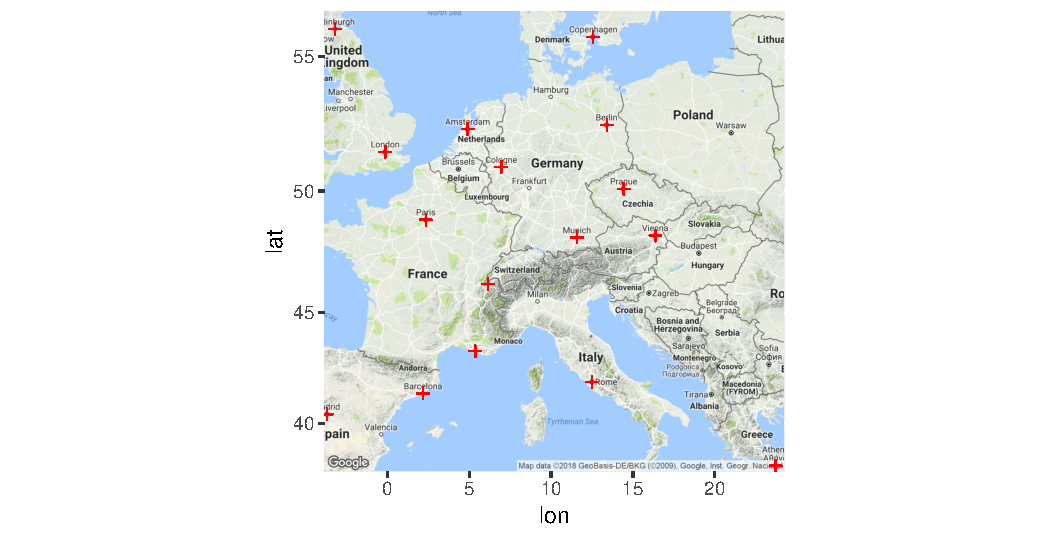
\includegraphics[width=\maxwidth]{figure/unnamed-chunk-19-1} 

\end{knitrout}
  
\end{frame}

\begin{frame}[fragile]{Reminder of data setup}

  \begin{footnotesize}
\begin{knitrout}
\definecolor{shadecolor}{rgb}{0.969, 0.969, 0.969}\color{fgcolor}\begin{kframe}
\begin{alltt}
\hlstd{miners}
\end{alltt}
\begin{verbatim}
## Source: local data frame [24 x 4]
## Groups: Exposure [8]
## 
##    Exposure Severity  Freq proportion
##       <dbl>    <chr> <int>      <dbl>
## 1       5.8     None    98 1.00000000
## 2      15.0     None    51 0.94444444
## 3      21.5     None    34 0.79069767
## 4      27.5     None    35 0.72916667
## 5      33.5     None    32 0.62745098
## 6      39.5     None    23 0.60526316
## 7      46.0     None    12 0.42857143
## 8      51.5     None     4 0.36363636
## 9       5.8 Moderate     0 0.00000000
## 10     15.0 Moderate     2 0.03703704
## # ... with 14 more rows
\end{verbatim}
\end{kframe}
\end{knitrout}
  \end{footnotesize}
\end{frame}


\begin{frame}[fragile]{Creating an ordered factor}
  
  \begin{itemize}
  \item Problem: on plot, \texttt{Severity} categories in \emph{wrong
      order}. 
  \item First we need the different values in  (text) \texttt{Severity}:
    
\begin{knitrout}
\definecolor{shadecolor}{rgb}{0.969, 0.969, 0.969}\color{fgcolor}\begin{kframe}
\begin{alltt}
\hlstd{v}\hlkwb{=}\hlkwd{unique}\hlstd{(miners}\hlopt{$}\hlstd{Severity)}
\hlstd{v}
\end{alltt}
\begin{verbatim}
## [1] "None"     "Moderate" "Severe"
\end{verbatim}
\end{kframe}
\end{knitrout}

\item These are in the right order. Now we make an ordered factor out
  of \texttt{Severity} with these as its levels. Note how it prints out:
  
  {\small
\begin{knitrout}
\definecolor{shadecolor}{rgb}{0.969, 0.969, 0.969}\color{fgcolor}\begin{kframe}
\begin{alltt}
\hlstd{severity.ord}\hlkwb{=}\hlkwd{ordered}\hlstd{(miners}\hlopt{$}\hlstd{Severity,v)}
\hlstd{severity.ord}
\end{alltt}
\begin{verbatim}
##  [1] None     None     None     None     None     None     None    
##  [8] None     Moderate Moderate Moderate Moderate Moderate Moderate
## [15] Moderate Moderate Severe   Severe   Severe   Severe   Severe  
## [22] Severe   Severe   Severe  
## Levels: None < Moderate < Severe
\end{verbatim}
\end{kframe}
\end{knitrout}
}
  \end{itemize}
  
\end{frame}

\begin{frame}[fragile]{Fitting ordered logistic model}

Use function \texttt{polr} from package \texttt{MASS}. Like \texttt{glm}.

{\small
 
\begin{knitrout}
\definecolor{shadecolor}{rgb}{0.969, 0.969, 0.969}\color{fgcolor}\begin{kframe}
\begin{alltt}
\hlkwd{library}\hlstd{(MASS)}
\end{alltt}


{\ttfamily\noindent\itshape\color{messagecolor}{\#\# \\\#\# Attaching package: 'MASS'}}

{\ttfamily\noindent\itshape\color{messagecolor}{\#\# The following object is masked from 'package:dplyr':\\\#\# \\\#\#\ \ \ \  select}}\begin{alltt}
\hlstd{miners.1}\hlkwb{=}\hlkwd{polr}\hlstd{(severity.ord}\hlopt{~}\hlstd{Exposure,}\hlkwc{weights}\hlstd{=Freq,}\hlkwc{data}\hlstd{=miners)}
\end{alltt}
\end{kframe}
\end{knitrout}
}
  
\end{frame}

\begin{frame}[fragile]{Output: not very illuminating}
  
\begin{knitrout}
\definecolor{shadecolor}{rgb}{0.969, 0.969, 0.969}\color{fgcolor}\begin{kframe}
\begin{alltt}
\hlkwd{summary}\hlstd{(miners.1)}
\end{alltt}


{\ttfamily\noindent\itshape\color{messagecolor}{\#\# \\\#\# Re-fitting to get Hessian}}\begin{verbatim}
## Call:
## polr(formula = severity.ord ~ Exposure, data = miners, weights = Freq)
## 
## Coefficients:
##           Value Std. Error t value
## Exposure 0.0959    0.01194   8.034
## 
## Intercepts:
##                 Value   Std. Error t value
## None|Moderate    3.9558  0.4097     9.6558
## Moderate|Severe  4.8690  0.4411    11.0383
## 
## Residual Deviance: 416.9188 
## AIC: 422.9188
\end{verbatim}
\end{kframe}
\end{knitrout}
  
\end{frame}
 
\begin{frame}[fragile]{Does exposure have an effect?}
  
  Fit model without \texttt{Exposure}, and compare
using \texttt{anova}. Note \texttt{1} for model with just intercept:

{\small
\begin{knitrout}
\definecolor{shadecolor}{rgb}{0.969, 0.969, 0.969}\color{fgcolor}\begin{kframe}
\begin{alltt}
\hlstd{miners.0}\hlkwb{=}\hlkwd{polr}\hlstd{(severity.ord}\hlopt{~}\hlnum{1}\hlstd{,}\hlkwc{weights}\hlstd{=Freq,}\hlkwc{data}\hlstd{=miners)}
\hlkwd{anova}\hlstd{(miners.0,miners.1)}
\end{alltt}
\begin{verbatim}
## Likelihood ratio tests of ordinal regression models
## 
## Response: severity.ord
##      Model Resid. df Resid. Dev   Test    Df LR stat. Pr(Chi)
## 1        1       369   505.1621                              
## 2 Exposure       368   416.9188 1 vs 2     1 88.24324       0
\end{verbatim}
\end{kframe}
\end{knitrout}
} 


Exposure definitely has effect on severity of disease. 

  
\end{frame}

\begin{frame}[fragile]{Predicted probabilities}

Make new data frame out of all the exposure values (from original data
frame), and predict from that:

 
\begin{knitrout}
\definecolor{shadecolor}{rgb}{0.969, 0.969, 0.969}\color{fgcolor}\begin{kframe}
\begin{alltt}
\hlstd{miners.new}\hlkwb{=}\hlkwd{data.frame}\hlstd{(}\hlkwc{Exposure}\hlstd{=freqs}\hlopt{$}\hlstd{Exposure)}
\hlstd{pr}\hlkwb{=}\hlkwd{predict}\hlstd{(miners.1,miners.new,}\hlkwc{type}\hlstd{=}\hlstr{"p"}\hlstd{)}
\hlstd{miners.pred}\hlkwb{=}\hlkwd{cbind}\hlstd{(miners.new,pr)}
\hlstd{miners.pred}
\end{alltt}
\begin{verbatim}
##   Exposure      None   Moderate     Severe
## 1      5.8 0.9676920 0.01908912 0.01321885
## 2     15.0 0.9253445 0.04329931 0.03135614
## 3     21.5 0.8692003 0.07385858 0.05694115
## 4     27.5 0.7889290 0.11413004 0.09694093
## 5     33.5 0.6776641 0.16207145 0.16026444
## 6     39.5 0.5418105 0.20484198 0.25334756
## 7     46.0 0.3879962 0.22441555 0.38758828
## 8     51.5 0.2722543 0.21025011 0.51749563
\end{verbatim}
\end{kframe}
\end{knitrout}
 
  
\end{frame}


\begin{frame}[fragile]{Comments}
  
  \begin{itemize}
  \item Model appears to match data: as exposure goes up, prob of None
    goes down, Severe goes up (sharply for high exposure).
  \item Like original data frame, this one nice to look at but
    \emph{not tidy}. We want to make graph, so tidy:
  \item Usual \texttt{gather}:
    
\begin{knitrout}
\definecolor{shadecolor}{rgb}{0.969, 0.969, 0.969}\color{fgcolor}\begin{kframe}
\begin{alltt}
\hlstd{miners.pred} \hlopt
  \hlkwd{gather}\hlstd{(Severity,probability,None}\hlopt{:}\hlstd{Severe)} \hlkwb{->} \hlstd{preds}
\hlkwd{head}\hlstd{(preds)}
\end{alltt}
\begin{verbatim}
##   Exposure Severity probability
## 1      5.8     None   0.9676920
## 2     15.0     None   0.9253445
## 3     21.5     None   0.8692003
## 4     27.5     None   0.7889290
## 5     33.5     None   0.6776641
## 6     39.5     None   0.5418105
\end{verbatim}
\end{kframe}
\end{knitrout}

  \end{itemize}
  
\end{frame}

\begin{frame}[fragile]{Plotting predicted and observed proportions}
  
  Plot:
  \begin{itemize}
  \item predicted probabilities, lines (shown) joining points (not shown)
  \item data, just the points. 
  
  Unfamiliar process: data from two \emph{different} data frames:
  
\begin{knitrout}
\definecolor{shadecolor}{rgb}{0.969, 0.969, 0.969}\color{fgcolor}\begin{kframe}
\begin{alltt}
\hlstd{g}\hlkwb{=}\hlkwd{ggplot}\hlstd{(preds,}\hlkwd{aes}\hlstd{(}\hlkwc{x}\hlstd{=Exposure,}\hlkwc{y}\hlstd{=probability,}
    \hlkwc{colour}\hlstd{=Severity))}\hlopt{+}
  \hlkwd{geom_line}\hlstd{()}\hlopt{+}
  \hlkwd{geom_point}\hlstd{(}\hlkwc{data}\hlstd{=miners,}\hlkwd{aes}\hlstd{(}\hlkwc{y}\hlstd{=proportion))}
\end{alltt}
\end{kframe}
\end{knitrout}

\item Idea: final \texttt{geom\_point} uses data in \texttt{miners}
  rather than \texttt{preds}, $y$-variable for plot is \texttt{prop}
  from that data frame, but $x$-coordinate is \texttt{Exposure}, as it
  was before, and \texttt{colour} is \texttt{Severity} as before. The
  final \texttt{geom\_point} ``inherits'' from the first \texttt{aes}
  as needed.
\item Data conform to fitted relationship pretty well:
  \end{itemize}
  
\end{frame}

\begin{frame}[fragile]{The plot}
  
\begin{knitrout}
\definecolor{shadecolor}{rgb}{0.969, 0.969, 0.969}\color{fgcolor}\begin{kframe}
\begin{alltt}
\hlstd{g}
\end{alltt}
\end{kframe}
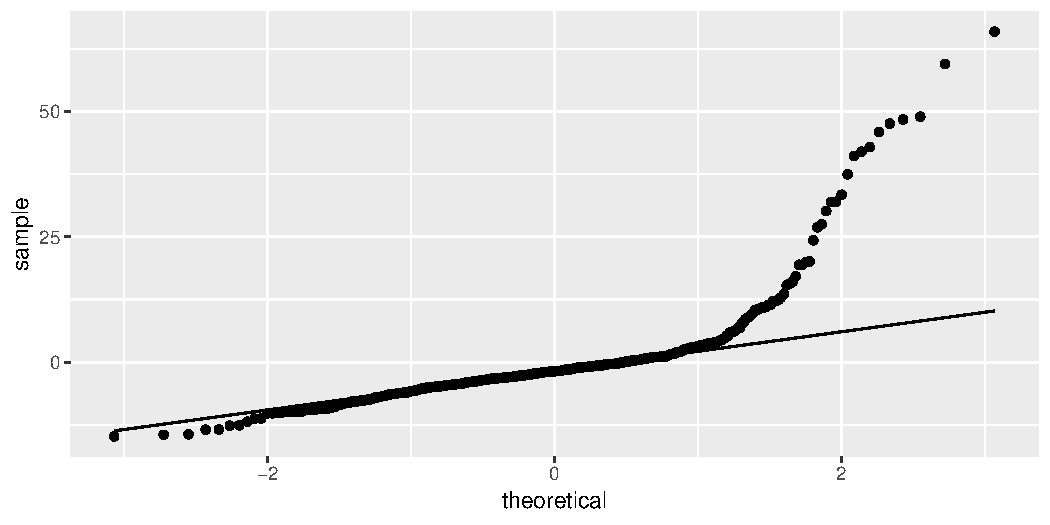
\includegraphics[width=\maxwidth]{figure/unnamed-chunk-29-1} 

\end{knitrout}
  
\end{frame}




% mlogit.pdf

\begin{frame}[fragile]{Unordered responses}

  \begin{itemize}
  \item With unordered (nominal) responses, can use {\em generalized logit}.
  \item Example: 735 people, record age and sex (male 0, female 1), which of 3 brands of some product preferred.
  \item Data in \verb-mlogit.csv- separated by commas (so
    \texttt{read.csv} will work):

 
\begin{knitrout}
\definecolor{shadecolor}{rgb}{0.969, 0.969, 0.969}\color{fgcolor}\begin{kframe}
\begin{alltt}
\hlstd{brandpref}\hlkwb{=}\hlkwd{read.csv}\hlstd{(}\hlstr{"mlogit.csv"}\hlstd{,}\hlkwc{header}\hlstd{=T)}
\hlkwd{head}\hlstd{(brandpref)}
\end{alltt}
\begin{verbatim}
##   brand sex age
## 1     1   0  24
## 2     1   0  26
## 3     1   0  26
## 4     1   1  27
## 5     1   1  27
## 6     3   1  27
\end{verbatim}
\end{kframe}
\end{knitrout}
    

  \end{itemize}

\end{frame}

\begin{frame}[fragile]{Bashing into shape, and fitting model}

  \begin{itemize}
  \item \texttt{sex} and \texttt{brand} not meaningful as numbers, so
    turn into factors
 
\begin{knitrout}
\definecolor{shadecolor}{rgb}{0.969, 0.969, 0.969}\color{fgcolor}\begin{kframe}
\begin{alltt}
\hlstd{brandpref}\hlopt{$}\hlstd{sex}\hlkwb{=}\hlkwd{factor}\hlstd{(brandpref}\hlopt{$}\hlstd{sex)}
\hlstd{brandpref}\hlopt{$}\hlstd{brand}\hlkwb{=}\hlkwd{factor}\hlstd{(brandpref}\hlopt{$}\hlstd{brand)}
\end{alltt}
\end{kframe}
\end{knitrout}
    
  \item We use \texttt{multinom} from package \texttt{nnet}. Works
    like \texttt{polr}.
  \end{itemize}

 
\begin{knitrout}
\definecolor{shadecolor}{rgb}{0.969, 0.969, 0.969}\color{fgcolor}\begin{kframe}
\begin{alltt}
\hlkwd{library}\hlstd{(nnet)}
\hlstd{brands.both}\hlkwb{=}\hlkwd{multinom}\hlstd{(brand}\hlopt{~}\hlstd{age}\hlopt{+}\hlstd{sex,}\hlkwc{data}\hlstd{=brandpref)}
\end{alltt}
\begin{verbatim}
## # weights:  12 (6 variable)
## initial  value 807.480032 
## iter  10 value 702.976983
## final  value 702.970704 
## converged
\end{verbatim}
\end{kframe}
\end{knitrout}
  
\end{frame}

\begin{frame}[fragile]{Do age/sex help predict brand? 1/2}

Fit models without each:

 
\begin{knitrout}
\definecolor{shadecolor}{rgb}{0.969, 0.969, 0.969}\color{fgcolor}\begin{kframe}
\begin{alltt}
\hlstd{brands.age}\hlkwb{=}\hlkwd{multinom}\hlstd{(brand}\hlopt{~}\hlstd{age,}\hlkwc{data}\hlstd{=brandpref)}
\end{alltt}
\begin{verbatim}
## # weights:  9 (4 variable)
## initial  value 807.480032 
## iter  10 value 706.796323
## iter  10 value 706.796322
## final  value 706.796322 
## converged
\end{verbatim}
\begin{alltt}
\hlstd{brands.sex}\hlkwb{=}\hlkwd{multinom}\hlstd{(brand}\hlopt{~}\hlstd{sex,}\hlkwc{data}\hlstd{=brandpref)}
\end{alltt}
\begin{verbatim}
## # weights:  9 (4 variable)
## initial  value 807.480032 
## final  value 791.861266 
## converged
\end{verbatim}
\end{kframe}
\end{knitrout}


  
\end{frame}

\begin{frame}[fragile]{Do age/sex help predict brand? 2/2}

{\footnotesize  
 
\begin{knitrout}
\definecolor{shadecolor}{rgb}{0.969, 0.969, 0.969}\color{fgcolor}\begin{kframe}
\begin{alltt}
\hlkwd{anova}\hlstd{(brands.age,brands.both)}
\end{alltt}
\begin{verbatim}
## Likelihood ratio tests of Multinomial Models
## 
## Response: brand
##       Model Resid. df Resid. Dev   Test    Df LR stat.    Pr(Chi)
## 1       age      1466   1413.593                                 
## 2 age + sex      1464   1405.941 1 vs 2     2 7.651236 0.02180495
\end{verbatim}
\begin{alltt}
\hlkwd{anova}\hlstd{(brands.sex,brands.both)}
\end{alltt}
\begin{verbatim}
## Likelihood ratio tests of Multinomial Models
## 
## Response: brand
##       Model Resid. df Resid. Dev   Test    Df LR stat. Pr(Chi)
## 1       sex      1466   1583.723                              
## 2 age + sex      1464   1405.941 1 vs 2     2 177.7811       0
\end{verbatim}
\end{kframe}
\end{knitrout}
  }
  
\begin{itemize}
\item \texttt{age} definitely significant (second \texttt{anova})
\item \texttt{sex} seems significant also (first \texttt{anova})
\item Keep both.
\end{itemize}
  
  
\end{frame}

\begin{frame}[fragile]{Another way to build model}
  
  \begin{itemize}
  \item Start from model with everything and feed into \texttt{step}:
    
    {\small
\begin{knitrout}
\definecolor{shadecolor}{rgb}{0.969, 0.969, 0.969}\color{fgcolor}\begin{kframe}
\begin{alltt}
\hlkwd{step}\hlstd{(brands.both,}\hlkwc{trace}\hlstd{=}\hlnum{0}\hlstd{)}
\end{alltt}
\begin{verbatim}
## trying - age 
## trying - sex
## Call:
## multinom(formula = brand ~ age + sex, data = brandpref)
## 
## Coefficients:
##   (Intercept)       age      sex1
## 2   -11.77469 0.3682075 0.5238197
## 3   -22.72141 0.6859087 0.4659488
## 
## Residual Deviance: 1405.941 
## AIC: 1417.941
\end{verbatim}
\end{kframe}
\end{knitrout}
}

\item Final model contains both \texttt{age} and \texttt{sex} so neither
could be removed.
  \end{itemize}
  
\end{frame}

\begin{frame}[fragile]{Predictions}

Create data frame with various age and sex. Feed into \texttt{predict}.

{\footnotesize
 
\begin{knitrout}
\definecolor{shadecolor}{rgb}{0.969, 0.969, 0.969}\color{fgcolor}\begin{kframe}
\begin{alltt}
\hlstd{new}\hlkwb{=}\hlkwd{expand.grid}\hlstd{(}\hlkwc{age}\hlstd{=}\hlkwd{c}\hlstd{(}\hlnum{24}\hlstd{,}\hlnum{28}\hlstd{,}\hlnum{32}\hlstd{,}\hlnum{35}\hlstd{,}\hlnum{38}\hlstd{),}\hlkwc{sex}\hlstd{=}\hlkwd{factor}\hlstd{(}\hlnum{0}\hlopt{:}\hlnum{1}\hlstd{))}
\hlstd{pr}\hlkwb{=}\hlkwd{predict}\hlstd{(brands.both,new,}\hlkwc{type}\hlstd{=}\hlstr{"probs"}\hlstd{)}
\hlstd{probs}\hlkwb{=}\hlkwd{cbind}\hlstd{(new,pr)}
\hlstd{probs}
\end{alltt}
\begin{verbatim}
##    age sex          1          2           3
## 1   24   0 0.94795822 0.05022928 0.001812497
## 2   28   0 0.79313204 0.18329690 0.023571058
## 3   32   0 0.40487271 0.40810321 0.187024082
## 4   35   0 0.13057819 0.39724053 0.472181272
## 5   38   0 0.02598163 0.23855071 0.735467663
## 6   24   1 0.91532076 0.08189042 0.002788820
## 7   28   1 0.69561789 0.27143910 0.032943012
## 8   32   1 0.29086347 0.49503135 0.214105181
## 9   35   1 0.08404134 0.43168592 0.484272746
## 10  38   1 0.01623089 0.25162197 0.732147148
\end{verbatim}
\end{kframe}
\end{knitrout}
}

\begin{itemize}
\item Young males (\texttt{sex=0}) prefer brand 1, 
but older males prefer brand 3.
\item Females similar, but like brand 1 less and
  brand 2 more.
\end{itemize}

\end{frame}

\begin{frame}[fragile]{Making a plot}
  
  \begin{itemize}
  \item Plot fitted probability against age, distinguishing brand by
    colour and gender by plotting symbol.
  \item Also join points by lines, and distinguish lines by gender. 
  \item I thought about facetting, but this seems to come out clearer.
  \item First need tidy data frame, by familiar process:
    
\begin{knitrout}
\definecolor{shadecolor}{rgb}{0.969, 0.969, 0.969}\color{fgcolor}\begin{kframe}
\begin{alltt}
\hlstd{probs} \hlopt \hlkwd{gather}\hlstd{(brand,probability,}\hlopt{-}\hlstd{(age}\hlopt{:}\hlstd{sex))} \hlkwb{->} \hlstd{probs.long}
\hlkwd{sample_n}\hlstd{(probs.long,}\hlnum{7}\hlstd{)}
\end{alltt}
\begin{verbatim}
##    age sex brand probability
## 2   28   0     1  0.79313204
## 24  35   0     3  0.47218127
## 27  28   1     3  0.03294301
## 13  32   0     2  0.40810321
## 25  38   0     3  0.73546766
## 7   28   1     1  0.69561789
## 12  28   0     2  0.18329690
\end{verbatim}
\end{kframe}
\end{knitrout}
\item Then (over):
  
  \end{itemize}
  
\end{frame}

\begin{frame}[fragile]{The plot}
  
\begin{knitrout}
\definecolor{shadecolor}{rgb}{0.969, 0.969, 0.969}\color{fgcolor}\begin{kframe}
\begin{alltt}
\hlkwd{ggplot}\hlstd{(probs.long,}\hlkwd{aes}\hlstd{(}\hlkwc{x}\hlstd{=age,}\hlkwc{y}\hlstd{=probability,}
  \hlkwc{colour}\hlstd{=brand,}\hlkwc{shape}\hlstd{=sex))}\hlopt{+}
  \hlkwd{geom_point}\hlstd{()}\hlopt{+}\hlkwd{geom_line}\hlstd{(}\hlkwd{aes}\hlstd{(}\hlkwc{linetype}\hlstd{=sex))}
\end{alltt}
\end{kframe}
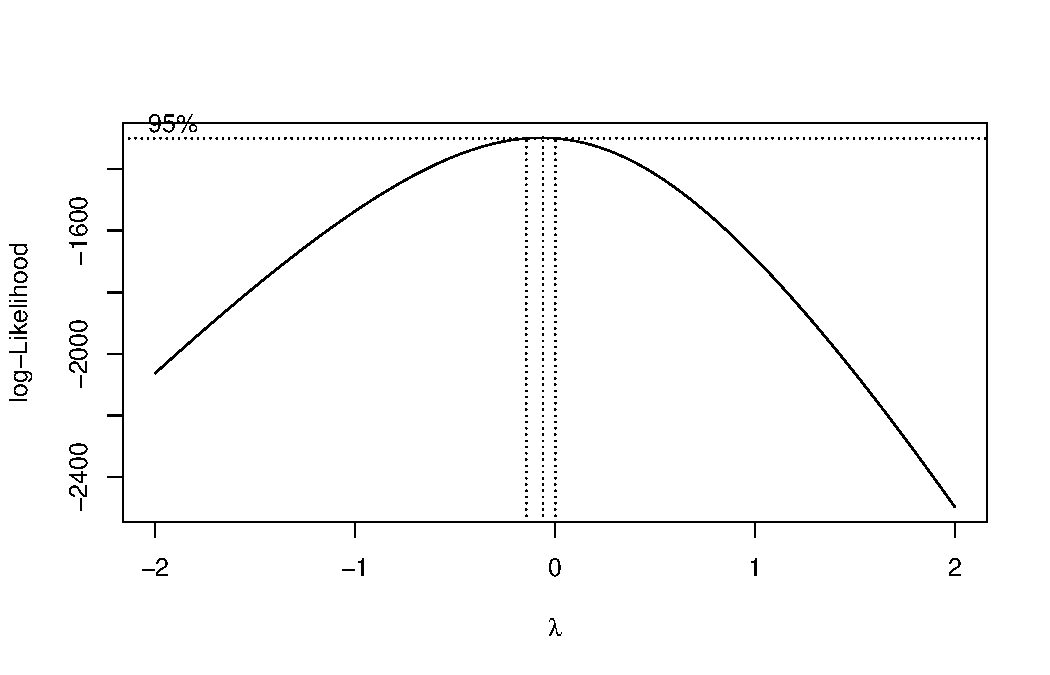
\includegraphics[width=\maxwidth]{figure/unnamed-chunk-38-1} 

\end{knitrout}
\end{frame}


\begin{frame}[fragile]{Digesting the plot}
  
  \begin{itemize}
  \item Brand vs.\ age: younger people (of both genders) prefer brand
    1, but older people (of both genders) prefer brand 3. (Explains
    significant age effect.)
  \item Brand vs.\ sex: females (dashed) like brand 1 less than males
    (solid), like brand 2 more (for all ages). 
    more.
  \item Not much brand difference between genders (solid and dashed
    lines of same colours close), but enough to be significant.
  \item Model didn't include interaction, so modelled effect of gender
    on brand same for each age, modelled effect of age same for each
    gender. 
  \end{itemize}
  
\end{frame}


\begin{frame}[fragile]{Alternative data format}

Summarize all people of same brand preference, same sex, same age on one line of data file with frequency on end:

{
\begin{verbatim}
1 0 24 1
1 0 26 2
1 0 27 4
1 0 28 4
1 0 29 7
1 0 30 3
...
\end{verbatim}
}

Whole data set in 65 lines not 735! But how?
  
\end{frame}

\begin{frame}[fragile]{Getting alternative data format}
  
\begin{knitrout}
\definecolor{shadecolor}{rgb}{0.969, 0.969, 0.969}\color{fgcolor}\begin{kframe}
\begin{alltt}
\hlstd{brandpref} \hlopt
  \hlkwd{group_by}\hlstd{(age,sex,brand)} \hlopt
  \hlkwd{summarize}\hlstd{(}\hlkwc{Freq}\hlstd{=}\hlkwd{n}\hlstd{())} \hlkwb{->} \hlstd{b}
\hlkwd{head}\hlstd{(b)}
\end{alltt}
\begin{verbatim}
## Source: local data frame [6 x 4]
## Groups: age, sex [5]
## 
##     age    sex  brand  Freq
##   <int> <fctr> <fctr> <int>
## 1    24      0      1     1
## 2    26      0      1     2
## 3    27      0      1     4
## 4    27      1      1     4
## 5    27      1      3     1
## 6    28      0      1     4
\end{verbatim}
\end{kframe}
\end{knitrout}
  
\end{frame}



\begin{frame}[fragile]{Fitting models, almost the same}

  \begin{itemize}
  \item Just have to remember \texttt{weights} to incorporate
frequencies.
\item Otherwise \texttt{multinom} assumes you have just 1 obs
on each line!
\item Again turn (numerical) \texttt{sex} and \texttt{brand} into factors:
{\small
 
\begin{knitrout}
\definecolor{shadecolor}{rgb}{0.969, 0.969, 0.969}\color{fgcolor}\begin{kframe}
\begin{alltt}
\hlstd{b}\hlopt{$}\hlstd{sex}\hlkwb{=}\hlkwd{factor}\hlstd{(b}\hlopt{$}\hlstd{sex)}
\hlstd{b}\hlopt{$}\hlstd{brand}\hlkwb{=}\hlkwd{factor}\hlstd{(b}\hlopt{$}\hlstd{brand)}
\hlstd{b.both}\hlkwb{=}\hlkwd{multinom}\hlstd{(brand}\hlopt{~}\hlstd{age}\hlopt{+}\hlstd{sex,}\hlkwc{data}\hlstd{=b,}\hlkwc{weights}\hlstd{=Freq)}
\end{alltt}
\begin{verbatim}
## # weights:  12 (6 variable)
## initial  value 807.480032 
## iter  10 value 702.976983
## final  value 702.970704 
## converged
\end{verbatim}
\begin{alltt}
\hlstd{b.age}\hlkwb{=}\hlkwd{multinom}\hlstd{(brand}\hlopt{~}\hlstd{age,}\hlkwc{data}\hlstd{=b,}\hlkwc{weights}\hlstd{=Freq)}
\end{alltt}
\begin{verbatim}
## # weights:  9 (4 variable)
## initial  value 807.480032 
## iter  10 value 706.796323
## iter  10 value 706.796322
## final  value 706.796322 
## converged
\end{verbatim}
\end{kframe}
\end{knitrout}
}  

  \end{itemize}

  
\end{frame}

\begin{frame}[fragile]{P-value for \texttt{sex} identical}
  
{\small  
 
\begin{knitrout}
\definecolor{shadecolor}{rgb}{0.969, 0.969, 0.969}\color{fgcolor}\begin{kframe}
\begin{alltt}
\hlkwd{anova}\hlstd{(b.age,b.both)}
\end{alltt}
\begin{verbatim}
## Likelihood ratio tests of Multinomial Models
## 
## Response: brand
##       Model Resid. df Resid. Dev   Test    Df LR stat.    Pr(Chi)
## 1       age       126   1413.593                                 
## 2 age + sex       124   1405.941 1 vs 2     2 7.651236 0.02180495
\end{verbatim}
\end{kframe}
\end{knitrout}
}

Same P-value as before, so we haven't changed anything important.
  
\end{frame}

\begin{frame}[fragile]{Including data on plot}
  
  \begin{itemize}
  \item Everyone's age given as whole
    number, so maybe not too many different ages with sensible amount
    of data at each:
    
    \begin{footnotesize}
\begin{knitrout}
\definecolor{shadecolor}{rgb}{0.969, 0.969, 0.969}\color{fgcolor}\begin{kframe}
\begin{alltt}
\hlstd{b} \hlopt \hlkwd{group_by}\hlstd{(age)} \hlopt
  \hlkwd{summarize}\hlstd{(}\hlkwc{total}\hlstd{=}\hlkwd{sum}\hlstd{(Freq))}
\end{alltt}
\begin{verbatim}
## # A tibble: 14 × 2
##      age total
##    <int> <int>
## 1     24     1
## 2     26     2
## 3     27     9
## 4     28    15
## 5     29    19
## 6     30    23
## 7     31    40
## 8     32   333
## 9     33    55
## 10    34    64
## 11    35    35
## 12    36    85
## 13    37    22
## 14    38    32
\end{verbatim}
\end{kframe}
\end{knitrout}
%$ %$
    \end{footnotesize}
    
   
  \end{itemize}
  
\end{frame}

\begin{frame}[fragile]{Comments and next}
  \begin{itemize}
  \item Not great (especially at low end), but live with it.
  \item Need proportions of frequencies in each brand for each
    age-gender combination. Mimic what we did for miners:
\begin{knitrout}
\definecolor{shadecolor}{rgb}{0.969, 0.969, 0.969}\color{fgcolor}\begin{kframe}
\begin{alltt}
\hlstd{b} \hlopt
  \hlkwd{group_by}\hlstd{(age,sex)} \hlopt
  \hlkwd{mutate}\hlstd{(}\hlkwc{proportion}\hlstd{=}\hlkwd{prop.table}\hlstd{(Freq))} \hlkwb{->} \hlstd{brands}
\end{alltt}
\end{kframe}
\end{knitrout}
  \end{itemize}
\end{frame}

\begin{frame}[fragile]{Checking proportions for age 32}
  
  
\begin{knitrout}
\definecolor{shadecolor}{rgb}{0.969, 0.969, 0.969}\color{fgcolor}\begin{kframe}
\begin{alltt}
\hlstd{brands} \hlopt \hlkwd{filter}\hlstd{(age}\hlopt{==}\hlnum{32}\hlstd{)}
\end{alltt}
\begin{verbatim}
## Source: local data frame [6 x 5]
## Groups: age, sex [2]
## 
##     age    sex  brand  Freq proportion
##   <int> <fctr> <fctr> <int>      <dbl>
## 1    32      0      1    48  0.4067797
## 2    32      0      2    51  0.4322034
## 3    32      0      3    19  0.1610169
## 4    32      1      1    62  0.2883721
## 5    32      1      2   117  0.5441860
## 6    32      1      3    36  0.1674419
\end{verbatim}
\end{kframe}
\end{knitrout}

\begin{itemize}
\item First three proportions (males) add up to 1.
\item Last three proportions (females) add up to 1.
\item So looks like proportions of right thing.
  
\end{itemize}
  
\end{frame}

\begin{frame}[fragile]{Attempting plot}
  
  \begin{itemize}
  \item Take code from previous plot and:
    \begin{itemize}
    \item remove \texttt{geom\_point} for fitted values
    \item add \texttt{geom\_point} with correct \texttt{data=} and
      \texttt{aes} to plot data.
    \end{itemize}
    
\begin{knitrout}
\definecolor{shadecolor}{rgb}{0.969, 0.969, 0.969}\color{fgcolor}\begin{kframe}
\begin{alltt}
\hlstd{g}\hlkwb{=}\hlkwd{ggplot}\hlstd{(probs.long,}\hlkwd{aes}\hlstd{(}\hlkwc{x}\hlstd{=age,}\hlkwc{y}\hlstd{=probability,}
  \hlkwc{colour}\hlstd{=brand,}\hlkwc{shape}\hlstd{=sex))}\hlopt{+}
  \hlkwd{geom_line}\hlstd{(}\hlkwd{aes}\hlstd{(}\hlkwc{linetype}\hlstd{=sex))}\hlopt{+}
  \hlkwd{geom_point}\hlstd{(}\hlkwc{data}\hlstd{=brands,}\hlkwd{aes}\hlstd{(}\hlkwc{y}\hlstd{=proportion))}
\end{alltt}
\end{kframe}
\end{knitrout}

\item Data seem to correspond more or less to fitted curves:
  \end{itemize}
  
\end{frame}

\begin{frame}[fragile]{The plot}
  
\begin{knitrout}
\definecolor{shadecolor}{rgb}{0.969, 0.969, 0.969}\color{fgcolor}\begin{kframe}
\begin{alltt}
\hlstd{g}
\end{alltt}
\end{kframe}
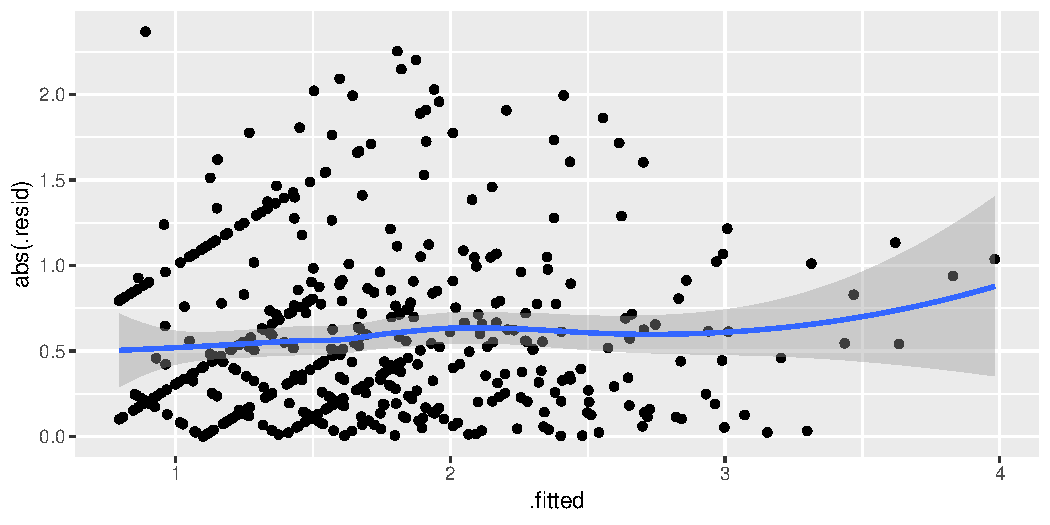
\includegraphics[width=\maxwidth]{figure/unnamed-chunk-45-1} 

\end{knitrout}
\end{frame}

\begin{frame}[fragile]{Trying interaction between age and gender}
  
  \begin{scriptsize}
\begin{knitrout}
\definecolor{shadecolor}{rgb}{0.969, 0.969, 0.969}\color{fgcolor}\begin{kframe}
\begin{alltt}
\hlstd{b.int}\hlkwb{=}\hlkwd{update}\hlstd{(b.both,.}\hlopt{~}\hlstd{.}\hlopt{+}\hlstd{age}\hlopt{:}\hlstd{sex)}
\end{alltt}
\begin{verbatim}
## # weights:  15 (8 variable)
## initial  value 807.480032 
## iter  10 value 704.811229
## iter  20 value 702.582802
## final  value 702.582761 
## converged
\end{verbatim}
\begin{alltt}
\hlkwd{anova}\hlstd{(b.both,b.int)}
\end{alltt}
\begin{verbatim}
## Likelihood ratio tests of Multinomial Models
## 
## Response: brand
##                 Model Resid. df Resid. Dev   Test    Df  LR stat.  Pr(Chi)
## 1           age + sex       124   1405.941                                
## 2 age + sex + age:sex       122   1405.166 1 vs 2     2 0.7758861 0.678451
\end{verbatim}
\end{kframe}
\end{knitrout}
    
  \end{scriptsize}

  \begin{itemize}
  \item No evidence that effect of age on brand preference differs for
    the two genders.
  \end{itemize}
\end{frame}

\section{Survival analysis}
\frame{\sectionpage}

\begin{frame}[fragile]{Survival analysis}

  \begin{itemize}
  \item So far, have seen:
    \begin{itemize}
    \item response variable counted or measured (regression)
    \item response variable categorized (logistic regression)
    \end{itemize}
    and have predicted response from explanatory variables.
  \item But what if response is time until event (eg.\ time of
    survival after surgery)?
  \item Additional complication: event might not have happened at end of study (eg.\ patient still alive). But knowing that patient has ``not died yet'' presumably informative. Such data called {\em censored}. 
  \item Enter {\em survival analysis}, in particular the ``Cox proportional hazards model''. 
  \item Explanatory variables in this context often called {\em covariates}.
  \end{itemize}

\end{frame}

\begin{frame}[fragile]{Example: still dancing?}

  \begin{itemize}
  \item 12 women who have just started taking dancing lessons are
    followed for up to a year, to see whether they are still taking
    dancing lessons, or have quit. The ``event'' here is ``quit''.
  \item This might depend on:
    \begin{itemize}
    \item a treatment (visit to a dance competition)
    \item woman's age (at start of study).
    \end{itemize}
  \item Data:

{\scriptsize
\begin{verbatim}
Months  Quit   Treatment Age
   1      1        0      16
   2      1        0      24
   2      1        0      18
   3      0        0      27
   4      1        0      25
   7      1        1      26
   8      1        1      36
  10      1        1      38
  10      0        1      45
  12      1        1      47
\end{verbatim}
}

  \end{itemize}
  
\end{frame}
 
\begin{frame}[fragile]{About the data}

  \begin{itemize}
  \item \verb-months- and \verb-quit- are kind of combined response:
    \begin{itemize}
    \item  \verb-Months- is number of months a woman was actually observed dancing
    \item \verb-quit- is 1 if woman quit, 0 if still dancing at end of study.
    \end{itemize}
  \item Treatment is 1 if woman went to dance competition, 0 otherwise.
  \item Fit model and see whether \texttt{Age} or \texttt{Treatment}
    have effect on survival.
  \item Want to do predictions for probabilities of still dancing as
    they depend on whatever is significant, and draw plot.
\end{itemize}
\end{frame}


\begin{frame}[fragile]{The code}

  \begin{itemize}
  \item First, call in \texttt{survival} and \texttt{survminer}
    packages, read data and make combined response:
 
\begin{knitrout}
\definecolor{shadecolor}{rgb}{0.969, 0.969, 0.969}\color{fgcolor}\begin{kframe}
\begin{alltt}
\hlkwd{library}\hlstd{(survival)}
\hlkwd{library}\hlstd{(survminer)}
\end{alltt}


{\ttfamily\noindent\itshape\color{messagecolor}{\#\# Loading required package: ggplot2}}\begin{alltt}
\hlstd{dance}\hlkwb{=}\hlkwd{read.table}\hlstd{(}\hlstr{"dancing.txt"}\hlstd{,}\hlkwc{header}\hlstd{=T)}
\hlkwd{attach}\hlstd{(dance)}
\hlstd{mth}\hlkwb{=}\hlkwd{Surv}\hlstd{(Months,Quit)}
\hlstd{mth}
\end{alltt}
\begin{verbatim}
##  [1]  1   2   2   3+  4   5  11   7   8  10  10+ 12
\end{verbatim}
\end{kframe}
\end{knitrout}

    
  \item Then fit model, predicting \texttt{mth} from explanatories:

 
\begin{knitrout}
\definecolor{shadecolor}{rgb}{0.969, 0.969, 0.969}\color{fgcolor}\begin{kframe}
\begin{alltt}
\hlstd{dance.1}\hlkwb{=}\hlkwd{coxph}\hlstd{(mth}\hlopt{~}\hlstd{Treatment}\hlopt{+}\hlstd{Age)}
\end{alltt}
\end{kframe}
\end{knitrout}


  \end{itemize}

\end{frame}

\begin{frame}[fragile]{Output looks a lot like regression}

{\footnotesize
 
\begin{knitrout}
\definecolor{shadecolor}{rgb}{0.969, 0.969, 0.969}\color{fgcolor}\begin{kframe}
\begin{alltt}
\hlkwd{summary}\hlstd{(dance.1)}
\end{alltt}
\begin{verbatim}
## Call:
## coxph(formula = mth ~ Treatment + Age)
## 
##   n= 12, number of events= 10 
## 
##               coef exp(coef) se(coef)      z Pr(>|z|)  
## Treatment -4.44915   0.01169  2.60929 -1.705   0.0882 .
## Age       -0.36619   0.69337  0.15381 -2.381   0.0173 *
## ---
## Signif. codes:  0 '***' 0.001 '**' 0.01 '*' 0.05 '.' 0.1 ' ' 1
## 
##           exp(coef) exp(-coef) lower .95 upper .95
## Treatment   0.01169     85.554 7.026e-05    1.9444
## Age         0.69337      1.442 5.129e-01    0.9373
## 
## Concordance= 0.964  (se = 0.125 )
## Rsquare= 0.836   (max possible= 0.938 )
## Likelihood ratio test= 21.68  on 2 df,   p=1.956e-05
## Wald test            = 5.67  on 2 df,   p=0.0587
## Score (logrank) test = 14.75  on 2 df,   p=0.0006274
\end{verbatim}
\end{kframe}
\end{knitrout}
}
  
\end{frame}

\begin{frame}[fragile]{Conclusions}

  \begin{itemize}
  \item Use $\alpha=0.10$ here since not much data.
  \item Three tests at bottom like global F-test. Consensus that
    something predicts survival time (whether or not dancer quit and how
    long it took).
  \item \texttt{Age} (definitely), \texttt{Treatment} (marginally) both
    predict survival time.
  \end{itemize}


  
\end{frame}

\begin{frame}[fragile]{Model checking}
  
  \begin{itemize}
  \item With regression, usually plot residuals against fitted values.
  \item Not quite same here (nonlinear model), but ``martingale
    residuals'' should have no pattern vs.\ ``linear predictor''.
  \item \texttt{ggcoxdiagnostics} from package \texttt{survminer}
    makes plot, to which we add smooth. If smooth trend more or less
    straight across, model OK. 
  \item Martingale residuals can go very negative, so won't always
    look normal.
  \end{itemize}
  
\end{frame}

\begin{frame}[fragile]{Martingale residual plot for dance data}
  
\begin{knitrout}
\definecolor{shadecolor}{rgb}{0.969, 0.969, 0.969}\color{fgcolor}\begin{kframe}
\begin{alltt}
\hlkwd{ggcoxdiagnostics}\hlstd{(dance.1)}\hlopt{+}\hlkwd{geom_smooth}\hlstd{(}\hlkwc{se}\hlstd{=F)}
\end{alltt}


{\ttfamily\noindent\itshape\color{messagecolor}{\#\# `geom\_smooth()` using method = 'loess'}}\end{kframe}
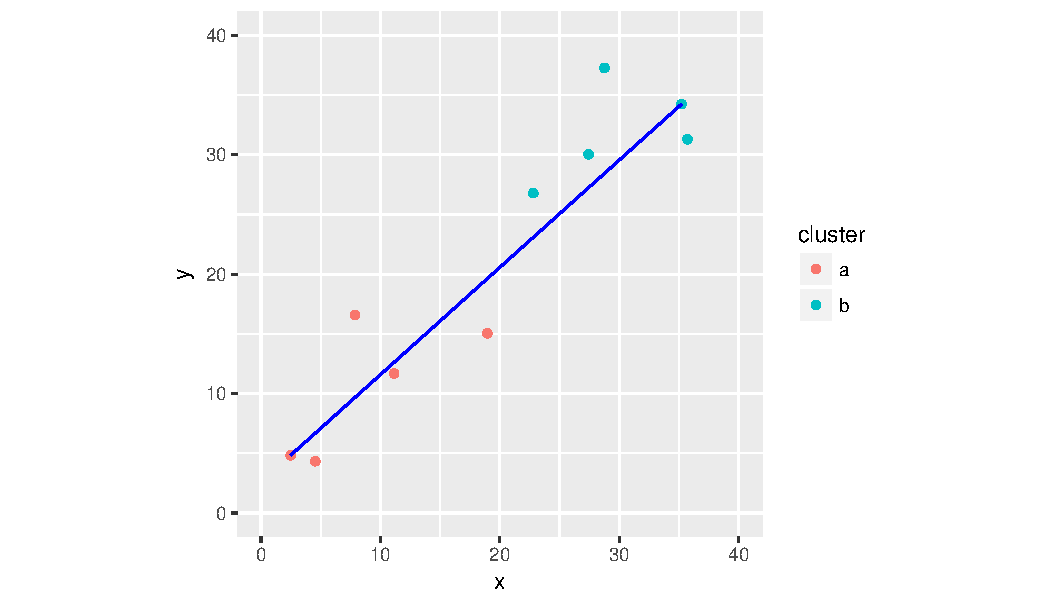
\includegraphics[width=\maxwidth]{figure/unnamed-chunk-4-1} 

\end{knitrout}

This looks good (with only 12 points).
  
\end{frame}

\begin{frame}[fragile]{Predicted survival probs}

The function we use is called
\texttt{survfit}, though actually works rather like
\texttt{predict}. 

First create a data frame of values to predict from. We'll do all
combos of ages 20 and 40, treatment and not, using
\texttt{expand.grid} to get all the combos:

 
\begin{knitrout}
\definecolor{shadecolor}{rgb}{0.969, 0.969, 0.969}\color{fgcolor}\begin{kframe}
\begin{alltt}
\hlstd{dance.new}\hlkwb{=}\hlkwd{expand.grid}\hlstd{(}\hlkwc{Treatment}\hlstd{=}\hlkwd{c}\hlstd{(}\hlnum{0}\hlstd{,}\hlnum{1}\hlstd{),}\hlkwc{Age}\hlstd{=}\hlkwd{c}\hlstd{(}\hlnum{20}\hlstd{,}\hlnum{40}\hlstd{))}
\hlstd{dance.new}
\end{alltt}
\begin{verbatim}
##   Treatment Age
## 1         0  20
## 2         1  20
## 3         0  40
## 4         1  40
\end{verbatim}
\end{kframe}
\end{knitrout}


Then run \texttt{survfit}. Actual predictions via \texttt{summary}
(next page):

 
\begin{knitrout}
\definecolor{shadecolor}{rgb}{0.969, 0.969, 0.969}\color{fgcolor}\begin{kframe}
\begin{alltt}
\hlstd{s}\hlkwb{=}\hlkwd{survfit}\hlstd{(dance.1,}\hlkwc{newdata}\hlstd{=dance.new)}
\end{alltt}
\end{kframe}
\end{knitrout}


\end{frame}

\begin{frame}[fragile]{The predictions}

One prediction \emph{for each time} for each combo of age and treatment:

{\footnotesize
 
\begin{knitrout}
\definecolor{shadecolor}{rgb}{0.969, 0.969, 0.969}\color{fgcolor}\begin{kframe}
\begin{alltt}
\hlkwd{summary}\hlstd{(s)}
\end{alltt}
\begin{verbatim}
## Call: survfit(formula = dance.1, newdata = dance.new)
## 
##  time n.risk n.event survival1 survival2 survival3 survival4
##     1     12       1  8.76e-01  9.98e-01  1.00e+00     1.000
##     2     11       2  3.99e-01  9.89e-01  9.99e-01     1.000
##     4      8       1  1.24e-01  9.76e-01  9.99e-01     1.000
##     5      7       1  2.93e-02  9.60e-01  9.98e-01     1.000
##     7      6       1 2.96e-323  1.70e-04  6.13e-01     0.994
##     8      5       1  0.00e+00  1.35e-98  2.99e-06     0.862
##    10      4       1  0.00e+00  0.00e+00  3.61e-20     0.593
##    11      2       1  0.00e+00  0.00e+00  0.00e+00     0.000
##    12      1       1  0.00e+00  0.00e+00  0.00e+00     0.000
\end{verbatim}
\begin{alltt}
\hlkwd{t}\hlstd{(dance.new)}
\end{alltt}
\begin{verbatim}
##           [,1] [,2] [,3] [,4]
## Treatment    0    1    0    1
## Age         20   20   40   40
\end{verbatim}
\end{kframe}
\end{knitrout}
}

\texttt{dance.new} transposed (flipped around) shows which combo the
four lists of survival probabilities belong to.
  
\end{frame}

\begin{frame}[fragile]{Conclusions from predicted probs}

  \begin{itemize}
  \item Older women more likely to be still dancing than younger women
    (compare ``profiles'' for same treatment group).
  \item Effect of treatment seems to be to increase prob of still dancing (compare ``profiles'' for same age for treatment group vs.\ not)
  \item Would be nice to see this on a graph.
  \end{itemize}
  
\end{frame}

\begin{frame}[fragile]{Plotting survival probabilities}
  
  \begin{itemize}
  \item I like package \texttt{survminer} with function \texttt{ggsurvplot}:
    
\begin{knitrout}
\definecolor{shadecolor}{rgb}{0.969, 0.969, 0.969}\color{fgcolor}\begin{kframe}
\begin{alltt}
\hlkwd{library}\hlstd{(survminer)}
\hlstd{g}\hlkwb{=}\hlkwd{ggsurvplot}\hlstd{(s)}
\end{alltt}
\end{kframe}
\end{knitrout}
  \end{itemize}
  
\end{frame}

\begin{frame}[fragile]{The plot}
  
\begin{knitrout}
\definecolor{shadecolor}{rgb}{0.969, 0.969, 0.969}\color{fgcolor}\begin{kframe}
\begin{alltt}
\hlstd{g}
\end{alltt}
\end{kframe}
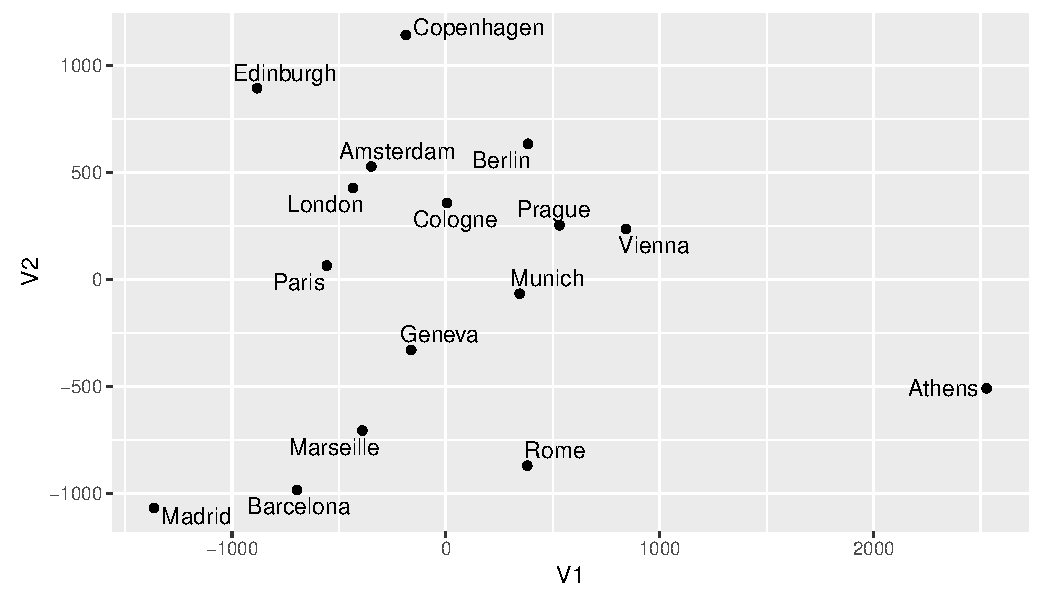
\includegraphics[width=\maxwidth]{figure/unnamed-chunk-9-1} 

\end{knitrout}

\begin{small}
\begin{tabular}{rrr}
  Stratum& Age& Treatment \\
  \hline
  1 & 20 & no\\
  2 & 20 & yes\\
  3 & 40 & no\\
  4 & 40 & yes\\
  \hline
\end{tabular}  
\end{small}
  
\end{frame}

\begin{frame}[fragile]{Discussion}
%  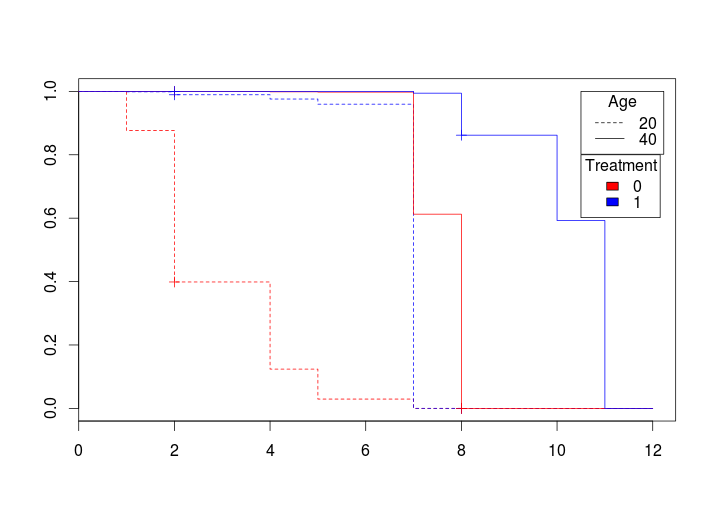
\includegraphics[width=2in]{dance-2}

  
  \begin{itemize}
  \item Survivor curve farther to the right is better (better chance
    of surviving longer).
  \item Best is age 40 with treatment, worst age 20 without.
  \item Appears to be:
    \begin{itemize}
    \item age effect (40 better than 20)
    \item treatment effect (treatment better than not)
    \end{itemize}
  \item In analysis, treatment effect only marginally significant.
  \end{itemize}

\end{frame}



\begin{frame}[fragile]{A more realistic example: lung cancer}


\begin{itemize}
\item When you
load in an R package, get data sets to illustrate 
functions in the package. 
\item One such is \texttt{lung}. Data
set measuring survival in patients with advanced lung cancer. 
\item Along with survival time, number of ``performance scores''
  included, measuring how well patients can perform daily
  activities.
\item Sometimes high good, but sometimes bad!
\item Variables below,
  from the help file data set (\texttt{?lung}).
\end{itemize}
\end{frame}

\begin{frame}[fragile]{The variables}

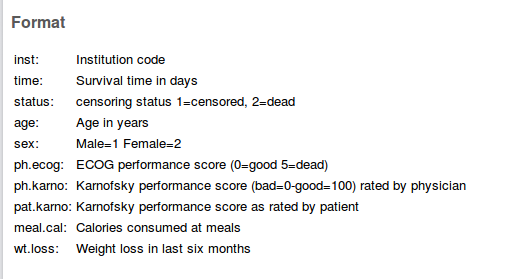
\includegraphics[width=\textwidth]{lung-cancer-data}  

  
\end{frame}

\begin{frame}[fragile]{Uh oh, missing values}
  
  \begin{scriptsize}
\begin{knitrout}
\definecolor{shadecolor}{rgb}{0.969, 0.969, 0.969}\color{fgcolor}\begin{kframe}
\begin{alltt}
\hlkwd{head}\hlstd{(lung,}\hlnum{12}\hlstd{)}
\end{alltt}
\begin{verbatim}
##    inst time status age sex ph.ecog ph.karno pat.karno meal.cal wt.loss
## 1     3  306      2  74   1       1       90       100     1175      NA
## 2     3  455      2  68   1       0       90        90     1225      15
## 3     3 1010      1  56   1       0       90        90       NA      15
## 4     5  210      2  57   1       1       90        60     1150      11
## 5     1  883      2  60   1       0      100        90       NA       0
## 6    12 1022      1  74   1       1       50        80      513       0
## 7     7  310      2  68   2       2       70        60      384      10
## 8    11  361      2  71   2       2       60        80      538       1
## 9     1  218      2  53   1       1       70        80      825      16
## 10    7  166      2  61   1       2       70        70      271      34
## 11    6  170      2  57   1       1       80        80     1025      27
## 12   16  654      2  68   2       2       70        70       NA      23
\end{verbatim}
\end{kframe}
\end{knitrout}
  \end{scriptsize}
  
\end{frame}

\begin{frame}[fragile]{Remove any obs with any missing values}
  

  
\begin{knitrout}
\definecolor{shadecolor}{rgb}{0.969, 0.969, 0.969}\color{fgcolor}\begin{kframe}
\begin{alltt}
\hlstd{lung} \hlopt \hlkwd{na.omit}\hlstd{()} \hlkwb{->} \hlstd{lung.complete}
\hlstd{lung.complete} \hlopt \hlkwd{select}\hlstd{(meal.cal}\hlopt{:}\hlstd{wt.loss)} \hlopt \hlkwd{head}\hlstd{(}\hlnum{12}\hlstd{)}
\end{alltt}
\begin{verbatim}
##    meal.cal wt.loss
## 2      1225      15
## 4      1150      11
## 6       513       0
## 7       384      10
## 8       538       1
## 9       825      16
## 10      271      34
## 11     1025      27
## 15     2600      60
## 17     1150      -5
## 18     1025      22
## 19      238      10
\end{verbatim}
\end{kframe}
\end{knitrout}
  
\end{frame}

\begin{frame}[fragile]{Model 1: use everything}

{\scriptsize  
 
\begin{knitrout}
\definecolor{shadecolor}{rgb}{0.969, 0.969, 0.969}\color{fgcolor}\begin{kframe}
\begin{alltt}
\hlkwd{head}\hlstd{(lung.complete)}
\end{alltt}
\begin{verbatim}
##   inst time status age sex ph.ecog ph.karno pat.karno meal.cal wt.loss
## 2    3  455      2  68   1       0       90        90     1225      15
## 4    5  210      2  57   1       1       90        60     1150      11
## 6   12 1022      1  74   1       1       50        80      513       0
## 7    7  310      2  68   2       2       70        60      384      10
## 8   11  361      2  71   2       2       60        80      538       1
## 9    1  218      2  53   1       1       70        80      825      16
\end{verbatim}
\end{kframe}
\end{knitrout}

}

\begin{knitrout}
\definecolor{shadecolor}{rgb}{0.969, 0.969, 0.969}\color{fgcolor}\begin{kframe}
\begin{alltt}
\hlstd{resp}\hlkwb{=}\hlkwd{with}\hlstd{(lung.complete,}\hlkwd{Surv}\hlstd{(time,status}\hlopt{==}\hlnum{2}\hlstd{))}
\hlstd{lung.1}\hlkwb{=}\hlkwd{coxph}\hlstd{(resp}\hlopt{~}\hlstd{age}\hlopt{+}\hlstd{sex}\hlopt{+}\hlstd{ph.ecog}\hlopt{+}\hlstd{ph.karno}\hlopt{+}\hlstd{pat.karno}\hlopt{+}
               \hlstd{meal.cal}\hlopt{+}\hlstd{wt.loss,}\hlkwc{data}\hlstd{=lung.complete)}
\end{alltt}
\end{kframe}
\end{knitrout}


\end{frame}

\begin{frame}[fragile]{\texttt{summary} of model 1: too tiny to see!}

{\tiny  
 
\begin{knitrout}
\definecolor{shadecolor}{rgb}{0.969, 0.969, 0.969}\color{fgcolor}\begin{kframe}
\begin{alltt}
\hlkwd{summary}\hlstd{(lung.1)}
\end{alltt}
\begin{verbatim}
## Call:
## coxph(formula = resp ~ age + sex + ph.ecog + ph.karno + pat.karno + 
##     meal.cal + wt.loss, data = lung.complete)
## 
##   n= 167, number of events= 120 
## 
##                 coef  exp(coef)   se(coef)      z Pr(>|z|)   
## age        1.080e-02  1.011e+00  1.160e-02  0.931  0.35168   
## sex       -5.536e-01  5.749e-01  2.016e-01 -2.746  0.00603 **
## ph.ecog    7.395e-01  2.095e+00  2.250e-01  3.287  0.00101 **
## ph.karno   2.244e-02  1.023e+00  1.123e-02  1.998  0.04575 * 
## pat.karno -1.207e-02  9.880e-01  8.116e-03 -1.488  0.13685   
## meal.cal   2.835e-05  1.000e+00  2.594e-04  0.109  0.91298   
## wt.loss   -1.420e-02  9.859e-01  7.766e-03 -1.828  0.06748 . 
## ---
## Signif. codes:  0 '***' 0.001 '**' 0.01 '*' 0.05 '.' 0.1 ' ' 1
## 
##           exp(coef) exp(-coef) lower .95 upper .95
## age          1.0109     0.9893    0.9881    1.0341
## sex          0.5749     1.7395    0.3872    0.8534
## ph.ecog      2.0950     0.4773    1.3479    3.2560
## ph.karno     1.0227     0.9778    1.0004    1.0455
## pat.karno    0.9880     1.0121    0.9724    1.0038
## meal.cal     1.0000     1.0000    0.9995    1.0005
## wt.loss      0.9859     1.0143    0.9710    1.0010
## 
## Concordance= 0.653  (se = 0.031 )
## Rsquare= 0.155   (max possible= 0.998 )
## Likelihood ratio test= 28.16  on 7 df,   p=0.0002053
## Wald test            = 27.5  on 7 df,   p=0.0002711
## Score (logrank) test = 28.31  on 7 df,   p=0.0001929
\end{verbatim}
\end{kframe}
\end{knitrout}
}

\end{frame}

\begin{frame}[fragile]{Overall significance}
 

The three tests of overall significance:

 
\begin{knitrout}
\definecolor{shadecolor}{rgb}{0.969, 0.969, 0.969}\color{fgcolor}\begin{kframe}
\begin{alltt}
\hlstd{s}\hlkwb{=}\hlkwd{summary}\hlstd{(lung.1)}
\hlkwd{rbind}\hlstd{(s}\hlopt{$}\hlstd{logtest,s}\hlopt{$}\hlstd{waldtest,s}\hlopt{$}\hlstd{sctest)}
\end{alltt}
\begin{verbatim}
##          test df       pvalue
## [1,] 28.16471  7 0.0002052811
## [2,] 27.50000  7 0.0002711044
## [3,] 28.31331  7 0.0001929209
\end{verbatim}
\end{kframe}
\end{knitrout}

All strongly significant. \emph{Something} predicts survival.  

\end{frame}

\begin{frame}[fragile]{Coefficients for model 1}
  
{\footnotesize  
 
\begin{knitrout}
\definecolor{shadecolor}{rgb}{0.969, 0.969, 0.969}\color{fgcolor}\begin{kframe}
\begin{alltt}
\hlstd{s}\hlopt{$}\hlstd{coefficients}
\end{alltt}
\begin{verbatim}
##                    coef exp(coef)     se(coef)          z    Pr(>|z|)
## age        1.080338e-02 1.0108619 0.0115998987  0.9313337 0.351681000
## sex       -5.536181e-01 0.5748661 0.2015855722 -2.7463179 0.006026834
## ph.ecog    7.395321e-01 2.0949551 0.2249867714  3.2870027 0.001012598
## ph.karno   2.243783e-02 1.0226914 0.0112317607  1.9977122 0.045747870
## pat.karno -1.207386e-02 0.9879987 0.0081162309 -1.4876191 0.136851382
## meal.cal   2.834683e-05 1.0000283 0.0002593848  0.1092848 0.912976585
## wt.loss   -1.420024e-02 0.9859001 0.0077662937 -1.8284443 0.067482902
\end{verbatim}
\end{kframe}
\end{knitrout}
}

  \begin{itemize}
  \item Model as a whole significant (strongly)
  \item \texttt{sex} and
\texttt{ph.ecog} definitely significant
\item \texttt{age}, \texttt{pat.karno} and
\texttt{meal.cal} definitely not
\item  others in
between
\item Take out the three variables that are definitely not
significant, and try again.
  \end{itemize}


\end{frame}


\begin{frame}[fragile]{Model 2 (edited)}

{\footnotesize  
 
\begin{knitrout}
\definecolor{shadecolor}{rgb}{0.969, 0.969, 0.969}\color{fgcolor}\begin{kframe}
\begin{alltt}
\hlstd{lung.2}\hlkwb{=}\hlkwd{update}\hlstd{(lung.1,.}\hlopt{~}\hlstd{.}\hlopt{-}\hlstd{age}\hlopt{-}\hlstd{pat.karno}\hlopt{-}\hlstd{meal.cal)}
\hlkwd{summary}\hlstd{(lung.2)}\hlopt{$}\hlstd{coefficients}
\end{alltt}
\begin{verbatim}
##                 coef exp(coef)    se(coef)         z    Pr(>|z|)
## sex      -0.57088076 0.5650276 0.198842401 -2.871021 0.004091480
## ph.ecog   0.84466049 2.3271876 0.218644264  3.863172 0.000111924
## ph.karno  0.01787711 1.0180379 0.010887199  1.642030 0.100583796
## wt.loss  -0.01204774 0.9880245 0.007495345 -1.607363 0.107974751
\end{verbatim}
\end{kframe}
\end{knitrout}
}
  
  \begin{itemize}
  \item Take out \texttt{ph.karno} and \texttt{wt.loss} as well.
  \end{itemize}
  
\end{frame}

\begin{frame}[fragile]{Model 3, and last}


{\footnotesize

 
\begin{knitrout}
\definecolor{shadecolor}{rgb}{0.969, 0.969, 0.969}\color{fgcolor}\begin{kframe}
\begin{alltt}
\hlstd{lung.3}\hlkwb{=}\hlkwd{update}\hlstd{(lung.2,.}\hlopt{~}\hlstd{.}\hlopt{-}\hlstd{ph.karno}\hlopt{-}\hlstd{wt.loss)}
\hlkwd{summary}\hlstd{(lung.3)}\hlopt{$}\hlstd{coefficients}
\end{alltt}
\begin{verbatim}
##               coef exp(coef)  se(coef)         z     Pr(>|z|)
## sex     -0.5100991 0.6004361 0.1968998 -2.590652 0.0095794186
## ph.ecog  0.4825185 1.6201497 0.1323160  3.646714 0.0002656157
\end{verbatim}
\end{kframe}
\end{knitrout}
}

%$%$

\begin{itemize}
\item Both variables strongly significant.
\item Effect on survival time:
  \begin{itemize}
  \item Higher value of \texttt{sex} (female) has \emph{negative} effect
    on event (death).
  \item Higher value of \texttt{ph.ecog} has \emph{positive} effect on death.
  \item i.\ e.\ being female or having lower \texttt{ph.ecog} score has
    positive effect on survival.
  \end{itemize}
\item Picture?
\end{itemize}
  
\end{frame}

\begin{frame}[fragile]{Comparing full model with final one}
  
  \begin{itemize}
  \item We took more than one $x$ out at once, so should check that
    removing all those $x$'s was OK:
    
\begin{knitrout}
\definecolor{shadecolor}{rgb}{0.969, 0.969, 0.969}\color{fgcolor}\begin{kframe}
\begin{alltt}
\hlkwd{anova}\hlstd{(lung.3,lung.1)}
\end{alltt}
\begin{verbatim}
## Analysis of Deviance Table
##  Cox model: response is  resp
##  Model 1: ~ sex + ph.ecog
##  Model 2: ~ age + sex + ph.ecog + ph.karno + pat.karno + meal.cal + wt.loss
##    loglik  Chisq Df P(>|Chi|)
## 1 -498.38                    
## 2 -494.03 8.6825  5    0.1224
\end{verbatim}
\end{kframe}
\end{knitrout}
\item Two models are equally good, so prefer smaller, simpler one:
  taking all those other variables out was fine.
  \end{itemize}
  
\end{frame}

\begin{frame}[fragile]{Plotting survival probabilities}

  \begin{itemize}
  \item Create new data frame of values to predict for, then predict:
  \end{itemize}

{\footnotesize
  
 
\begin{knitrout}
\definecolor{shadecolor}{rgb}{0.969, 0.969, 0.969}\color{fgcolor}\begin{kframe}
\begin{alltt}
\hlstd{lung.new}\hlkwb{=}\hlkwd{expand.grid}\hlstd{(}\hlkwc{sex}\hlstd{=}\hlkwd{c}\hlstd{(}\hlnum{1}\hlstd{,}\hlnum{2}\hlstd{),}\hlkwc{ph.ecog}\hlstd{=}\hlnum{0}\hlopt{:}\hlnum{3}\hlstd{)}
\hlstd{lung.new}
\end{alltt}
\begin{verbatim}
##   sex ph.ecog
## 1   1       0
## 2   2       0
## 3   1       1
## 4   2       1
## 5   1       2
## 6   2       2
## 7   1       3
## 8   2       3
\end{verbatim}
\begin{alltt}
\hlstd{s}\hlkwb{=}\hlkwd{survfit}\hlstd{(lung.3,}\hlkwc{newdata}\hlstd{=lung.new)}
\end{alltt}
\end{kframe}
\end{knitrout}
  
}
 
\end{frame}


\begin{frame}[fragile]{The plot}

 
\begin{knitrout}
\definecolor{shadecolor}{rgb}{0.969, 0.969, 0.969}\color{fgcolor}\begin{kframe}
\begin{alltt}
\hlkwd{ggsurvplot}\hlstd{(s)}
\end{alltt}
\end{kframe}
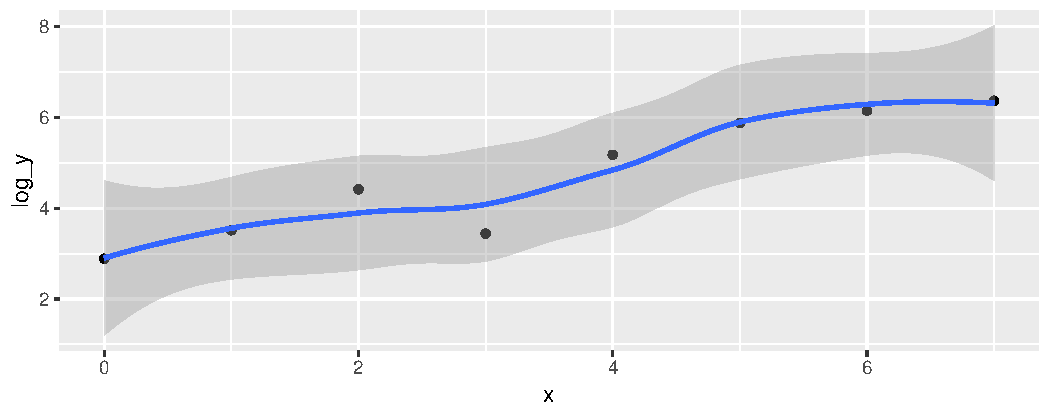
\includegraphics[width=\maxwidth]{figure/unnamed-chunk-22-1} 

\end{knitrout}
  
  
\end{frame}


\begin{frame}[fragile]{Discussion of survival curves}

  \begin{itemize}
  \item Best survival is yellow curve, stratum 2, females with
    (\texttt{ph.ecog}) score 0.
    \item Next best: dark green, stratum 4, females with score 1, and
      red, stratum 1, males score 0.
    \item Worst: purple, stratum 7, males score 3.
      \item For any given \texttt{ph.ecog} score, females have better
        predicted survival than males.
      \item For both genders, a lower score associated with better
        survival.
  \item \texttt{sex} coeff in model 3 negative, so being higher
    \texttt{sex} value (female) goes with \emph{less} hazard of dying.
  \item \texttt{ph.ecog} coeff in model 3 positive, so higher
    \texttt{ph.ecog} score goes with \emph{more} hazard of dying
  \item Two coeffs about same size, so being male rather than female
    corresponds to 1-point increase in \texttt{ph.ecog} score. Note
    how survival curves come in 3 pairs plus 2 odd.
  \end{itemize}

\end{frame}


\begin{frame}[fragile]{Martingale residuals for this model}
  
\begin{knitrout}
\definecolor{shadecolor}{rgb}{0.969, 0.969, 0.969}\color{fgcolor}\begin{kframe}
\begin{alltt}
\hlkwd{ggcoxdiagnostics}\hlstd{(lung.3)}\hlopt{+}\hlkwd{geom_smooth}\hlstd{(}\hlkwc{se}\hlstd{=F)}
\end{alltt}


{\ttfamily\noindent\itshape\color{messagecolor}{\#\# `geom\_smooth()` using method = 'loess'}}\end{kframe}
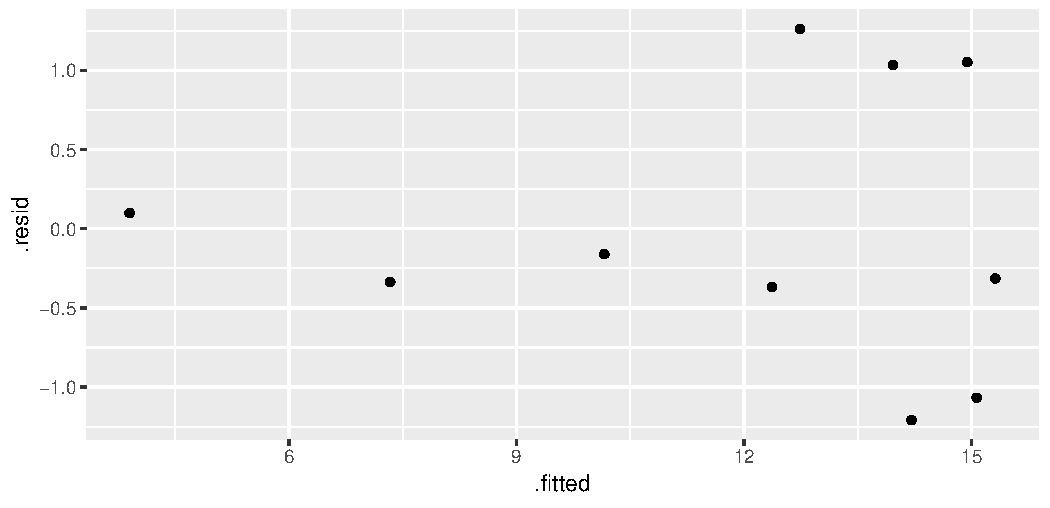
\includegraphics[width=\maxwidth]{figure/unnamed-chunk-23-1} 

\end{knitrout}

No problems here.
  
\end{frame}


\begin{frame}[fragile]{When the Cox model fails}
  \begin{itemize}
  \item Invent some data where survival is best at middling age, and
    worse at high \emph{and} low age:

\begin{knitrout}
\definecolor{shadecolor}{rgb}{0.969, 0.969, 0.969}\color{fgcolor}\begin{kframe}
\begin{alltt}
\hlstd{age}\hlkwb{=}\hlkwd{seq}\hlstd{(}\hlnum{20}\hlstd{,}\hlnum{60}\hlstd{,}\hlnum{5}\hlstd{)}
\hlstd{survtime}\hlkwb{=}\hlkwd{c}\hlstd{(}\hlnum{10}\hlstd{,}\hlnum{12}\hlstd{,}\hlnum{11}\hlstd{,}\hlnum{21}\hlstd{,}\hlnum{15}\hlstd{,}\hlnum{20}\hlstd{,}\hlnum{8}\hlstd{,}\hlnum{9}\hlstd{,}\hlnum{11}\hlstd{)}
\hlstd{stat}\hlkwb{=}\hlkwd{c}\hlstd{(}\hlnum{1}\hlstd{,}\hlnum{1}\hlstd{,}\hlnum{1}\hlstd{,}\hlnum{1}\hlstd{,}\hlnum{0}\hlstd{,}\hlnum{1}\hlstd{,}\hlnum{1}\hlstd{,}\hlnum{1}\hlstd{,}\hlnum{1}\hlstd{)}
\hlstd{d}\hlkwb{=}\hlkwd{data.frame}\hlstd{(age,survtime,stat)}
\hlstd{y}\hlkwb{=}\hlkwd{with}\hlstd{(d,}\hlkwd{Surv}\hlstd{(survtime,stat))}
\end{alltt}
\end{kframe}
\end{knitrout}

\item Small survival time 15 in middle was actually censored, so would
  have been longer if observed.
  \end{itemize}
\end{frame}

\begin{frame}[fragile]{Fit Cox model}
  
  \begin{footnotesize}
\begin{knitrout}
\definecolor{shadecolor}{rgb}{0.969, 0.969, 0.969}\color{fgcolor}\begin{kframe}
\begin{alltt}
\hlstd{y.1}\hlkwb{=}\hlkwd{coxph}\hlstd{(y}\hlopt{~}\hlstd{age,}\hlkwc{data}\hlstd{=d)}
\hlkwd{summary}\hlstd{(y.1)}
\end{alltt}
\begin{verbatim}
## Call:
## coxph(formula = y ~ age, data = d)
## 
##   n= 9, number of events= 8 
## 
##        coef exp(coef) se(coef)     z Pr(>|z|)
## age 0.01984   1.02003  0.03446 0.576    0.565
## 
##     exp(coef) exp(-coef) lower .95 upper .95
## age      1.02     0.9804    0.9534     1.091
## 
## Concordance= 0.545  (se = 0.146 )
## Rsquare= 0.036   (max possible= 0.926 )
## Likelihood ratio test= 0.33  on 1 df,   p=0.5669
## Wald test            = 0.33  on 1 df,   p=0.5649
## Score (logrank) test = 0.33  on 1 df,   p=0.563
\end{verbatim}
\end{kframe}
\end{knitrout}
    
  \end{footnotesize}
  
\end{frame}

\begin{frame}[fragile]{Martingale residuals}

\begin{knitrout}
\definecolor{shadecolor}{rgb}{0.969, 0.969, 0.969}\color{fgcolor}\begin{kframe}
\begin{alltt}
\hlkwd{ggcoxdiagnostics}\hlstd{(y.1)}\hlopt{+}\hlkwd{geom_smooth}\hlstd{(}\hlkwc{se}\hlstd{=F)}
\end{alltt}


{\ttfamily\noindent\itshape\color{messagecolor}{\#\# `geom\_smooth()` using method = 'loess'}}\end{kframe}
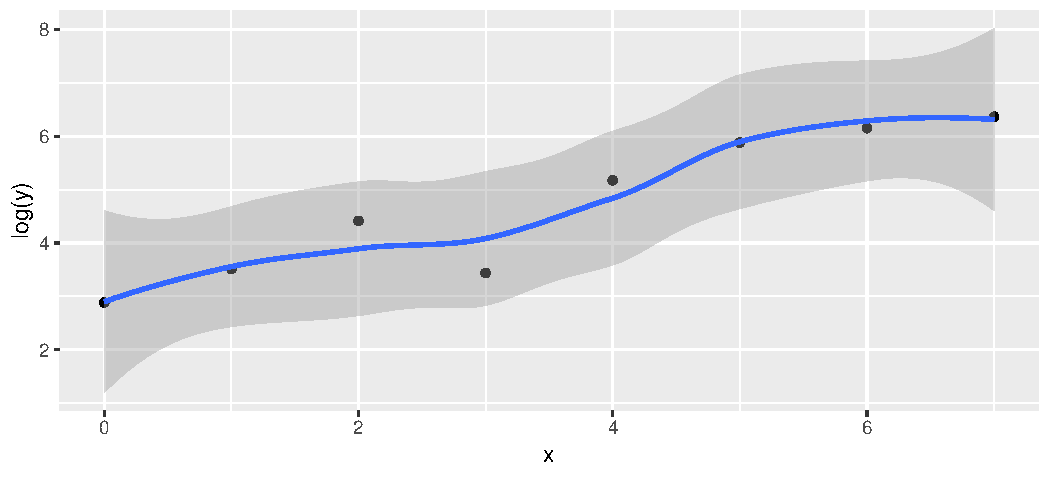
\includegraphics[width=\maxwidth]{figure/unnamed-chunk-26-1} 

\end{knitrout}

Down-and-up indicates incorrect relationship between age and
survival. Add age-squared term.
\end{frame}

\begin{frame}[fragile]{Attempt 2}
  
  \begin{footnotesize}
\begin{knitrout}
\definecolor{shadecolor}{rgb}{0.969, 0.969, 0.969}\color{fgcolor}\begin{kframe}
\begin{alltt}
\hlstd{y.2}\hlkwb{=}\hlkwd{coxph}\hlstd{(y}\hlopt{~}\hlstd{age}\hlopt{+}\hlkwd{I}\hlstd{(age}\hlopt{^}\hlnum{2}\hlstd{),}\hlkwc{data}\hlstd{=d)}
\hlkwd{summary}\hlstd{(y.2)}
\end{alltt}
\begin{verbatim}
## Call:
## coxph(formula = y ~ age + I(age^2), data = d)
## 
##   n= 9, number of events= 8 
## 
##               coef exp(coef)  se(coef)      z Pr(>|z|)  
## age      -0.380184  0.683736  0.241617 -1.573   0.1156  
## I(age^2)  0.004832  1.004844  0.002918  1.656   0.0977 .
## ---
## Signif. codes:  0 '***' 0.001 '**' 0.01 '*' 0.05 '.' 0.1 ' ' 1
## 
##          exp(coef) exp(-coef) lower .95 upper .95
## age         0.6837     1.4626    0.4258     1.098
## I(age^2)    1.0048     0.9952    0.9991     1.011
## 
## Concordance= 0.758  (se = 0.146 )
## Rsquare= 0.304   (max possible= 0.926 )
## Likelihood ratio test= 3.26  on 2 df,   p=0.1964
## Wald test            = 3.16  on 2 df,   p=0.2058
## Score (logrank) test = 3.75  on 2 df,   p=0.1536
\end{verbatim}
\end{kframe}
\end{knitrout}
  \end{footnotesize}
  
\end{frame}

\begin{frame}[fragile]{Martingale residuals this time}
  
\begin{knitrout}
\definecolor{shadecolor}{rgb}{0.969, 0.969, 0.969}\color{fgcolor}\begin{kframe}
\begin{alltt}
\hlkwd{ggcoxdiagnostics}\hlstd{(y.2)}\hlopt{+}\hlkwd{geom_smooth}\hlstd{(}\hlkwc{se}\hlstd{=F)}
\end{alltt}


{\ttfamily\noindent\itshape\color{messagecolor}{\#\# `geom\_smooth()` using method = 'loess'}}\end{kframe}
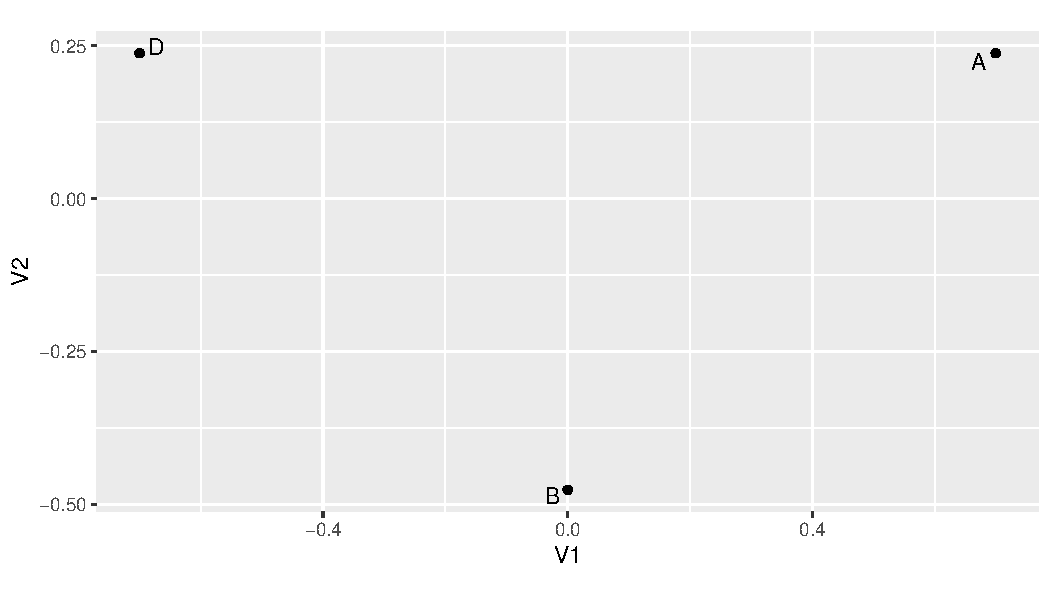
\includegraphics[width=\maxwidth]{figure/unnamed-chunk-28-1} 

\end{knitrout}

Not great, but less problematic than before.
  
\end{frame}


\section{Analysis of variance}
\frame{\sectionpage}

\begin{frame}[fragile]{Analysis of variance}

  \begin{itemize}
  \item Analysis of variance used with:
    \begin{itemize}
    \item counted/measured response
    \item categorical explanatory variable(s)
    \item that is, data divided into groups, and see if response significantly different among groups
    \item or, see whether knowing group membership helps to predict response.
    \end{itemize}
  \item Typically two stages:
    \begin{itemize}
    \item $F$-test to detect {\em any} differences among/due to groups
    \item if $F$-test significant, do {\em multiple comparisons} to see which groups significantly different from which.
    \item Need special multiple comparisons method because just doing (say) two-sample $t$-tests on each pair of groups gives too big a chance of finding ``significant'' differences by accident.
    \end{itemize}
  \end{itemize}
  
\end{frame}

\begin{frame}[fragile]{Example: Pain threshold and hair colour}
  
  \begin{itemize}
  \item Do people with different hair colour have different abilities
    to deal with pain?
  \item Men and women of various ages divided into 4 groups by hair
    colour: light and dark blond, light and dark brown.
  \item Each subject given a pain sensitivity test resulting in pain
    threshold score: higher score is higher pain tolerance.
  \item 19 subjects altogether.
  \end{itemize}

\end{frame}

\begin{frame}[fragile]{The data}
  
  In \texttt{hairpain.txt}:
  
  \begin{multicols}{2}
\begin{verbatim}
hair pain
lightblond 62
lightblond 60
lightblond 71
lightblond 55
lightblond 48
darkblond 63
darkblond 57
darkblond 52
darkblond 41
darkblond 43
lightbrown 42
lightbrown 50
lightbrown 41
lightbrown 37
darkbrown 32
darkbrown 39
darkbrown 51
darkbrown 30
darkbrown 35
\end{verbatim}
  \end{multicols}
  
\end{frame}

\begin{frame}[fragile]{Summarizing the groups}
  
  \begin{itemize}
    

  \item Read in data:
    
\begin{knitrout}
\definecolor{shadecolor}{rgb}{0.969, 0.969, 0.969}\color{fgcolor}\begin{kframe}
\begin{alltt}
\hlstd{hairpain}\hlkwb{=}\hlkwd{read.table}\hlstd{(}\hlstr{"hairpain.txt"}\hlstd{,}\hlkwc{header}\hlstd{=T)}
\end{alltt}
\end{kframe}
\end{knitrout}

\item then \texttt{aggregate}:
  
\begin{knitrout}
\definecolor{shadecolor}{rgb}{0.969, 0.969, 0.969}\color{fgcolor}\begin{kframe}
\begin{alltt}
\hlkwd{aggregate}\hlstd{(pain}\hlopt{~}\hlstd{hair,hairpain,mean)}
\end{alltt}
\begin{verbatim}
##         hair pain
## 1  darkblond 51.2
## 2  darkbrown 37.4
## 3 lightblond 59.2
## 4 lightbrown 42.5
\end{verbatim}
\end{kframe}
\end{knitrout}

\item Brown-haired people seem to have lower pain tolerance. 
  \end{itemize}
  
\end{frame}

\begin{frame}[fragile]{Or, better summary}
  
Use \texttt{dplyr}:

\begin{knitrout}
\definecolor{shadecolor}{rgb}{0.969, 0.969, 0.969}\color{fgcolor}\begin{kframe}
\begin{alltt}
\hlkwd{suppressMessages}\hlstd{(}\hlkwd{library}\hlstd{(dplyr))}
\hlstd{hairpain} \hlopt \hlkwd{group_by}\hlstd{(hair)} \hlopt
  \hlkwd{summarize}\hlstd{(} \hlkwc{n}\hlstd{=}\hlkwd{n}\hlstd{(),}
             \hlkwc{xbar}\hlstd{=}\hlkwd{mean}\hlstd{(pain),}
             \hlkwc{s}\hlstd{=}\hlkwd{sd}\hlstd{(pain))}
\end{alltt}
\begin{verbatim}
## # A tibble: 4 × 4
##         hair     n  xbar        s
##       <fctr> <int> <dbl>    <dbl>
## 1  darkblond     5  51.2 9.284396
## 2  darkbrown     5  37.4 8.324662
## 3 lightblond     5  59.2 8.526429
## 4 lightbrown     4  42.5 5.446712
\end{verbatim}
\end{kframe}
\end{knitrout}
  
\end{frame}

\begin{frame}[fragile]{Boxplot}
  
\begin{knitrout}
\definecolor{shadecolor}{rgb}{0.969, 0.969, 0.969}\color{fgcolor}\begin{kframe}
\begin{alltt}
\hlkwd{ggplot}\hlstd{(hairpain,}\hlkwd{aes}\hlstd{(}\hlkwc{x}\hlstd{=hair,}\hlkwc{y}\hlstd{=pain))}\hlopt{+}\hlkwd{geom_boxplot}\hlstd{()}
\end{alltt}
\end{kframe}
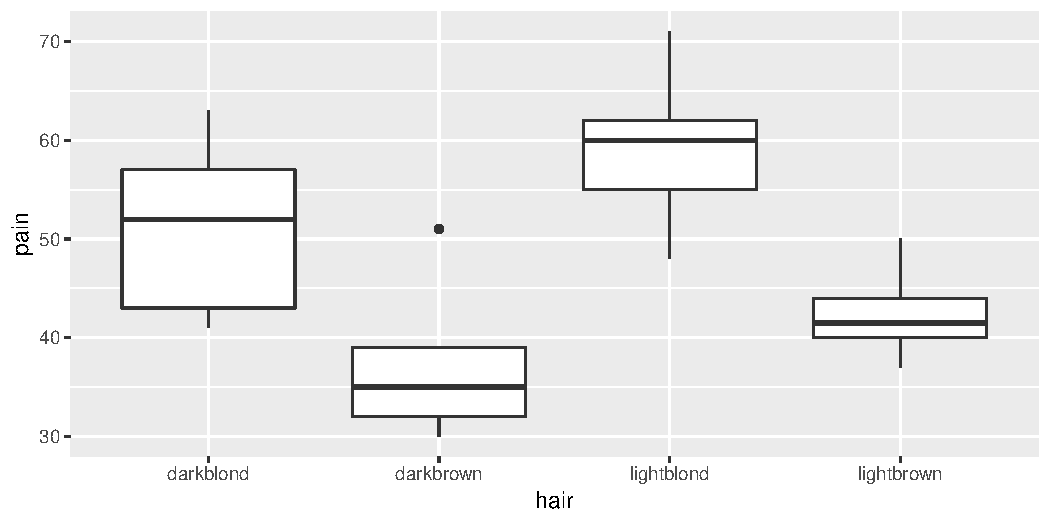
\includegraphics[width=\maxwidth]{figure/tartuffo-1} 

\end{knitrout}
  
\end{frame}

\begin{frame}[fragile]{Assumptions}
  
  \begin{itemize}
  \item Data should be:
    \begin{itemize}
    \item normally distributed within each group
    \item same spread for each group
    \end{itemize}

  \item \texttt{darkbrown} group has upper outlier (suggests not normal)
  \item \texttt{darkblond} group has smaller IQR than other groups.
  \item But, groups \emph{small}.
  \item Shrug shoulders and continue.
  \end{itemize}
  
\end{frame}

\begin{frame}[fragile]{Testing equality of SDs}
  
  
  \begin{itemize}
  \item   via \textbf{Levene's test}:
    {\small
\begin{knitrout}
\definecolor{shadecolor}{rgb}{0.969, 0.969, 0.969}\color{fgcolor}\begin{kframe}
\begin{alltt}
\hlstd{car}\hlopt{::}\hlkwd{leveneTest}\hlstd{(pain}\hlopt{~}\hlstd{hair,}\hlkwc{data}\hlstd{=hairpain)}
\end{alltt}
\begin{verbatim}
## Levene's Test for Homogeneity of Variance (center = median)
##       Df F value Pr(>F)
## group  3  0.3927   0.76
##       15
\end{verbatim}
\end{kframe}
\end{knitrout}
 }
\item No evidence (at all) of difference among group SDs.
\item Possibly because groups \emph{small}.
  \end{itemize}
  
\end{frame}

\begin{frame}[fragile]{Analysis of variance}
\begin{knitrout}
\definecolor{shadecolor}{rgb}{0.969, 0.969, 0.969}\color{fgcolor}\begin{kframe}
\begin{alltt}
\hlstd{hairpain.1}\hlkwb{=}\hlkwd{aov}\hlstd{(pain}\hlopt{~}\hlstd{hair,}\hlkwc{data}\hlstd{=hairpain)}
\hlkwd{summary}\hlstd{(hairpain.1)}
\end{alltt}
\begin{verbatim}
##             Df Sum Sq Mean Sq F value  Pr(>F)   
## hair         3   1361   453.6   6.791 0.00411 **
## Residuals   15   1002    66.8                   
## ---
## Signif. codes:  0 '***' 0.001 '**' 0.01 '*' 0.05 '.' 0.1 ' ' 1
\end{verbatim}
\end{kframe}
\end{knitrout}

\begin{itemize}
\item P-value small: the mean pain tolerances for the four groups are
  \emph{not} all the same.
\item Which groups differ from which, and how?
\end{itemize}
\end{frame}



\begin{frame}[fragile]{Multiple comparisons}

  \begin{itemize}
  \item Which groups differ from which? Multiple
    comparisons method. Lots.
  \item Problem: by comparing all the groups with each other, doing
    many tests, have large chance to (possibly incorrectly) reject
    $H_0:$ groups have equal means.
  \item 4 groups: 6 comparisons (1 vs 2, 1 vs 3, \ldots, 3 vs 4). 5 groups: 10
    comparisons. Thus 6 (or 10) chances to make mistake.
\item Get ``familywise error rate'' of 0.05 (whatever), no
matter how many comparisons you’re doing.
\item My favourite: Tukey, or ``honestly
  significant differences'': how far apart might largest, smallest
  group means be (if actually no differences). Group means more
  different: significantly different.
  \end{itemize}
\end{frame}

\begin{frame}[fragile]{Tukey}

  \begin{itemize}
  \item \texttt{TukeyHSD:}

{\footnotesize
 
\begin{knitrout}
\definecolor{shadecolor}{rgb}{0.969, 0.969, 0.969}\color{fgcolor}\begin{kframe}
\begin{alltt}
\hlkwd{TukeyHSD}\hlstd{(hairpain.1)}
\end{alltt}
\begin{verbatim}
##   Tukey multiple comparisons of means
##     95% family-wise confidence level
## 
## Fit: aov(formula = pain ~ hair, data = hairpain)
## 
## $hair
##                        diff        lwr        upr     p adj
## darkbrown-darkblond   -13.8 -28.696741  1.0967407 0.0740679
## lightblond-darkblond    8.0  -6.896741 22.8967407 0.4355768
## lightbrown-darkblond   -8.7 -24.500380  7.1003795 0.4147283
## lightblond-darkbrown   21.8   6.903259 36.6967407 0.0037079
## lightbrown-darkbrown    5.1 -10.700380 20.9003795 0.7893211
## lightbrown-lightblond -16.7 -32.500380 -0.8996205 0.0366467
\end{verbatim}
\end{kframe}
\end{knitrout}
}



  \end{itemize}



\end{frame}

\begin{frame}[fragile]{The old-fashioned way}
  
  \begin{itemize}
  \item List group means in order
  \item Draw lines connecting groups that are \emph{not} significantly
    different:
    
\begin{verbatim}
darkbrown lightbrown  darkblond lightblond
   37.4      42.5       51.2       59.2
   -------------------------
                        ---------------
\end{verbatim}

  \item \texttt{lightblond} significantly higher than everything
    except \texttt{darkblond} (at $\alpha=0.05$).
  \item \texttt{darkblond} in middle ground: not significantly less
    than \texttt{lightblond}, not significantly greater than
    \texttt{darkbrown} and \texttt{lightbrown}.
  \item More data might resolve this.
  \item Looks as if blond-haired people do have higher pain tolerance,
    but not completely clear.
  \end{itemize}
  
\end{frame}


\begin{frame}[fragile]{Some other multiple-comparison methods}

  \begin{itemize}
  \item P-values 0.005, 0.015, 0.03, 0.06 (4 tests all done at once)
Use $\alpha=0.05$.

\item Bonferroni: 
  \begin{itemize}
  \item 
Multiply all P-values by 4 (4 tests).
\item 
Reject only 1st null.
  \end{itemize}

\item Holm: 
  \begin{itemize}
  \item 
Times smallest P-value by 4: $0.005*4=0.020<0.05$, reject.
\item 
Times next smallest by 3: $0.015*3=0.045<0.05$, reject.
\item Times next smallest by 2: $0.03*2=0.06>0.05$, do not reject. Stop.
  \end{itemize}

\item False discovery rate:
  \begin{itemize}
  \item 
Times smallest P-value by 4: $0.005*4=0.02<0.05$: reject.
\item Times second smallest by $4/2$: $0.015*4/2=0.03<0.05$, reject.
\item Times third smallest by $4/3$: $0.03*4/3=0.04<0.05$, reject.
\item Times fourth smallest by $4/4$: 0.06*4/4=0.06>0.05, do not reject. Stop.
  \end{itemize}
  \end{itemize}
  
\end{frame}

\begin{frame}[fragile]{\texttt{pairwise.t.test}}

  \begin{multicols}{2}
{\tiny
\begin{knitrout}
\definecolor{shadecolor}{rgb}{0.969, 0.969, 0.969}\color{fgcolor}\begin{kframe}
\begin{alltt}
\hlkwd{attach}\hlstd{(hairpain)}
\hlkwd{pairwise.t.test}\hlstd{(pain,hair,}\hlkwc{p.adj}\hlstd{=}\hlstr{"none"}\hlstd{)}
\end{alltt}
\begin{verbatim}
## 
## 	Pairwise comparisons using t tests with pooled SD 
## 
## data:  pain and hair 
## 
##            darkblond darkbrown lightblond
## darkbrown  0.01748   -         -         
## lightblond 0.14251   0.00075   -         
## lightbrown 0.13337   0.36695   0.00817   
## 
## P value adjustment method: none
\end{verbatim}
\begin{alltt}
\hlkwd{pairwise.t.test}\hlstd{(pain,hair,}\hlkwc{p.adj}\hlstd{=}\hlstr{"holm"}\hlstd{)}
\end{alltt}
\begin{verbatim}
## 
## 	Pairwise comparisons using t tests with pooled SD 
## 
## data:  pain and hair 
## 
##            darkblond darkbrown lightblond
## darkbrown  0.0699    -         -         
## lightblond 0.4001    0.0045    -         
## lightbrown 0.4001    0.4001    0.0408    
## 
## P value adjustment method: holm
\end{verbatim}
\end{kframe}
\end{knitrout}

\begin{knitrout}
\definecolor{shadecolor}{rgb}{0.969, 0.969, 0.969}\color{fgcolor}\begin{kframe}
\begin{alltt}
\hlkwd{pairwise.t.test}\hlstd{(pain,hair,}\hlkwc{p.adj}\hlstd{=}\hlstr{"fdr"}\hlstd{)}
\end{alltt}
\begin{verbatim}
## 
## 	Pairwise comparisons using t tests with pooled SD 
## 
## data:  pain and hair 
## 
##            darkblond darkbrown lightblond
## darkbrown  0.0350    -         -         
## lightblond 0.1710    0.0045    -         
## lightbrown 0.1710    0.3670    0.0245    
## 
## P value adjustment method: fdr
\end{verbatim}
\begin{alltt}
\hlkwd{pairwise.t.test}\hlstd{(pain,hair,}\hlkwc{p.adj}\hlstd{=}\hlstr{"bon"}\hlstd{)}
\end{alltt}
\begin{verbatim}
## 
## 	Pairwise comparisons using t tests with pooled SD 
## 
## data:  pain and hair 
## 
##            darkblond darkbrown lightblond
## darkbrown  0.1049    -         -         
## lightblond 0.8550    0.0045    -         
## lightbrown 0.8002    1.0000    0.0490    
## 
## P value adjustment method: bonferroni
\end{verbatim}
\end{kframe}
\end{knitrout}
}
    
  \end{multicols}
  
\end{frame}

\begin{frame}[fragile]{Comments}
  
  \begin{itemize}
  \item P-values all adjusted upwards from ``none''.
  \item Required because 6 tests at once.
  \item Highest P-values for Bonferroni: most ``conservative''.
  \item Prefer Tukey or FDR or Holm.
  \item Tukey only applies to ANOVA, not to other cases of multiple
    testing. 
  \end{itemize}
  
\end{frame}

\begin{frame}[fragile]{Rats and vitamin B}
  
  \begin{itemize}
  \item What is the effect of dietary vitamin B on the kidney?
  \item A number of rats were randomized to receive either a
    B-supplemented diet or a regular diet.
  \item Desired to control for initial size of rats, so classified
    into size classes \texttt{lean} and \texttt{obese}.
  \item After 20 weeks, rats' kidneys weighed.
  \item Variables:
    \begin{itemize}
    \item Response: \texttt{kidneyweight} (grams).
    \item Explanatory: \texttt{diet}, \texttt{ratsize}.
    \end{itemize}
  \item Read in data:
    
\begin{knitrout}
\definecolor{shadecolor}{rgb}{0.969, 0.969, 0.969}\color{fgcolor}\begin{kframe}
\begin{alltt}
\hlstd{vitaminb}\hlkwb{=}\hlkwd{read.table}\hlstd{(}\hlstr{"vitaminb.txt"}\hlstd{,}\hlkwc{header}\hlstd{=T)}
\end{alltt}
\end{kframe}
\end{knitrout}
  \end{itemize}
  
\end{frame}

\begin{frame}[fragile]{What's going on?}
  
  \begin{itemize}
  \item Calculate group means:
    
\begin{knitrout}
\definecolor{shadecolor}{rgb}{0.969, 0.969, 0.969}\color{fgcolor}\begin{kframe}
\begin{alltt}
\hlstd{vitaminb} \hlopt \hlkwd{group_by}\hlstd{(ratsize,diet)} \hlopt
  \hlkwd{summarize}\hlstd{(}\hlkwc{mean}\hlstd{=}\hlkwd{mean}\hlstd{(kidneyweight))} \hlkwb{->} \hlstd{summary}
\hlstd{summary}
\end{alltt}
\begin{verbatim}
## Source: local data frame [4 x 3]
## Groups: ratsize [?]
## 
##   ratsize     diet     mean
##    <fctr>   <fctr>    <dbl>
## 1    lean  regular 1.641429
## 2    lean vitaminb 1.527143
## 3   obese  regular 2.642857
## 4   obese vitaminb 2.672857
\end{verbatim}
\end{kframe}
\end{knitrout}
\item Rat size: a large and consistent effect.
\item Diet: no effect (compare same rat size, different
  diet).
\item Effect of rat size \emph{same} for each diet: no interaction.
  \end{itemize}

\end{frame}

\begin{frame}[fragile]{ANOVA with interaction}
  
\begin{knitrout}
\definecolor{shadecolor}{rgb}{0.969, 0.969, 0.969}\color{fgcolor}\begin{kframe}
\begin{alltt}
\hlstd{vitaminb.1}\hlkwb{=}\hlkwd{aov}\hlstd{(kidneyweight}\hlopt{~}\hlstd{ratsize}\hlopt{*}\hlstd{diet,}\hlkwc{data}\hlstd{=vitaminb)}
\hlkwd{summary}\hlstd{(vitaminb.1)}
\end{alltt}
\begin{verbatim}
##              Df Sum Sq Mean Sq F value   Pr(>F)    
## ratsize       1  8.068   8.068 141.179 1.53e-11 ***
## diet          1  0.012   0.012   0.218    0.645    
## ratsize:diet  1  0.036   0.036   0.638    0.432    
## Residuals    24  1.372   0.057                     
## ---
## Signif. codes:  0 '***' 0.001 '**' 0.01 '*' 0.05 '.' 0.1 ' ' 1
\end{verbatim}
\end{kframe}
\end{knitrout}

Significance/nonsignificance as we expected. Note no significant
interaction (can be removed). 
  
\end{frame}

\begin{frame}[fragile]{Interaction plot}
  
  \begin{itemize}
  \item Plot mean of response variable against one of the explanatory, using
    other one as groups. Start from summary:
    
\begin{knitrout}
\definecolor{shadecolor}{rgb}{0.969, 0.969, 0.969}\color{fgcolor}\begin{kframe}
\begin{alltt}
\hlstd{g}\hlkwb{=}\hlkwd{ggplot}\hlstd{(summary,}\hlkwd{aes}\hlstd{(}\hlkwc{x}\hlstd{=ratsize,}\hlkwc{y}\hlstd{=mean,}
     \hlkwc{colour}\hlstd{=diet,}\hlkwc{group}\hlstd{=diet))}\hlopt{+}
  \hlkwd{geom_point}\hlstd{()}\hlopt{+}\hlkwd{geom_line}\hlstd{()}
\end{alltt}
\end{kframe}
\end{knitrout}

\item For this, have to give \emph{both} \texttt{group} and \texttt{colour}.
  \end{itemize}
  
\end{frame}

\begin{frame}[fragile]{The interaction plot}
\begin{knitrout}
\definecolor{shadecolor}{rgb}{0.969, 0.969, 0.969}\color{fgcolor}\begin{kframe}
\begin{alltt}
\hlstd{g}
\end{alltt}
\end{kframe}
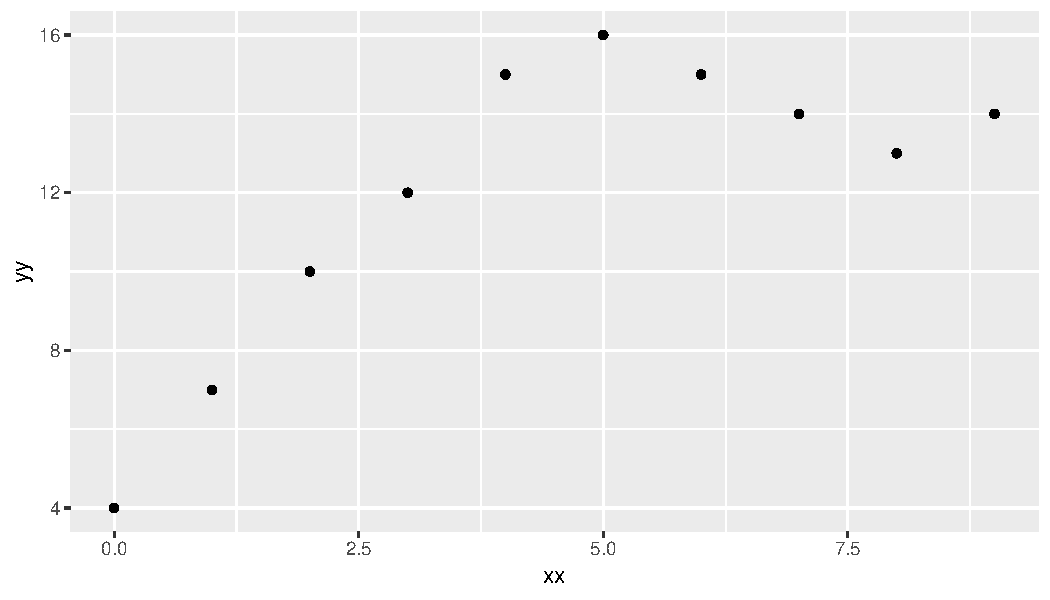
\includegraphics[width=\maxwidth]{figure/unnamed-chunk-14-1} 

\end{knitrout}

Lines basically parallel, indicating no interaction.
\end{frame}

\begin{frame}[fragile]{Take out interaction}
  
\begin{knitrout}
\definecolor{shadecolor}{rgb}{0.969, 0.969, 0.969}\color{fgcolor}\begin{kframe}
\begin{alltt}
\hlstd{vitaminb.2}\hlkwb{=}\hlkwd{aov}\hlstd{(kidneyweight}\hlopt{~}\hlstd{ratsize}\hlopt{+}\hlstd{diet,}\hlkwc{data}\hlstd{=vitaminb)}
\hlkwd{summary}\hlstd{(vitaminb.2)}
\end{alltt}
\begin{verbatim}
##             Df Sum Sq Mean Sq F value   Pr(>F)    
## ratsize      1  8.068   8.068 143.256 7.59e-12 ***
## diet         1  0.012   0.012   0.221    0.643    
## Residuals   25  1.408   0.056                     
## ---
## Signif. codes:  0 '***' 0.001 '**' 0.01 '*' 0.05 '.' 0.1 ' ' 1
\end{verbatim}
\end{kframe}
\end{knitrout}

\begin{itemize}
\item No Tukey for \texttt{diet}: not significant.
\item No Tukey for \texttt{ratsize}: only two sizes, and already know
  that obese rats have larger kidneys than lean ones.
\item Bottom line: diet has no effect on kidney size once you control
  for size of rat.
\end{itemize}
  
\end{frame}



\begin{frame}[fragile]{The auto noise data}
  
  In 1973, the President of Texaco cited an automobile filter
  developed by Associated Octel Company as effective in reducing
  pollution. However, questions had been raised about the effects of
  filter silencing. He referred to the data included in the report
  (and below) as evidence
  that the silencing properties of the Octel filter were at least
  equal to those of standard silencers. 
 
\begin{knitrout}
\definecolor{shadecolor}{rgb}{0.969, 0.969, 0.969}\color{fgcolor}\begin{kframe}
\begin{alltt}
\hlstd{autonoise}\hlkwb{=}\hlkwd{read.table}\hlstd{(}\hlstr{"autonoise.txt"}\hlstd{,}\hlkwc{header}\hlstd{=T)}
\hlkwd{str}\hlstd{(autonoise)}
\end{alltt}
\begin{verbatim}
## 'data.frame':	36 obs. of  4 variables:
##  $ noise: int  840 770 820 775 825 840 845 825 815 845 ...
##  $ size : Factor w/ 3 levels "L","M","S": 2 1 2 1 2 2 2 2 2 2 ...
##  $ type : Factor w/ 2 levels "Octel","Std": 2 1 1 1 1 2 2 1 1 2 ...
##  $ side : Factor w/ 2 levels "L","R": 2 1 2 2 1 2 1 1 1 2 ...
\end{verbatim}
\end{kframe}
\end{knitrout}
  
\end{frame}

\begin{frame}[fragile]{Making boxplot}
  
  \begin{itemize}
  \item Make a boxplot, but have combinations of filter type and
    engine size.
  \item Make a column that is the two of them glued together, and then
    use as $x$ for boxplot:
    
\begin{knitrout}
\definecolor{shadecolor}{rgb}{0.969, 0.969, 0.969}\color{fgcolor}\begin{kframe}
\begin{alltt}
\hlstd{autonoise} \hlopt \hlkwd{unite}\hlstd{(sizetype,}\hlkwd{c}\hlstd{(size,type))} \hlopt \hlkwd{head}\hlstd{()}
\end{alltt}
\begin{verbatim}
##   noise sizetype side
## 1   840    M_Std    R
## 2   770  L_Octel    L
## 3   820  M_Octel    R
## 4   775  L_Octel    R
## 5   825  M_Octel    L
## 6   840    M_Std    R
\end{verbatim}
\end{kframe}
\end{knitrout}

\item Pipe also plays with \texttt{ggplot}, thus:
  
\begin{knitrout}
\definecolor{shadecolor}{rgb}{0.969, 0.969, 0.969}\color{fgcolor}\begin{kframe}
\begin{alltt}
\hlstd{autonoise} \hlopt \hlkwd{unite}\hlstd{(sizetype,}\hlkwd{c}\hlstd{(size,type))} \hlopt
  \hlkwd{ggplot}\hlstd{(}\hlkwd{aes}\hlstd{(}\hlkwc{x}\hlstd{=sizetype,}\hlkwc{y}\hlstd{=noise))}\hlopt{+}\hlkwd{geom_boxplot}\hlstd{()} \hlkwb{->} \hlstd{g}
\end{alltt}
\end{kframe}
\end{knitrout}
  \end{itemize}
  
  
\end{frame}

\begin{frame}[fragile]{The boxplot}
\begin{knitrout}
\definecolor{shadecolor}{rgb}{0.969, 0.969, 0.969}\color{fgcolor}\begin{kframe}
\begin{alltt}
\hlstd{g}
\end{alltt}
\end{kframe}
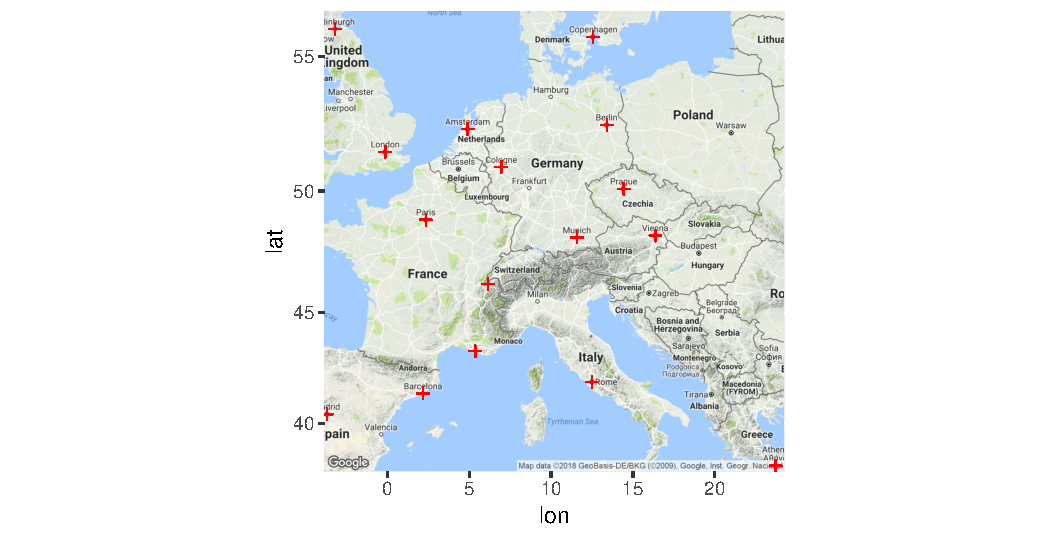
\includegraphics[width=\maxwidth]{figure/unnamed-chunk-19-1} 

\end{knitrout}

Difference in engine noise between Octel and standard is larger for
medium engine size than for large or small.
\end{frame}


\begin{frame}[fragile]{ANOVA}
  
\begin{knitrout}
\definecolor{shadecolor}{rgb}{0.969, 0.969, 0.969}\color{fgcolor}\begin{kframe}
\begin{alltt}
\hlstd{autonoise.1}\hlkwb{=}\hlkwd{aov}\hlstd{(noise}\hlopt{~}\hlstd{size}\hlopt{*}\hlstd{type,}\hlkwc{data}\hlstd{=autonoise)}
\hlkwd{summary}\hlstd{(autonoise.1)}
\end{alltt}
\begin{verbatim}
##             Df Sum Sq Mean Sq F value   Pr(>F)    
## size         2  26051   13026 199.119  < 2e-16 ***
## type         1   1056    1056  16.146 0.000363 ***
## size:type    2    804     402   6.146 0.005792 ** 
## Residuals   30   1962      65                     
## ---
## Signif. codes:  0 '***' 0.001 '**' 0.01 '*' 0.05 '.' 0.1 ' ' 1
\end{verbatim}
\end{kframe}
\end{knitrout}

\begin{itemize}
\item The interaction is significant, as we suspected from the boxplots.
\item The within-group spreads don't look very equal, but only based
  on 6 obs each.
\end{itemize}
  
\end{frame}

\begin{frame}[fragile]{Tukey: ouch!}
  
{\footnotesize
\begin{knitrout}
\definecolor{shadecolor}{rgb}{0.969, 0.969, 0.969}\color{fgcolor}\begin{kframe}
\begin{alltt}
\hlstd{autonoise.2}\hlkwb{=}\hlkwd{TukeyHSD}\hlstd{(autonoise.1)}
\hlstd{autonoise.2}\hlopt{$}\hlstd{`size:type`}
\end{alltt}
\begin{verbatim}
##                        diff        lwr        upr        p adj
## M:Octel-L:Octel  51.6666667  37.463511  65.869823 6.033496e-11
## S:Octel-L:Octel  52.5000000  38.296844  66.703156 4.089762e-11
## L:Std-L:Octel     5.0000000  -9.203156  19.203156 8.890358e-01
## M:Std-L:Octel    75.8333333  61.630177  90.036489 4.962697e-14
## S:Std-L:Octel    55.8333333  41.630177  70.036489 9.002910e-12
## S:Octel-M:Octel   0.8333333 -13.369823  15.036489 9.999720e-01
## L:Std-M:Octel   -46.6666667 -60.869823 -32.463511 6.766649e-10
## M:Std-M:Octel    24.1666667   9.963511  38.369823 1.908995e-04
## S:Std-M:Octel     4.1666667 -10.036489  18.369823 9.454142e-01
## L:Std-S:Octel   -47.5000000 -61.703156 -33.296844 4.477636e-10
## M:Std-S:Octel    23.3333333   9.130177  37.536489 3.129974e-04
## S:Std-S:Octel     3.3333333 -10.869823  17.536489 9.787622e-01
## M:Std-L:Std      70.8333333  56.630177  85.036489 6.583623e-14
## S:Std-L:Std      50.8333333  36.630177  65.036489 8.937329e-11
## S:Std-M:Std     -20.0000000 -34.203156  -5.796844 2.203265e-03
\end{verbatim}
\end{kframe}
\end{knitrout}
}
  
\end{frame}

\begin{frame}[fragile]{Interaction plot}
  
  \begin{itemize}
  \item This time, don't have summary of mean noise for each size-type
    combination. 
  \item One way is to compute summaries (means) first, and feed into
    \texttt{ggplot} as in vitamin B example.
  \item Or, have \texttt{ggplot} compute them for us, thus:
    
\begin{knitrout}
\definecolor{shadecolor}{rgb}{0.969, 0.969, 0.969}\color{fgcolor}\begin{kframe}
\begin{alltt}
\hlstd{g}\hlkwb{=}\hlkwd{ggplot}\hlstd{(autonoise,}\hlkwd{aes}\hlstd{(}\hlkwc{x}\hlstd{=size,}\hlkwc{y}\hlstd{=noise,}
    \hlkwc{colour}\hlstd{=type,}\hlkwc{group}\hlstd{=type))}\hlopt{+}
  \hlkwd{stat_summary}\hlstd{(}\hlkwc{fun.y}\hlstd{=mean,}\hlkwc{geom}\hlstd{=}\hlstr{"point"}\hlstd{)}\hlopt{+}
  \hlkwd{stat_summary}\hlstd{(}\hlkwc{fun.y}\hlstd{=mean,}\hlkwc{geom}\hlstd{=}\hlstr{"line"}\hlstd{)}
\end{alltt}
\end{kframe}
\end{knitrout}
  \end{itemize}
  
\end{frame}

\begin{frame}[fragile]{Interaction plot}
  
\begin{knitrout}
\definecolor{shadecolor}{rgb}{0.969, 0.969, 0.969}\color{fgcolor}\begin{kframe}
\begin{alltt}
\hlstd{g}
\end{alltt}
\end{kframe}
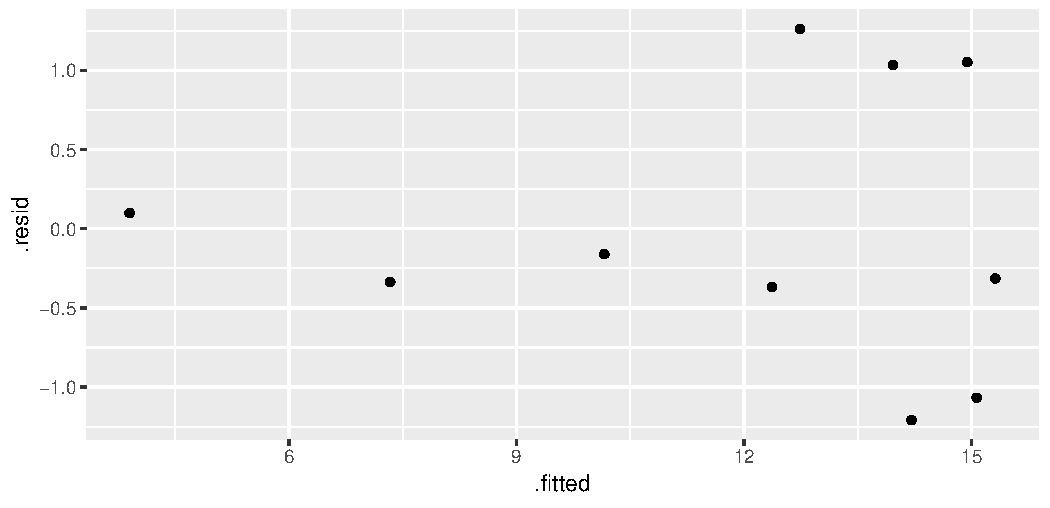
\includegraphics[width=\maxwidth]{figure/unnamed-chunk-23-1} 

\end{knitrout}

The lines are definitely \emph{not} parallel, showing that the effect
of \texttt{type} is different for medium-sized engines than for others.
  
\end{frame}

\begin{frame}[fragile]{If you don't like that\ldots}
  
  \ldots then compute the means first, in a pipe:

  \begin{small}
\begin{knitrout}
\definecolor{shadecolor}{rgb}{0.969, 0.969, 0.969}\color{fgcolor}\begin{kframe}
\begin{alltt}
\hlstd{autonoise} \hlopt \hlkwd{group_by}\hlstd{(size,type)} \hlopt
  \hlkwd{summarize}\hlstd{(}\hlkwc{mean_noise}\hlstd{=}\hlkwd{mean}\hlstd{(noise))} \hlopt
  \hlkwd{ggplot}\hlstd{(}\hlkwd{aes}\hlstd{(}\hlkwc{x}\hlstd{=size,}\hlkwc{y}\hlstd{=mean_noise,}\hlkwc{group}\hlstd{=type,}\hlkwc{colour}\hlstd{=type))}\hlopt{+}
    \hlkwd{geom_point}\hlstd{()}\hlopt{+}\hlkwd{geom_line}\hlstd{()}
\end{alltt}
\end{kframe}
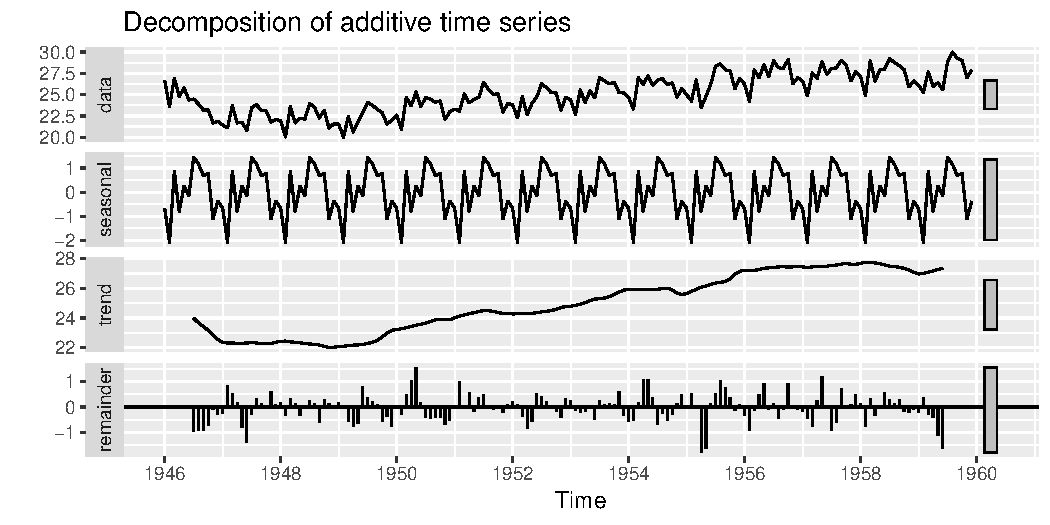
\includegraphics[width=\maxwidth]{figure/unnamed-chunk-24-1} 

\end{knitrout}
    
  \end{small}
  
\end{frame}


\begin{frame}[fragile]{Simple effects for auto noise example}
  \begin{itemize}
  \item In auto noise example, weren't interested in all comparisons
    between car size and filter type combinations.
  \item Wanted to demonstrate (lack of) difference between filter types
    \emph{for each car type}. 

  \item These are called \textbf{simple effects} of one variable
    (filter type)
    conditional on other variable (car type).

  \item To do this, pull out just the data for small cars, compare
    noise for the two filter types. Then repeat for medium and large
    cars. (Three one-way ANOVAs.)

  \end{itemize}
\end{frame}

\begin{frame}[fragile]{Do it using \texttt{dplyr} tools}
  
  \begin{itemize}
  \item Small cars:
\begin{knitrout}
\definecolor{shadecolor}{rgb}{0.969, 0.969, 0.969}\color{fgcolor}\begin{kframe}
\begin{alltt}
\hlstd{autonoise} \hlopt \hlkwd{filter}\hlstd{(size}\hlopt{==}\hlstr{"S"}\hlstd{)} \hlopt
  \hlkwd{aov}\hlstd{(noise}\hlopt{~}\hlstd{type,}\hlkwc{data}\hlstd{=.)} \hlopt \hlkwd{summary}\hlstd{()}
\end{alltt}
\begin{verbatim}
##             Df Sum Sq Mean Sq F value Pr(>F)
## type         1   33.3   33.33   0.548  0.476
## Residuals   10  608.3   60.83
\end{verbatim}
\end{kframe}
\end{knitrout}

\item No filter difference for small cars.
  

\item For Medium, change \texttt{S} to \texttt{M} and repeat.
  \end{itemize}
  
\end{frame}

\begin{frame}[fragile]{Simple effect of filter type for medium cars}
  
  {\small
\begin{knitrout}
\definecolor{shadecolor}{rgb}{0.969, 0.969, 0.969}\color{fgcolor}\begin{kframe}
\begin{alltt}
\hlstd{autonoise} \hlopt \hlkwd{filter}\hlstd{(size}\hlopt{==}\hlstr{"M"}\hlstd{)} \hlopt
  \hlkwd{aov}\hlstd{(noise}\hlopt{~}\hlstd{type,}\hlkwc{data}\hlstd{=.)} \hlopt \hlkwd{summary}\hlstd{()}
\end{alltt}
\begin{verbatim}
##             Df Sum Sq Mean Sq F value   Pr(>F)    
## type         1 1752.1  1752.1   68.93 8.49e-06 ***
## Residuals   10  254.2    25.4                     
## ---
## Signif. codes:  0 '***' 0.001 '**' 0.01 '*' 0.05 '.' 0.1 ' ' 1
\end{verbatim}
\end{kframe}
\end{knitrout}
}

\begin{itemize}
\item There \emph{is} an effect of filter type for medium cars. Look
  at means to investigate:
 
  {\footnotesize
\begin{knitrout}
\definecolor{shadecolor}{rgb}{0.969, 0.969, 0.969}\color{fgcolor}\begin{kframe}
\begin{alltt}
\hlstd{autonoise} \hlopt \hlkwd{filter}\hlstd{(size}\hlopt{==}\hlstr{"M"}\hlstd{)} \hlopt
  \hlkwd{group_by}\hlstd{(type)} \hlopt \hlkwd{summarize}\hlstd{(}\hlkwc{m}\hlstd{=}\hlkwd{mean}\hlstd{(noise))}
\end{alltt}
\begin{verbatim}
## # A tibble: 2 × 2
##     type        m
##   <fctr>    <dbl>
## 1  Octel 821.6667
## 2    Std 845.8333
\end{verbatim}
\end{kframe}
\end{knitrout}
}


  
\end{itemize}

\end{frame}


\begin{frame}[fragile]{Medium and large cars}
  
  \begin{itemize}
\item Octel filters produce \emph{less} noise for medium cars.
\item Large cars:
\begin{knitrout}
\definecolor{shadecolor}{rgb}{0.969, 0.969, 0.969}\color{fgcolor}\begin{kframe}
\begin{alltt}
\hlstd{autonoise} \hlopt \hlkwd{filter}\hlstd{(size}\hlopt{==}\hlstr{"L"}\hlstd{)} \hlopt
  \hlkwd{aov}\hlstd{(noise}\hlopt{~}\hlstd{type,}\hlkwc{data}\hlstd{=.)} \hlopt \hlkwd{summary}\hlstd{()}
\end{alltt}
\begin{verbatim}
##             Df Sum Sq Mean Sq F value Pr(>F)
## type         1     75      75   0.682  0.428
## Residuals   10   1100     110
\end{verbatim}
\end{kframe}
\end{knitrout}

\item No significant difference again.

  \end{itemize}


\end{frame}

\begin{frame}[fragile]{Simultaneous tests}
  
  \begin{itemize}
  \item When testing simple effects, doing several tests at once. (In
    this case, 3.)
  \item Have to adjust P-values for this. Eg.\ Holm:
\begin{knitrout}
\definecolor{shadecolor}{rgb}{0.969, 0.969, 0.969}\color{fgcolor}\begin{kframe}
\begin{alltt}
\hlstd{p.values}\hlkwb{=}\hlkwd{c}\hlstd{(}\hlnum{8.49e-6}\hlstd{,}\hlnum{0.428}\hlstd{,}\hlnum{0.476}\hlstd{)}
\hlstd{p.values[}\hlnum{1}\hlstd{]}\hlopt{*}\hlnum{3} \hlstd{; p.values[}\hlnum{2}\hlstd{]}\hlopt{*}\hlnum{2} \hlstd{; p.values[}\hlnum{3}\hlstd{]}\hlopt{*}\hlnum{1}
\end{alltt}
\begin{verbatim}
## [1] 2.547e-05
## [1] 0.856
## [1] 0.476
\end{verbatim}
\end{kframe}
\end{knitrout}
\item No change in rejection decisions.
\item Octel filters are significantly better in terms of noise for
  medium-sized cars, and not significantly different for other car
  sizes.
\item In no case are Octel filters significantly worse than standard
  ones. 
  \end{itemize}
  
\end{frame}

\begin{frame}[fragile]{Confidence intervals}
  
  \begin{itemize}
  \item Perhaps better way of assessing simple effects: look at
    \emph{confidence intervals} rather than tests.
  \item Gives us sense of accuracy of estimation, and thus whether
    non-significance might be lack of power: ``absence of evidence is
    not evidence of absence''.
  \item Works here because \emph{two} filter types, using
    \texttt{t.test} for each engine type.
  \item Want to show that the Octel filter is equivalent to or better
    than the standard filter, in terms of engine noise.
  \end{itemize}
  
\end{frame}

\begin{frame}[fragile]{Equivalence and noninferiority}
  
  \begin{itemize}
  \item Known as ``equivalence testing'' in medical world. A good
    read:
    \url{http://www.ncbi.nlm.nih.gov/pmc/articles/PMC3019319/}. Basic
    idea: decide on size of difference $\delta$ that would be considered
    ``equivalent'', and if CI entirely inside $\pm \delta$, have
    evidence in favour of equivalence.
  \item We really want to show that the Octel filters are ``no worse''
    than the standard one: that is, equivalent \emph{or better} than
    standard filters.
  \item Such a ``noninferiority test'' done by checking that
    \texttt{upper limit} of CI, new minus old, is \emph{less} than
    $\delta$. (This requires careful thinking about (i) which way
    around the difference is and (ii) whether a higher or lower value
    is better.)
  \end{itemize}
  
\end{frame}


\begin{frame}[fragile]{CI for small cars}
  
Same idea as for simple effect test:

\begin{knitrout}
\definecolor{shadecolor}{rgb}{0.969, 0.969, 0.969}\color{fgcolor}\begin{kframe}
\begin{alltt}
\hlstd{autonoise} \hlopt \hlkwd{filter}\hlstd{(size}\hlopt{==}\hlstr{"S"}\hlstd{)} \hlopt
  \hlkwd{t.test}\hlstd{(noise}\hlopt{~}\hlstd{type,}\hlkwc{data}\hlstd{=.)} \hlopt \hlstd{.[[}\hlstr{"conf.int"}\hlstd{]]}
\end{alltt}
\begin{verbatim}
## [1] -14.517462   7.850795
## attr(,"conf.level")
## [1] 0.95
\end{verbatim}
\end{kframe}
\end{knitrout}

  
\end{frame}
 
  

\begin{frame}[fragile]{CI for medium cars}
  

\begin{knitrout}
\definecolor{shadecolor}{rgb}{0.969, 0.969, 0.969}\color{fgcolor}\begin{kframe}
\begin{alltt}
\hlstd{autonoise} \hlopt \hlkwd{filter}\hlstd{(size}\hlopt{==}\hlstr{"M"}\hlstd{)} \hlopt
  \hlkwd{t.test}\hlstd{(noise}\hlopt{~}\hlstd{type,}\hlkwc{data}\hlstd{=.)} \hlopt \hlstd{.[[}\hlstr{"conf.int"}\hlstd{]]}
\end{alltt}
\begin{verbatim}
## [1] -30.75784 -17.57549
## attr(,"conf.level")
## [1] 0.95
\end{verbatim}
\end{kframe}
\end{knitrout}
  
\end{frame}
\begin{frame}[fragile]{CI for large cars}
  

\begin{knitrout}
\definecolor{shadecolor}{rgb}{0.969, 0.969, 0.969}\color{fgcolor}\begin{kframe}
\begin{alltt}
\hlstd{autonoise} \hlopt \hlkwd{filter}\hlstd{(size}\hlopt{==}\hlstr{"L"}\hlstd{)} \hlopt
  \hlkwd{t.test}\hlstd{(noise}\hlopt{~}\hlstd{type,}\hlkwc{data}\hlstd{=.)} \hlopt \hlstd{.[[}\hlstr{"conf.int"}\hlstd{]]}
\end{alltt}
\begin{verbatim}
## [1] -19.270673   9.270673
## attr(,"conf.level")
## [1] 0.95
\end{verbatim}
\end{kframe}
\end{knitrout}
  
\end{frame}

\begin{frame}[fragile]{CIs and noninferiority test}
  
  \begin{itemize}
  \item Suppose we decide that a 20 dB difference would be considered
    equivalent. (I have no idea whether that is reasonable.)
    
  \item Intervals: \vspace{2ex}
    
    \begin{tabular}{lrr}
      Engine size & Lower & Upper \\
      \hline
      Small & --14.5 &7.9 \\
      Medium & --30.8 &--17.6\\
      Large & --19.3&9.3\\
      \hline
    \end{tabular} \vspace{2ex}

  \item In all cases, upper limit of CI is less than 20 dB. The Octel
    filters are ``noninferior'' to the standard ones.
  \item Caution: we did 3 procedures at once again. The true
    confidence level is not 95\%. (Won't worry about that here.)
  \end{itemize}
  
\end{frame}

\begin{frame}[fragile]{Contrasts in ANOVA}
  
  \begin{itemize}
  \item Sometimes, don't want to compare \emph{all} groups, only
    \texttt{some} of them.
  \item Might be able to specify these comparisons ahead of time;
    other comparisons of no interest.
  \item Wasteful to do ANOVA and Tukey.
  \end{itemize}
  
\end{frame}

\begin{frame}[fragile]{Example: chainsaw kickback}
  
  \begin{itemize}
    \item From \url{http://www.ohio.edu/plantbio/staff/mccarthy/quantmet/lectures/ANOVA2.pdf}.
  \item Forest manager concerned about safety of chainsaws issued to
    field crew. 4 models of chainsaws, measure ``kickback'' (degrees
    of deflection) for 5 of each:
    
\begin{verbatim}
 A  B  C  D
-----------
42 28 57 29
17 50 45 29
24 44 48 22
39 32 41 34
43 61 54 30
\end{verbatim}
    
    \item So far, standard 1-way ANOVA: what differences are there
      among models?
  \end{itemize}
  
\end{frame}

\begin{frame}[fragile]{chainsaw kickback (2)}
  
  \begin{itemize}
    \item But: models A and D are designed to be used at home, while
      models B and C are industrial models.
    \item Suggests these comparisons of interest:
      \begin{itemize}
      \item home vs.\ industrial
      \item the two home models A vs.\ D
      \item the two industrial models B vs.\ C.
      \end{itemize}
    \item Don't need to compare \emph{all} the pairs of models.

  \end{itemize}
  
\end{frame}

\begin{frame}[fragile]{What is a contrast?}
  
  \begin{itemize}
  \item Contrast is a linear combination of group means.

  \item Notation: $\mu_A$ for (population) mean of group $A$, and so on.
  \item In example, compare two home models: $H_0: \mu_A-\mu_D=0$.
  \item Compare two industrial models: $H_0: \mu_B-\mu_C=0$.
  \item Compare average of two home models vs.\ average of two
    industrial models: $H_0: {1\over2}(\mu_A+\mu_D)-{1\over
      2}(\mu_B+\mu_C)=0$ or $H_0: 0.5\mu_A-0.5\mu_B-0.5\mu_C+0.5\mu_D=0$.
  \item Note that coefficients of contrasts add to 0, and right-hand
    side is 0.
  \end{itemize}
  
\end{frame}

\begin{frame}[fragile]{Contrasts in R}
  
  \begin{itemize}
  \item Comparing two home models A and D ($\mu_A-\mu_D=0$):
\begin{knitrout}
\definecolor{shadecolor}{rgb}{0.969, 0.969, 0.969}\color{fgcolor}\begin{kframe}
\begin{alltt}
\hlstd{c.home}\hlkwb{=}\hlkwd{c}\hlstd{(}\hlnum{1}\hlstd{,}\hlnum{0}\hlstd{,}\hlnum{0}\hlstd{,}\hlopt{-}\hlnum{1}\hlstd{)}
\end{alltt}
\end{kframe}
\end{knitrout}

\item Comparing two industrial models B and C ($\mu_B-\mu_C=0$):
  
\begin{knitrout}
\definecolor{shadecolor}{rgb}{0.969, 0.969, 0.969}\color{fgcolor}\begin{kframe}
\begin{alltt}
\hlstd{c.industrial}\hlkwb{=}\hlkwd{c}\hlstd{(}\hlnum{0}\hlstd{,}\hlnum{1}\hlstd{,}\hlopt{-}\hlnum{1}\hlstd{,}\hlnum{0}\hlstd{)}
\end{alltt}
\end{kframe}
\end{knitrout}

\item Comparing home average vs.\ industrial average ($0.5\mu_A-0.5\mu_B-0.5\mu_C+0.5\mu_D=0$):
  
\begin{knitrout}
\definecolor{shadecolor}{rgb}{0.969, 0.969, 0.969}\color{fgcolor}\begin{kframe}
\begin{alltt}
\hlstd{c.home.ind}\hlkwb{=}\hlkwd{c}\hlstd{(}\hlnum{0.5}\hlstd{,}\hlopt{-}\hlnum{0.5}\hlstd{,}\hlopt{-}\hlnum{0.5}\hlstd{,}\hlnum{0.5}\hlstd{)}
\end{alltt}
\end{kframe}
\end{knitrout}
  \end{itemize}
  
\end{frame}

\begin{frame}[fragile]{Orthogonal contrasts}
  
  \begin{itemize}
  \item What happens if we multiply the contrast coefficients one by one?
\begin{knitrout}
\definecolor{shadecolor}{rgb}{0.969, 0.969, 0.969}\color{fgcolor}\begin{kframe}
\begin{alltt}
\hlstd{c.home}\hlopt{*}\hlstd{c.industrial}
\end{alltt}
\begin{verbatim}
## [1] 0 0 0 0
\end{verbatim}
\begin{alltt}
\hlstd{c.home}\hlopt{*}\hlstd{c.home.ind}
\end{alltt}
\begin{verbatim}
## [1]  0.5  0.0  0.0 -0.5
\end{verbatim}
\begin{alltt}
\hlstd{c.industrial}\hlopt{*}\hlstd{c.home.ind}
\end{alltt}
\begin{verbatim}
## [1]  0.0 -0.5  0.5  0.0
\end{verbatim}
\end{kframe}
\end{knitrout}
\item in each case, the results \textbf{add up to zero}. Such
  contrasts are called \textbf{orthogonal}.

  \end{itemize}
  
\end{frame}

\begin{frame}[fragile]{Orthogonal contrasts (2)}
  
  \begin{itemize}
\item Compare these:
\begin{knitrout}
\definecolor{shadecolor}{rgb}{0.969, 0.969, 0.969}\color{fgcolor}\begin{kframe}
\begin{alltt}
\hlstd{c1}\hlkwb{=}\hlkwd{c}\hlstd{(}\hlnum{1}\hlstd{,}\hlopt{-}\hlnum{1}\hlstd{,}\hlnum{0}\hlstd{)}
\hlstd{c1}
\end{alltt}
\begin{verbatim}
## [1]  1 -1  0
\end{verbatim}
\begin{alltt}
\hlstd{c2}\hlkwb{=}\hlkwd{c}\hlstd{(}\hlnum{0}\hlstd{,}\hlnum{1}\hlstd{,}\hlopt{-}\hlnum{1}\hlstd{)}
\hlstd{c2}
\end{alltt}
\begin{verbatim}
## [1]  0  1 -1
\end{verbatim}
\begin{alltt}
\hlstd{c1}\hlopt{*}\hlstd{c2}
\end{alltt}
\begin{verbatim}
## [1]  0 -1  0
\end{verbatim}
\end{kframe}
\end{knitrout}
Does not add up to zero, so \texttt{c1} and \texttt{c2} are \emph{not}
orthogonal.
\item Orthogonal contrasts are much easier to deal with. 

\item Can use non-orthogonal contrasts, but much more trouble (and
  beyond us).
  \end{itemize}
\end{frame}


\begin{frame}[fragile]{Starting the analysis}
  
\begin{knitrout}
\definecolor{shadecolor}{rgb}{0.969, 0.969, 0.969}\color{fgcolor}\begin{kframe}
\begin{alltt}
\hlstd{chain.wide}\hlkwb{=}\hlkwd{read.table}\hlstd{(}\hlstr{"chainsaw.txt"}\hlstd{,}\hlkwc{header}\hlstd{=T)}
\hlstd{chain.wide}
\end{alltt}
\begin{verbatim}
##    A  B  C  D
## 1 42 28 57 29
## 2 17 50 45 29
## 3 24 44 48 22
## 4 39 32 41 34
## 5 43 61 54 30
\end{verbatim}
\end{kframe}
\end{knitrout}

Need all the kickbacks in \emph{one} column:

\begin{knitrout}
\definecolor{shadecolor}{rgb}{0.969, 0.969, 0.969}\color{fgcolor}\begin{kframe}
\begin{alltt}
\hlkwd{library}\hlstd{(tidyr)}
\hlstd{chain}\hlkwb{=}\hlkwd{gather}\hlstd{(chain.wide,model,kickback,A}\hlopt{:}\hlstd{D,}
  \hlkwc{factor_key}\hlstd{=T)}
\end{alltt}
\end{kframe}
\end{knitrout}
  
\end{frame}

\begin{frame}[fragile]{Starting the analysis (2)}
  
  The proper data frame:
  
  \begin{multicols}{2}
\begin{knitrout}
\definecolor{shadecolor}{rgb}{0.969, 0.969, 0.969}\color{fgcolor}\begin{kframe}
\begin{alltt}
\hlstd{chain[}\hlnum{1}\hlopt{:}\hlnum{10}\hlstd{,]}
\end{alltt}
\begin{verbatim}
##    model kickback
## 1      A       42
## 2      A       17
## 3      A       24
## 4      A       39
## 5      A       43
## 6      B       28
## 7      B       50
## 8      B       44
## 9      B       32
## 10     B       61
\end{verbatim}
\end{kframe}
\end{knitrout}

\begin{knitrout}
\definecolor{shadecolor}{rgb}{0.969, 0.969, 0.969}\color{fgcolor}\begin{kframe}
\begin{alltt}
\hlstd{chain[}\hlnum{11}\hlopt{:}\hlnum{20}\hlstd{,]}
\end{alltt}
\begin{verbatim}
##    model kickback
## 11     C       57
## 12     C       45
## 13     C       48
## 14     C       41
## 15     C       54
## 16     D       29
## 17     D       29
## 18     D       22
## 19     D       34
## 20     D       30
\end{verbatim}
\end{kframe}
\end{knitrout}
  \end{multicols}
\end{frame}

\begin{frame}[fragile]{Setting up contrasts}
  
\begin{knitrout}
\definecolor{shadecolor}{rgb}{0.969, 0.969, 0.969}\color{fgcolor}\begin{kframe}
\begin{alltt}
\hlkwd{attach}\hlstd{(chain)}
\hlstd{m}\hlkwb{=}\hlkwd{cbind}\hlstd{(c.home,c.industrial,c.home.ind)}
\hlstd{m}
\end{alltt}
\begin{verbatim}
##      c.home c.industrial c.home.ind
## [1,]      1            0        0.5
## [2,]      0            1       -0.5
## [3,]      0           -1       -0.5
## [4,]     -1            0        0.5
\end{verbatim}
\begin{alltt}
\hlkwd{contrasts}\hlstd{(model)}\hlkwb{=}\hlstd{m}
\end{alltt}
\end{kframe}
\end{knitrout}

  
\end{frame}

\begin{frame}[fragile]{ANOVA as regression}

  Now run ANOVA \emph{as if regression}:

  {\scriptsize
\begin{knitrout}
\definecolor{shadecolor}{rgb}{0.969, 0.969, 0.969}\color{fgcolor}\begin{kframe}
\begin{alltt}
\hlstd{chain.1}\hlkwb{=}\hlkwd{lm}\hlstd{(kickback}\hlopt{~}\hlstd{model)}
\hlkwd{summary}\hlstd{(chain.1)}
\end{alltt}
\begin{verbatim}
## 
## Call:
## lm(formula = kickback ~ model)
## 
## Residuals:
##    Min     1Q Median     3Q    Max 
## -16.00  -7.10   0.60   6.25  18.00 
## 
## Coefficients:
##                   Estimate Std. Error t value Pr(>|t|)    
## (Intercept)         38.450      2.179  17.649 6.52e-12 ***
## modelc.home          2.100      3.081   0.682  0.50524    
## modelc.industrial   -3.000      3.081  -0.974  0.34469    
## modelc.home.ind    -15.100      4.357  -3.466  0.00319 ** 
## ---
## Signif. codes:  0 '***' 0.001 '**' 0.01 '*' 0.05 '.' 0.1 ' ' 1
## 
## Residual standard error: 9.743 on 16 degrees of freedom
## Multiple R-squared:  0.4562,	Adjusted R-squared:  0.3542 
## F-statistic: 4.474 on 3 and 16 DF,  p-value: 0.01833
\end{verbatim}
\end{kframe}
\end{knitrout}
}

\end{frame}

\begin{frame}[fragile]{Conclusions}
  
  \begin{itemize}
  \item Two home models not sig.\ diff.\ (P-value 0.51)
  \item Two industrial models not sig.\ diff.\ (P-value 0.34)
  \item Home, industrial
    models \emph{are} sig.\ diff.\ (P-value 0.0032).
  \item Means by model:
\begin{knitrout}
\definecolor{shadecolor}{rgb}{0.969, 0.969, 0.969}\color{fgcolor}\begin{kframe}
\begin{alltt}
\hlkwd{aggregate}\hlstd{(kickback}\hlopt{~}\hlstd{model,chain,mean)}
\end{alltt}
\begin{verbatim}
##   model kickback
## 1     A     33.0
## 2     B     43.0
## 3     C     49.0
## 4     D     28.8
\end{verbatim}
\end{kframe}
\end{knitrout}
\item Home models have less kickback than industrial ones.
\item Makes sense because industrial users should get training to cope
  with additional kickback.
  \end{itemize}
  
\end{frame}


\section{Analysis of covariance}
\frame{\sectionpage}



\begin{frame}[fragile]{Analysis of covariance}

  \begin{itemize}
  \item ANOVA: explanatory variables categorical (divide data into groups)
  \item traditionally, analysis of covariance has categorical $x$'s plus one numerical $x$ (``covariate'') to be adjusted for.
  \item \texttt{lm} handles this too.
  \item Simple example: two treatments (drugs) (\verb-a- and \verb-b-), with before and after scores. 
    \begin{itemize}
    \item 
Does knowing before score and/or treatment help to predict after score?
\item Is after score different by treatment/before score?
    \end{itemize}
  \end{itemize}

\end{frame}

\begin{frame}[fragile]{Data}

Treatment, before, after:

\begin{multicols}{2}

\begin{verbatim}
a 5 20
a 10 23
a 12 30
a 9 25
a 23 34
a 21 40
a 14 27
a 18 38
a 6 24
a 13 31
b 7 19
b 12 26
b 27 33
b 24 35
b 18 30
b 22 31
b 26 34
b 21 28
b 14 23
b 9 22
\end{verbatim}

  
\end{multicols}

\end{frame}


\begin{frame}[fragile]{Making a plot}

  \begin{footnotesize}

    
  \end{footnotesize}
 
\begin{knitrout}
\definecolor{shadecolor}{rgb}{0.969, 0.969, 0.969}\color{fgcolor}\begin{kframe}
\begin{alltt}
\hlstd{prepost}\hlkwb{=}\hlkwd{read.table}\hlstd{(}\hlstr{"ancova.txt"}\hlstd{,}\hlkwc{header}\hlstd{=T)}
\hlkwd{str}\hlstd{(prepost)}
\end{alltt}
\begin{verbatim}
## 'data.frame':	20 obs. of  3 variables:
##  $ drug  : Factor w/ 2 levels "a","b": 1 1 1 1 1 1 1 1 1 1 ...
##  $ before: int  5 10 12 9 23 21 14 18 6 13 ...
##  $ after : int  20 23 30 25 34 40 27 38 24 31 ...
\end{verbatim}
\end{kframe}
\end{knitrout}
  
\begin{knitrout}
\definecolor{shadecolor}{rgb}{0.969, 0.969, 0.969}\color{fgcolor}\begin{kframe}
\begin{alltt}
\hlstd{g}\hlkwb{=}\hlkwd{ggplot}\hlstd{(prepost,}\hlkwd{aes}\hlstd{(}\hlkwc{x}\hlstd{=before,}\hlkwc{y}\hlstd{=after,}\hlkwc{colour}\hlstd{=drug))}\hlopt{+}
  \hlkwd{geom_point}\hlstd{()}
\end{alltt}
\end{kframe}
\end{knitrout}
  
  
\end{frame}

\begin{frame}{The plot}

 
\begin{knitrout}
\definecolor{shadecolor}{rgb}{0.969, 0.969, 0.969}\color{fgcolor}\begin{kframe}
\begin{alltt}
\hlstd{g}
\end{alltt}
\end{kframe}
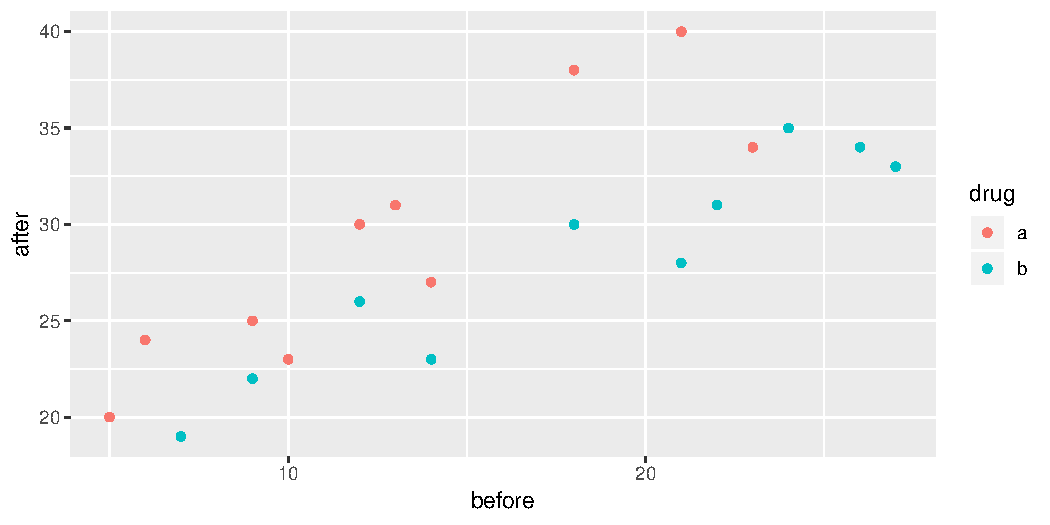
\includegraphics[width=\maxwidth]{figure/spizzo-1} 

\end{knitrout}
  
  
\end{frame}

\begin{frame}[fragile]{Comments}

\begin{knitrout}
\definecolor{shadecolor}{rgb}{0.969, 0.969, 0.969}\color{fgcolor}\begin{kframe}
\begin{alltt}
\hlstd{g}
\end{alltt}
\end{kframe}
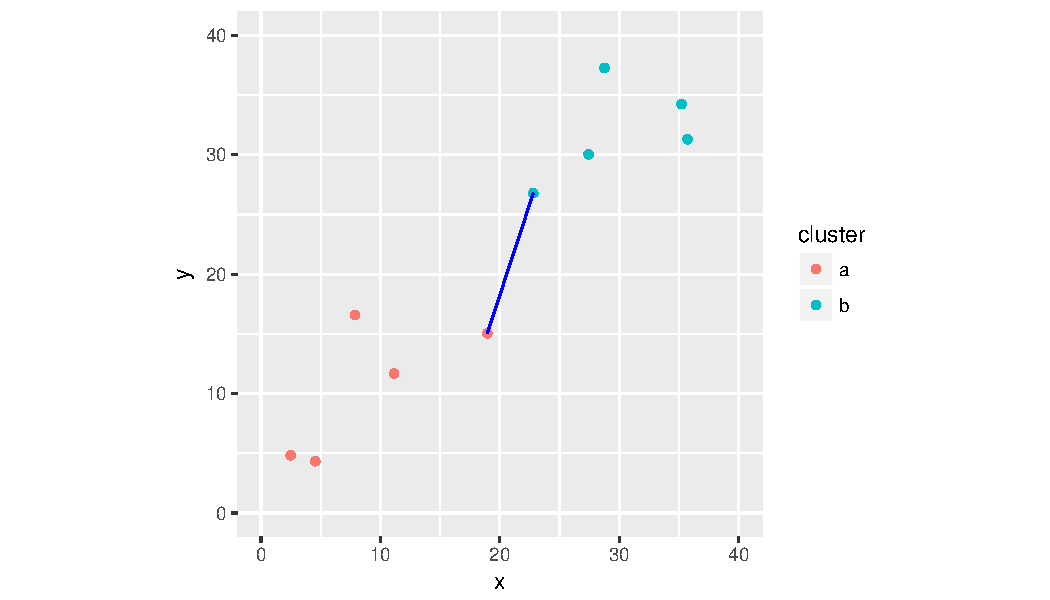
\includegraphics[width=\maxwidth]{figure/unnamed-chunk-3-1} 

\end{knitrout}

\begin{itemize}
\item As before score goes up, after score goes up.
\item Red points (drug A) generally above blue points (drug B), for
  comparable before score.
\item Suggests before score effect \emph{and} drug effect.
\end{itemize}
  
\end{frame}


\begin{frame}[fragile]{The means}

 
\begin{knitrout}
\definecolor{shadecolor}{rgb}{0.969, 0.969, 0.969}\color{fgcolor}\begin{kframe}
\begin{alltt}
\hlstd{prepost} \hlopt \hlkwd{group_by}\hlstd{(drug)} \hlopt
  \hlkwd{summarize}\hlstd{(}\hlkwc{before_mean}\hlstd{=}\hlkwd{mean}\hlstd{(before),}
            \hlkwc{after_mean}\hlstd{=}\hlkwd{mean}\hlstd{(after)}
           \hlstd{)}
\end{alltt}
\begin{verbatim}
## # A tibble: 2 × 3
##     drug before_mean after_mean
##   <fctr>       <dbl>      <dbl>
## 1      a        13.1       29.2
## 2      b        18.0       28.1
\end{verbatim}
\end{kframe}
\end{knitrout}
  

\begin{itemize}
\item Mean ``after'' score slightly higher for treatment A.
\item Mean ``before'' score much higher for treatment B.
\item Greater {\em improvement} on treatment A. 
\end{itemize}
  
\end{frame}

\begin{frame}[fragile]{Testing for interaction}

 
\begin{knitrout}
\definecolor{shadecolor}{rgb}{0.969, 0.969, 0.969}\color{fgcolor}\begin{kframe}
\begin{alltt}
\hlstd{prepost.1}\hlkwb{=}\hlkwd{lm}\hlstd{(after}\hlopt{~}\hlstd{before}\hlopt{*}\hlstd{drug,}\hlkwc{data}\hlstd{=prepost)}
\hlkwd{anova}\hlstd{(prepost.1)}
\end{alltt}
\begin{verbatim}
## Analysis of Variance Table
## 
## Response: after
##             Df Sum Sq Mean Sq F value    Pr(>F)    
## before       1 430.92  430.92 62.6894  6.34e-07 ***
## drug         1 115.31  115.31 16.7743 0.0008442 ***
## before:drug  1  12.34   12.34  1.7948 0.1990662    
## Residuals   16 109.98    6.87                      
## ---
## Signif. codes:  0 '***' 0.001 '**' 0.01 '*' 0.05 '.' 0.1 ' ' 1
\end{verbatim}
\end{kframe}
\end{knitrout}


\begin{itemize}
\item Interaction not significant. Will remove later.
\end{itemize}
\end{frame}



\begin{frame}[fragile]{Predictions, with interaction included}


  
  \begin{multicols}{2}
    

  
  Make combinations of before score and drug:
  
\begin{knitrout}
\definecolor{shadecolor}{rgb}{0.969, 0.969, 0.969}\color{fgcolor}\begin{kframe}
\begin{alltt}
\hlstd{new}\hlkwb{=}\hlkwd{expand.grid}\hlstd{(}
      \hlkwc{before}\hlstd{=}\hlkwd{c}\hlstd{(}\hlnum{5}\hlstd{,}\hlnum{15}\hlstd{,}\hlnum{25}\hlstd{),}
      \hlkwc{drug}\hlstd{=}\hlkwd{c}\hlstd{(}\hlstr{"a"}\hlstd{,}\hlstr{"b"}\hlstd{)}
               \hlstd{)}
\hlstd{new}
\end{alltt}
\begin{verbatim}
##   before drug
## 1      5    a
## 2     15    a
## 3     25    a
## 4      5    b
## 5     15    b
## 6     25    b
\end{verbatim}
\end{kframe}
\end{knitrout}

Do predictions:

\begin{knitrout}
\definecolor{shadecolor}{rgb}{0.969, 0.969, 0.969}\color{fgcolor}\begin{kframe}
\begin{alltt}
\hlstd{pred}\hlkwb{=}\hlkwd{predict}\hlstd{(prepost.1,new)}
\hlstd{preds}\hlkwb{=}\hlkwd{data.frame}\hlstd{(new,pred)}
\hlstd{preds}
\end{alltt}
\begin{verbatim}
##   before drug     pred
## 1      5    a 21.29948
## 2     15    a 31.05321
## 3     25    a 40.80693
## 4      5    b 18.71739
## 5     15    b 25.93478
## 6     25    b 33.15217
\end{verbatim}
\end{kframe}
\end{knitrout}
  
  \end{multicols}

\end{frame}

\begin{frame}[fragile]{Making a plot with lines for each \texttt{drug}}

 
\begin{knitrout}
\definecolor{shadecolor}{rgb}{0.969, 0.969, 0.969}\color{fgcolor}\begin{kframe}
\begin{alltt}
\hlstd{g}\hlkwb{=}\hlkwd{ggplot}\hlstd{(prepost,}
  \hlkwd{aes}\hlstd{(}\hlkwc{x}\hlstd{=before,}\hlkwc{y}\hlstd{=after,}\hlkwc{colour}\hlstd{=drug))}\hlopt{+}
  \hlkwd{geom_point}\hlstd{()}\hlopt{+}
  \hlkwd{geom_line}\hlstd{(}\hlkwc{data}\hlstd{=preds,}\hlkwd{aes}\hlstd{(}\hlkwc{y}\hlstd{=pred))}
\end{alltt}
\end{kframe}
\end{knitrout}


\begin{itemize}
\item Last line could (more easily) be 

\begin{knitrout}
\definecolor{shadecolor}{rgb}{0.969, 0.969, 0.969}\color{fgcolor}\begin{kframe}
\begin{alltt}
\hlkwd{geom_smooth}\hlstd{(}\hlkwc{method}\hlstd{=}\hlstr{"lm"}\hlstd{,}\hlkwc{se}\hlstd{=F)}
\end{alltt}
\end{kframe}
\end{knitrout}

which would work here, but not for later plot.
\item Here, final line:
  \begin{itemize}
  \item   joins points by lines \emph{for different data
    set} (\texttt{preds} rather than \texttt{prepost}),
\item   \emph{different $y$} (\texttt{pred} rather than \texttt{after}),
  
\item but same $x$ (\texttt{x=before} inherited from first \texttt{aes}).

  \end{itemize}
  
\end{itemize}
  
  
\end{frame}

\begin{frame}[fragile]{The plot}
 
  
\begin{knitrout}
\definecolor{shadecolor}{rgb}{0.969, 0.969, 0.969}\color{fgcolor}\begin{kframe}
\begin{alltt}
\hlstd{g}
\end{alltt}
\end{kframe}
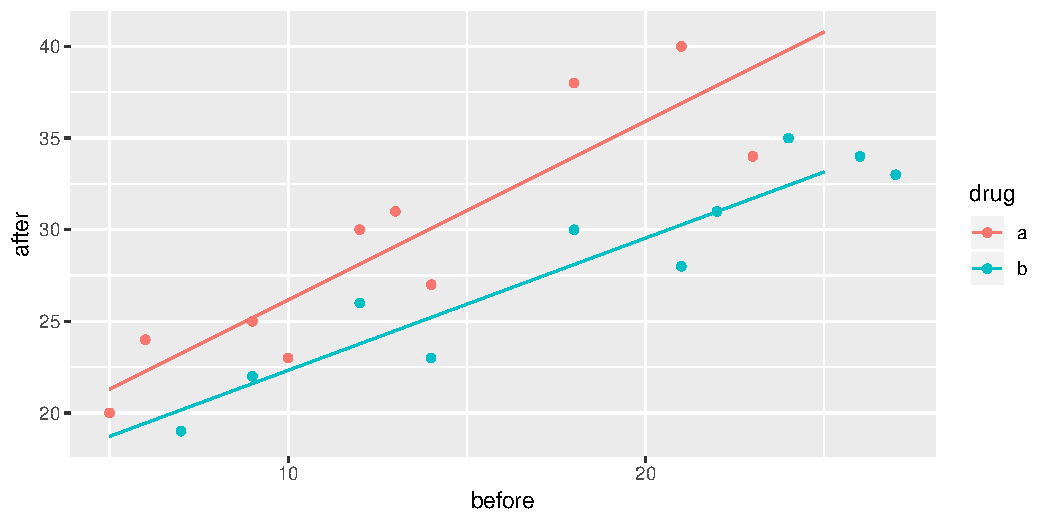
\includegraphics[width=\maxwidth]{figure/nachwazzo-1} 

\end{knitrout}
   
   
 
 \begin{itemize}
 \item Lines almost parallel, but not quite.
 \item Non-parallelism (interaction) not significant.
 \end{itemize}
   
\end{frame}
 

\begin{frame}[fragile]{Taking out interaction}


{\small
  
 
\begin{knitrout}
\definecolor{shadecolor}{rgb}{0.969, 0.969, 0.969}\color{fgcolor}\begin{kframe}
\begin{alltt}
\hlstd{prepost.2}\hlkwb{=}\hlkwd{lm}\hlstd{(after}\hlopt{~}\hlstd{before}\hlopt{+}\hlstd{drug,}\hlkwc{data}\hlstd{=prepost)}
\hlkwd{anova}\hlstd{(prepost.2)}
\end{alltt}
\begin{verbatim}
## Analysis of Variance Table
## 
## Response: after
##           Df Sum Sq Mean Sq F value    Pr(>F)    
## before     1 430.92  430.92  59.890 5.718e-07 ***
## drug       1 115.31  115.31  16.025 0.0009209 ***
## Residuals 17 122.32    7.20                      
## ---
## Signif. codes:  0 '***' 0.001 '**' 0.01 '*' 0.05 '.' 0.1 ' ' 1
\end{verbatim}
\end{kframe}
\end{knitrout}
}
  
  \begin{itemize}
  \item Take out non-significant interaction.
  \item \texttt{before} and \texttt{drug} strongly significant.
  \item Do predictions again and plot them.
  \end{itemize}
  
\end{frame}

\begin{frame}[fragile]{Predicted values again (no-interaction model)}

   
\begin{knitrout}
\definecolor{shadecolor}{rgb}{0.969, 0.969, 0.969}\color{fgcolor}\begin{kframe}
\begin{alltt}
\hlstd{pred}\hlkwb{=}\hlkwd{predict}\hlstd{(prepost.2,new)}
\hlstd{preds}\hlkwb{=}\hlkwd{data.frame}\hlstd{(new,pred)}
\hlstd{preds}
\end{alltt}
\begin{verbatim}
##   before drug     pred
## 1      5    a 22.49740
## 2     15    a 30.77221
## 3     25    a 39.04703
## 4      5    b 17.34274
## 5     15    b 25.61756
## 6     25    b 33.89237
\end{verbatim}
\end{kframe}
\end{knitrout}
 

Each increase of 10 in before score results in 8.3 in predicted after
score, \emph{the same for both drugs}.
  
\end{frame}

\begin{frame}[fragile]{Making a plot, again}

 
\begin{knitrout}
\definecolor{shadecolor}{rgb}{0.969, 0.969, 0.969}\color{fgcolor}\begin{kframe}
\begin{alltt}
\hlstd{g}\hlkwb{=}\hlkwd{ggplot}\hlstd{(prepost,}
  \hlkwd{aes}\hlstd{(}\hlkwc{x}\hlstd{=before,}\hlkwc{y}\hlstd{=after,}\hlkwc{colour}\hlstd{=drug))}\hlopt{+}
  \hlkwd{geom_point}\hlstd{()}\hlopt{+}
  \hlkwd{geom_line}\hlstd{(}\hlkwc{data}\hlstd{=preds,}\hlkwd{aes}\hlstd{(}\hlkwc{y}\hlstd{=pred))}
\end{alltt}
\end{kframe}
\end{knitrout}
 

Exactly same as before, but using new predictions.
  
\end{frame}

\begin{frame}{The no-interaction plot of predicted values}
  
 
\begin{knitrout}
\definecolor{shadecolor}{rgb}{0.969, 0.969, 0.969}\color{fgcolor}\begin{kframe}
\begin{alltt}
\hlstd{g}
\end{alltt}
\end{kframe}
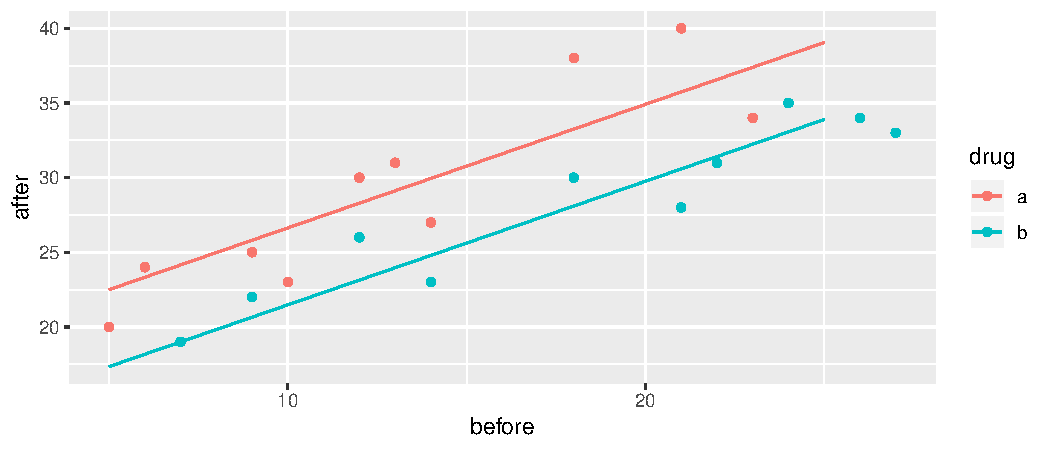
\includegraphics[width=\maxwidth]{figure/cabazzo-1} 

\end{knitrout}


Note that lines now \emph{parallel}. No-interaction model forces them
to have the same slope. 

\end{frame}

\begin{frame}[fragile]{Different look at model output}
  
  \begin{itemize}
  \item \texttt{anova(prepost.2)} tests for significant effect of
    before score and of drug, but doesn't help with interpretation.
  \item \texttt{summary(prepost.2)} views as regression with slopes:
    
    \begin{scriptsize}
\begin{knitrout}
\definecolor{shadecolor}{rgb}{0.969, 0.969, 0.969}\color{fgcolor}\begin{kframe}
\begin{alltt}
\hlkwd{summary}\hlstd{(prepost.2)}
\end{alltt}
\begin{verbatim}
## 
## Call:
## lm(formula = after ~ before + drug, data = prepost)
## 
## Residuals:
##     Min      1Q  Median      3Q     Max 
## -3.6348 -2.5099 -0.2038  1.8871  4.7453 
## 
## Coefficients:
##             Estimate Std. Error t value Pr(>|t|)    
## (Intercept)  18.3600     1.5115  12.147 8.35e-10 ***
## before        0.8275     0.0955   8.665 1.21e-07 ***
## drugb        -5.1547     1.2876  -4.003 0.000921 ***
## ---
## Signif. codes:  0 '***' 0.001 '**' 0.01 '*' 0.05 '.' 0.1 ' ' 1
## 
## Residual standard error: 2.682 on 17 degrees of freedom
## Multiple R-squared:  0.817,	Adjusted R-squared:  0.7955 
## F-statistic: 37.96 on 2 and 17 DF,  p-value: 5.372e-07
\end{verbatim}
\end{kframe}
\end{knitrout}
    \end{scriptsize}
  \end{itemize}
  
\end{frame}

\begin{frame}[fragile]{Understanding those slopes}
  
  \begin{scriptsize}
\begin{knitrout}
\definecolor{shadecolor}{rgb}{0.969, 0.969, 0.969}\color{fgcolor}\begin{kframe}
\begin{alltt}
\hlkwd{summary}\hlstd{(prepost.2)}\hlopt{$}\hlstd{coefficients}
\end{alltt}
\begin{verbatim}
##               Estimate Std. Error   t value     Pr(>|t|)
## (Intercept) 18.3599949 1.51153263 12.146608 8.354496e-10
## before       0.8274813 0.09550226  8.664520 1.211339e-07
## drugb       -5.1546584 1.28765245 -4.003144 9.209111e-04
\end{verbatim}
\end{kframe}
\end{knitrout}
%$ %$ %$
  \end{scriptsize}

\begin{itemize}
\item \texttt{before} ordinary numerical variable; \texttt{drug}
  categorical. 
\item \texttt{lm} uses first category \texttt{druga} as baseline.
\item Intercept is prediction of after score for before score 0 and
  \emph{drug A}.
\item \texttt{before} slope is predicted change in after score when
  before score increases by 1 (usual slope)
\item Slope for \texttt{drugb} is \emph{change} in predicted after
  score for being on drug B rather than drug A. Same for \emph{any}
  before score (no interaction).
\item In \texttt{summary(prepost.1)}, \texttt{before:drugb} would be change in
  \emph{slope} for being on drug B rather than A.
  
\end{itemize}

  
\end{frame}

\begin{frame}[fragile]{Summary}

  \begin{itemize}
  \item ANCOVA model: fits different regression line for each group,
    predicting response from covariate.
  \item ANCOVA model with interaction between factor and covariate
    allows different slopes for each line.
  \item Sometimes those lines can cross over!
  \item If interaction not significant, take out. Lines then parallel.
  \item With parallel lines, groups have consistent effect regardless
    of value of covariate.
  \end{itemize}
  
\end{frame}

\section{Multivariate ANOVA}
\frame{\sectionpage}


\begin{frame}[fragile]{Multivariate analysis of variance}

  \begin{itemize}
  \item Standard ANOVA has just one response variable.
  \item What if you have more than one response?
  \item Try an ANOVA on each response separately.
  \item But might miss some kinds of interesting dependence between the responses that distinguish the groups.
  \end{itemize}
  
\end{frame}

\begin{frame}[fragile]{Small example}

  \begin{itemize}
  \item Measure yield and seed weight of plants grown under 2 conditions: low and high amounts of fertilizer.
  \item Data (fertilizer, yield, seed weight):


 
\begin{knitrout}
\definecolor{shadecolor}{rgb}{0.969, 0.969, 0.969}\color{fgcolor}\begin{kframe}
\begin{alltt}
\hlstd{hilo}\hlkwb{=}\hlkwd{read.table}\hlstd{(}\hlstr{"manova1.txt"}\hlstd{,}\hlkwc{header}\hlstd{=T)}
\hlstd{hilo}
\end{alltt}
\begin{verbatim}
##   fertilizer yield weight
## 1        low    34     10
## 2        low    29     14
## 3        low    35     11
## 4        low    32     13
## 5       high    33     14
## 6       high    38     12
## 7       high    34     13
## 8       high    35     14
\end{verbatim}
\end{kframe}
\end{knitrout}

  \item 2 responses, yield and seed weight.
  \end{itemize}
  
\end{frame}

\begin{frame}[fragile]{Boxplot for yield for each fertilizer group}

 
\begin{knitrout}
\definecolor{shadecolor}{rgb}{0.969, 0.969, 0.969}\color{fgcolor}\begin{kframe}
\begin{alltt}
\hlkwd{ggplot}\hlstd{(hilo,}\hlkwd{aes}\hlstd{(}\hlkwc{x}\hlstd{=fertilizer,}\hlkwc{y}\hlstd{=yield))}\hlopt{+}\hlkwd{geom_boxplot}\hlstd{()}
\end{alltt}
\end{kframe}
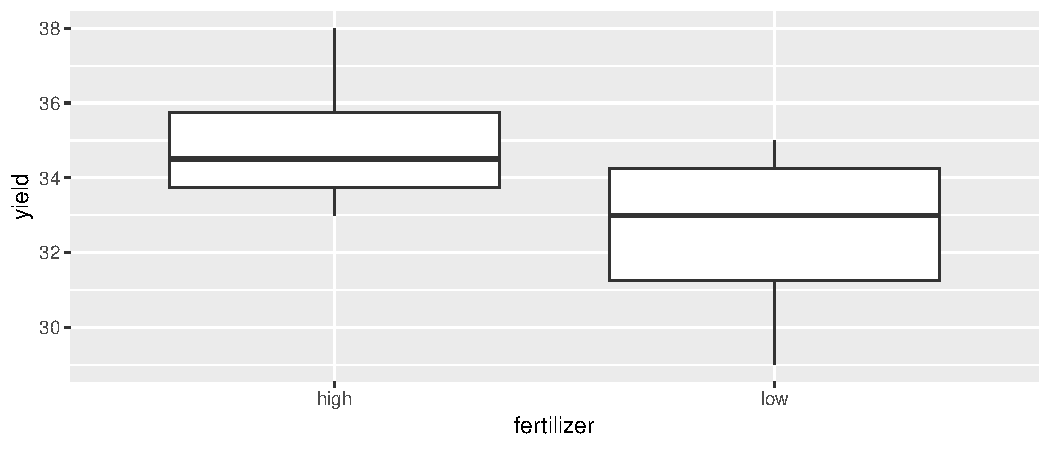
\includegraphics[width=\maxwidth]{figure/ferto-1} 

\end{knitrout}
  
  

Yields overlap for fertilizer groups.
  
\end{frame}

\begin{frame}[fragile]{Boxplot for weight for each fertilizer group}

 
\begin{knitrout}
\definecolor{shadecolor}{rgb}{0.969, 0.969, 0.969}\color{fgcolor}\begin{kframe}
\begin{alltt}
\hlkwd{ggplot}\hlstd{(hilo,}\hlkwd{aes}\hlstd{(}\hlkwc{x}\hlstd{=fertilizer,}\hlkwc{y}\hlstd{=weight))}\hlopt{+}\hlkwd{geom_boxplot}\hlstd{()}
\end{alltt}
\end{kframe}
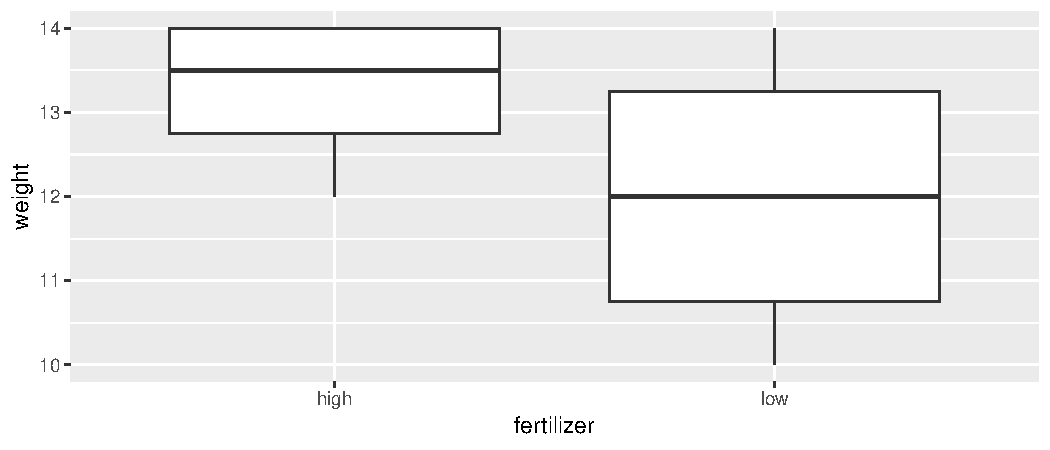
\includegraphics[width=\maxwidth]{figure/casteldisangro-1} 

\end{knitrout}

Weights overlap for fertilizer groups.
  
\end{frame}

\begin{frame}[fragile]{ANOVAs for yield and weight}

{\small
 
\begin{knitrout}
\definecolor{shadecolor}{rgb}{0.969, 0.969, 0.969}\color{fgcolor}\begin{kframe}
\begin{alltt}
\hlstd{hilo.y}\hlkwb{=}\hlkwd{aov}\hlstd{(yield}\hlopt{~}\hlstd{fertilizer,}\hlkwc{data}\hlstd{=hilo)}
\hlkwd{summary}\hlstd{(hilo.y)}
\end{alltt}
\begin{verbatim}
##             Df Sum Sq Mean Sq F value Pr(>F)
## fertilizer   1   12.5  12.500   2.143  0.194
## Residuals    6   35.0   5.833
\end{verbatim}
\begin{alltt}
\hlstd{hilo.w}\hlkwb{=}\hlkwd{aov}\hlstd{(weight}\hlopt{~}\hlstd{fertilizer,}\hlkwc{data}\hlstd{=hilo)}
\hlkwd{summary}\hlstd{(hilo.w)}
\end{alltt}
\begin{verbatim}
##             Df Sum Sq Mean Sq F value Pr(>F)
## fertilizer   1  3.125   3.125   1.471  0.271
## Residuals    6 12.750   2.125
\end{verbatim}
\end{kframe}
\end{knitrout}
}

Neither response depends significantly on fertilizer. But\ldots
  
\end{frame}

\begin{frame}[fragile]{Plotting both responses at once}

Have two response variables (not more), so can plot the
response variables against \emph{each other}, labelling points by
which fertilizer group they're from.

\begin{knitrout}
\definecolor{shadecolor}{rgb}{0.969, 0.969, 0.969}\color{fgcolor}\begin{kframe}
\begin{alltt}
\hlstd{g}\hlkwb{=}\hlkwd{ggplot}\hlstd{(hilo,}\hlkwd{aes}\hlstd{(}\hlkwc{x}\hlstd{=yield,}\hlkwc{y}\hlstd{=weight,}\hlkwc{colour}\hlstd{=fertilizer))}\hlopt{+}
  \hlkwd{geom_point}\hlstd{()}
\end{alltt}
\end{kframe}
\end{knitrout}

Also want line through
points $(31,14)$ and $(38,10)$ (see why later):

\begin{knitrout}
\definecolor{shadecolor}{rgb}{0.969, 0.969, 0.969}\color{fgcolor}\begin{kframe}
\begin{alltt}
\hlstd{line_x}\hlkwb{=}\hlkwd{c}\hlstd{(}\hlnum{31}\hlstd{,}\hlnum{38}\hlstd{)}
\hlstd{line_y}\hlkwb{=}\hlkwd{c}\hlstd{(}\hlnum{14}\hlstd{,}\hlnum{10}\hlstd{)}
\hlstd{d}\hlkwb{=}\hlkwd{data.frame}\hlstd{(line_x,line_y)}
\hlstd{g}\hlkwb{=}\hlstd{g}\hlopt{+}\hlkwd{geom_smooth}\hlstd{(}\hlkwc{data}\hlstd{=d,}\hlkwd{aes}\hlstd{(}\hlkwc{x}\hlstd{=line_x,}\hlkwc{y}\hlstd{=line_y,}\hlkwc{colour}\hlstd{=}\hlkwa{NULL}\hlstd{),}
  \hlkwc{method}\hlstd{=}\hlstr{"lm"}\hlstd{,}\hlkwc{se}\hlstd{=F)}
\end{alltt}
\end{kframe}
\end{knitrout}

I am fitting a regression line through the points in \texttt{d}. I am
adding to a previous \texttt{ggplot}, so my \texttt{geom\_smooth} is
inheriting the \texttt{colour} from the first one. This data frame has
no \texttt{fertilizer} (what previous \texttt{colour} was), so I have to unset it.
  
\end{frame}

\begin{frame}[fragile]{The plot}
  
 
\begin{knitrout}
\definecolor{shadecolor}{rgb}{0.969, 0.969, 0.969}\color{fgcolor}\begin{kframe}
\begin{alltt}
\hlstd{g}
\end{alltt}
\end{kframe}
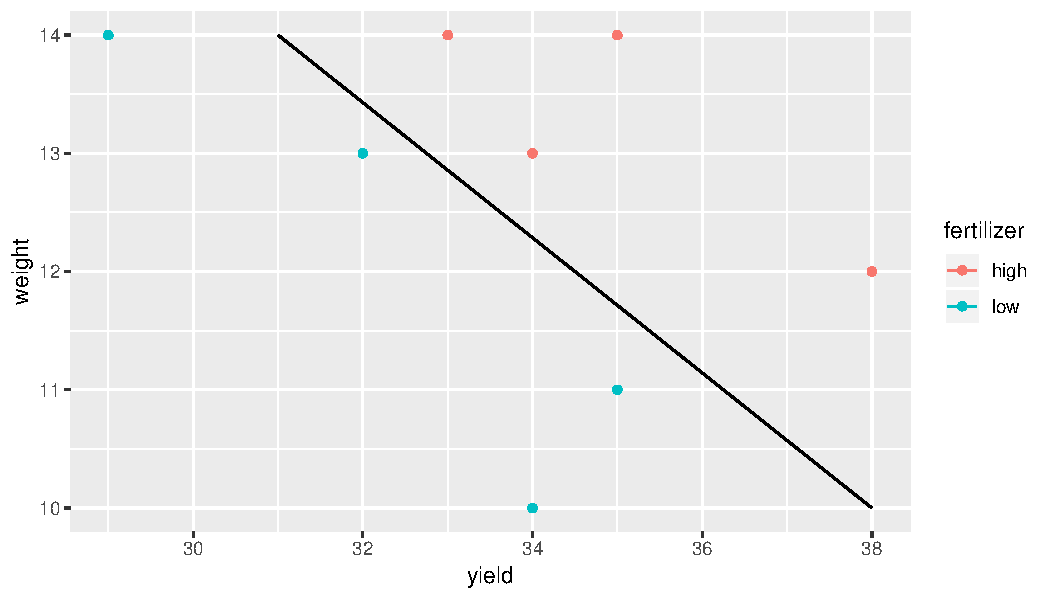
\includegraphics[width=\maxwidth]{figure/charlecombe-1} 

\end{knitrout}
  
  
\end{frame}

\begin{frame}[fragile]{MANOVA}
  
\begin{knitrout}
\definecolor{shadecolor}{rgb}{0.969, 0.969, 0.969}\color{fgcolor}\begin{kframe}
\begin{alltt}
\hlstd{g}
\end{alltt}
\end{kframe}
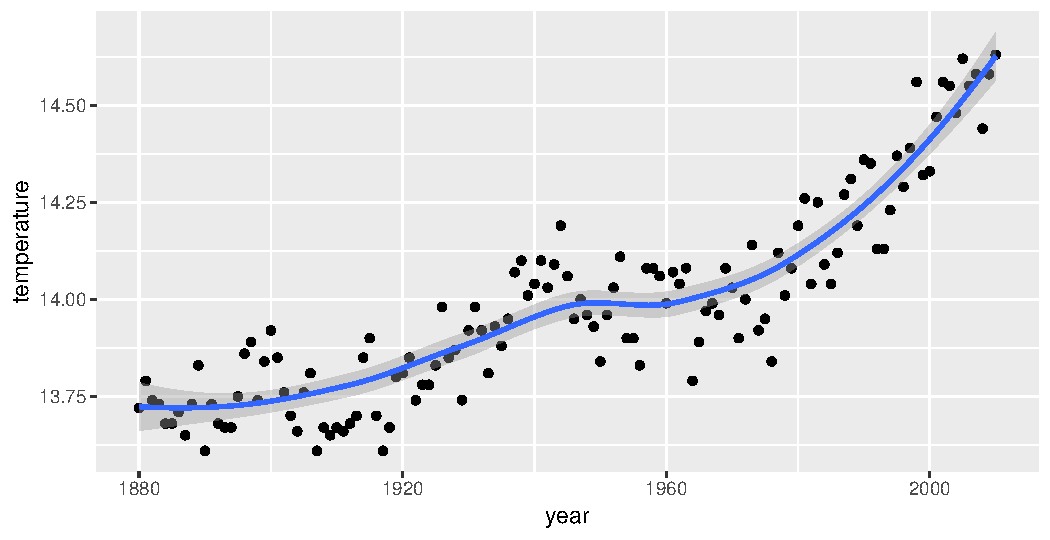
\includegraphics[width=\maxwidth]{figure/unnamed-chunk-6-1} 

\end{knitrout}
  \begin{itemize}
  \item High-fertilizer plants have both yield and weight high.
  \item True even though no sig difference in yield or weight individually.
  \item Drew line separating highs from lows on plot.
  \end{itemize}

 

\end{frame}

\begin{frame}[fragile]{MANOVA finds multivariate differences}
  
  \begin{itemize}
  \item Is difference found by diagonal line significant? MANOVA finds out.

  \end{itemize}

  \begin{small}
\begin{knitrout}
\definecolor{shadecolor}{rgb}{0.969, 0.969, 0.969}\color{fgcolor}\begin{kframe}
\begin{alltt}
\hlstd{response}\hlkwb{=}\hlkwd{with}\hlstd{(hilo,}\hlkwd{cbind}\hlstd{(yield,weight))}
\hlstd{hilo.1}\hlkwb{=}\hlkwd{manova}\hlstd{(response}\hlopt{~}\hlstd{fertilizer,}\hlkwc{data}\hlstd{=hilo)}
\hlkwd{summary}\hlstd{(hilo.1)}
\end{alltt}
\begin{verbatim}
##            Df  Pillai approx F num Df den Df  Pr(>F)  
## fertilizer  1 0.80154   10.097      2      5 0.01755 *
## Residuals   6                                         
## ---
## Signif. codes:  0 '***' 0.001 '**' 0.01 '*' 0.05 '.' 0.1 ' ' 1
\end{verbatim}
\end{kframe}
\end{knitrout}
    
  \end{small}

Yes! Difference between groups is \emph{diagonally}, not just up/down
(weight) or left-right (yield). The \emph{yield-weight combination} matters.
  
\end{frame}

\begin{frame}[fragile]{Strategy}

\begin{itemize}
\item Create new response variable by gluing together columns of
  responses, using \texttt{cbind}.
\item Use \texttt{manova} with new response, looks like \texttt{lm} otherwise.
\item With more than 2 responses, cannot draw graph. What then?
\item If MANOVA test significant, cannot use Tukey. What then?
\item Use {\em discriminant analysis} (of which more later).
\end{itemize}

\end{frame}

\begin{frame}[fragile]{Another way to do MANOVA}

  
  \begin{itemize}
  \item Install package \texttt{car}, then:
  
{\small
 
\begin{knitrout}
\definecolor{shadecolor}{rgb}{0.969, 0.969, 0.969}\color{fgcolor}\begin{kframe}
\begin{alltt}
\hlstd{hilo.2.lm}\hlkwb{=}\hlkwd{lm}\hlstd{(response}\hlopt{~}\hlstd{fertilizer,}\hlkwc{data}\hlstd{=hilo)}
\hlstd{hilo.2}\hlkwb{=}\hlstd{car}\hlopt{::}\hlkwd{Manova}\hlstd{(hilo.2.lm)}
\hlstd{hilo.2}
\end{alltt}
\begin{verbatim}
## 
## Type II MANOVA Tests: Pillai test statistic
##            Df test stat approx F num Df den Df  Pr(>F)  
## fertilizer  1   0.80154   10.097      2      5 0.01755 *
## ---
## Signif. codes:  0 '***' 0.001 '**' 0.01 '*' 0.05 '.' 0.1 ' ' 1
\end{verbatim}
\end{kframe}
\end{knitrout}

}

  
\item Or \texttt{library(car)} followed by \texttt{Manova(...)}.
\item Same result as small-m \texttt{manova}.
\item \texttt{Manova} will also do \emph{repeated measures}, coming up.
\end{itemize}
  
\end{frame}

\begin{frame}[fragile]{Another example: peanuts}

  \begin{itemize}
  \item  Three different varieties
of peanuts (mysteriously, 5, 6 and 8) planted in two different
locations.
\item Three response variables: \texttt{y}, \texttt{smk} and
\texttt{w}.
  \end{itemize}

 
\begin{knitrout}
\definecolor{shadecolor}{rgb}{0.969, 0.969, 0.969}\color{fgcolor}\begin{kframe}
\begin{alltt}
\hlstd{peanuts.orig}\hlkwb{=}\hlkwd{read.table}\hlstd{(}\hlstr{"peanuts.txt"}\hlstd{,}\hlkwc{header}\hlstd{=T)}
\hlkwd{head}\hlstd{(peanuts.orig)}
\end{alltt}
\begin{verbatim}
##   obs location variety     y   smk    w
## 1   1        1       5 195.3 153.1 51.4
## 2   2        1       5 194.3 167.7 53.7
## 3   3        2       5 189.7 139.5 55.5
## 4   4        2       5 180.4 121.1 44.4
## 5   5        1       6 203.0 156.8 49.8
## 6   6        1       6 195.9 166.0 45.8
\end{verbatim}
\end{kframe}
\end{knitrout}
    
    
\end{frame}

\begin{frame}[fragile]{Setup for analysis}

  Using \texttt{dplyr}:
 
\begin{knitrout}
\definecolor{shadecolor}{rgb}{0.969, 0.969, 0.969}\color{fgcolor}\begin{kframe}
\begin{alltt}
\hlstd{peanuts.orig} \hlopt
  \hlkwd{mutate}\hlstd{(}\hlkwc{location}\hlstd{=}\hlkwd{factor}\hlstd{(location),}
         \hlkwc{variety}\hlstd{=}\hlkwd{factor}\hlstd{(variety))} \hlkwb{->} \hlstd{peanuts}
\hlstd{response}\hlkwb{=}\hlkwd{with}\hlstd{(peanuts,}\hlkwd{cbind}\hlstd{(y,smk,w))}
\hlkwd{head}\hlstd{(response)}
\end{alltt}
\begin{verbatim}
##          y   smk    w
## [1,] 195.3 153.1 51.4
## [2,] 194.3 167.7 53.7
## [3,] 189.7 139.5 55.5
## [4,] 180.4 121.1 44.4
## [5,] 203.0 156.8 49.8
## [6,] 195.9 166.0 45.8
\end{verbatim}
\end{kframe}
\end{knitrout}

  
\end{frame}

\begin{frame}[fragile]{Analysis (using \texttt{Manova})}

{\footnotesize  
 
\begin{knitrout}
\definecolor{shadecolor}{rgb}{0.969, 0.969, 0.969}\color{fgcolor}\begin{kframe}
\begin{alltt}
\hlstd{peanuts.1}\hlkwb{=}\hlkwd{lm}\hlstd{(response}\hlopt{~}\hlstd{location}\hlopt{*}\hlstd{variety,}\hlkwc{data}\hlstd{=peanuts)}
\hlstd{peanuts.2}\hlkwb{=}\hlstd{car}\hlopt{::}\hlkwd{Manova}\hlstd{(peanuts.1)}
\hlstd{peanuts.2}
\end{alltt}
\begin{verbatim}
## 
## Type II MANOVA Tests: Pillai test statistic
##                  Df test stat approx F num Df den Df   Pr(>F)   
## location          1   0.89348  11.1843      3      4 0.020502 * 
## variety           2   1.70911   9.7924      6     10 0.001056 **
## location:variety  2   1.29086   3.0339      6     10 0.058708 . 
## ---
## Signif. codes:  0 '***' 0.001 '**' 0.01 '*' 0.05 '.' 0.1 ' ' 1
\end{verbatim}
\end{kframe}
\end{knitrout}
}  

\begin{itemize}
\item Interaction not quite significant, but main effects are.
\item Combined response variable \texttt{(y,smk,w)} definitely depends
  on location and on variety
\item Weak dependence of \texttt{(y,smk,w)} on the location-variety \emph{combination.}
\item Understanding that dependence beyond our scope right now.
\end{itemize}

  
\end{frame}

\section{Repeated measures by profile analysis}
\frame{\sectionpage}

\begin{frame}[fragile]{Repeated measures by profile analysis}

  \begin{itemize}
  \item More than one response {\em measurement} for each subject. Might be
    \begin{itemize}
    \item measurements of the same thing at different times
    \item measurements of different but related things
    \end{itemize}
  \item Generalization of matched pairs (``matched triples'', etc.).
  \item Variation: each subject does several different treatments at different times (called {\em crossover design}).
  \item Expect measurements on same subject to be correlated, so
    assumptions of independence will fail.
  \item Called {\em repeated measures}. Different approaches, but {\em
      profile analysis} uses \texttt{Manova} (set up right way).
  \item Another approach uses \emph{mixed models} (random effects).
  \end{itemize}
\end{frame}




\begin{frame}[fragile]{Example: histamine in dogs}
  
  \begin{itemize}
  \item 8 dogs take part in experiment.
  \item Dogs randomized to one of 2 different drugs.
  \item Response: log of blood concentration of histamine 0, 1, 3 and 5 minutes after taking drug. (Repeated measures.)
  \item Data in dogs.txt.
  \end{itemize}

\end{frame}

\begin{frame}[fragile]{Setting things up}


 
\begin{knitrout}
\definecolor{shadecolor}{rgb}{0.969, 0.969, 0.969}\color{fgcolor}\begin{kframe}
\begin{alltt}
\hlstd{dogs}\hlkwb{=}\hlkwd{read.table}\hlstd{(}\hlstr{"dogs.txt"}\hlstd{,}\hlkwc{header}\hlstd{=T)}
\hlstd{dogs}
\end{alltt}
\begin{verbatim}
##   dog         drug x   lh0   lh1   lh3   lh5
## 1   A     Morphine N -3.22 -1.61 -2.30 -2.53
## 2   B     Morphine N -3.91 -2.81 -3.91 -3.91
## 3   C     Morphine N -2.66  0.34 -0.73 -1.43
## 4   D     Morphine N -1.77 -0.56 -1.05 -1.43
## 5   E Trimethaphan N -3.51 -0.48 -1.17 -1.51
## 6   F Trimethaphan N -3.51  0.05 -0.31 -0.51
## 7   G Trimethaphan N -2.66 -0.19  0.07 -0.22
## 8   H Trimethaphan N -2.41  1.14  0.72  0.21
\end{verbatim}
\begin{alltt}
\hlstd{response}\hlkwb{=}\hlkwd{with}\hlstd{(dogs,}\hlkwd{cbind}\hlstd{(lh0,lh1,lh3,lh5))}
\hlstd{dogs.lm}\hlkwb{=}\hlkwd{lm}\hlstd{(response}\hlopt{~}\hlstd{drug,}\hlkwc{data}\hlstd{=dogs)}
\end{alltt}
\end{kframe}
\end{knitrout}
  
    
\end{frame}

\begin{frame}[fragile]{The repeated measures MANOVA}

Get list of response variable names; we call them \texttt{times}. Save
in data frame.

{\footnotesize
 
\begin{knitrout}
\definecolor{shadecolor}{rgb}{0.969, 0.969, 0.969}\color{fgcolor}\begin{kframe}
\begin{alltt}
\hlstd{times}\hlkwb{=}\hlkwd{colnames}\hlstd{(response)}
\hlstd{times.df}\hlkwb{=}\hlkwd{data.frame}\hlstd{(times)}
\hlstd{dogs.manova}\hlkwb{=}\hlstd{car}\hlopt{::}\hlkwd{Manova}\hlstd{(dogs.lm,}\hlkwc{idata}\hlstd{=times.df,}
     \hlkwc{idesign}\hlstd{=}\hlopt{~}\hlstd{times)}
\hlstd{dogs.manova}
\end{alltt}
\begin{verbatim}
## 
## Type II Repeated Measures MANOVA Tests: Pillai test statistic
##             Df test stat approx F num Df den Df   Pr(>F)   
## (Intercept)  1   0.76347  19.3664      1      6 0.004565 **
## drug         1   0.34263   3.1272      1      6 0.127406   
## times        1   0.94988  25.2690      3      4 0.004631 **
## drug:times   1   0.89476  11.3362      3      4 0.020023 * 
## ---
## Signif. codes:  0 '***' 0.001 '**' 0.01 '*' 0.05 '.' 0.1 ' ' 1
\end{verbatim}
\end{kframe}
\end{knitrout}
}

Interaction significant. Pattern of response over time different
for the two drugs.
\end{frame}

\begin{frame}[fragile]{Wide and long format}

  \begin{itemize}
  \item Want to investigate interaction.
  \item But data frame has several observations per line (``wide format''):
 
\begin{knitrout}
\definecolor{shadecolor}{rgb}{0.969, 0.969, 0.969}\color{fgcolor}\begin{kframe}
\begin{alltt}
\hlkwd{head}\hlstd{(dogs,}\hlkwc{n}\hlstd{=}\hlnum{5}\hlstd{)}
\end{alltt}
\begin{verbatim}
##   dog         drug x   lh0   lh1   lh3   lh5
## 1   A     Morphine N -3.22 -1.61 -2.30 -2.53
## 2   B     Morphine N -3.91 -2.81 -3.91 -3.91
## 3   C     Morphine N -2.66  0.34 -0.73 -1.43
## 4   D     Morphine N -1.77 -0.56 -1.05 -1.43
## 5   E Trimethaphan N -3.51 -0.48 -1.17 -1.51
\end{verbatim}
\end{kframe}
\end{knitrout}
    
  \item Plotting works with data in ``long format'':
    one response per line.
  \item The responses are log-histamine at different times, labelled
    \texttt{lh}-something. Call them all \texttt{lh} and put them in
    one column, with the time they belong to labelled.
  \end{itemize}
  
\end{frame}


\begin{frame}[fragile]{Running \texttt{gather}, try 1}
  
  \texttt{gather} needs: name for thing that makes columns different
  (time), name for thing that makes columns same (they are all values
  of log-histamine), and columns to combine:

  {\small
\begin{knitrout}
\definecolor{shadecolor}{rgb}{0.969, 0.969, 0.969}\color{fgcolor}\begin{kframe}
\begin{alltt}
\hlstd{dogs} \hlopt \hlkwd{gather}\hlstd{(time,lh,lh0}\hlopt{:}\hlstd{lh5)} \hlopt \hlkwd{head}\hlstd{(}\hlnum{12}\hlstd{)}
\end{alltt}
\begin{verbatim}
##    dog         drug x time    lh
## 1    A     Morphine N  lh0 -3.22
## 2    B     Morphine N  lh0 -3.91
## 3    C     Morphine N  lh0 -2.66
## 4    D     Morphine N  lh0 -1.77
## 5    E Trimethaphan N  lh0 -3.51
## 6    F Trimethaphan N  lh0 -3.51
## 7    G Trimethaphan N  lh0 -2.66
## 8    H Trimethaphan N  lh0 -2.41
## 9    A     Morphine N  lh1 -1.61
## 10   B     Morphine N  lh1 -2.81
## 11   C     Morphine N  lh1  0.34
## 12   D     Morphine N  lh1 -0.56
\end{verbatim}
\end{kframe}
\end{knitrout}
}
  
\end{frame}

\begin{frame}[fragile]{Splitting off the times}
  
Not quite right: for the times, we want just the numbers, not the
letters \texttt{lh} every time. Want new variable
containing just number in \texttt{time}:
\texttt{parse\_number}. (Actually  lives in \texttt{readr}, so
\texttt{library(tidyverse)} right way to go.)

{\small
\begin{knitrout}
\definecolor{shadecolor}{rgb}{0.969, 0.969, 0.969}\color{fgcolor}\begin{kframe}
\begin{alltt}
\hlstd{dogs} \hlopt \hlkwd{gather}\hlstd{(timex,lh,lh0}\hlopt{:}\hlstd{lh5)} \hlopt
    \hlkwd{mutate}\hlstd{(}\hlkwc{time}\hlstd{=}\hlkwd{parse_number}\hlstd{(timex))} \hlopt \hlkwd{head}\hlstd{(}\hlnum{10}\hlstd{)}
\end{alltt}
\begin{verbatim}
##    dog         drug x timex    lh time
## 1    A     Morphine N   lh0 -3.22    0
## 2    B     Morphine N   lh0 -3.91    0
## 3    C     Morphine N   lh0 -2.66    0
## 4    D     Morphine N   lh0 -1.77    0
## 5    E Trimethaphan N   lh0 -3.51    0
## 6    F Trimethaphan N   lh0 -3.51    0
## 7    G Trimethaphan N   lh0 -2.66    0
## 8    H Trimethaphan N   lh0 -2.41    0
## 9    A     Morphine N   lh1 -1.61    1
## 10   B     Morphine N   lh1 -2.81    1
\end{verbatim}
\end{kframe}
\end{knitrout}
}

\end{frame}

\begin{frame}[fragile]{What I did differently}
  
  \begin{itemize}
  \item I realized that \texttt{gather} was going to produce something
    like \texttt{lh1}, which I needed to do something further with, so
    this time I gave it a temporary name \texttt{timex}.
  \item This enabled me to use the name \texttt{time} for the actual
    numeric time.
  \item This works now, so next save into a new data frame \texttt{dogs.long}.
  \end{itemize}
  
\end{frame}

\begin{frame}[fragile]{Saving the chained results}
  

\begin{knitrout}
\definecolor{shadecolor}{rgb}{0.969, 0.969, 0.969}\color{fgcolor}\begin{kframe}
\begin{alltt}
\hlstd{dogs} \hlopt \hlkwd{gather}\hlstd{(timex,lh,lh0}\hlopt{:}\hlstd{lh5)} \hlopt
    \hlkwd{mutate}\hlstd{(}\hlkwc{time}\hlstd{=}\hlkwd{parse_number}\hlstd{(timex))}  \hlkwb{->} \hlstd{dogs.long}
\end{alltt}
\end{kframe}
\end{knitrout}

This says:

\begin{itemize}
\item Take data frame dogs, and then:
\item Combine the columns \texttt{lh0} through \texttt{lh5} into one
  column called \texttt{lh}, with the column that each \texttt{lh}
  value originally came from labelled by \texttt{timex}, and then:
\item Pull out numeric values in \texttt{timex}, saving in \texttt{time} and then:
\item save the result in a data frame \texttt{dogs.long}.
\end{itemize}
  
\end{frame}

%
%\begin{frame}[fragile]{\texttt{reshape}}
%
%  \begin{itemize}
%  \item Converts between wide and long format.
%  \item Need to tell R what our repeated-measures responses are.
%  \item Convenient variable naming: all responses are \texttt{lh}
%    followed by a number representing time.
%  \item Like this:
%  \end{itemize}
%
% 
%<<>>=
%detach(dogs)
%d2=reshape(dogs,varying=3:6,sep="",
%    direction="long")
%@ %def 
%
%\end{frame}
%
%\begin{frame}[fragile]{Long data frame, top 12 lines}
%
% 
%<<>>=
%head(d2,n=12)
%@ %def 
%  
%
%\texttt{id}  labels dog, \texttt{time} labels time. Perfect for
%interaction plot.
%  
%\end{frame}
%

\begin{frame}[fragile]{Interaction plot}
  
\begin{knitrout}
\definecolor{shadecolor}{rgb}{0.969, 0.969, 0.969}\color{fgcolor}\begin{kframe}
\begin{alltt}
\hlkwd{ggplot}\hlstd{(dogs.long,}\hlkwd{aes}\hlstd{(}\hlkwc{x}\hlstd{=time,}\hlkwc{y}\hlstd{=lh,}\hlkwc{colour}\hlstd{=drug,}\hlkwc{group}\hlstd{=drug))}\hlopt{+}
  \hlkwd{stat_summary}\hlstd{(}\hlkwc{fun.y}\hlstd{=mean,}\hlkwc{geom}\hlstd{=}\hlstr{"point"}\hlstd{)}\hlopt{+}
  \hlkwd{stat_summary}\hlstd{(}\hlkwc{fun.y}\hlstd{=mean,}\hlkwc{geom}\hlstd{=}\hlstr{"line"}\hlstd{)}
\end{alltt}
\end{kframe}
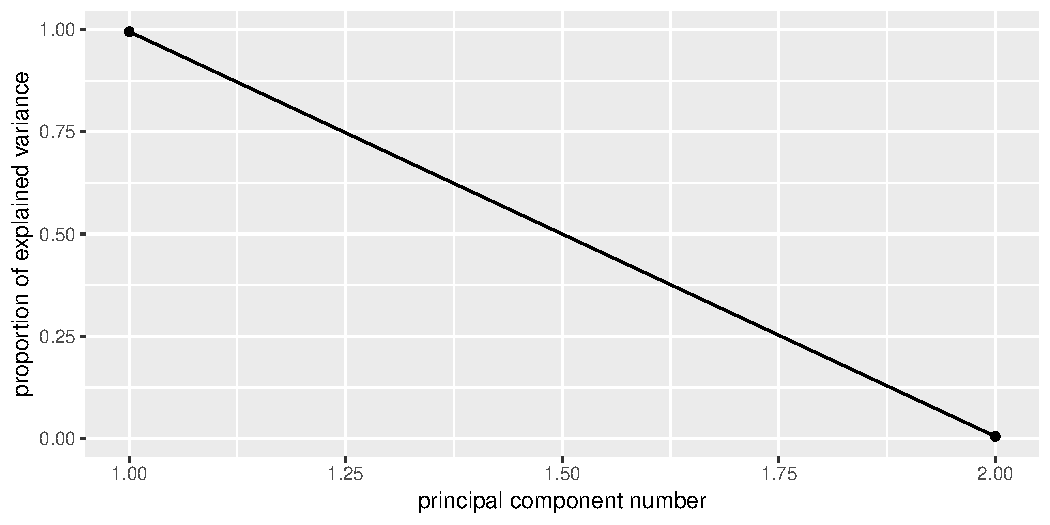
\includegraphics[width=\maxwidth]{figure/unnamed-chunk-8-1} 

\end{knitrout}
  
\end{frame}


\begin{frame}[fragile]{Comments}
  

\begin{itemize}
\item Plot mean \texttt{lh} value at each time, joining points on same
  drug by lines.
\item drugs same at time 0
\item after that, Trimethaphan higher than Morphine.
\item Effect of drug not consistent over time: significant interaction.
\end{itemize}

\end{frame}



\begin{frame}[fragile]{Take out time zero}

  \begin{itemize}
  \item Lines on interaction plot would then be parallel, and so interaction should
no longer be significant.
\item Go back to original ``wide'' \texttt{dogs} data frame.
  \end{itemize}
  

 
\begin{knitrout}
\definecolor{shadecolor}{rgb}{0.969, 0.969, 0.969}\color{fgcolor}\begin{kframe}
\begin{alltt}
\hlstd{response}\hlkwb{=}\hlkwd{with}\hlstd{(dogs,}\hlkwd{cbind}\hlstd{(lh1,lh3,lh5))} \hlcom{# excluding time zero}
\hlstd{dogs.lm}\hlkwb{=}\hlkwd{lm}\hlstd{(response}\hlopt{~}\hlstd{drug,}\hlkwc{data}\hlstd{=dogs)}
\hlstd{times}\hlkwb{=}\hlkwd{colnames}\hlstd{(response)}
\hlstd{times.df}\hlkwb{=}\hlkwd{data.frame}\hlstd{(times)}
\hlstd{dogs.manova}\hlkwb{=}\hlstd{car}\hlopt{::}\hlkwd{Manova}\hlstd{(dogs.lm,}\hlkwc{idata}\hlstd{=times.df,}
                   \hlkwc{idesign}\hlstd{=}\hlopt{~}\hlstd{times)}
\end{alltt}
\end{kframe}
\end{knitrout}


\end{frame}

\begin{frame}[fragile]{Results and comments}

{\small
 
\begin{knitrout}
\definecolor{shadecolor}{rgb}{0.969, 0.969, 0.969}\color{fgcolor}\begin{kframe}
\begin{alltt}
\hlstd{dogs.manova}
\end{alltt}
\begin{verbatim}
## 
## Type II Repeated Measures MANOVA Tests: Pillai test statistic
##             Df test stat approx F num Df den Df   Pr(>F)   
## (Intercept)  1   0.54582   7.2106      1      6 0.036281 * 
## drug         1   0.44551   4.8207      1      6 0.070527 . 
## times        1   0.85429  14.6569      2      5 0.008105 **
## drug:times   1   0.43553   1.9289      2      5 0.239390   
## ---
## Signif. codes:  0 '***' 0.001 '**' 0.01 '*' 0.05 '.' 0.1 ' ' 1
\end{verbatim}
\end{kframe}
\end{knitrout}
}

\begin{itemize}
\item Correct: interaction no longer significant.
\item Significant effect of time.
\item Drug effect not quite significant (some variety among dogs
  within drug).
\end{itemize}
  
\end{frame}

\begin{frame}[fragile]{Is the non-significant drug effect reasonable?}
  
  \begin{itemize}
  \item Plot \emph{actual data}: \texttt{lh} against \texttt{days},
    labelling observations by drug: ``spaghetti plot''.
  \item Uses long data frame (confusing, yes I know):
 

\item Plot (time,lh) points coloured  by drug
\item and connecting measurements for each \emph{dog} by lines.

  
\item This time, we want \texttt{group=dog} (want the measurements for each
\emph{dog} joined by lines), but \texttt{colour=drug}:
  
\begin{knitrout}
\definecolor{shadecolor}{rgb}{0.969, 0.969, 0.969}\color{fgcolor}\begin{kframe}
\begin{alltt}
\hlstd{g}\hlkwb{=}\hlkwd{ggplot}\hlstd{(dogs.long,}\hlkwd{aes}\hlstd{(}\hlkwc{x}\hlstd{=time,}\hlkwc{y}\hlstd{=lh,}
    \hlkwc{colour}\hlstd{=drug,}\hlkwc{group}\hlstd{=dog))} \hlopt{+}
  \hlkwd{geom_point}\hlstd{()}\hlopt{+}\hlkwd{geom_line}\hlstd{()}
\end{alltt}
\end{kframe}
\end{knitrout}
\end{itemize}
  
\end{frame}

\begin{frame}[fragile]{The spaghetti plot}
  
\begin{knitrout}
\definecolor{shadecolor}{rgb}{0.969, 0.969, 0.969}\color{fgcolor}\begin{kframe}
\begin{alltt}
\hlstd{g}
\end{alltt}
\end{kframe}
\includegraphics[width=\maxwidth]{figure/hoverla-1} 

\end{knitrout}
  
\end{frame}

\begin{frame}[fragile]{Comments}
  
  \begin{itemize}
  \item For each dog over time, there is a strong increase and gradual
    decrease in log-histamine. This
    explains the significant time effect.
  \item The pattern is more or less the same for each dog, regardless
    of drug. This explains the non-significant interaction.
  \item Most of the trimethaphan dogs (blue) have higher log-histamine
    throughout (time 1 and after), and some of the morphine dogs have
    lower.
  \item \emph{But} two of the morphine dogs have log-histamine
    profiles like the trimethaphan dogs. This ambiguity is probably
    why the \texttt{drug} effect is not quite significant.
  \end{itemize}
  
\end{frame}

 
\begin{frame}[fragile]{The exercise data}
  
  \begin{itemize}
  \item 30 people took part in an exercise study.
  \item Each subject was
    randomly assigned to one of two diets (``low fat'' or ``non-low
    fat'') and to one of three exercise programs (``at rest'',
    ``walking'', ``running'').
  \item There are $2\times3 = 6$ experimental treatments, and thus
    each one is replicated $30/6=5$ times.
  \item Nothing unusual so far.
  \item However, each subject had their pulse rate measured at three
    different times (1, 15 and 30 minutes after starting their
    exercise), so have repeated measures.
  \end{itemize}
  
\end{frame}

\begin{frame}[fragile]{The data}
  
\begin{knitrout}
\definecolor{shadecolor}{rgb}{0.969, 0.969, 0.969}\color{fgcolor}\begin{kframe}
\begin{alltt}
\hlstd{exercise.long}\hlkwb{=}\hlkwd{read.table}\hlstd{(}\hlstr{"exercise.txt"}\hlstd{,}\hlkwc{header}\hlstd{=T)}
\hlkwd{head}\hlstd{(exercise.long,}\hlnum{8}\hlstd{)}
\end{alltt}
\begin{verbatim}
##   id      diet exertype pulse  time
## 1  1 nonlowfat   atrest    85 min01
## 2  1 nonlowfat   atrest    85 min15
## 3  1 nonlowfat   atrest    88 min30
## 4  2 nonlowfat   atrest    90 min01
## 5  2 nonlowfat   atrest    92 min15
## 6  2 nonlowfat   atrest    93 min30
## 7  3 nonlowfat   atrest    97 min01
## 8  3 nonlowfat   atrest    97 min15
\end{verbatim}
\end{kframe}
\end{knitrout}

\begin{itemize}
\item This is ``long format'', which is usually what we want.
\item But for repeated measures analysis, we want \emph{wide} format!
\item \texttt{tidyr}: ``undo'' gather: \texttt{spread}.
\end{itemize}
  
\end{frame}

\begin{frame}[fragile]{Making wide format}
  
  \begin{itemize}
  \item Spread needs three things: a data frame, a column that is
    going to be split, and the column to make the values out of:
    
\begin{knitrout}
\definecolor{shadecolor}{rgb}{0.969, 0.969, 0.969}\color{fgcolor}\begin{kframe}
\begin{alltt}
\hlkwd{library}\hlstd{(tidyr)}
\hlstd{exercise.wide}\hlkwb{=}\hlkwd{spread}\hlstd{(exercise.long,time,pulse)}
\hlkwd{head}\hlstd{(exercise.wide)}
\end{alltt}
\begin{verbatim}
##   id      diet exertype min01 min15 min30
## 1  1 nonlowfat   atrest    85    85    88
## 2  2 nonlowfat   atrest    90    92    93
## 3  3 nonlowfat   atrest    97    97    94
## 4  4 nonlowfat   atrest    80    82    83
## 5  5 nonlowfat   atrest    91    92    91
## 6  6    lowfat   atrest    83    83    84
\end{verbatim}
\end{kframe}
\end{knitrout}
\item See how we would normally \texttt{gather} \texttt{min01, min15,
    min30} into one column called \texttt{pulse} labelled by the
  number of minutes? But \texttt{Manova} needs it the other way.
  \end{itemize}
  
\end{frame}

\begin{frame}[fragile]{Setting up the repeated-measures analysis}
  
  \begin{itemize}
  \item Make a response variable consisting of \texttt{min01, min15, min30}:
\begin{knitrout}
\definecolor{shadecolor}{rgb}{0.969, 0.969, 0.969}\color{fgcolor}\begin{kframe}
\begin{alltt}
\hlstd{response}\hlkwb{=}\hlkwd{with}\hlstd{(exercise.wide,}\hlkwd{cbind}\hlstd{(min01, min15, min30))}
\end{alltt}
\end{kframe}
\end{knitrout}
\item Predict that from \texttt{diet} and \texttt{exertype} and
  interaction using \texttt{lm}:
\begin{knitrout}
\definecolor{shadecolor}{rgb}{0.969, 0.969, 0.969}\color{fgcolor}\begin{kframe}
\begin{alltt}
\hlstd{exercise.1}\hlkwb{=}\hlkwd{lm}\hlstd{(response}\hlopt{~}\hlstd{diet}\hlopt{*}\hlstd{exertype,}
  \hlkwc{data}\hlstd{=exercise.wide)}
\end{alltt}
\end{kframe}
\end{knitrout}

\item Run this through \texttt{Manova}:
\begin{knitrout}
\definecolor{shadecolor}{rgb}{0.969, 0.969, 0.969}\color{fgcolor}\begin{kframe}
\begin{alltt}
\hlstd{times}\hlkwb{=}\hlkwd{colnames}\hlstd{(response)}
\hlstd{times.df}\hlkwb{=}\hlkwd{data.frame}\hlstd{(times)}
\hlstd{exercise.2}\hlkwb{=}\hlstd{car}\hlopt{::}\hlkwd{Manova}\hlstd{(exercise.1,}\hlkwc{idata}\hlstd{=times.df,}
                  \hlkwc{idesign}\hlstd{=}\hlopt{~}\hlstd{times)}
\end{alltt}
\end{kframe}
\end{knitrout}
  \end{itemize}
  
\end{frame}

\begin{frame}[fragile]{Results}
  
  
  \begin{scriptsize}
\begin{knitrout}
\definecolor{shadecolor}{rgb}{0.969, 0.969, 0.969}\color{fgcolor}\begin{kframe}
\begin{alltt}
\hlstd{exercise.2}
\end{alltt}
\begin{verbatim}
## 
## Type II Repeated Measures MANOVA Tests: Pillai test statistic
##                     Df test stat approx F num Df den Df    Pr(>F)    
## (Intercept)          1   0.99767  10296.7      1     24 < 2.2e-16 ***
## diet                 1   0.37701     14.5      1     24 0.0008483 ***
## exertype             2   0.79972     47.9      2     24 4.166e-09 ***
## diet:exertype        2   0.28120      4.7      2     24 0.0190230 *  
## times                1   0.78182     41.2      2     23 2.491e-08 ***
## diet:times           1   0.25153      3.9      2     23 0.0357258 *  
## exertype:times       2   0.83557      8.6      4     48 2.538e-05 ***
## diet:exertype:times  2   0.51750      4.2      4     48 0.0054586 ** 
## ---
## Signif. codes:  0 '***' 0.001 '**' 0.01 '*' 0.05 '.' 0.1 ' ' 1
\end{verbatim}
\end{kframe}
\end{knitrout}
  \end{scriptsize}

\begin{itemize}
\item Three-way interaction significant, so cannot remove anything.
\item Pulse rate depends on diet and exercise type \emph{combination},
  and \emph{that} is different for each time.
\end{itemize}
  
\end{frame}

\begin{frame}[fragile]{Making some graphs}
  
  \begin{itemize}
  \item Three-way  interactions are difficult to understand. To make
    an attempt, look at some graphs.
  \item Plot time trace of pulse rates for each individual, joined by
    lines, and make \emph{separate} plots for each
    \texttt{diet-exertype} combo.
  \item \texttt{ggplot} again. Using \emph{long} data frame:

\begin{knitrout}
\definecolor{shadecolor}{rgb}{0.969, 0.969, 0.969}\color{fgcolor}\begin{kframe}
\begin{alltt}
\hlstd{g}\hlkwb{=}\hlkwd{ggplot}\hlstd{(exercise.long,}\hlkwd{aes}\hlstd{(}\hlkwc{x}\hlstd{=time,}\hlkwc{y}\hlstd{=pulse,}\hlkwc{group}\hlstd{=id))} \hlopt{+}
  \hlkwd{geom_point}\hlstd{()}\hlopt{+}\hlkwd{geom_line}\hlstd{()}\hlopt{+}\hlkwd{facet_grid}\hlstd{(diet}\hlopt{~}\hlstd{exertype)}
\end{alltt}
\end{kframe}
\end{knitrout}

\item \verb=facet_grid(diet~exertype)=: do a separate plot for each
  combination of diet and exercise type, with diets going down the
  page and exercise types going across. (Graphs are usually landscape,
  so have the factor \texttt{exertype} with more levels going across.)

\end{itemize}
  
\end{frame}

 
\begin{frame}[fragile]{The graph(s)}
  
\begin{knitrout}
\definecolor{shadecolor}{rgb}{0.969, 0.969, 0.969}\color{fgcolor}\begin{kframe}
\begin{alltt}
\hlstd{g}
\end{alltt}
\end{kframe}
\includegraphics[width=\maxwidth]{figure/unnamed-chunk-18-1} 

\end{knitrout}
  
  
\end{frame}

\begin{frame}[fragile]{Comments on graphs}
  
  \begin{itemize}
  \item For subjects who were at rest, no change in pulse rate over
    time, for both diet groups.
  \item For walking subjects, not much change in pulse rates over
    time. Maybe a small increase on average between 1 and 15 minutes.
  \item For both running groups, an overall increase in pulse rate
    over time, but the increase is stronger for the \texttt{lowfat}
    group.
  \item No consistent effect of diet over all exercise groups.
  \item No consistent effect of exercise type over both diet groups.
  \item No consistent effect of time over all diet-exercise type combos.
  \end{itemize}
  
\end{frame}

\begin{frame}[fragile]{``Simple effects'' of diet for the subjects who ran}
  
  \begin{itemize}
  \item Looks as if there is only any substantial time effect for the
    runners. For them, does diet have an effect?
  \item Pull out only the runners from the wide data:
\begin{knitrout}
\definecolor{shadecolor}{rgb}{0.969, 0.969, 0.969}\color{fgcolor}\begin{kframe}
\begin{alltt}
\hlstd{runners.wide}\hlkwb{=}\hlkwd{filter}\hlstd{(exercise.wide,exertype}\hlopt{==}\hlstr{"running"}\hlstd{)}
\end{alltt}
\end{kframe}
\end{knitrout}
\item Create response variable and do MANOVA. Some of this looks like
  before, but I have different data now:
  
\begin{knitrout}
\definecolor{shadecolor}{rgb}{0.969, 0.969, 0.969}\color{fgcolor}\begin{kframe}
\begin{alltt}
\hlstd{response}\hlkwb{=}\hlkwd{with}\hlstd{(runners.wide,}\hlkwd{cbind}\hlstd{(min01,min15,min30))}
\hlstd{runners.1}\hlkwb{=}\hlkwd{lm}\hlstd{(response}\hlopt{~}\hlstd{diet,}\hlkwc{data}\hlstd{=runners.wide)}
\hlstd{times}\hlkwb{=}\hlkwd{colnames}\hlstd{(response)}
\hlstd{times.df}\hlkwb{=}\hlkwd{data.frame}\hlstd{(times)}
\hlstd{runners.2}\hlkwb{=}\hlstd{car}\hlopt{::}\hlkwd{Manova}\hlstd{(runners.1,}\hlkwc{idata}\hlstd{=times.df,}
                 \hlkwc{idesign}\hlstd{=}\hlopt{~}\hlstd{times)}
\end{alltt}
\end{kframe}
\end{knitrout}
  \end{itemize}
  
\end{frame}

\begin{frame}[fragile]{Results}
  
  {\footnotesize
\begin{knitrout}
\definecolor{shadecolor}{rgb}{0.969, 0.969, 0.969}\color{fgcolor}\begin{kframe}
\begin{alltt}
\hlstd{runners.2}
\end{alltt}
\begin{verbatim}
## 
## Type II Repeated Measures MANOVA Tests: Pillai test statistic
##             Df test stat approx F num Df den Df    Pr(>F)    
## (Intercept)  1   0.99912   9045.3      1      8 1.668e-13 ***
## diet         1   0.84986     45.3      1      8 0.0001482 ***
## times        1   0.92493     43.1      2      7 0.0001159 ***
## diet:times   1   0.68950      7.8      2      7 0.0166807 *  
## ---
## Signif. codes:  0 '***' 0.001 '**' 0.01 '*' 0.05 '.' 0.1 ' ' 1
\end{verbatim}
\end{kframe}
\end{knitrout}
  }
  
  \begin{itemize}
  \item The \texttt{diet} by \texttt{time} interaction is still
    significant (at $\alpha=0.05$): the effect of time on pulse rates is different for
    the two diets.
  \item At $\alpha=0.01$, the interaction is not significant, and then
    we have only two (very) significant main effects of \texttt{diet}
    and \texttt{time}. 
  \end{itemize}
  
\end{frame}

\begin{frame}[fragile]{How is the effect of diet different over time?}
  
  \begin{itemize}
  \item Table of means. Only I need long data for this, so make it (in
    a pipe):
    
\begin{knitrout}
\definecolor{shadecolor}{rgb}{0.969, 0.969, 0.969}\color{fgcolor}\begin{kframe}
\begin{alltt}
\hlstd{runners.wide} \hlopt
  \hlkwd{gather}\hlstd{(time,pulse,min01}\hlopt{:}\hlstd{min30)} \hlopt
  \hlkwd{group_by}\hlstd{(time,diet)} \hlopt
  \hlkwd{summarize}\hlstd{(}\hlkwc{mean}\hlstd{=}\hlkwd{mean}\hlstd{(pulse),} \hlkwc{sd}\hlstd{=}\hlkwd{sd}\hlstd{(pulse))} \hlkwb{->} \hlstd{summ}
\end{alltt}
\end{kframe}
\end{knitrout}

\item Result of \texttt{summarize} is data frame, so can save it (and
  do more with it if needed).

  \end{itemize}
  
\end{frame}

\begin{frame}[fragile]{Understanding diet-time interaction}

  \begin{itemize}
    \item The summary:
\begin{knitrout}
\definecolor{shadecolor}{rgb}{0.969, 0.969, 0.969}\color{fgcolor}\begin{kframe}
\begin{alltt}
\hlstd{summ}
\end{alltt}
\begin{verbatim}
## Source: local data frame [6 x 4]
## Groups: time [?]
## 
##    time      diet  mean        sd
##   <chr>    <fctr> <dbl>     <dbl>
## 1 min01    lowfat  98.2  3.701351
## 2 min01 nonlowfat  94.0  4.527693
## 3 min15    lowfat 124.4  8.619745
## 4 min15 nonlowfat 109.8 13.122500
## 5 min30    lowfat 140.6  7.197222
## 6 min30 nonlowfat 111.4  7.924645
\end{verbatim}
\end{kframe}
\end{knitrout}
  \item Pulse rates at any given time higher for \texttt{lowfat} (diet
  effect), 
  \item Pulse rates increase over time of exercise (time effect),
    
  \item but the \emph{amount by which pulse rate higher} for a diet depends on
  time: \texttt{diet} by \texttt{time} interaction.

  \end{itemize}
  
\end{frame}


\begin{frame}[fragile]{Interaction plot}
\begin{itemize}
\item We went to trouble of finding means by group, so making
  interaction plot is now mainly easy:
  
\begin{knitrout}
\definecolor{shadecolor}{rgb}{0.969, 0.969, 0.969}\color{fgcolor}\begin{kframe}
\begin{alltt}
\hlkwd{ggplot}\hlstd{(summ,}\hlkwd{aes}\hlstd{(}\hlkwc{x}\hlstd{=time,}\hlkwc{y}\hlstd{=mean,}\hlkwc{colour}\hlstd{=diet,}\hlkwc{group}\hlstd{=diet))}\hlopt{+}
  \hlkwd{geom_point}\hlstd{()}\hlopt{+}\hlkwd{geom_line}\hlstd{()}
\end{alltt}
\end{kframe}
\includegraphics[width=\maxwidth]{figure/unnamed-chunk-24-1} 

\end{knitrout}

\item The lines are not parallel, so there is interaction between diet
  and time.
\end{itemize}
  
\end{frame}

\section{Multivariate regression}

\begin{frame}{Multivariate regression}
  
  \begin{itemize}
  \item Ordinary regression has \emph{one} response variable and one
    or more explanatory.
  \item Multivariate regression has \emph{more than one} response
    variable and one or more explanatory.
  \item Can do regressions of each response separately for all
    explanatory,
  \item but ignores interdependence among responses.
  \item Strategy:
    \begin{itemize}
    \item use multivariate regression tests to determine what (if
      anything) happening
    \item use individual regressions to understand results of
      multivariate tests.
    \end{itemize}
  \item Strategy: cbind responses together, use anova(lm). (Verify
    results from SAS.)

  \end{itemize}

\end{frame}


\begin{frame}[fragile]{Example}

  \begin{itemize}
  \item Psychologist wanted to see whether performance on a set of
    ``paired-associate'' tests predicted scores on achievement/aptitude
    tests.
  \item Paired associate test:
    students learn to associate
    two unrelated words and recall the other when one is given, like
    ``cat'' and ``ladder''.
  \item 5 PA tests, called \texttt{n}, \texttt{s}, \texttt{ns},
    \texttt{na}, \texttt{ss}.
  \item 3 responses, SAT (Student Achievement Test), PPVT (picture
    vocabulary test), Raven (progressive matrices test).
  \item Also recorded: socio-economic status (SES), Lo/Hi, only look at Lo.
  \item Data in \texttt{Rohwer.dat}, first line variable names.
  \end{itemize}

\end{frame}

\begin{frame}[fragile]{SAS code}

Select only \texttt{SES='Lo'}, and skip first line. Run multivariate
regression, test whether any of the PA tests predict any of responses:

\begin{verbatim}
data rohwer;
    infile "Rohwer.dat" firstobs=2;
    input group SES $ SAT PPVT Raven n s ns na ss;
    if SES='Lo';

proc reg;
    model SAT PPVT Raven = n s ns na ss;
    mtest;
\end{verbatim}

Output includes univariate regressions of each response on all
explanatory; only PPVT appears predictable from any PA test scores.
  
\end{frame}

\begin{frame}[fragile]{Multivariate test of any association}

  {\scriptsize
\begin{verbatim}
                               The REG Procedure
                                 Model: MODEL1
                              Multivariate Test 1

                 Multivariate Statistics and F Approximations
 
                            S=3    M=0.5    N=13.5
 
Statistic                        Value    F Value    Num DF    Den DF    Pr > F

Wilks' Lambda               0.34316907       2.54        15    80.458    0.0039
Pillai's Trace              0.82528864       2.35        15        93    0.0066
Hotelling-Lawley Trace      1.44875712       2.72        15    49.769    0.0042
Roy's Greatest Root         1.05511542       6.54         5        31    0.0003

         NOTE: F Statistic for Roy's Greatest Root is an upper bound.
\end{verbatim}
}

These strongly significant, more than would guess from individual
regressions.

\end{frame}

\begin{frame}[fragile]{Are \texttt{x}'s associated with any
    \texttt{y}'s?}

Add more \texttt{mtest} lines; can label to make easier to find in
output:

\begin{verbatim}
proc reg;
    model SAT PPVT Raven = n s ns na ss;
    mtest;
    n: mtest n;
    s: mtest s;
    ns: mtest ns;
    na: mtest na;
    ss: mtest ss;
\end{verbatim}

Each test asks whether the $x$ tested is associated with \emph{any} of
the $y$'s.


  
\end{frame}


\begin{frame}[fragile]{Output (selected)}

{\scriptsize
\begin{verbatim}
                              Multivariate Test: n
Statistic                        Value    F Value    Num DF    Den DF    Pr > F
Wilks' Lambda               0.96164244       0.39         3        29    0.7642
Pillai's Trace              0.03835756       0.39         3        29    0.7642
Hotelling-Lawley Trace      0.03988755       0.39         3        29    0.7642
Roy's Greatest Root         0.03988755       0.39         3        29    0.7642

                             Multivariate Test: ns
Statistic                        Value    F Value    Num DF    Den DF    Pr > F
Wilks' Lambda               0.77477885       2.81         3        29    0.0570
Pillai's Trace              0.22522115       2.81         3        29    0.0570
Hotelling-Lawley Trace      0.29069088       2.81         3        29    0.0570
Roy's Greatest Root         0.29069088       2.81         3        29    0.0570

                             Multivariate Test: na
Statistic                        Value    F Value    Num DF    Den DF    Pr > F
Wilks' Lambda               0.73254211       3.53         3        29    0.0271
Pillai's Trace              0.26745789       3.53         3        29    0.0271
Hotelling-Lawley Trace      0.36510923       3.53         3        29    0.0271
Roy's Greatest Root         0.36510923       3.53         3        29    0.0271
\end{verbatim}
}

\texttt{s} and \texttt{ss} not significant either.

  
\end{frame}

\begin{frame}[fragile]{Leave only \texttt{ns} and \texttt{na}}

and test them individually:

\begin{verbatim}
proc reg;
    model SAT PPVT Raven = ns na;
    mtest;
    ns2: mtest ns;
    na2: mtest na;
\end{verbatim}

Overall \texttt{mtest} strongly significant, and:

\end{frame}

\begin{frame}[fragile]{\ldots and}

{\scriptsize
\begin{verbatim}
                             Multivariate Test: ns2

Statistic                        Value    F Value    Num DF    Den DF    Pr > F

Wilks' Lambda               0.86310909       1.69         3        32    0.1884
Pillai's Trace              0.13689091       1.69         3        32    0.1884
Hotelling-Lawley Trace      0.15860209       1.69         3        32    0.1884
Roy's Greatest Root         0.15860209       1.69         3        32    0.1884

                             Multivariate Test: na2

Statistic                        Value    F Value    Num DF    Den DF    Pr > F

Wilks' Lambda               0.68623559       4.88         3        32    0.0066
Pillai's Trace              0.31376441       4.88         3        32    0.0066
Hotelling-Lawley Trace      0.45722550       4.88         3        32    0.0066
Roy's Greatest Root         0.45722550       4.88         3        32    0.0066

\end{verbatim}
}

So \texttt{ns} not worth keeping after all. Use only \texttt{na}:
  
\end{frame}

\begin{frame}[fragile]{The last stage}

\begin{verbatim}
proc reg;
    model SAT PPVT Raven = na;
    na3: mtest;
\end{verbatim}

Since only one \texttt{x}, \texttt{mtest} tests its significance with
any \texttt{y}.
  
\end{frame}

\begin{frame}[fragile]{\texttt{mtest} output}

{\scriptsize
\begin{verbatim}
                              Multivariate Test 1

                Multivariate Statistics and Exact F Statistics
 
                            S=1    M=0.5    N=15.5
 
Statistic                        Value    F Value    Num DF    Den DF    Pr > F

Wilks' Lambda               0.53681650       9.49         3        33    0.0001
Pillai's Trace              0.46318350       9.49         3        33    0.0001
Hotelling-Lawley Trace      0.86283396       9.49         3        33    0.0001
Roy's Greatest Root         0.86283396       9.49         3        33    0.0001
\end{verbatim}
}

Which \texttt{y}'s are predicted by \texttt{na}? Look now at
individual regressions:
  
\end{frame}

\begin{frame}[fragile]{The regressions (edited)}

{\scriptsize
\begin{verbatim}
                            Dependent Variable: SAT 

                              Analysis of Variance
 
                                     Sum of           Mean
 Source                   DF        Squares         Square    F Value    Pr > F

 Model                     1     1204.38021     1204.38021       2.57    0.1176
 Error                    35          16379      467.96906                     
 Corrected Total          36          17583                                    

                           Dependent Variable: PPVT 

                              Analysis of Variance
 
                                     Sum of           Mean
 Source                   DF        Squares         Square    F Value    Pr > F

 Model                     1     2550.78211     2550.78211      28.82    <.0001
 Error                    35     3097.65032       88.50429                     
 Corrected Total          36     5648.43243                                    
\end{verbatim}
}

\end{frame}

\begin{frame}[fragile]{Raven}

{\scriptsize
\begin{verbatim}

                           Dependent Variable: Raven 

                              Analysis of Variance
 
                                     Sum of           Mean
 Source                   DF        Squares         Square    F Value    Pr > F

 Model                     1       39.63250       39.63250       4.55    0.0401
 Error                    35      305.17831        8.71938                     
 Corrected Total          36      344.81081                                    
\end{verbatim}
}

\texttt{SAT} cannot be predicted from \texttt{na}, but \texttt{PPVT}
and \texttt{Raven} \emph{both} can. 

Might have missed \texttt{na}-\texttt{Raven} relationship otherwise.
  
\end{frame}

\section{Discriminant analysis}
\frame{\sectionpage}



\begin{frame}[fragile]{Discriminant analysis}

  \begin{itemize}
  \item ANOVA and MANOVA: predict a (counted/measured) response from group membership.
  \item Discriminant analysis: predict group membership based on counted/measured variables.
  \item Covers same ground as logistic regression (and its variations), but emphasis on classifying observed data into correct groups.
  \item Does so by searching for linear combination of original variables that best separates data into groups (canonical variables).
  \item Assumption here that groups are known (for data we have). If trying to ``best separate'' data into unknown groups, see {\em cluster analysis}.
  \item Examples: revisit seed yield and weight data, peanut data,
    professions/activities data; remote-sensing data.
  \end{itemize}

\end{frame}


\begin{frame}[fragile]{Packages}
\begin{knitrout}
\definecolor{shadecolor}{rgb}{0.969, 0.969, 0.969}\color{fgcolor}\begin{kframe}
\begin{alltt}
\hlkwd{library}\hlstd{(tidyverse)}
\end{alltt}


{\ttfamily\noindent\itshape\color{messagecolor}{\#\# Loading tidyverse: ggplot2\\\#\# Loading tidyverse: tibble\\\#\# Loading tidyverse: tidyr\\\#\# Loading tidyverse: readr\\\#\# Loading tidyverse: purrr\\\#\# Loading tidyverse: dplyr}}

{\ttfamily\noindent\itshape\color{messagecolor}{\#\# Conflicts with tidy packages ----------------------------------------------}}

{\ttfamily\noindent\itshape\color{messagecolor}{\#\# filter(): dplyr, stats\\\#\# lag():\ \ \ \ dplyr, stats}}\begin{alltt}
\hlkwd{library}\hlstd{(ggrepel)}
\end{alltt}
\end{kframe}
\end{knitrout}

\texttt{ggrepel} allows labelling points on a plot so they don't
overwrite each other.
\end{frame}

\begin{frame}[fragile]{Example 1: seed yields and weights}



  {\small
\begin{minipage}[t]{0.55\linewidth}
\begin{knitrout}
\definecolor{shadecolor}{rgb}{0.969, 0.969, 0.969}\color{fgcolor}\begin{kframe}
\begin{alltt}
\hlstd{hilo}\hlkwb{=}\hlkwd{read.table}\hlstd{(}\hlstr{"manova1.txt"}\hlstd{,}\hlkwc{header}\hlstd{=T)}
\hlkwd{ggplot}\hlstd{(hilo,}\hlkwd{aes}\hlstd{(}\hlkwc{x}\hlstd{=yield,}\hlkwc{y}\hlstd{=weight,}\hlkwc{colour}\hlstd{=fertilizer))}\hlopt{+}
  \hlkwd{geom_point}\hlstd{(}\hlkwc{size}\hlstd{=}\hlnum{4}\hlstd{)}
\end{alltt}
\end{kframe}
\includegraphics[width=\maxwidth]{figure/berzani-1} 

\end{knitrout}
\end{minipage}
}
\begin{minipage}[t]{0.37\linewidth}
  \vspace{1in}
  Recall data from MANOVA: needed a multivariate analysis to find
  difference in seed yield and weight based on whether they were high
  or low fertilizer.
  
\end{minipage}

  
\end{frame}



\begin{frame}[fragile]{Basic discriminant analysis}

\begin{knitrout}
\definecolor{shadecolor}{rgb}{0.969, 0.969, 0.969}\color{fgcolor}\begin{kframe}
\begin{alltt}
\hlkwd{suppressMessages}\hlstd{(}\hlkwd{library}\hlstd{(MASS))}
\hlstd{hilo.lda}\hlkwb{=}\hlkwd{lda}\hlstd{(fertilizer}\hlopt{~}\hlstd{yield}\hlopt{+}\hlstd{weight,}\hlkwc{data}\hlstd{=hilo)}
\end{alltt}
\end{kframe}
\end{knitrout}

\begin{itemize}
\item Uses \texttt{lda} from package MASS.
\item ``Predicting'' group membership from measured variables.
\end{itemize}

\end{frame}

\begin{frame}[fragile]{Output}

  
  \begin{minipage}[t]{0.6\linewidth}
{\small
\begin{knitrout}
\definecolor{shadecolor}{rgb}{0.969, 0.969, 0.969}\color{fgcolor}\begin{kframe}
\begin{alltt}
\hlstd{hilo.lda}
\end{alltt}
\begin{verbatim}
## Call:
## lda(fertilizer ~ yield + weight, data = hilo)
## 
## Prior probabilities of groups:
## high  low 
##  0.5  0.5 
## 
## Group means:
##      yield weight
## high  35.0  13.25
## low   32.5  12.00
## 
## Coefficients of linear discriminants:
##               LD1
## yield  -0.7666761
## weight -1.2513563
\end{verbatim}
\end{kframe}
\end{knitrout}

}
    
  \end{minipage}
  \begin{minipage}[t]{0.37\linewidth}
  \begin{itemize}
  \item Means on both variables slightly higher for \texttt{high}
    fertilizer.
  \item ``Coefficients of linear discriminant'' say how groups can be
    best separated by original variables.
  \item \textbf{discriminant score} \texttt{LD1} negative when both
    \texttt{yield} and \texttt{weight} high (as $z$-scores), positive
    when both low. 
  \end{itemize}
  \end{minipage}

\end{frame}


\begin{frame}[fragile]{Predictions and predicted groups}
  
\ldots based on \texttt{yield} and \texttt{weight}:

{\footnotesize
\begin{knitrout}
\definecolor{shadecolor}{rgb}{0.969, 0.969, 0.969}\color{fgcolor}\begin{kframe}
\begin{alltt}
\hlstd{hilo.pred}\hlkwb{=}\hlkwd{predict}\hlstd{(hilo.lda)}
\hlkwd{cbind}\hlstd{(hilo,}\hlkwc{predicted}\hlstd{=hilo.pred}\hlopt{$}\hlstd{class)}
\end{alltt}
\begin{verbatim}
##   fertilizer yield weight predicted
## 1        low    34     10       low
## 2        low    29     14       low
## 3        low    35     11       low
## 4        low    32     13       low
## 5       high    33     14      high
## 6       high    38     12      high
## 7       high    34     13      high
## 8       high    35     14      high
\end{verbatim}
\begin{alltt}
\hlkwd{table}\hlstd{(}\hlkwc{observed}\hlstd{=hilo}\hlopt{$}\hlstd{fertilizer,}\hlkwc{predicted}\hlstd{=hilo.pred}\hlopt{$}\hlstd{class)}
\end{alltt}
\begin{verbatim}
##         predicted
## observed high low
##     high    4   0
##     low     0   4
\end{verbatim}
\end{kframe}
\end{knitrout}
}

 
\end{frame}

\begin{frame}[fragile]{Posterior probabilities}
  
  show how clear-cut the classification decisions were:
  
\begin{knitrout}
\definecolor{shadecolor}{rgb}{0.969, 0.969, 0.969}\color{fgcolor}\begin{kframe}
\begin{alltt}
\hlstd{pp}\hlkwb{=}\hlkwd{round}\hlstd{(hilo.pred}\hlopt{$}\hlstd{posterior,}\hlnum{4}\hlstd{)}
\hlstd{d}\hlkwb{=}\hlkwd{data.frame}\hlstd{(hilo,hilo.pred}\hlopt{$}\hlstd{x,pp)}
\hlstd{d}
\end{alltt}
\begin{verbatim}
##   fertilizer yield weight        LD1   high    low
## 1        low    34     10  3.0931414 0.0000 1.0000
## 2        low    29     14  1.9210963 0.0012 0.9988
## 3        low    35     11  1.0751090 0.0232 0.9768
## 4        low    32     13  0.8724245 0.0458 0.9542
## 5       high    33     14 -1.1456079 0.9818 0.0182
## 6       high    38     12 -2.4762756 0.9998 0.0002
## 7       high    34     13 -0.6609276 0.9089 0.0911
## 8       high    35     14 -2.6789600 0.9999 0.0001
\end{verbatim}
\end{kframe}
\end{knitrout}
%$
Only obs.\ 7 has any doubt: \texttt{yield} low for a high-fertilizer,
but high \texttt{weight} makes up for it.
  
\end{frame}

\begin{frame}[fragile]{Revisiting the plot}
  
This data frame containing predictions gives what we need for a plot:

\begin{knitrout}
\definecolor{shadecolor}{rgb}{0.969, 0.969, 0.969}\color{fgcolor}\begin{kframe}
\begin{alltt}
\hlkwd{ggplot}\hlstd{(d,}\hlkwd{aes}\hlstd{(}\hlkwc{x}\hlstd{=fertilizer,}\hlkwc{y}\hlstd{=LD1))}\hlopt{+}\hlkwd{geom_point}\hlstd{()}
\end{alltt}
\end{kframe}
\includegraphics[width=\maxwidth]{figure/unnamed-chunk-7-1} 

\end{knitrout}

\begin{itemize}
\item As before, high and low fertilizer are very distinct on LD1.
\item With more than one \texttt{LD}, plot them against each other.
\end{itemize}
  
\end{frame}



% 
%\begin{frame}[fragile]{Contour plot of \texttt{LD1}}
%
%First, get some new yield and weight values for prediction. Then
%predict \texttt{LD1} for them:
%  
%<<>>=
%yy=seq(29,38,0.5)
%ww=seq(10,14,0.5)
%hilo.new=expand.grid(yield=yy,weight=ww)
%hilo.pred=predict(hilo.lda,hilo.new)
%@ 
%
%Then: plot original data, and overlay contours showing value of
%\texttt{LD1} for each \texttt{yield} and \texttt{weight} (over):
%  
%\end{frame}
%
%\begin{frame}[fragile]{Contour plot}
%
%  \begin{minipage}[t]{0.7\linewidth}
%    
%<<santini,fig.height=5>>=
%plot(yield,weight,col=fno,pch=fno)
%z=matrix(hilo.pred$x,length(yy),
%  length(ww),byrow=F)
%contour(yy,ww,z,add=T)
%@   
%  \end{minipage}
%  \begin{minipage}[t]{0.25\linewidth}
%    \begin{itemize}
%    \item \texttt{LD1} $<0$: top right
%    \item \texttt{LD1} $>0$: bottom left
%    \item \texttt{LD1=0}: boundary between high and low
%    \end{itemize}
%  \end{minipage}
%  
%<<echo=FALSE>>=
%detach(hilo)
%@   
%  
%\end{frame}

\begin{frame}[fragile]{Example 2: the peanuts}

\begin{knitrout}
\definecolor{shadecolor}{rgb}{0.969, 0.969, 0.969}\color{fgcolor}\begin{kframe}
\begin{alltt}
\hlstd{peanuts}\hlkwb{=}\hlkwd{read.table}\hlstd{(}\hlstr{"peanuts.txt"}\hlstd{,}\hlkwc{header}\hlstd{=T)}
\hlkwd{head}\hlstd{(peanuts)}
\end{alltt}
\begin{verbatim}
##   obs location variety     y   smk    w
## 1   1        1       5 195.3 153.1 51.4
## 2   2        1       5 194.3 167.7 53.7
## 3   3        2       5 189.7 139.5 55.5
## 4   4        2       5 180.4 121.1 44.4
## 5   5        1       6 203.0 156.8 49.8
## 6   6        1       6 195.9 166.0 45.8
\end{verbatim}
\end{kframe}
\end{knitrout}

Recall: \texttt{location} and \texttt{variety} both significant in
MANOVA. Make combo of them, separated by \texttt{-} (over):

  
\end{frame}

\begin{frame}[fragile]{Location-variety combos}
  
\begin{knitrout}
\definecolor{shadecolor}{rgb}{0.969, 0.969, 0.969}\color{fgcolor}\begin{kframe}
\begin{alltt}
\hlstd{combo}\hlkwb{=}\hlkwd{with}\hlstd{(peanuts,}\hlkwd{paste}\hlstd{(variety,location,}\hlkwc{sep}\hlstd{=}\hlstr{"-"}\hlstd{))}
\hlstd{combo}\hlkwb{=}\hlkwd{factor}\hlstd{(combo)}
\hlstd{combo}
\end{alltt}
\begin{verbatim}
##  [1] 5-1 5-1 5-2 5-2 6-1 6-1 6-2 6-2 8-1 8-1 8-2 8-2
## Levels: 5-1 5-2 6-1 6-2 8-1 8-2
\end{verbatim}
\end{kframe}
\end{knitrout}

  
\end{frame}

\begin{frame}[fragile]{Discriminant analysis}
  
\begin{knitrout}
\definecolor{shadecolor}{rgb}{0.969, 0.969, 0.969}\color{fgcolor}\begin{kframe}
\begin{alltt}
\hlstd{peanuts.lda}\hlkwb{=}\hlkwd{lda}\hlstd{(combo}\hlopt{~}\hlstd{y}\hlopt{+}\hlstd{smk}\hlopt{+}\hlstd{w,}\hlkwc{data}\hlstd{=peanuts)}
\hlstd{peanuts.lda}\hlopt{$}\hlstd{scaling}
\end{alltt}
\begin{verbatim}
##            LD1         LD2         LD3
## y   -0.4027356 -0.02967881  0.18839237
## smk -0.1727459  0.06794271 -0.09386294
## w    0.5792456  0.16300221  0.07341123
\end{verbatim}
\begin{alltt}
\hlstd{peanuts.lda}\hlopt{$}\hlstd{svd}
\end{alltt}
\begin{verbatim}
## [1] 6.141323 2.428396 1.075589
\end{verbatim}
\end{kframe}
\end{knitrout}

\begin{itemize}
\item Now 3 linear discriminants (3 variables, 6 groups, smaller of 3
  and $6-1$.)
\item First: relationship of LDs to original variables. Look for
  coeffs far from zero: here \texttt{LD1} mainly \texttt{w-y}.
\item \texttt{svd} values show relative importance of LDs:
  \texttt{LD1} much more important than \texttt{LD2}.
\end{itemize}
\end{frame}

\begin{frame}[fragile]{Group means by variable}
  
\begin{knitrout}
\definecolor{shadecolor}{rgb}{0.969, 0.969, 0.969}\color{fgcolor}\begin{kframe}
\begin{alltt}
\hlstd{peanuts.lda}\hlopt{$}\hlstd{means}
\end{alltt}
\begin{verbatim}
##          y    smk     w
## 5-1 194.80 160.40 52.55
## 5-2 185.05 130.30 49.95
## 6-1 199.45 161.40 47.80
## 6-2 200.15 163.95 57.25
## 8-1 190.25 164.80 58.20
## 8-2 200.75 170.30 66.10
\end{verbatim}
\end{kframe}
\end{knitrout}

%$
\begin{itemize}
\item \texttt{5-2} clearly smallest on \texttt{y}, \texttt{smk}, near
  smallest on \texttt{w}
\item \texttt{8-2} clearly biggest on \texttt{smk}, \texttt{w}, also
  largest on \texttt{y}
\item \texttt{8-1} large on \texttt{w}, small on \texttt{y}.
\item \texttt{scaling} links LDs with original variables,
  \texttt{means} links original variables with groups.
\item Implies: link between groups and LDs.
\end{itemize}
  
\end{frame}


\begin{frame}[fragile]{The predictions and misclassification}
  
\begin{knitrout}
\definecolor{shadecolor}{rgb}{0.969, 0.969, 0.969}\color{fgcolor}\begin{kframe}
\begin{alltt}
\hlstd{peanuts.pred}\hlkwb{=}\hlkwd{predict}\hlstd{(peanuts.lda)}
\hlkwd{table}\hlstd{(combo,}\hlkwc{pred.combo}\hlstd{=peanuts.pred}\hlopt{$}\hlstd{class)}
\end{alltt}
\begin{verbatim}
##      pred.combo
## combo 5-1 5-2 6-1 6-2 8-1 8-2
##   5-1   2   0   0   0   0   0
##   5-2   0   2   0   0   0   0
##   6-1   0   0   2   0   0   0
##   6-2   1   0   0   1   0   0
##   8-1   0   0   0   0   2   0
##   8-2   0   0   0   0   0   2
\end{verbatim}
\end{kframe}
\end{knitrout}
%$
Actually classified very well. Only one \texttt{6-2} classified as a
\texttt{5-1}, rest all correct.
  
\end{frame}

\begin{frame}[fragile]{Posterior probabilities}

  {\small
\begin{knitrout}
\definecolor{shadecolor}{rgb}{0.969, 0.969, 0.969}\color{fgcolor}\begin{kframe}
\begin{alltt}
\hlstd{pp}\hlkwb{=}\hlkwd{round}\hlstd{(peanuts.pred}\hlopt{$}\hlstd{posterior,}\hlnum{2}\hlstd{)}
\hlkwd{data.frame}\hlstd{(combo,}\hlkwc{pred}\hlstd{=peanuts.pred}\hlopt{$}\hlstd{class,pp)}
\end{alltt}
\begin{verbatim}
##    combo pred X5.1 X5.2 X6.1 X6.2 X8.1 X8.2
## 1    5-1  5-1 0.69    0    0 0.31 0.00 0.00
## 2    5-1  5-1 0.73    0    0 0.27 0.00 0.00
## 3    5-2  5-2 0.00    1    0 0.00 0.00 0.00
## 4    5-2  5-2 0.00    1    0 0.00 0.00 0.00
## 5    6-1  6-1 0.00    0    1 0.00 0.00 0.00
## 6    6-1  6-1 0.00    0    1 0.00 0.00 0.00
## 7    6-2  6-2 0.13    0    0 0.87 0.00 0.00
## 8    6-2  5-1 0.53    0    0 0.47 0.00 0.00
## 9    8-1  8-1 0.02    0    0 0.02 0.75 0.21
## 10   8-1  8-1 0.00    0    0 0.00 0.99 0.01
## 11   8-2  8-2 0.00    0    0 0.00 0.03 0.97
## 12   8-2  8-2 0.00    0    0 0.00 0.06 0.94
\end{verbatim}
\end{kframe}
\end{knitrout}
}

\emph{Some} doubt about which combo each plant belongs in, but not too
much. The one misclassified plant was a close call.

%$
\end{frame}

\begin{frame}[fragile]{Discriminant scores, again}
  
  \begin{itemize}
  \item How are discriminant scores related to original variables?
  \item Construct data frame with original data and discriminant
    scores side by side:
\begin{knitrout}
\definecolor{shadecolor}{rgb}{0.969, 0.969, 0.969}\color{fgcolor}\begin{kframe}
\begin{alltt}
\hlstd{peanuts.lda}\hlopt{$}\hlstd{scaling}
\end{alltt}
\begin{verbatim}
##            LD1         LD2         LD3
## y   -0.4027356 -0.02967881  0.18839237
## smk -0.1727459  0.06794271 -0.09386294
## w    0.5792456  0.16300221  0.07341123
\end{verbatim}
\begin{alltt}
\hlstd{mm}\hlkwb{=}\hlkwd{with}\hlstd{(peanuts,}
  \hlkwd{data.frame}\hlstd{(combo,y,smk,w,peanuts.pred}\hlopt{$}\hlstd{x))}
\end{alltt}
\end{kframe}
\end{knitrout}
\item LD1 positive if \texttt{w} large and/or \texttt{y} small.
\item LD2 positive if \texttt{w} large.    
    
  \end{itemize}

\end{frame}

\begin{frame}[fragile]{Results}

\begin{knitrout}\footnotesize
\definecolor{shadecolor}{rgb}{0.969, 0.969, 0.969}\color{fgcolor}\begin{kframe}
\begin{alltt}
\hlstd{mm}
\end{alltt}
\begin{verbatim}
##    combo     y   smk    w       LD1         LD2         LD3
## 1    5-1 195.3 153.1 51.4 -1.417354 -1.01233393  0.26467918
## 2    5-1 194.3 167.7 53.7 -2.204444  0.38421359 -1.12526629
## 3    5-2 189.7 139.5 55.5  5.562217 -1.10184441  0.78720394
## 4    5-2 180.4 121.1 44.4  6.056558 -3.88530191 -0.05263163
## 5    6-1 203.0 156.8 49.8 -6.084370 -1.25027629  1.25054957
## 6    6-1 195.9 166.0 45.8 -7.131192 -1.06649258 -1.24422021
## 7    6-2 202.7 166.1 60.4 -1.430084  1.11831802  1.09926555
## 8    6-2 197.6 161.8 54.1 -2.282572 -0.04938762  0.07958437
## 9    8-1 193.5 164.5 57.8  1.045438  0.85884902 -0.67463274
## 10   8-1 187.0 165.1 58.6  4.022969  1.22292871 -1.89677191
## 11   8-2 201.5 166.8 65.0  1.596806  1.95130266  1.14518230
## 12   8-2 200.0 173.8 67.2  2.266028  2.83002474  0.36705787
\end{verbatim}
\end{kframe}
\end{knitrout}
  
  \begin{itemize}
\item Obs.\ 5 and 6 have most negative \texttt{LD1}: large \texttt{y},
  small \texttt{w}.
\item Obs.\ 4 has most negative \texttt{LD2}: small \texttt{w}.
\end{itemize}

\end{frame}

  
\begin{frame}[fragile]{Plot LD1 vs.\ LD2, labelling by combo}
  
\begin{knitrout}
\definecolor{shadecolor}{rgb}{0.969, 0.969, 0.969}\color{fgcolor}\begin{kframe}
\begin{alltt}
\hlstd{g}\hlkwb{=}\hlkwd{ggplot}\hlstd{(mm,}\hlkwd{aes}\hlstd{(}\hlkwc{x}\hlstd{=LD1,}\hlkwc{y}\hlstd{=LD2,}\hlkwc{colour}\hlstd{=combo,}\hlkwc{label}\hlstd{=combo))}\hlopt{+}
  \hlkwd{geom_point}\hlstd{()}\hlopt{+}\hlkwd{geom_text_repel}\hlstd{()}\hlopt{+}\hlkwd{guides}\hlstd{(}\hlkwc{colour}\hlstd{=F) ; g}
\end{alltt}
\end{kframe}
\includegraphics[width=\maxwidth]{figure/unnamed-chunk-15-1} 

\end{knitrout}
  
\end{frame}

\begin{frame}[fragile]{Cross-validation}
  
  \begin{itemize}
  \item So far, have predicted group membership from same data used to
    form the groups --- dishonest!
  \item Better: \emph{cross-validation}: form groups from all
    observations \emph{except one}, then predict group membership for
    that left-out observation.
  \item No longer cheating!
  \item Illustrate with peanuts data again.
  \end{itemize}
  
\end{frame}

\begin{frame}[fragile]{Misclassifications}
  \begin{itemize}
  \item Fitting and prediction all in one go.
  
\begin{knitrout}
\definecolor{shadecolor}{rgb}{0.969, 0.969, 0.969}\color{fgcolor}\begin{kframe}
\begin{alltt}
\hlstd{peanuts.cv}\hlkwb{=}\hlkwd{lda}\hlstd{(combo}\hlopt{~}\hlstd{y}\hlopt{+}\hlstd{smk}\hlopt{+}\hlstd{w,}\hlkwc{data}\hlstd{=peanuts,}\hlkwc{CV}\hlstd{=T)}
\hlkwd{table}\hlstd{(combo,}\hlkwc{pred}\hlstd{=peanuts.cv}\hlopt{$}\hlstd{class)}
\end{alltt}
\begin{verbatim}
##      pred
## combo 5-1 5-2 6-1 6-2 8-1 8-2
##   5-1   0   0   0   2   0   0
##   5-2   0   1   0   0   1   0
##   6-1   0   0   2   0   0   0
##   6-2   1   0   0   1   0   0
##   8-1   0   1   0   0   0   1
##   8-2   0   0   0   0   0   2
\end{verbatim}
\end{kframe}
\end{knitrout}

\item Some more misclassification this time.
  \end{itemize}

\end{frame}

\begin{frame}[fragile]{Repeat of LD plot}
 
\begin{knitrout}
\definecolor{shadecolor}{rgb}{0.969, 0.969, 0.969}\color{fgcolor}\begin{kframe}
\begin{alltt}
\hlstd{g}
\end{alltt}
\end{kframe}
\includegraphics[width=\maxwidth]{figure/graziani-1} 

\end{knitrout}
  
\end{frame}

\begin{frame}[fragile]{Posterior probabilities}
  
\begin{knitrout}
\definecolor{shadecolor}{rgb}{0.969, 0.969, 0.969}\color{fgcolor}\begin{kframe}
\begin{alltt}
\hlstd{pp}\hlkwb{=}\hlkwd{round}\hlstd{(peanuts.cv}\hlopt{$}\hlstd{posterior,}\hlnum{3}\hlstd{)}
\hlkwd{data.frame}\hlstd{(combo,}\hlkwc{pred}\hlstd{=peanuts.cv}\hlopt{$}\hlstd{class,pp)}
\end{alltt}
\begin{verbatim}
##    combo pred  X5.1 X5.2  X6.1  X6.2  X8.1  X8.2
## 1    5-1  6-2 0.162 0.00 0.000 0.838 0.000 0.000
## 2    5-1  6-2 0.200 0.00 0.000 0.799 0.000 0.000
## 3    5-2  8-1 0.000 0.18 0.000 0.000 0.820 0.000
## 4    5-2  5-2 0.000 1.00 0.000 0.000 0.000 0.000
## 5    6-1  6-1 0.194 0.00 0.669 0.137 0.000 0.000
## 6    6-1  6-1 0.000 0.00 1.000 0.000 0.000 0.000
## 7    6-2  6-2 0.325 0.00 0.000 0.667 0.001 0.008
## 8    6-2  5-1 0.821 0.00 0.000 0.179 0.000 0.000
## 9    8-1  8-2 0.000 0.00 0.000 0.000 0.000 1.000
## 10   8-1  5-2 0.000 1.00 0.000 0.000 0.000 0.000
## 11   8-2  8-2 0.001 0.00 0.000 0.004 0.083 0.913
## 12   8-2  8-2 0.000 0.00 0.000 0.000 0.167 0.833
\end{verbatim}
\end{kframe}
\end{knitrout}
  
\end{frame}

\begin{frame}[fragile]{Why more misclassification?}
  
  \begin{itemize}
  \item When predicting group membership for one observation, only
    uses the \emph{other one} in that group.
  \item So if two in a pair are far apart, or if two groups overlap,
    great potential for misclassification.
  \item Groups \texttt{5-1} and \texttt{6-2} overlap.
  \item \texttt{5-2} closest to \texttt{8-1}s looks more like an
    \texttt{8-1} than a \texttt{5-2} (other one far away).
  \item \texttt{8-1}s relatively far apart and close to other things,
    so one appears to be a \texttt{5-2} and the other an \texttt{8-2}.
  \end{itemize}
  
\end{frame}


\begin{frame}[fragile]{Example 3: professions and leisure activities}

  \begin{itemize}
  \item 15 individuals from three different professions (politicians,
    administrators and belly dancers) each participate in four
    different leisure activities: reading, dancing, TV watching and
    skiing. After each activity they rate it on a 0--10 scale.
  \item Some of the data:

\begin{verbatim}
bellydancer 7 10 6 5
bellydancer 8 9 5 7
bellydancer 5 10 5 8
politician 5 5 5 6
politician 4 5 6 5
admin 4 2 2 5
admin 7 1 2 4
admin 6 3 3 3
\end{verbatim}
  \item How can we best use the scores on the activities to predict a person's profession?
  \item Or, what combination(s) of scores best separate data into profession groups?
  \end{itemize}

\end{frame}

\begin{frame}[fragile]{Discriminant analysis}

\begin{knitrout}
\definecolor{shadecolor}{rgb}{0.969, 0.969, 0.969}\color{fgcolor}\begin{kframe}
\begin{alltt}
\hlstd{active}\hlkwb{=}\hlkwd{read.table}\hlstd{(}\hlstr{"profile.txt"}\hlstd{,}\hlkwc{header}\hlstd{=T)}
\hlstd{active.lda}\hlkwb{=}\hlkwd{lda}\hlstd{(job}\hlopt{~}\hlstd{reading}\hlopt{+}\hlstd{dance}\hlopt{+}\hlstd{tv}\hlopt{+}\hlstd{ski,}\hlkwc{data}\hlstd{=active)}
\hlstd{active.lda}\hlopt{$}\hlstd{svd}
\end{alltt}
\begin{verbatim}
## [1] 9.856638 3.434555
\end{verbatim}
\begin{alltt}
\hlstd{active.lda}\hlopt{$}\hlstd{scaling}
\end{alltt}
\begin{verbatim}
##                 LD1        LD2
## reading -0.01297465  0.4748081
## dance   -0.95212396  0.4614976
## tv      -0.47417264 -1.2446327
## ski      0.04153684  0.2033122
\end{verbatim}
\end{kframe}
\end{knitrout}

\begin{itemize}
\item Two discriminants, first fair bit more important than second.
\item \texttt{LD1} depends (negatively) most on \texttt{dance}, a bit
  on \texttt{tv}.
\item \texttt{LD2} depends mostly on \texttt{tv}.
\end{itemize}

\end{frame}



\begin{frame}[fragile]{Misclassification}
  
\begin{knitrout}
\definecolor{shadecolor}{rgb}{0.969, 0.969, 0.969}\color{fgcolor}\begin{kframe}
\begin{alltt}
\hlstd{active.pred}\hlkwb{=}\hlkwd{predict}\hlstd{(active.lda)}
\hlkwd{table}\hlstd{(}\hlkwc{obs}\hlstd{=active}\hlopt{$}\hlstd{job,}\hlkwc{pred}\hlstd{=active.pred}\hlopt{$}\hlstd{class)}
\end{alltt}
\begin{verbatim}
##              pred
## obs           admin bellydancer politician
##   admin           5           0          0
##   bellydancer     0           5          0
##   politician      0           0          5
\end{verbatim}
\end{kframe}
\end{knitrout}

Everyone correctly classified.
  
\end{frame}

\begin{frame}[fragile]{Plotting LDs}
  
\begin{knitrout}
\definecolor{shadecolor}{rgb}{0.969, 0.969, 0.969}\color{fgcolor}\begin{kframe}
\begin{alltt}
\hlstd{mm}\hlkwb{=}\hlkwd{data.frame}\hlstd{(}\hlkwc{job}\hlstd{=active}\hlopt{$}\hlstd{job,active.pred}\hlopt{$}\hlstd{x,}\hlkwc{person}\hlstd{=}\hlnum{1}\hlopt{:}\hlnum{15}\hlstd{)}
\hlstd{g}\hlkwb{=}\hlkwd{ggplot}\hlstd{(mm,}\hlkwd{aes}\hlstd{(}\hlkwc{x}\hlstd{=LD1,}\hlkwc{y}\hlstd{=LD2,}
    \hlkwc{colour}\hlstd{=job,}\hlkwc{label}\hlstd{=job))}\hlopt{+}\hlkwd{geom_point}\hlstd{()}\hlopt{+}
    \hlkwd{geom_text_repel}\hlstd{()}\hlopt{+}\hlkwd{guides}\hlstd{(}\hlkwc{colour}\hlstd{=F) ; g}
\end{alltt}
\end{kframe}
\includegraphics[width=\maxwidth]{figure/unnamed-chunk-20-1} 

\end{knitrout}
  
\end{frame}

\begin{frame}[fragile]{Comments on plot}
  
  \begin{itemize}
  \item Groups well separated: bellydancers top left, administrators
    top right, politicians lower middle.
  \item Bellydancers most negative on \texttt{LD1}: like dancing most.
  \item Administrators most positive on \texttt{LD1}: like dancing least.
  \item Politicians most negative on \texttt{LD2}: like TV-watching most.
  \end{itemize}
  
\end{frame}

\begin{frame}[fragile]{Plotting individual \texttt{person}s}
  
Make \texttt{label} be identifier of person. Now need legend:

\begin{knitrout}
\definecolor{shadecolor}{rgb}{0.969, 0.969, 0.969}\color{fgcolor}\begin{kframe}
\begin{alltt}
\hlkwd{ggplot}\hlstd{(mm,}\hlkwd{aes}\hlstd{(}\hlkwc{x}\hlstd{=LD1,}\hlkwc{y}\hlstd{=LD2,}
    \hlkwc{colour}\hlstd{=job,}\hlkwc{label}\hlstd{=person))}\hlopt{+}\hlkwd{geom_point}\hlstd{()}\hlopt{+}
    \hlkwd{geom_text_repel}\hlstd{()}
\end{alltt}
\end{kframe}
\includegraphics[width=\maxwidth]{figure/unnamed-chunk-21-1} 

\end{knitrout}
  
  
\end{frame}

\begin{frame}[fragile]{Posterior probabilities}

\begin{knitrout}\footnotesize
\definecolor{shadecolor}{rgb}{0.969, 0.969, 0.969}\color{fgcolor}\begin{kframe}
\begin{alltt}
\hlstd{pp}\hlkwb{=}\hlkwd{round}\hlstd{(active.pred}\hlopt{$}\hlstd{posterior,}\hlnum{3}\hlstd{)}
\hlkwd{data.frame}\hlstd{(}\hlkwc{obs}\hlstd{=active}\hlopt{$}\hlstd{job,}\hlkwc{pred}\hlstd{=active.pred}\hlopt{$}\hlstd{class,pp)}
\end{alltt}
\begin{verbatim}
##            obs        pred admin bellydancer politician
## 1  bellydancer bellydancer 0.000       1.000      0.000
## 2  bellydancer bellydancer 0.000       1.000      0.000
## 3  bellydancer bellydancer 0.000       1.000      0.000
## 4  bellydancer bellydancer 0.000       1.000      0.000
## 5  bellydancer bellydancer 0.000       0.997      0.003
## 6   politician  politician 0.003       0.000      0.997
## 7   politician  politician 0.000       0.000      1.000
## 8   politician  politician 0.000       0.000      1.000
## 9   politician  politician 0.000       0.002      0.998
## 10  politician  politician 0.000       0.000      1.000
## 11       admin       admin 1.000       0.000      0.000
## 12       admin       admin 1.000       0.000      0.000
## 13       admin       admin 1.000       0.000      0.000
## 14       admin       admin 1.000       0.000      0.000
## 15       admin       admin 0.982       0.000      0.018
\end{verbatim}
\end{kframe}
\end{knitrout}


Not much doubt.
\end{frame}

\begin{frame}[fragile]{Cross-validating the jobs-activities data}
  
Recall: no need for \texttt{predict}. Just pull out \texttt{class} and
make a table:  
  
\begin{knitrout}
\definecolor{shadecolor}{rgb}{0.969, 0.969, 0.969}\color{fgcolor}\begin{kframe}
\begin{alltt}
\hlstd{active.cv}\hlkwb{=}\hlkwd{lda}\hlstd{(job}\hlopt{~}\hlstd{reading}\hlopt{+}\hlstd{dance}\hlopt{+}\hlstd{tv}\hlopt{+}\hlstd{ski,}\hlkwc{data}\hlstd{=active,}\hlkwc{CV}\hlstd{=T)}
\hlkwd{table}\hlstd{(}\hlkwc{obs}\hlstd{=active}\hlopt{$}\hlstd{job,}\hlkwc{pred}\hlstd{=active.cv}\hlopt{$}\hlstd{class)}
\end{alltt}
\begin{verbatim}
##              pred
## obs           admin bellydancer politician
##   admin           5           0          0
##   bellydancer     0           4          1
##   politician      0           0          5
\end{verbatim}
\end{kframe}
\end{knitrout}

This time one of the bellydancers was classified as a politician.
  
\end{frame}

\begin{frame}[fragile]{and look at the posterior probabilities}
  
picking out the ones where things are not certain:

\begin{knitrout}\footnotesize
\definecolor{shadecolor}{rgb}{0.969, 0.969, 0.969}\color{fgcolor}\begin{kframe}
\begin{alltt}
\hlstd{pp}\hlkwb{=}\hlkwd{round}\hlstd{(active.cv}\hlopt{$}\hlstd{posterior,}\hlnum{3}\hlstd{)}
\hlkwd{data.frame}\hlstd{(}\hlkwc{obs}\hlstd{=active}\hlopt{$}\hlstd{job,}\hlkwc{pred}\hlstd{=active.cv}\hlopt{$}\hlstd{class,pp)} \hlopt
  \hlkwd{mutate}\hlstd{(}\hlkwc{max}\hlstd{=}\hlkwd{pmax}\hlstd{(admin,bellydancer,politician))} \hlopt
  \hlkwd{filter}\hlstd{(max}\hlopt{<}\hlnum{0.9995}\hlstd{)}
\end{alltt}
\begin{verbatim}
##           obs       pred admin bellydancer politician   max
## 1 bellydancer politician 0.000       0.001      0.999 0.999
## 2  politician politician 0.006       0.000      0.994 0.994
## 3  politician politician 0.001       0.000      0.999 0.999
## 4  politician politician 0.000       0.009      0.991 0.991
## 5       admin      admin 0.819       0.000      0.181 0.819
\end{verbatim}
\end{kframe}
\end{knitrout}
%$
\begin{itemize}
\item Bellydancer was ``definitely'' a politician!
\item One of the administrators might have been a politician too.
\end{itemize}
  
\end{frame}


\begin{frame}[fragile]{Why did things get misclassified?}

  \begin{minipage}[t]{0.7\linewidth}
\begin{knitrout}
\definecolor{shadecolor}{rgb}{0.969, 0.969, 0.969}\color{fgcolor}\begin{kframe}
\begin{alltt}
\hlstd{g}
\end{alltt}
\end{kframe}
\includegraphics[width=\maxwidth]{figure/nesta-1} 

\end{knitrout}
  \end{minipage}
  \begin{minipage}[t]{0.28\linewidth}
    \begin{itemize}
    \item Go back to plot of \texttt{active.lda}:
    \item one bellydancer much closer to the politicians,
    \item one administrator a bit closer to the politicians.
    \end{itemize}
  \end{minipage}
  
  

  
\end{frame}


\begin{frame}[fragile]{Example 4: remote-sensing data}

  \begin{itemize}
  \item View 38 crops from air, measure 4 variables \verb=x1-x4=.
  \item Go back and record what each crop was.
  \item Can we use the 4 variables to distinguish crops?
  \end{itemize}
\end{frame}

\begin{frame}[fragile]{Starting off: number of LDs}
  
\begin{knitrout}
\definecolor{shadecolor}{rgb}{0.969, 0.969, 0.969}\color{fgcolor}\begin{kframe}
\begin{alltt}
\hlstd{crops}\hlkwb{=}\hlkwd{read.table}\hlstd{(}\hlstr{"remote-sensing.txt"}\hlstd{,}\hlkwc{header}\hlstd{=T)}
\hlkwd{attach}\hlstd{(crops)}
\hlstd{crops.lda}\hlkwb{=}\hlkwd{lda}\hlstd{(crop}\hlopt{~}\hlstd{x1}\hlopt{+}\hlstd{x2}\hlopt{+}\hlstd{x3}\hlopt{+}\hlstd{x4)}
\hlstd{crops.lda}\hlopt{$}\hlstd{svd}
\end{alltt}
\begin{verbatim}
## [1] 2.2858251 1.1866352 0.6394041 0.2303634
\end{verbatim}
\end{kframe}
\end{knitrout}

\begin{itemize}
\item 4 LDs (four variables, six groups).
\item 1st one important, maybe 2nd as well.
\end{itemize}
  
\end{frame}


\begin{frame}[fragile]{Connecting original variables and LDs}
  
\begin{knitrout}
\definecolor{shadecolor}{rgb}{0.969, 0.969, 0.969}\color{fgcolor}\begin{kframe}
\begin{alltt}
\hlstd{crops.lda}\hlopt{$}\hlstd{means}
\end{alltt}
\begin{verbatim}
##                  x1       x2       x3       x4
## Clover     46.36364 32.63636 34.18182 36.63636
## Corn       15.28571 22.71429 27.42857 33.14286
## Cotton     34.50000 32.66667 35.00000 39.16667
## Soybeans   21.00000 27.00000 23.50000 29.66667
## Sugarbeets 31.00000 32.16667 20.00000 40.50000
\end{verbatim}
\begin{alltt}
\hlkwd{round}\hlstd{(crops.lda}\hlopt{$}\hlstd{scaling,}\hlnum{3}\hlstd{)}
\end{alltt}
\begin{verbatim}
##       LD1    LD2    LD3    LD4
## x1 -0.061  0.009 -0.030 -0.015
## x2 -0.025  0.043  0.046  0.055
## x3  0.016 -0.079  0.020  0.009
## x4  0.000 -0.014  0.054 -0.026
\end{verbatim}
\end{kframe}
\end{knitrout}

\begin{itemize}
\item Links groups to original variables to LDs.
\end{itemize}
\end{frame}

\begin{frame}[fragile]{\texttt{LD1} and \texttt{LD2}}
  
\begin{knitrout}
\definecolor{shadecolor}{rgb}{0.969, 0.969, 0.969}\color{fgcolor}\begin{kframe}
\begin{alltt}
\hlkwd{round}\hlstd{(crops.lda}\hlopt{$}\hlstd{scaling,}\hlnum{3}\hlstd{)}
\end{alltt}
\begin{verbatim}
##       LD1    LD2    LD3    LD4
## x1 -0.061  0.009 -0.030 -0.015
## x2 -0.025  0.043  0.046  0.055
## x3  0.016 -0.079  0.020  0.009
## x4  0.000 -0.014  0.054 -0.026
\end{verbatim}
\end{kframe}
\end{knitrout}
%$
\begin{itemize}
\item \texttt{LD1} mostly \texttt{x1} (minus), so clover low on
  \texttt{LD1}, corn high.
\item \texttt{LD2} \texttt{x3} (minus), \texttt{x2} (plus), so
  sugarbeets should be high on \texttt{LD2}.
\end{itemize}

  
\end{frame}

\begin{frame}[fragile]{Predictions}
  
  \begin{itemize}
  \item Thus:
\begin{knitrout}
\definecolor{shadecolor}{rgb}{0.969, 0.969, 0.969}\color{fgcolor}\begin{kframe}
\begin{alltt}
\hlstd{crops.pred}\hlkwb{=}\hlkwd{predict}\hlstd{(crops.lda)}
\hlkwd{table}\hlstd{(}\hlkwc{obs}\hlstd{=crops}\hlopt{$}\hlstd{crop,}\hlkwc{pred}\hlstd{=crops.pred}\hlopt{$}\hlstd{class)}
\end{alltt}
\begin{verbatim}
##             pred
## obs          Clover Corn Cotton Soybeans Sugarbeets
##   Clover          6    0      3        0          2
##   Corn            0    6      0        1          0
##   Cotton          3    0      1        2          0
##   Soybeans        0    1      1        3          1
##   Sugarbeets      1    1      0        2          2
\end{verbatim}
\end{kframe}
\end{knitrout}
\item Not very good, eg.\ only 6 of 11 \texttt{Clover} classified correctly.
\item Set up for plot:
  
\begin{knitrout}
\definecolor{shadecolor}{rgb}{0.969, 0.969, 0.969}\color{fgcolor}\begin{kframe}
\begin{alltt}
\hlstd{mm}\hlkwb{=}\hlkwd{data.frame}\hlstd{(}\hlkwc{crop}\hlstd{=crops}\hlopt{$}\hlstd{crop,crops.pred}\hlopt{$}\hlstd{x)}
\end{alltt}
\end{kframe}
\end{knitrout}
    
  \end{itemize}

  
\end{frame}


\begin{frame}[fragile]{Plotting the LDs}
  
\begin{knitrout}
\definecolor{shadecolor}{rgb}{0.969, 0.969, 0.969}\color{fgcolor}\begin{kframe}
\begin{alltt}
\hlkwd{ggplot}\hlstd{(mm,}\hlkwd{aes}\hlstd{(}\hlkwc{x}\hlstd{=LD1,}\hlkwc{y}\hlstd{=LD2,}\hlkwc{colour}\hlstd{=crop,}\hlkwc{label}\hlstd{=crop))}\hlopt{+}
  \hlkwd{geom_point}\hlstd{()}\hlopt{+}\hlkwd{geom_text_repel}\hlstd{()}\hlopt{+}
  \hlkwd{guides}\hlstd{(}\hlkwc{colour}\hlstd{=F)}
\end{alltt}
\end{kframe}
\includegraphics[width=\maxwidth]{figure/piacentini-1} 

\end{knitrout}
  
\end{frame}

\begin{frame}[figure]{Comments}
  
  \begin{itemize}
  \item Corn high on LD1 (right).
  \item Clover all over the place, but mostly low on LD1 (left).
  \item Sugarbeets tend to be high on LD2.
  \item Cotton tends to be low on LD2.
  \item Very mixed up.
  \end{itemize}
  
\end{frame}

\begin{frame}[fragile]{Try removing Clover}

  \begin{itemize}

  \item the \texttt{dplyr} way:
    
\begin{knitrout}
\definecolor{shadecolor}{rgb}{0.969, 0.969, 0.969}\color{fgcolor}\begin{kframe}
\begin{alltt}
\hlstd{crops} \hlopt \hlkwd{filter}\hlstd{(crop}\hlopt{!=}\hlstr{"Clover"}\hlstd{)} \hlkwb{->} \hlstd{crops2}
\hlstd{crops2.lda}\hlkwb{=}\hlkwd{lda}\hlstd{(crop}\hlopt{~}\hlstd{x1}\hlopt{+}\hlstd{x2}\hlopt{+}\hlstd{x3}\hlopt{+}\hlstd{x4,}\hlkwc{data}\hlstd{=crops2)}
\end{alltt}


{\ttfamily\noindent\color{warningcolor}{\#\# Warning in lda.default(x, grouping, ...): group Clover is empty}}\end{kframe}
\end{knitrout}

\item LDs for \texttt{crops2} will be different from before.
\item Concentrate on plot and posterior probs.

\begin{knitrout}
\definecolor{shadecolor}{rgb}{0.969, 0.969, 0.969}\color{fgcolor}\begin{kframe}
\begin{alltt}
\hlstd{crops2.pred}\hlkwb{=}\hlkwd{predict}\hlstd{(crops2.lda)}
\hlstd{mm}\hlkwb{=}\hlkwd{data.frame}\hlstd{(}\hlkwc{crop}\hlstd{=crops2}\hlopt{$}\hlstd{crop,crops2.pred}\hlopt{$}\hlstd{x)}
\end{alltt}
\end{kframe}
\end{knitrout}
  
\end{itemize}
  
\end{frame}

\begin{frame}[fragile]{\texttt{lda} output}
  
  
Different from before:

\begin{knitrout}\footnotesize
\definecolor{shadecolor}{rgb}{0.969, 0.969, 0.969}\color{fgcolor}\begin{kframe}
\begin{alltt}
\hlstd{crops2.lda}\hlopt{$}\hlstd{means}
\end{alltt}
\begin{verbatim}
##                  x1       x2       x3       x4
## Corn       15.28571 22.71429 27.42857 33.14286
## Cotton     34.50000 32.66667 35.00000 39.16667
## Soybeans   21.00000 27.00000 23.50000 29.66667
## Sugarbeets 31.00000 32.16667 20.00000 40.50000
\end{verbatim}
\begin{alltt}
\hlstd{crops2.lda}\hlopt{$}\hlstd{svd}
\end{alltt}
\begin{verbatim}
## [1] 3.3639389 1.6054750 0.4180292
\end{verbatim}
\begin{alltt}
\hlstd{crops2.lda}\hlopt{$}\hlstd{scaling}
\end{alltt}
\begin{verbatim}
##            LD1          LD2           LD3
## x1  0.14077479  0.007780184 -0.0312610362
## x2  0.03006972  0.007318386  0.0085401510
## x3 -0.06363974 -0.099520895 -0.0005309869
## x4 -0.00677414 -0.035612707  0.0577718649
\end{verbatim}
\end{kframe}
\end{knitrout}
  
\end{frame}

\begin{frame}[fragile]{Plot}

A bit more clustered:
  
\begin{knitrout}
\definecolor{shadecolor}{rgb}{0.969, 0.969, 0.969}\color{fgcolor}\begin{kframe}
\begin{alltt}
\hlkwd{ggplot}\hlstd{(mm,}\hlkwd{aes}\hlstd{(}\hlkwc{x}\hlstd{=LD1,}\hlkwc{y}\hlstd{=LD2,}\hlkwc{label}\hlstd{=crop,}\hlkwc{colour}\hlstd{=crop))}\hlopt{+}
  \hlkwd{geom_point}\hlstd{()}\hlopt{+}\hlkwd{geom_text_repel}\hlstd{()}\hlopt{+}\hlkwd{guides}\hlstd{(}\hlkwc{colour}\hlstd{=F)}
\end{alltt}
\end{kframe}
\includegraphics[width=\maxwidth]{figure/nedved-1} 

\end{knitrout}

\end{frame}

\begin{frame}[fragile]{Quality of classification}
  
\begin{knitrout}
\definecolor{shadecolor}{rgb}{0.969, 0.969, 0.969}\color{fgcolor}\begin{kframe}
\begin{alltt}
\hlkwd{table}\hlstd{(}\hlkwc{obs}\hlstd{=crops2}\hlopt{$}\hlstd{crop,}\hlkwc{pred}\hlstd{=crops2.pred}\hlopt{$}\hlstd{class)}
\end{alltt}
\begin{verbatim}
##             pred
## obs          Clover Corn Cotton Soybeans Sugarbeets
##   Clover          0    0      0        0          0
##   Corn            0    6      0        1          0
##   Cotton          0    0      4        2          0
##   Soybeans        0    2      0        3          1
##   Sugarbeets      0    0      0        3          3
\end{verbatim}
\end{kframe}
\end{knitrout}

Better.
  
\end{frame}

\begin{frame}[fragile]{Posterior probs, the wrong ones}
 

  
  
{\footnotesize  
\begin{knitrout}
\definecolor{shadecolor}{rgb}{0.969, 0.969, 0.969}\color{fgcolor}\begin{kframe}
\begin{alltt}
\hlstd{post}\hlkwb{=}\hlkwd{round}\hlstd{(crops2.pred}\hlopt{$}\hlstd{posterior,}\hlnum{3}\hlstd{)}
\hlkwd{data.frame}\hlstd{(}\hlkwc{obs}\hlstd{=crops2}\hlopt{$}\hlstd{crop,}\hlkwc{pred}\hlstd{=crops2.pred}\hlopt{$}\hlstd{class,post)} \hlopt
  \hlkwd{filter}\hlstd{(obs}\hlopt{!=}\hlstd{pred)}
\end{alltt}
\begin{verbatim}
##          obs       pred  Corn Cotton Soybeans Sugarbeets
## 1       Corn   Soybeans 0.443  0.034    0.494      0.029
## 2   Soybeans Sugarbeets 0.010  0.107    0.299      0.584
## 3   Soybeans       Corn 0.684  0.009    0.296      0.011
## 4   Soybeans       Corn 0.467  0.199    0.287      0.047
## 5     Cotton   Soybeans 0.056  0.241    0.379      0.324
## 6     Cotton   Soybeans 0.066  0.138    0.489      0.306
## 7 Sugarbeets   Soybeans 0.381  0.146    0.395      0.078
## 8 Sugarbeets   Soybeans 0.106  0.144    0.518      0.232
## 9 Sugarbeets   Soybeans 0.088  0.207    0.489      0.216
\end{verbatim}
\end{kframe}
\end{knitrout}
}

\begin{itemize}
\item These were the misclassified ones, but the posterior probability
  of being correct was not usually too low.
\item The correctly-classified ones are not very clear-cut either.

\end{itemize}
  
\end{frame}

\begin{frame}[fragile]{Manova}
  
Began discriminant analysis as a followup to MANOVA. Do our variables
significantly separate the crops (excluding Clover)?

\begin{knitrout}
\definecolor{shadecolor}{rgb}{0.969, 0.969, 0.969}\color{fgcolor}\begin{kframe}
\begin{alltt}
\hlstd{response}\hlkwb{=}\hlkwd{with}\hlstd{(crops2,}\hlkwd{cbind}\hlstd{(x1,x2,x3,x4))}
\hlstd{crops2.manova}\hlkwb{=}\hlkwd{manova}\hlstd{(response}\hlopt{~}\hlstd{crop,}\hlkwc{data}\hlstd{=crops2)}
\hlkwd{summary}\hlstd{(crops2.manova)}
\end{alltt}
\begin{verbatim}
##           Df Pillai approx F num Df den Df  Pr(>F)  
## crop       3 0.9113   2.1815     12     60 0.02416 *
## Residuals 21                                        
## ---
## Signif. codes:  
## 0 '***' 0.001 '**' 0.01 '*' 0.05 '.' 0.1 ' ' 1
\end{verbatim}
\end{kframe}
\end{knitrout}

Yes, at least one of the crops differs (in means) from the others. So
it is worth doing this analysis.

We did this the wrong way around, though!
  
\end{frame}

\begin{frame}[fragile]{The right way around}
  
  \begin{itemize}
  \item \emph{First}, do a MANOVA to see whether any of the groups
    differ significantly on any of the variables.
  \item \emph{If the MANOVA is significant}, do a discriminant
    analysis in the hopes of understanding how the groups are different.
  \item For remote-sensing data (without Clover):
    \begin{itemize}
    \item LD1 a fair bit more important than LD2 (definitely ignore LD3).
    \item LD1 depends mostly on \texttt{x1}, on which Cotton was high
      and Corn was low. 
    \end{itemize}

  \item Discriminant analysis in MANOVA plays the same kind of role
    that Tukey does in ANOVA.
  \end{itemize}
  
\end{frame}






\section{Cluster analysis}
\frame{\sectionpage}


\begin{frame}[fragile]{Cluster Analysis}

  \begin{itemize}
  \item One side-effect of discriminant analysis: could draw picture of data (if 1st 2s \texttt{LD}s told most of story) and see which individuals ``close'' to each other.
  \item Discriminant analysis requires knowledge of groups.
  \item Without knowledge of groups, use {\em cluster analysis}: see which individuals close, which groups suggested by data.
  \item Idea: see how individuals group into ``clusters'' of nearby individuals.
  \item Base on ``dissimilarities'' between individuals.
  \item Or base on standard deviations and correlations between variables (assesses dissimilarity behind scenes).
  \end{itemize}

\end{frame}

\begin{frame}[fragile]{Packages}
  
\begin{knitrout}
\definecolor{shadecolor}{rgb}{0.969, 0.969, 0.969}\color{fgcolor}\begin{kframe}
\begin{alltt}
\hlkwd{library}\hlstd{(tidyverse)}
\end{alltt}


{\ttfamily\noindent\itshape\color{messagecolor}{\#\# Loading tidyverse: ggplot2\\\#\# Loading tidyverse: tibble\\\#\# Loading tidyverse: tidyr\\\#\# Loading tidyverse: readr\\\#\# Loading tidyverse: purrr\\\#\# Loading tidyverse: dplyr}}

{\ttfamily\noindent\itshape\color{messagecolor}{\#\# Conflicts with tidy packages ----------------------------------------------}}

{\ttfamily\noindent\itshape\color{messagecolor}{\#\# filter(): dplyr, stats\\\#\# lag():\ \ \ \ dplyr, stats}}\begin{alltt}
\hlkwd{library}\hlstd{(MASS)} \hlcom{# for lda later}
\end{alltt}


{\ttfamily\noindent\itshape\color{messagecolor}{\#\# \\\#\# Attaching package: 'MASS'}}

{\ttfamily\noindent\itshape\color{messagecolor}{\#\# The following object is masked from 'package:dplyr':\\\#\# \\\#\#\ \ \ \  select}}\begin{alltt}
\hlkwd{library}\hlstd{(ggrepel)}
\end{alltt}
\end{kframe}
\end{knitrout}

  
\end{frame}

\begin{frame}[fragile]{One to ten in 11 languages}

  \begin{tabular}{lcccccc}
    & English & Norwegian & Danish & Dutch & German\\
    \hline
    1 & one & en & en & een & eins\\
    2 & two & to & to & twee & zwei\\
    3 & three & tre & tre & drie & drei\\
    4 & four & fire & fire & vier & vier\\
    5 & five & fem & fem & vijf & funf\\
    6 & six & seks & seks & zes & sechs\\
    7 & seven & sju & syv & zeven & sieben\\
    8 & eight & atte & otte & acht & acht\\
    9 & nine & ni & ni & negen & neun\\
    10 & ten & ti & ti & tien & zehn\\
    \hline
    \end{tabular}
\end{frame}

\begin{frame}[fragile]{One to ten}

  \begin{tabular}{lcccccc}

    & French & Spanish & Italian & Polish & Hungarian & Finnish\\
\hline
    1 & un & uno & uno & jeden & egy & yksi\\
    2 & deux & dos & due & dwa & ketto & kaksi\\
    3 & trois & tres & tre & trzy &  harom & kolme\\
    4 & quatre & cuatro & quattro & cztery & negy & nelja\\
    5 & cinq & cinco & cinque & piec & ot & viisi\\
    6 & six & seis & sei & szesc & hat & kuusi\\
    7 & sept & siete & sette & siedem & het & seitseman \\
    8 & huit & ocho & otto & osiem & nyolc & kahdeksan\\
    9 & neuf & nueve & nove & dziewiec & kilenc & yhdeksan \\
    10 & dix & diez & dieci & dziesiec & tiz & kymmenen\\
    \hline
  \end{tabular}

\end{frame}


\begin{frame}[fragile]{Dissimilarities and languages example}

  \begin{itemize}
  \item Can define dissimilarities how you like (whatever makes sense in application).
  \item Sometimes defining ``similarity'' makes more sense; can turn this into dissimilarity by subtracting from some maximum.
  \item Example: numbers 1--10 in various European languages. Define
    similarity between two languages by counting how often the same
    number has a name starting with the same letter (and dissimilarity
    by how often number has names starting with different letter).
  \item Crude (doesn't even look at most of the words), but see how effective.
  \end{itemize}
  
\end{frame}

\begin{frame}[fragile]{Two kinds of cluster analysis}

  \begin{itemize}
  \item Looking at process of forming clusters (of similar languages):
    \textbf{hierarchical cluster analysis} (\texttt{hclust}).
    \begin{itemize}
    \item Start with each individual in cluster by itself.
    \item Join ``closest'' clusters one by one until all individuals in one cluster.
    \item How to define closeness of two \emph{clusters}? Not obvious,
      investigate in a moment.
    \end{itemize}
  \item Know how many clusters: which division into that many clusters
    is ``best'' for individuals? \textbf{K-means clustering} (\texttt{kmeans}).
  \end{itemize}
  
\end{frame}

\begin{frame}[fragile]{Two made-up clusters}
  
\begin{knitrout}
\definecolor{shadecolor}{rgb}{0.969, 0.969, 0.969}\color{fgcolor}
\includegraphics[width=\maxwidth]{figure/unnamed-chunk-2-1} 

\end{knitrout}

How to measure distance between set of red points and set of blue
ones? 
  
\end{frame}

\begin{frame}[fragile]{Single-linkage distance}
  
  Find the red point and the blue point that are closest together:
  
\begin{knitrout}
\definecolor{shadecolor}{rgb}{0.969, 0.969, 0.969}\color{fgcolor}
\includegraphics[width=\maxwidth]{figure/unnamed-chunk-3-1} 

\end{knitrout}

Single-linkage distance between 2 clusters is distance between their
closest points.
  
\end{frame}

\begin{frame}[fragile]{Complete linkage}
  
  Find the red and blue points that are farthest apart:
  
\begin{knitrout}
\definecolor{shadecolor}{rgb}{0.969, 0.969, 0.969}\color{fgcolor}
\includegraphics[width=\maxwidth]{figure/unnamed-chunk-4-1} 

\end{knitrout}

Complete-linkage distance is distance between farthest points. 
  
\end{frame}

\begin{frame}[fragile]{Ward's method}
  
  Work out mean of each cluster and join point to its mean:
  
\begin{knitrout}
\definecolor{shadecolor}{rgb}{0.969, 0.969, 0.969}\color{fgcolor}
\includegraphics[width=\maxwidth]{figure/unnamed-chunk-5-1} 

\end{knitrout}

(i) Work out sum of squared distances of points from means.
\end{frame}

\begin{frame}[fragile]{Ward's method part 2}
  
Now imagine combining the two clusters and working out overall
mean. Join each point to this mean:

\begin{knitrout}
\definecolor{shadecolor}{rgb}{0.969, 0.969, 0.969}\color{fgcolor}
\includegraphics[width=\maxwidth]{figure/unnamed-chunk-6-1} 

\end{knitrout}
(ii) Calc sum of squared distances of points to combined mean.
  
\end{frame}

\begin{frame}[fragile]{Ward's method part 3}
  
  \begin{itemize}
  \item (ii) will be bigger than (i) (points closer to own cluster
    mean than combined mean).
  \item Ward's distance is (ii) minus (i).
  \item Think of as ``cost'' of combining clusters:
    \begin{itemize}
    \item if clusters close together, (ii) only a little larger than
      (i)
    \item if clusters far apart, (ii) a lot larger than (i) (as in
      example). 
    \end{itemize}
  \end{itemize}
  
\end{frame}

\begin{frame}[fragile]{Hierarchical clustering revisited}
  
  \begin{itemize}
  \item Single linkage, complete linkage, Ward are ways of measuring
    closeness of clusters.
  \item Use them, starting with each observation in own cluster, to
    repeatedly combine two closest clusters until all points in one
    cluster.
  \item They will give different answers (clustering stories). 
  \item Single linkage tends to make ``stringy'' clusters because
    clusters can be very different apart from two closest points.
  \item Complete linkage insists on whole clusters being similar.
  \item Ward tends to form many small clusters first.
  \end{itemize}
  
\end{frame}

\begin{frame}[fragile]{Dissimilarity data in R}


Dissimilarities for language data\label{p:numberd} were how many
number names had \emph{different} first letter:


\begin{knitrout}
\definecolor{shadecolor}{rgb}{0.969, 0.969, 0.969}\color{fgcolor}\begin{kframe}
\begin{alltt}
\hlstd{number.d}\hlkwb{=}\hlkwd{read.table}\hlstd{(}\hlstr{"languages.txt"}\hlstd{,}\hlkwc{header}\hlstd{=T)}
\hlstd{number.d}
\end{alltt}
\begin{verbatim}
##    en no dk nl de fr es it pl hu fi
## en  0  2  2  7  6  6  6  6  7  9  9
## no  2  0  1  5  4  6  6  6  7  8  9
## dk  2  1  0  6  5  6  5  5  6  8  9
## nl  7  5  6  0  5  9  9  9 10  8  9
## de  6  4  5  5  0  7  7  7  8  9  9
## fr  6  6  6  9  7  0  2  1  5 10  9
## es  6  6  5  9  7  2  0  1  3 10  9
## it  6  6  5  9  7  1  1  0  4 10  9
## pl  7  7  6 10  8  5  3  4  0 10  9
## hu  9  8  8  8  9 10 10 10 10  0  8
## fi  9  9  9  9  9  9  9  8  9  8  0
\end{verbatim}
\end{kframe}
\end{knitrout}

\end{frame}

\begin{frame}[fragile]{Making a distance object}
  
\begin{knitrout}\small
\definecolor{shadecolor}{rgb}{0.969, 0.969, 0.969}\color{fgcolor}\begin{kframe}
\begin{alltt}
\hlstd{d}\hlkwb{=}\hlkwd{as.dist}\hlstd{(number.d)}
\hlstd{d}
\end{alltt}
\begin{verbatim}
##    en no dk nl de fr es it pl hu
## no  2                           
## dk  2  1                        
## nl  7  5  6                     
## de  6  4  5  5                  
## fr  6  6  6  9  7               
## es  6  6  5  9  7  2            
## it  6  6  5  9  7  1  1         
## pl  7  7  6 10  8  5  3  4      
## hu  9  8  8  8  9 10 10 10 10   
## fi  9  9  9  9  9  9  9  8  9  8
\end{verbatim}
\begin{alltt}
\hlkwd{class}\hlstd{(d)}
\end{alltt}
\begin{verbatim}
## [1] "dist"
\end{verbatim}
\end{kframe}
\end{knitrout}
  
\end{frame}

\begin{frame}[fragile]{Cluster analysis and dendrogram}
  
\begin{knitrout}
\definecolor{shadecolor}{rgb}{0.969, 0.969, 0.969}\color{fgcolor}\begin{kframe}
\begin{alltt}
\hlstd{d.hc}\hlkwb{=}\hlkwd{hclust}\hlstd{(d,}\hlkwc{method}\hlstd{=}\hlstr{"single"}\hlstd{)}
\hlkwd{plot}\hlstd{(d.hc)}
\end{alltt}
\end{kframe}
\includegraphics[width=\maxwidth]{figure/unnamed-chunk-9-1} 

\end{knitrout}
  
\end{frame}

\begin{frame}[fragile]{Comments}
  
  \begin{itemize}
  \item Tree shows how languages combined into clusters.
  \item First (bottom), Spanish, French, Italian joined into one
    cluster, Norwegian and Danish into another.
  \item Later, English joined to Norse languages, Polish to Romance group.
  \item Then German, Dutch make a Germanic group.
  \item Finally, Hungarian and Finnish joined to each other and
    everything else.
  \end{itemize}
  
\end{frame}

\begin{frame}[fragile]{Clustering process}

  \begin{minipage}[t]{0.45\linewidth}


    
{\small    
\begin{knitrout}
\definecolor{shadecolor}{rgb}{0.969, 0.969, 0.969}\color{fgcolor}\begin{kframe}
\begin{alltt}
\hlstd{d.hc}\hlopt{$}\hlstd{labels}
\end{alltt}
\begin{verbatim}
##  [1] "en" "no" "dk" "nl"
##  [5] "de" "fr" "es" "it"
##  [9] "pl" "hu" "fi"
\end{verbatim}
\begin{alltt}
\hlstd{d.hc}\hlopt{$}\hlstd{merge}
\end{alltt}
\begin{verbatim}
##       [,1] [,2]
##  [1,]   -2   -3
##  [2,]   -6   -8
##  [3,]   -7    2
##  [4,]   -1    1
##  [5,]   -9    3
##  [6,]   -5    4
##  [7,]   -4    6
##  [8,]    5    7
##  [9,]  -10    8
## [10,]  -11    9
\end{verbatim}
\end{kframe}
\end{knitrout}
}
  \end{minipage}
  \begin{minipage}[t]{0.5\linewidth}
    \vspace{0.5in}
    \begin{itemize}
    \item Lines of \texttt{merge} show what was combined
    \item First, languages 2 and 3 (\texttt{no} and \texttt{dk})
    \item Then languages 6 and 8 (\texttt{fr} and \texttt{it})
    \item Then \#7 combined with cluster formed at step 2 (\texttt{es}
      joined to \texttt{fr} and \texttt{it}.
    \item Then \texttt{en} joined to \texttt{no} and \texttt{dk} \ldots
    \item Finally \texttt{fi} joined to all others.
    \end{itemize}
  \end{minipage}

\end{frame}

\begin{frame}[fragile]{Complete linkage}
  
\begin{knitrout}
\definecolor{shadecolor}{rgb}{0.969, 0.969, 0.969}\color{fgcolor}\begin{kframe}
\begin{alltt}
\hlstd{d.hc}\hlkwb{=}\hlkwd{hclust}\hlstd{(d,}\hlkwc{method}\hlstd{=}\hlstr{"complete"}\hlstd{)}
\hlkwd{plot}\hlstd{(d.hc)}
\end{alltt}
\end{kframe}
\includegraphics[width=\maxwidth]{figure/unnamed-chunk-12-1} 

\end{knitrout}
  
\end{frame}

\begin{frame}[fragile]{Ward}
  
\begin{knitrout}
\definecolor{shadecolor}{rgb}{0.969, 0.969, 0.969}\color{fgcolor}\begin{kframe}
\begin{alltt}
\hlstd{d.hc}\hlkwb{=}\hlkwd{hclust}\hlstd{(d,}\hlkwc{method}\hlstd{=}\hlstr{"ward.D"}\hlstd{)}
\hlkwd{plot}\hlstd{(d.hc)}
\end{alltt}
\end{kframe}
\includegraphics[width=\maxwidth]{figure/wardo-1} 

\end{knitrout}
  
\end{frame}

\begin{frame}[fragile]{Chopping the tree}

  \begin{itemize}
  \item Three clusters (from Ward) looks good:
\begin{knitrout}
\definecolor{shadecolor}{rgb}{0.969, 0.969, 0.969}\color{fgcolor}\begin{kframe}
\begin{alltt}
\hlkwd{cutree}\hlstd{(d.hc,}\hlnum{3}\hlstd{)}
\end{alltt}
\begin{verbatim}
## en no dk nl de fr es it 
##  1  1  1  1  1  2  2  2 
## pl hu fi 
##  2  3  3
\end{verbatim}
\end{kframe}
\end{knitrout}
  \end{itemize}
  
\end{frame}

\begin{frame}[fragile]{Drawing those clusters on the tree}
  
\begin{knitrout}
\definecolor{shadecolor}{rgb}{0.969, 0.969, 0.969}\color{fgcolor}\begin{kframe}
\begin{alltt}
\hlkwd{plot}\hlstd{(d.hc)}
\hlkwd{rect.hclust}\hlstd{(d.hc,}\hlnum{3}\hlstd{)}
\end{alltt}
\end{kframe}
\includegraphics[width=\maxwidth]{figure/asfsagd-1} 

\end{knitrout}
  
\end{frame}

\begin{frame}[fragile]{Comparing single-linkage and Ward}

  \begin{itemize}
  \item In Ward, Dutch and German get joined earlier (before joining to Germanic cluster).
  \item Also Hungarian and Finnish get combined earlier.
  \end{itemize}
  
\end{frame}


\begin{frame}[fragile]{Making those dissimilarities}

Original data (part):




{\footnotesize
\begin{knitrout}
\definecolor{shadecolor}{rgb}{0.969, 0.969, 0.969}\color{fgcolor}\begin{kframe}
\begin{alltt}
\hlstd{lang}\hlkwb{=}\hlkwd{read.table}\hlstd{(}\hlstr{"one-ten.txt"}\hlstd{,}\hlkwc{header}\hlstd{=T,}\hlkwc{as.is}\hlstd{=}\hlnum{1}\hlopt{:}\hlnum{11}\hlstd{)}
\hlstd{lang} \hlopt \hlstd{dplyr}\hlopt{::}\hlkwd{select}\hlstd{(en}\hlopt{:}\hlstd{es)}
\end{alltt}
\begin{verbatim}
##       en   no   dk    nl     de     fr     es
## 1    one   en   en   een   eins     un    uno
## 2    two   to   to  twee   zwei   deux    dos
## 3  three  tre  tre  drie   drei  trois   tres
## 4   four fire fire  vier   vier quatre cuatro
## 5   five  fem  fem  vijf   funf   cinq  cinco
## 6    six seks seks   zes  sechs    six   seis
## 7  seven  sju  syv zeven sieben   sept  siete
## 8  eight atte otte  acht   acht   huit   ocho
## 9   nine   ni   ni negen   neun   neuf  nueve
## 10   ten   ti   ti  tien   zehn    dix   diez
\end{verbatim}
\end{kframe}
\end{knitrout}
}
  
\end{frame}

\begin{frame}[fragile]{Substrings}
  
Want to pull off the first character of those number names.




\begin{knitrout}
\definecolor{shadecolor}{rgb}{0.969, 0.969, 0.969}\color{fgcolor}\begin{kframe}
\begin{alltt}
\hlstd{v}\hlkwb{=}\hlkwd{c}\hlstd{(}\hlstr{"alpha"}\hlstd{,}\hlstr{"beta"}\hlstd{,}\hlstr{"gamma"}\hlstd{)}
\hlkwd{substr}\hlstd{(v,}\hlnum{1}\hlstd{,}\hlnum{2}\hlstd{)}
\end{alltt}
\begin{verbatim}
## [1] "al" "be" "ga"
\end{verbatim}
\begin{alltt}
\hlkwd{substr}\hlstd{(v,}\hlnum{3}\hlstd{,}\hlnum{3}\hlstd{)}
\end{alltt}
\begin{verbatim}
## [1] "p" "t" "m"
\end{verbatim}
\begin{alltt}
\hlstd{lang}\hlopt{$}\hlstd{en}
\end{alltt}
\begin{verbatim}
##  [1] "one"   "two"   "three" "four"  "five" 
##  [6] "six"   "seven" "eight" "nine"  "ten"
\end{verbatim}
\begin{alltt}
\hlkwd{substr}\hlstd{(lang}\hlopt{$}\hlstd{en,}\hlnum{1}\hlstd{,}\hlnum{1}\hlstd{)}
\end{alltt}
\begin{verbatim}
##  [1] "o" "t" "t" "f" "f" "s" "s" "e" "n" "t"
\end{verbatim}
\end{kframe}
\end{knitrout}

\begin{itemize}
\item 
\texttt{substr(s,i,j)} takes characters in \texttt{s} and extracts characters
from \texttt{i}th to \texttt{j}th inclusive. 
\item If \texttt{s} is vector, does it for all things in vector.
\end{itemize}
  
\end{frame}

\begin{frame}[fragile]{Array of first letters}

\begin{knitrout}\small
\definecolor{shadecolor}{rgb}{0.969, 0.969, 0.969}\color{fgcolor}\begin{kframe}
\begin{alltt}
\hlstd{lang.init}\hlkwb{=}\hlkwd{apply}\hlstd{(lang,}\hlnum{2}\hlstd{,substr,}\hlnum{1}\hlstd{,}\hlnum{1}\hlstd{)}
\hlstd{lang.init}
\end{alltt}
\begin{verbatim}
##       en  no  dk  nl  de  fr  es  it  pl  hu  fi 
##  [1,] "o" "e" "e" "e" "e" "u" "u" "u" "j" "e" "y"
##  [2,] "t" "t" "t" "t" "z" "d" "d" "d" "d" "k" "k"
##  [3,] "t" "t" "t" "d" "d" "t" "t" "t" "t" "h" "k"
##  [4,] "f" "f" "f" "v" "v" "q" "c" "q" "c" "n" "n"
##  [5,] "f" "f" "f" "v" "f" "c" "c" "c" "p" "o" "v"
##  [6,] "s" "s" "s" "z" "s" "s" "s" "s" "s" "h" "k"
##  [7,] "s" "s" "s" "z" "s" "s" "s" "s" "s" "h" "s"
##  [8,] "e" "a" "o" "a" "a" "h" "o" "o" "o" "n" "k"
##  [9,] "n" "n" "n" "n" "n" "n" "n" "n" "d" "k" "y"
## [10,] "t" "t" "t" "t" "z" "d" "d" "d" "d" "t" "k"
\end{verbatim}
\end{kframe}
\end{knitrout}

In \texttt{apply}: matrix, dimension to apply function to (columns, 2),
function to apply (\texttt{substr}), first and last char of substring.
  
\end{frame}

\begin{frame}[fragile]{Dealing with R \texttt{matrix}}
  
  \begin{itemize}
  \item What kind of thing is \texttt{lang.init}?
    
\begin{knitrout}
\definecolor{shadecolor}{rgb}{0.969, 0.969, 0.969}\color{fgcolor}\begin{kframe}
\begin{alltt}
\hlkwd{class}\hlstd{(lang.init)}
\end{alltt}
\begin{verbatim}
## [1] "matrix"
\end{verbatim}
\end{kframe}
\end{knitrout}

\item Matrices are like data frames, but:
  \begin{itemize}
  \item all their columns have to be the same type of thing, here text
  \item have to refer to columns by \emph{number} not name.
  \end{itemize}
  
\item Get hold of things like this:
  
\begin{knitrout}\footnotesize
\definecolor{shadecolor}{rgb}{0.969, 0.969, 0.969}\color{fgcolor}\begin{kframe}
\begin{alltt}
\hlstd{lang.init[}\hlnum{6}\hlstd{,}\hlnum{4}\hlstd{]}
\end{alltt}
\begin{verbatim}
##  nl 
## "z"
\end{verbatim}
\begin{alltt}
\hlstd{lang.init[}\hlnum{6}\hlstd{,]} \hlcom{# row 6, words for "six"}
\end{alltt}
\begin{verbatim}
##  en  no  dk  nl  de  fr  es  it  pl  hu  fi 
## "s" "s" "s" "z" "s" "s" "s" "s" "s" "h" "k"
\end{verbatim}
\begin{alltt}
\hlstd{lang.init[,}\hlnum{4}\hlstd{]} \hlcom{# column 4, Dutch}
\end{alltt}
\begin{verbatim}
##  [1] "e" "t" "d" "v" "v" "z" "z" "a" "n" "t"
\end{verbatim}
\end{kframe}
\end{knitrout}
  
  \end{itemize}
  
\end{frame}

\begin{frame}[fragile]{Comparing first letters}

Idea, with English (column 1) and Norwegian (column 2):




\begin{knitrout}\footnotesize
\definecolor{shadecolor}{rgb}{0.969, 0.969, 0.969}\color{fgcolor}\begin{kframe}
\begin{alltt}
\hlkwd{rbind}\hlstd{(lang.init[,}\hlnum{1}\hlstd{],lang.init[,}\hlnum{2}\hlstd{])}
\end{alltt}
\begin{verbatim}
##      [,1] [,2] [,3] [,4] [,5] [,6] [,7] [,8] [,9] [,10]
## [1,] "o"  "t"  "t"  "f"  "f"  "s"  "s"  "e"  "n"  "t"  
## [2,] "e"  "t"  "t"  "f"  "f"  "s"  "s"  "a"  "n"  "t"
\end{verbatim}
\begin{alltt}
\hlstd{different}\hlkwb{=}\hlstd{(lang.init[,}\hlnum{1}\hlstd{]}\hlopt{!=}\hlstd{lang.init[,}\hlnum{2}\hlstd{])}
\hlstd{different}
\end{alltt}
\begin{verbatim}
##  [1]  TRUE FALSE FALSE FALSE FALSE FALSE FALSE  TRUE FALSE
## [10] FALSE
\end{verbatim}
\begin{alltt}
\hlkwd{sum}\hlstd{(different)}
\end{alltt}
\begin{verbatim}
## [1] 2
\end{verbatim}
\end{kframe}
\end{knitrout}

This does English and Norwegian. For others, change 1 and 2 to
\texttt{i} and \texttt{j}, make into function.
  
\end{frame}

\begin{frame}[fragile]{Language-comparing function}
  
  Input is numbers of two languages to compare:
  
\begin{knitrout}
\definecolor{shadecolor}{rgb}{0.969, 0.969, 0.969}\color{fgcolor}\begin{kframe}
\begin{alltt}
\hlstd{count.diff}\hlkwb{=}\hlkwa{function}\hlstd{(}\hlkwc{i}\hlstd{,}\hlkwc{j}\hlstd{)}
  \hlstd{\{}
    \hlstd{diff}\hlkwb{=}\hlstd{(lang.init[,i]}\hlopt{!=}\hlstd{lang.init[,j])}
    \hlkwd{sum}\hlstd{(diff)}
  \hlstd{\}}

\hlkwd{count.diff}\hlstd{(}\hlnum{1}\hlstd{,}\hlnum{2}\hlstd{)}
\end{alltt}
\begin{verbatim}
## [1] 2
\end{verbatim}
\begin{alltt}
\hlkwd{count.diff}\hlstd{(}\hlnum{9}\hlstd{,}\hlnum{10}\hlstd{)}
\end{alltt}
\begin{verbatim}
## [1] 10
\end{verbatim}
\end{kframe}
\end{knitrout}

English and Norwegian have 2 different, Polish and Hungarian all 10.
  
\end{frame}

\begin{frame}[fragile]{A loop to compare all pairs}
  
    
\begin{knitrout}
\definecolor{shadecolor}{rgb}{0.969, 0.969, 0.969}\color{fgcolor}\begin{kframe}
\begin{alltt}
\hlstd{dd}\hlkwb{=}\hlkwd{matrix}\hlstd{(}\hlnum{0}\hlstd{,}\hlnum{11}\hlstd{,}\hlnum{11}\hlstd{)}
\hlkwa{for} \hlstd{(i} \hlkwa{in} \hlnum{1}\hlopt{:}\hlnum{11}\hlstd{)}
\hlstd{\{}
  \hlkwa{for} \hlstd{(j} \hlkwa{in} \hlnum{1}\hlopt{:}\hlnum{11}\hlstd{)}
    \hlstd{\{}
      \hlstd{dd[i,j]}\hlkwb{=}\hlkwd{count.diff}\hlstd{(i,j)}
    \hlstd{\}}
\hlstd{\}}
\end{alltt}
\end{kframe}
\end{knitrout}

\begin{itemize}
\item First line makes an $11\times 11$ matrix of 0s (there are 11
  languages).
\item Then loop through each \emph{pair} of languages, see how many
  number names start with a different letter, and store in right place.
\end{itemize}
\end{frame}

\begin{frame}[fragile]{The results}


  
  
{\footnotesize  
\begin{knitrout}
\definecolor{shadecolor}{rgb}{0.969, 0.969, 0.969}\color{fgcolor}\begin{kframe}
\begin{alltt}
\hlstd{dd}
\end{alltt}
\begin{verbatim}
##       [,1] [,2] [,3] [,4] [,5] [,6] [,7] [,8] [,9] [,10] [,11]
##  [1,]    0    2    2    7    6    6    6    6    7     9     9
##  [2,]    2    0    1    5    4    6    6    6    7     8     9
##  [3,]    2    1    0    6    5    6    5    5    6     8     9
##  [4,]    7    5    6    0    5    9    9    9   10     8     9
##  [5,]    6    4    5    5    0    7    7    7    8     9     9
##  [6,]    6    6    6    9    7    0    2    1    5    10     9
##  [7,]    6    6    5    9    7    2    0    1    3    10     9
##  [8,]    6    6    5    9    7    1    1    0    4    10     9
##  [9,]    7    7    6   10    8    5    3    4    0    10     9
## [10,]    9    8    8    8    9   10   10   10   10     0     8
## [11,]    9    9    9    9    9    9    9    9    9     8     0
\end{verbatim}
\end{kframe}
\end{knitrout}
}

The same as \texttt{number.d} earlier.
  
\end{frame}


\begin{frame}[fragile]{Another example}

Birth, death and infant mortality rates for 97 countries (variables not dissimilarities):

{\scriptsize
\begin{verbatim}
   24.7  5.7  30.8 Albania             12.5 11.9  14.4 Bulgaria
   13.4 11.7  11.3 Czechoslovakia      12   12.4   7.6 Former_E._Germany
   11.6 13.4  14.8 Hungary             14.3 10.2    16 Poland
   13.6 10.7  26.9 Romania               14    9  20.2 Yugoslavia
   17.7   10    23 USSR                15.2  9.5  13.1 Byelorussia_SSR
   13.4 11.6    13 Ukrainian_SSR       20.7  8.4  25.7 Argentina
   46.6   18   111 Bolivia             28.6  7.9    63 Brazil
   23.4  5.8  17.1 Chile               27.4  6.1    40 Columbia
   32.9  7.4    63 Ecuador             28.3  7.3    56 Guyana
...
\end{verbatim}
}

\begin{itemize}
\item Want to find groups of similar countries (and how many groups, which countries in each group).
\item Tree would be unwieldy with 97 countries.
\item More automatic way of finding given number of clusters?
\end{itemize}
  
\end{frame}

\begin{frame}[fragile]{Pre-processing}

  \begin{itemize}
  \item Country names will get read in as factor, but want as text (for
    later), hence \texttt{stringsAsFactors}.
  \end{itemize}
  
{\scriptsize
\begin{knitrout}
\definecolor{shadecolor}{rgb}{0.969, 0.969, 0.969}\color{fgcolor}\begin{kframe}
\begin{alltt}
\hlstd{vital}\hlkwb{=}\hlkwd{read.table}\hlstd{(}\hlstr{"birthrate.txt"}\hlstd{,}\hlkwc{header}\hlstd{=T,}\hlkwc{stringsAsFactors}\hlstd{=F)}
\hlkwd{str}\hlstd{(vital)}
\end{alltt}
\begin{verbatim}
## 'data.frame':	97 obs. of  4 variables:
##  $ birth  : num  24.7 13.4 11.6 13.6 17.7 13.4 46.6 23.4 32.9 34.8 ...
##  $ death  : num  5.7 11.7 13.4 10.7 10 11.6 18 5.8 7.4 6.6 ...
##  $ infant : num  30.8 11.3 14.8 26.9 23 13 111 17.1 63 42 ...
##  $ country: chr  "Albania" "Czechoslovakia" "Hungary" "Romania" ...
\end{verbatim}
\end{kframe}
\end{knitrout}
}
\end{frame}

\begin{frame}[fragile]{Standardizing}


\begin{itemize}
\item Infant mortality rate numbers bigger than others, consequence of
  measurement scale (arbitrary).
\item Standardize (numerical) columns of data frame to have mean 0, SD
  1, done by \texttt{scale}.
\item Create data frame with column of abbreviated names (for later).
  \end{itemize}

\begin{knitrout}\footnotesize
\definecolor{shadecolor}{rgb}{0.969, 0.969, 0.969}\color{fgcolor}\begin{kframe}
\begin{alltt}
\hlstd{vital.s}\hlkwb{=}\hlkwd{with}\hlstd{(vital,}\hlkwd{data.frame}\hlstd{(}\hlkwc{birth}\hlstd{=}\hlkwd{scale}\hlstd{(birth),}
                     \hlkwc{death}\hlstd{=}\hlkwd{scale}\hlstd{(death),} \hlkwc{infant}\hlstd{=}\hlkwd{scale}\hlstd{(infant),}
                     \hlkwc{country}\hlstd{=country,} \hlkwc{stringsAsFactors}\hlstd{=F))}
\hlkwd{head}\hlstd{(vital.s)}
\end{alltt}
\begin{verbatim}
##        birth       death     infant        country
## 1 -0.3343913 -1.10512932 -0.5240199        Albania
## 2 -1.1685431  0.18588887 -0.9480013 Czechoslovakia
## 3 -1.3014168  0.55167736 -0.8719021        Hungary
## 4 -1.1537793 -0.02928083 -0.6088162        Romania
## 5 -0.8511225 -0.17989961 -0.6936125           USSR
## 6 -1.1685431  0.16437190 -0.9110388  Ukrainian_SSR
\end{verbatim}
\end{kframe}
\end{knitrout}
  
\end{frame}

\begin{frame}[fragile]{Three clusters}
  
  Pretending we know 3 clusters is good:



{\small
\begin{knitrout}
\definecolor{shadecolor}{rgb}{0.969, 0.969, 0.969}\color{fgcolor}\begin{kframe}
\begin{alltt}
\hlstd{vital.km3}\hlkwb{=}\hlkwd{kmeans}\hlstd{(vital.s[,}\hlnum{1}\hlopt{:}\hlnum{3}\hlstd{],}\hlnum{3}\hlstd{)}
\hlkwd{names}\hlstd{(vital.km3)}
\end{alltt}
\begin{verbatim}
## [1] "cluster"      "centers"      "totss"        "withinss"    
## [5] "tot.withinss" "betweenss"    "size"         "iter"        
## [9] "ifault"
\end{verbatim}
\end{kframe}
\end{knitrout}
  }
  
  A lot of output, so look at these individually.
  
\end{frame}


\begin{frame}[fragile]{What's in the output?}
  
  \begin{itemize}
  \item Cluster sizes:
    

\begin{knitrout}
\definecolor{shadecolor}{rgb}{0.969, 0.969, 0.969}\color{fgcolor}\begin{kframe}
\begin{alltt}
\hlstd{vital.km3}\hlopt{$}\hlstd{size}
\end{alltt}
\begin{verbatim}
## [1] 29 44 24
\end{verbatim}
\end{kframe}
\end{knitrout}

\item Cluster centres:
  
\begin{knitrout}
\definecolor{shadecolor}{rgb}{0.969, 0.969, 0.969}\color{fgcolor}\begin{kframe}
\begin{alltt}
\hlstd{vital.km3}\hlopt{$}\hlstd{centers}
\end{alltt}
\begin{verbatim}
##        birth      death     infant
## 1  0.4737967 -0.4878149  0.2466440
## 2 -0.9593341 -0.4322350 -0.8904328
## 3  1.1862748  1.3818738  1.3344318
\end{verbatim}
\end{kframe}
\end{knitrout}

\item Cluster 2 has lower than average rates on everything; cluster 3
  has much higher than average.
    
  \end{itemize}
  
\end{frame}

\begin{frame}[fragile]{Cluster sums of squares and membership}
  
\begin{knitrout}
\definecolor{shadecolor}{rgb}{0.969, 0.969, 0.969}\color{fgcolor}\begin{kframe}
\begin{alltt}
\hlstd{vital.km3}\hlopt{$}\hlstd{withinss}
\end{alltt}
\begin{verbatim}
## [1] 14.96356 25.13922 26.78049
\end{verbatim}
\end{kframe}
\end{knitrout}

Cluster 1 compact relative to others (countries in cluster 1  more similar).

\begin{knitrout}
\definecolor{shadecolor}{rgb}{0.969, 0.969, 0.969}\color{fgcolor}\begin{kframe}
\begin{alltt}
\hlstd{vital.km3}\hlopt{$}\hlstd{cluster}
\end{alltt}
\begin{verbatim}
##  [1] 2 2 2 2 2 2 3 2 1 1 2 3 2 2 2 2 2 2 2 2 2 3 1
## [24] 2 2 1 1 3 2 1 2 1 1 2 2 1 1 1 3 3 1 1 3 3 1 3
## [47] 3 3 1 2 2 2 2 2 2 1 1 1 1 2 2 2 2 2 2 2 2 2 2
## [70] 2 2 1 1 1 1 2 3 2 1 1 3 1 2 1 3 3 3 3 1 3 3 3
## [93] 3 3 1 3 3
\end{verbatim}
\begin{alltt}
\hlstd{vital.s}\hlopt{$}\hlstd{cluster}\hlkwb{=}\hlstd{vital.km3}\hlopt{$}\hlstd{cluster}
\end{alltt}
\end{kframe}
\end{knitrout}

Next, which countries in which cluster?

  
\end{frame}


\begin{frame}[fragile]{Cluster membership: cluster 2}


\begin{knitrout}\footnotesize
\definecolor{shadecolor}{rgb}{0.969, 0.969, 0.969}\color{fgcolor}\begin{kframe}
\begin{alltt}
\hlkwd{with}\hlstd{(vital.s,country[cluster}\hlopt{==}\hlnum{2}\hlstd{])}
\end{alltt}
\begin{verbatim}
##  [1] "Albania"              "Czechoslovakia"       "Hungary"             
##  [4] "Romania"              "USSR"                 "Ukrainian_SSR"       
##  [7] "Chile"                "Uruguay"              "Finland"             
## [10] "France"               "Greece"               "Italy"               
## [13] "Norway"               "Spain"                "Switzerland"         
## [16] "Austria"              "Canada"               "Israel"              
## [19] "Kuwait"               "China"                "Korea"               
## [22] "Singapore"            "Thailand"             "Bulgaria"            
## [25] "Former_E._Germany"    "Poland"               "Yugoslavia"          
## [28] "Byelorussia_SSR"      "Argentina"            "Venezuela"           
## [31] "Belgium"              "Denmark"              "Germany"             
## [34] "Ireland"              "Netherlands"          "Portugal"            
## [37] "Sweden"               "U.K."                 "Japan"               
## [40] "U.S.A."               "Bahrain"              "United_Arab_Emirates"
## [43] "Hong_Kong"            "Sri_Lanka"
\end{verbatim}
\end{kframe}
\end{knitrout}

\end{frame}

\begin{frame}[fragile]{Cluster 3}
\begin{knitrout}\footnotesize
\definecolor{shadecolor}{rgb}{0.969, 0.969, 0.969}\color{fgcolor}\begin{kframe}
\begin{alltt}
\hlkwd{with}\hlstd{(vital.s,country[cluster}\hlopt{==}\hlnum{3}\hlstd{])}
\end{alltt}
\begin{verbatim}
##  [1] "Bolivia"      "Mexico"       "Afghanistan" 
##  [4] "Bangladesh"   "Gabon"        "Ghana"       
##  [7] "Namibia"      "Sierra_Leone" "Swaziland"   
## [10] "Uganda"       "Zaire"        "Cambodia"    
## [13] "Nepal"        "Angola"       "Congo"       
## [16] "Ethiopia"     "Gambia"       "Malawi"      
## [19] "Mozambique"   "Nigeria"      "Somalia"     
## [22] "Sudan"        "Tanzania"     "Zambia"
\end{verbatim}
\end{kframe}
\end{knitrout}
\end{frame}

\begin{frame}[fragile]{Cluster 1}

\begin{knitrout}\footnotesize
\definecolor{shadecolor}{rgb}{0.969, 0.969, 0.969}\color{fgcolor}\begin{kframe}
\begin{alltt}
\hlkwd{with}\hlstd{(vital.s,country[cluster}\hlopt{==}\hlnum{1}\hlstd{])}
\end{alltt}
\begin{verbatim}
##  [1] "Ecuador"      "Paraguay"     "Iran"        
##  [4] "Oman"         "Turkey"       "India"       
##  [7] "Mongolia"     "Pakistan"     "Algeria"     
## [10] "Botswana"     "Egypt"        "Libya"       
## [13] "Morocco"      "South_Africa" "Zimbabwe"    
## [16] "Brazil"       "Columbia"     "Guyana"      
## [19] "Peru"         "Iraq"         "Jordan"      
## [22] "Lebanon"      "Saudi_Arabia" "Indonesia"   
## [25] "Malaysia"     "Philippines"  "Vietnam"     
## [28] "Kenya"        "Tunisia"
\end{verbatim}
\end{kframe}
\end{knitrout}
\end{frame}

\begin{frame}[fragile]{Problem!}
  
  \begin{itemize}
  \item \texttt{kmeans} uses randomization. So result of one run might
    be different from another run.
  \item Example: just run again on 3 clusters, \texttt{table} of results:

    
\begin{knitrout}
\definecolor{shadecolor}{rgb}{0.969, 0.969, 0.969}\color{fgcolor}\begin{kframe}
\begin{alltt}
\hlstd{vital.km3a}\hlkwb{=}\hlkwd{kmeans}\hlstd{(vital.s[}\hlnum{1}\hlopt{:}\hlnum{3}\hlstd{],}\hlnum{3}\hlstd{)}
\hlkwd{table}\hlstd{(}\hlkwc{first}\hlstd{=vital.km3}\hlopt{$}\hlstd{cluster,}
      \hlkwc{second}\hlstd{=vital.km3a}\hlopt{$}\hlstd{cluster)}
\end{alltt}
\begin{verbatim}
##      second
## first  1  2  3
##     1  1  0 28
##     2  0 40  4
##     3 24  0  0
\end{verbatim}
\end{kframe}
\end{knitrout}
\item Solution: \texttt{nstart} option on \texttt{kmeans} runs that
  many times, takes best. Should be same every time:
\begin{knitrout}
\definecolor{shadecolor}{rgb}{0.969, 0.969, 0.969}\color{fgcolor}\begin{kframe}
\begin{alltt}
\hlstd{vital.km3b}\hlkwb{=}\hlkwd{kmeans}\hlstd{(vital.s,}\hlnum{3}\hlstd{,}\hlkwc{nstart}\hlstd{=}\hlnum{20}\hlstd{)}
\end{alltt}
\end{kframe}
\end{knitrout}
    
    
  \end{itemize}
  
\end{frame}

\begin{frame}[fragile]{How many clusters?}
  
  \begin{itemize}
  \item Three was just a guess.
  \item Idea: try a whole bunch of \#clusters (say 2--20), obtain measure of
    goodness of fit for each, make plot.
  \item Appropriate measure is \texttt{tot.withinss}.
  \item Use loop to run \texttt{kmeans} for each \#clusters, keep
    track of \texttt{tot.withinss}.
  \end{itemize}
  
\end{frame}

\begin{frame}[fragile]{Making this happen}
  
\begin{knitrout}
\definecolor{shadecolor}{rgb}{0.969, 0.969, 0.969}\color{fgcolor}\begin{kframe}
\begin{alltt}
\hlstd{clus}\hlkwb{=}\hlnum{2}\hlopt{:}\hlnum{20}
\hlstd{wss}\hlkwb{=}\hlkwd{numeric}\hlstd{(}\hlnum{0}\hlstd{)}
\hlkwa{for} \hlstd{(i} \hlkwa{in} \hlstd{clus)}
\hlstd{\{}
  \hlstd{wss[i]}\hlkwb{=}\hlkwd{kmeans}\hlstd{(vital.s[}\hlnum{1}\hlopt{:}\hlnum{3}\hlstd{],i,}\hlkwc{nstart}\hlstd{=}\hlnum{20}\hlstd{)}\hlopt{$}\hlstd{tot.withinss}
\hlstd{\}}
\hlstd{wss}
\end{alltt}
\begin{verbatim}
##  [1]         NA 117.375682  66.883275  51.403362
##  [5]  37.513143  28.659864  24.714303  22.296955
##  [9]  19.632431  17.472883  16.207393  14.956056
## [13]  13.242480  12.127228  11.741309  10.676895
## [17]   9.526443   9.058126   8.597169   7.577362
\end{verbatim}
\end{kframe}
\end{knitrout}
  
\end{frame}

\begin{frame}[fragile]{A more R way to do it}
  
  \begin{itemize}
  \item Define a function whose input is the number of clusters and
    whose output is the total within-cluster sum of squares:
    
\begin{knitrout}
\definecolor{shadecolor}{rgb}{0.969, 0.969, 0.969}\color{fgcolor}\begin{kframe}
\begin{alltt}
\hlstd{wssf}\hlkwb{=}\hlkwa{function}\hlstd{(}\hlkwc{nclust}\hlstd{) \{}
  \hlkwd{kmeans}\hlstd{(vital.s[}\hlnum{1}\hlopt{:}\hlnum{3}\hlstd{],nclust,}\hlkwc{nstart}\hlstd{=}\hlnum{20}\hlstd{)}\hlopt{$}\hlstd{tot.withinss}
\hlstd{\}}
\hlkwd{wssf}\hlstd{(}\hlnum{2}\hlstd{)}
\end{alltt}
\begin{verbatim}
## [1] 117.3757
\end{verbatim}
\end{kframe}
\end{knitrout}
%$ %$ %$ 

\item Feed that into \texttt{sapply} thus (``for each value of the
  first thing, run function that is second thing''):
  
\begin{knitrout}\small
\definecolor{shadecolor}{rgb}{0.969, 0.969, 0.969}\color{fgcolor}\begin{kframe}
\begin{alltt}
\hlstd{wss}\hlkwb{=}\hlkwd{sapply}\hlstd{(clus,wssf)}
\hlstd{wss}
\end{alltt}
\begin{verbatim}
##  [1] 117.375682  66.883275  51.403362  37.513143
##  [5]  28.659864  24.714303  22.016306  19.640729
##  [9]  17.472883  16.317851  15.140205  13.395265
## [13]  12.423674  11.168144  10.520674   9.830072
## [17]   9.372249   8.318697   7.298821
\end{verbatim}
\end{kframe}
\end{knitrout}

  \end{itemize}
  
\end{frame}

\begin{frame}[fragile]{Scree plot}

\begin{knitrout}
\definecolor{shadecolor}{rgb}{0.969, 0.969, 0.969}\color{fgcolor}\begin{kframe}
\begin{alltt}
\hlstd{d}\hlkwb{=}\hlkwd{data.frame}\hlstd{(clus,wss)}
\hlkwd{ggplot}\hlstd{(d,}\hlkwd{aes}\hlstd{(}\hlkwc{x}\hlstd{=clus,}\hlkwc{y}\hlstd{=wss))}\hlopt{+}\hlkwd{geom_point}\hlstd{()}\hlopt{+}\hlkwd{geom_line}\hlstd{()}
\end{alltt}
\end{kframe}
\includegraphics[width=\maxwidth]{figure/favalli-1} 

\end{knitrout}
  
\end{frame}

\begin{frame}[fragile]{Interpreting scree plot}
  
  \begin{itemize}
  \item Lower \texttt{wss} better.
  \item But lower for larger \#clusters, harder to explain.
  \item Compromise: low-ish \texttt{wss} and low-ish \#clusters.
  \item Look for ``elbow'' in plot.
  \item Idea: this is where \texttt{wss} decreases fast then slow.
  \item On our plot, small elbow at 6 clusters. Try this many clusters.
  \end{itemize}
  
\end{frame}

\begin{frame}[fragile]{Six clusters, using \texttt{nstart}}
  
\begin{knitrout}
\definecolor{shadecolor}{rgb}{0.969, 0.969, 0.969}\color{fgcolor}\begin{kframe}
\begin{alltt}
\hlstd{vital.km6}\hlkwb{=}\hlkwd{kmeans}\hlstd{(vital.s[}\hlnum{1}\hlopt{:}\hlnum{3}\hlstd{],}\hlnum{6}\hlstd{,}\hlkwc{nstart}\hlstd{=}\hlnum{20}\hlstd{)}
\hlstd{vital.km6}\hlopt{$}\hlstd{size}
\end{alltt}
\begin{verbatim}
## [1]  8 30 24 15 18  2
\end{verbatim}
\begin{alltt}
\hlstd{vital.km6}\hlopt{$}\hlstd{centers}
\end{alltt}
\begin{verbatim}
##        birth      death     infant
## 1  1.3043848  2.1896567  1.9470306
## 2 -1.1737104 -0.1856375 -0.9534370
## 3  0.4160993 -0.5169988  0.2648754
## 4 -0.4357690 -1.1438599 -0.7281108
## 5  1.2092406  0.7441347  1.0278003
## 6 -0.2199722  2.1116577 -0.4544435
\end{verbatim}
\begin{alltt}
\hlstd{vital.s}\hlopt{$}\hlstd{clus6}\hlkwb{=}\hlstd{vital.km6}\hlopt{$}\hlstd{cluster}
\end{alltt}
\end{kframe}
\end{knitrout}
  
\end{frame}

\begin{frame}[fragile]{Cluster 1}

    High on everything:

  
\begin{knitrout}
\definecolor{shadecolor}{rgb}{0.969, 0.969, 0.969}\color{fgcolor}\begin{kframe}
\begin{alltt}
\hlkwd{with}\hlstd{(vital.s,country[clus6}\hlopt{==}\hlnum{1}\hlstd{])}
\end{alltt}
\begin{verbatim}
## [1] "Afghanistan"  "Sierra_Leone" "Angola"      
## [4] "Ethiopia"     "Gambia"       "Malawi"      
## [7] "Mozambique"   "Somalia"
\end{verbatim}
\end{kframe}
\end{knitrout}
  
\end{frame}
\begin{frame}[fragile]{Cluster 2}

  Low on everything, though death rate close to average:
  
\begin{knitrout}\small
\definecolor{shadecolor}{rgb}{0.969, 0.969, 0.969}\color{fgcolor}\begin{kframe}
\begin{alltt}
\hlkwd{with}\hlstd{(vital.s,country[clus6}\hlopt{==}\hlnum{2}\hlstd{])}
\end{alltt}
\begin{verbatim}
##  [1] "Czechoslovakia"    "Hungary"           "Romania"          
##  [4] "USSR"              "Ukrainian_SSR"     "Uruguay"          
##  [7] "Finland"           "France"            "Greece"           
## [10] "Italy"             "Norway"            "Spain"            
## [13] "Switzerland"       "Austria"           "Canada"           
## [16] "Bulgaria"          "Former_E._Germany" "Poland"           
## [19] "Yugoslavia"        "Byelorussia_SSR"   "Belgium"          
## [22] "Denmark"           "Germany"           "Ireland"          
## [25] "Netherlands"       "Portugal"          "Sweden"           
## [28] "U.K."              "Japan"             "U.S.A."
\end{verbatim}
\end{kframe}
\end{knitrout}
  
\end{frame}
\begin{frame}[fragile]{Cluster 3}

  Below-average death rate, though other rates a little higher than average:

  
\begin{knitrout}
\definecolor{shadecolor}{rgb}{0.969, 0.969, 0.969}\color{fgcolor}\begin{kframe}
\begin{alltt}
\hlkwd{with}\hlstd{(vital.s,country[clus6}\hlopt{==}\hlnum{3}\hlstd{])}
\end{alltt}
\begin{verbatim}
##  [1] "Ecuador"      "Paraguay"     "Oman"        
##  [4] "Turkey"       "India"        "Mongolia"    
##  [7] "Pakistan"     "Algeria"      "Egypt"       
## [10] "Libya"        "Morocco"      "South_Africa"
## [13] "Zimbabwe"     "Brazil"       "Guyana"      
## [16] "Peru"         "Iraq"         "Jordan"      
## [19] "Lebanon"      "Saudi_Arabia" "Indonesia"   
## [22] "Philippines"  "Vietnam"      "Tunisia"
\end{verbatim}
\end{kframe}
\end{knitrout}
  
\end{frame}
\begin{frame}[fragile]{Cluster 4}

    Low on everything, especially death rate:

  
\begin{knitrout}
\definecolor{shadecolor}{rgb}{0.969, 0.969, 0.969}\color{fgcolor}\begin{kframe}
\begin{alltt}
\hlkwd{with}\hlstd{(vital.s,country[clus6}\hlopt{==}\hlnum{4}\hlstd{])}
\end{alltt}
\begin{verbatim}
##  [1] "Albania"              "Chile"               
##  [3] "Israel"               "Kuwait"              
##  [5] "China"                "Singapore"           
##  [7] "Thailand"             "Argentina"           
##  [9] "Columbia"             "Venezuela"           
## [11] "Bahrain"              "United_Arab_Emirates"
## [13] "Hong_Kong"            "Malaysia"            
## [15] "Sri_Lanka"
\end{verbatim}
\end{kframe}
\end{knitrout}
  
\end{frame}
\begin{frame}[fragile]{Cluster 5}

  Higher than average on everything, though not the highest:
  
\begin{knitrout}
\definecolor{shadecolor}{rgb}{0.969, 0.969, 0.969}\color{fgcolor}\begin{kframe}
\begin{alltt}
\hlkwd{with}\hlstd{(vital.s,country[clus6}\hlopt{==}\hlnum{5}\hlstd{])}
\end{alltt}
\begin{verbatim}
##  [1] "Bolivia"    "Iran"       "Bangladesh"
##  [4] "Botswana"   "Gabon"      "Ghana"     
##  [7] "Namibia"    "Swaziland"  "Uganda"    
## [10] "Zaire"      "Cambodia"   "Nepal"     
## [13] "Congo"      "Kenya"      "Nigeria"   
## [16] "Sudan"      "Tanzania"   "Zambia"
\end{verbatim}
\end{kframe}
\end{knitrout}
  
\end{frame}
\begin{frame}[fragile]{Cluster 6}

    Very high death rate, just below average on all else:

  
\begin{knitrout}
\definecolor{shadecolor}{rgb}{0.969, 0.969, 0.969}\color{fgcolor}\begin{kframe}
\begin{alltt}
\hlkwd{with}\hlstd{(vital.s,country[clus6}\hlopt{==}\hlnum{6}\hlstd{])}
\end{alltt}
\begin{verbatim}
## [1] "Mexico" "Korea"
\end{verbatim}
\end{kframe}
\end{knitrout}
  
\end{frame}

\begin{frame}[fragile]{Comparing our 3 and 6-cluster solutions}
  
\begin{knitrout}
\definecolor{shadecolor}{rgb}{0.969, 0.969, 0.969}\color{fgcolor}\begin{kframe}
\begin{alltt}
\hlkwd{table}\hlstd{(}\hlkwc{three}\hlstd{=vital.km3}\hlopt{$}\hlstd{cluster,}\hlkwc{six}\hlstd{=vital.km6}\hlopt{$}\hlstd{cluster)}
\end{alltt}
\begin{verbatim}
##      six
## three  1  2  3  4  5  6
##     1  0  0 24  2  3  0
##     2  0 30  0 13  0  1
##     3  8  0  0  0 15  1
\end{verbatim}
\end{kframe}
\end{knitrout}

Compared to 3-cluster solution:

\begin{itemize}
\item most of cluster 1 gone to cluster 3
\item cluster 2 split into clusters 2 and 4 (two types of ``richer'' countries)
\item cluster 3 split into clusters 1 and 5 (two types of ``poor''
  countries, divided by death rate).
\end{itemize}
  
\end{frame}


\begin{frame}[fragile]{Getting a picture from \texttt{kmeans}}
  
  \begin{itemize}
  \item Use multidimensional scaling (later)
  \item Use discriminant analysis on clusters found, treating them as
    ``known'' groups.
  \end{itemize}
  
\end{frame}


\begin{frame}[fragile]{MANOVA and discriminant analysis}
  
  \begin{itemize}
  \item Go back to 1st 3 columns of \texttt{vital.s} (variables,
    standardized), plus \texttt{cf} (cluster as factor).
    \texttt{clus} (6 clusters).
  \item First, do they actually differ by group? (MANOVA):
    {\small
\begin{knitrout}
\definecolor{shadecolor}{rgb}{0.969, 0.969, 0.969}\color{fgcolor}\begin{kframe}
\begin{alltt}
\hlstd{v}\hlkwb{=}\hlkwd{as.matrix}\hlstd{(vital.s[,}\hlnum{1}\hlopt{:}\hlnum{3}\hlstd{])}
\hlstd{cf}\hlkwb{=}\hlkwd{as.factor}\hlstd{(vital.s}\hlopt{$}\hlstd{clus6)}
\hlstd{vital.manova}\hlkwb{=}\hlkwd{manova}\hlstd{(v}\hlopt{~}\hlstd{cf)}
\hlkwd{summary}\hlstd{(vital.manova)}
\end{alltt}
\begin{verbatim}
##           Df Pillai approx F num Df den Df
## cf         5 1.9215   32.427     15    273
## Residuals 91                              
##              Pr(>F)    
## cf        < 2.2e-16 ***
## Residuals              
## ---
## Signif. codes:  
## 0 '***' 0.001 '**' 0.01 '*' 0.05 '.' 0.1 ' ' 1
\end{verbatim}
\end{kframe}
\end{knitrout}
}

Oh yes.
    
  \end{itemize}
  
\end{frame}

\begin{frame}[fragile]{Discriminant analysis}
  
  \begin{itemize}
  \item So what makes the groups different?
  \item Uses package \texttt{MASS} (loaded):
    
  
\begin{knitrout}
\definecolor{shadecolor}{rgb}{0.969, 0.969, 0.969}\color{fgcolor}\begin{kframe}
\begin{alltt}
\hlstd{vital.lda}\hlkwb{=}\hlkwd{lda}\hlstd{(cf}\hlopt{~}\hlstd{birth}\hlopt{+}\hlstd{death}\hlopt{+}\hlstd{infant,}\hlkwc{data}\hlstd{=vital.s)}
\hlstd{vital.lda}\hlopt{$}\hlstd{svd}
\end{alltt}
\begin{verbatim}
## [1] 21.687195  8.851811  1.773006
\end{verbatim}
\begin{alltt}
\hlstd{vital.lda}\hlopt{$}\hlstd{scaling}
\end{alltt}
\begin{verbatim}
##               LD1        LD2        LD3
## birth  -2.6879695 -1.1224202  1.9483853
## death  -0.6652712  2.7213044  0.6049358
## infant -2.1111801 -0.7650912 -2.3542296
\end{verbatim}
\end{kframe}
\end{knitrout}
\item LD1 is some of everything, but not so much death rate
  (high=rich, low=poor).
\item LD2 mainly death rate, high or low.
    
  \end{itemize}
  
\end{frame}

\begin{frame}[fragile]{To make a plot}
  
  
  \begin{itemize}
  \item Get predictions first:
\begin{knitrout}\small
\definecolor{shadecolor}{rgb}{0.969, 0.969, 0.969}\color{fgcolor}\begin{kframe}
\begin{alltt}
\hlstd{vital.pred}\hlkwb{=}\hlkwd{predict}\hlstd{(vital.lda)}
\hlstd{d}\hlkwb{=}\hlkwd{data.frame}\hlstd{(}\hlkwc{country}\hlstd{=vital.s}\hlopt{$}\hlstd{country,}
  \hlkwc{cluster}\hlstd{=vital.km6}\hlopt{$}\hlstd{cluster,vital.pred}\hlopt{$}\hlstd{x)}
\hlkwd{str}\hlstd{(d)}
\end{alltt}
\begin{verbatim}
## 'data.frame':	97 obs. of  5 variables:
##  $ country: Factor w/ 97 levels "Afghanistan",..: 2 21 36 69 91 87 10 17 23 64 ...
##  $ cluster: int  4 2 2 2 2 2 5 4 3 3 ...
##  $ LD1    : num  2.74 5.02 4.97 4.41 3.87 ...
##  $ LD2    : num  -2.231 2.543 3.629 1.681 0.996 ...
##  $ LD3    : num  -0.0864 0.0675 -0.1493 -0.8324 -0.1342 ...
\end{verbatim}
\end{kframe}
\end{knitrout}
%$ %$ %$

\item \texttt{d} contains country names, cluster memberships and
  discriminant scores. Plot \texttt{LD1} against \texttt{LD2},
  colouring points by cluster and labelling by country:
  
\begin{knitrout}\small
\definecolor{shadecolor}{rgb}{0.969, 0.969, 0.969}\color{fgcolor}\begin{kframe}
\begin{alltt}
\hlstd{g}\hlkwb{=}\hlkwd{ggplot}\hlstd{(d,}\hlkwd{aes}\hlstd{(}\hlkwc{x}\hlstd{=LD1,}\hlkwc{y}\hlstd{=LD2,}\hlkwc{colour}\hlstd{=}\hlkwd{factor}\hlstd{(cluster),}
    \hlkwc{label}\hlstd{=country))}\hlopt{+}\hlkwd{geom_point}\hlstd{()}\hlopt{+}
    \hlkwd{geom_text_repel}\hlstd{(}\hlkwc{size}\hlstd{=}\hlnum{2}\hlstd{)}\hlopt{+}\hlkwd{guides}\hlstd{(}\hlkwc{colour}\hlstd{=F)}
\end{alltt}
\end{kframe}
\end{knitrout}
    
  \end{itemize}
  
\end{frame}

\begin{frame}[fragile]{The plot}
  
\begin{knitrout}
\definecolor{shadecolor}{rgb}{0.969, 0.969, 0.969}\color{fgcolor}\begin{kframe}
\begin{alltt}
\hlstd{g}
\end{alltt}
\end{kframe}
\includegraphics[width=\maxwidth]{figure/unnamed-chunk-56-1} 

\end{knitrout}
\end{frame}

\begin{frame}[fragile]{Final example: a hockey league}

  \begin{itemize}
  \item 
An Ontario hockey league has teams in 21 cities. How can we arrange those teams into 4 geographical divisions?
\item Distance data in spreadsheet.
\item Take out spaces in team names.
\item Save as ``text/csv''.
  \item Distances, so back to \texttt{hclust}.


  \end{itemize}
  
\end{frame}

\begin{frame}[fragile]{A map}

\includegraphics[width=4.5in]{map1}
\end{frame}

\begin{frame}[fragile]{Attempt 1}

  {\small
\begin{knitrout}
\definecolor{shadecolor}{rgb}{0.969, 0.969, 0.969}\color{fgcolor}\begin{kframe}
\begin{alltt}
\hlstd{ontario}\hlkwb{=}\hlkwd{read.csv}\hlstd{(}\hlstr{"ontario-road-distances.csv"}\hlstd{,}\hlkwc{header}\hlstd{=T)}
\hlstd{ontario.d}\hlkwb{=}\hlkwd{dist}\hlstd{(ontario)}
\hlstd{ontario.hc}\hlkwb{=}\hlkwd{hclust}\hlstd{(ontario.d,}\hlkwc{method}\hlstd{=}\hlstr{"ward.D"}\hlstd{)}
\hlkwd{cutree}\hlstd{(ontario.hc,}\hlnum{4}\hlstd{)}
\end{alltt}
\begin{verbatim}
##        Barrie    Belleville     Brantford 
##             1             2             1 
##    Brockville      Cornwall      Hamilton 
##             2             2             1 
##    Huntsville      Kingston     Kitchener 
##             2             2             1 
##        London  NiagaraFalls      NorthBay 
##             1             1             2 
##        Ottawa     OwenSound  Peterborough 
##             2             1             2 
##        Sarnia SaultSteMarie  StCatharines 
##             1             3             1 
##    ThunderBay       Toronto       Windsor 
##             4             1             1
\end{verbatim}
\end{kframe}
\end{knitrout}
}
  
\end{frame}

\begin{frame}[fragile]{Plot, with 4 clusters}
  
\begin{knitrout}
\definecolor{shadecolor}{rgb}{0.969, 0.969, 0.969}\color{fgcolor}\begin{kframe}
\begin{alltt}
\hlkwd{plot}\hlstd{(ontario.hc)}
\hlkwd{rect.hclust}\hlstd{(ontario.hc,}\hlnum{4}\hlstd{)}
\end{alltt}
\end{kframe}
\includegraphics[width=\maxwidth]{figure/unnamed-chunk-58-1} 

\end{knitrout}
\end{frame}

\begin{frame}[fragile]{Comments}
  
  \begin{itemize}
  \item Can't have divisions of 1 team!
  \item ``Southern'' divisions way too big!
  \item Try splitting into more. I found 7 to be good:
  \end{itemize}

  
\end{frame}

\begin{frame}[fragile]{Seven clusters}
  
\begin{knitrout}
\definecolor{shadecolor}{rgb}{0.969, 0.969, 0.969}\color{fgcolor}\begin{kframe}
\begin{alltt}
\hlkwd{plot}\hlstd{(ontario.hc)}
\hlkwd{rect.hclust}\hlstd{(ontario.hc,}\hlnum{7}\hlstd{)}
\end{alltt}
\end{kframe}
\includegraphics[width=\maxwidth]{figure/unnamed-chunk-59-1} 

\end{knitrout}
  
\end{frame}

\begin{frame}[fragile]{Divisions now}
  
  \begin{itemize}
  \item I want to put Huntsville and North Bay together with northern teams.
  \item I'll put the Eastern teams together. Gives:
    \begin{itemize}
    \item North: Sault Ste Marie, Sudbury, Huntsville, North Bay
    \item East: Brockville, Cornwall, Ottawa, Peterborough,
      Belleville, Kingston
    \item West:  Windsor, London, Sarnia
    \item Central: Owen Sound, Barrie, Toronto, Niagara Falls, St
      Catharines, Brantford, Hamilton, Kitchener
    \end{itemize}
  \item Getting them same size beyond us!
  \end{itemize}
  
\end{frame}

\begin{frame}[fragile]{Another map}

\includegraphics[width=4.5in]{map2}
  
\end{frame}


\section{Multidimensional scaling}
\frame{\sectionpage}


\begin{frame}[fragile]{Multidimensional Scaling}

  \begin{itemize}
  \item Have distances between individuals.
  \item Want to draw a picture (map) in 2 dimensions showing
    individuals so that distances (or order of distances) as close
    together as possible. (Or maybe 3 with \texttt{rgl}.)
  \item If want to preserve actual distances, called {\em metric
      multidimensional scaling} (in R, \texttt{cmdscale}).
  \item If only want to preserve order of distances, called {\em
      non-metric multidimensional scaling} (in R, \texttt{isoMDS} in
    package \texttt{MASS}).
  \item Metric scaling has solution that can be worked out exactly.
  \item Non-metric only has iterative solution.
  \item Assess quality of fit, see whether use of resulting map is
    reasonable. (Try something obviously 3-dimensional and assess its
    failure.)
  \end{itemize}

\end{frame}

\begin{frame}[fragile]{Packages}
  
  The usual, plus a new one:
  
\begin{knitrout}
\definecolor{shadecolor}{rgb}{0.969, 0.969, 0.969}\color{fgcolor}\begin{kframe}
\begin{alltt}
\hlkwd{library}\hlstd{(MASS)}
\hlkwd{library}\hlstd{(tidyverse)}
\end{alltt}


{\ttfamily\noindent\itshape\color{messagecolor}{\#\# Loading tidyverse: ggplot2\\\#\# Loading tidyverse: tibble\\\#\# Loading tidyverse: tidyr\\\#\# Loading tidyverse: readr\\\#\# Loading tidyverse: purrr\\\#\# Loading tidyverse: dplyr}}

{\ttfamily\noindent\itshape\color{messagecolor}{\#\# Conflicts with tidy packages ----------------------------------------------}}

{\ttfamily\noindent\itshape\color{messagecolor}{\#\# filter(): dplyr, stats\\\#\# lag():\ \ \ \ dplyr, stats\\\#\# select(): dplyr, MASS}}\begin{alltt}
\hlkwd{library}\hlstd{(ggrepel)}
\hlkwd{library}\hlstd{(ggmap)}
\end{alltt}


{\ttfamily\noindent\itshape\color{messagecolor}{\#\# Google Maps API Terms of Service: http://developers.google.com/maps/terms.}}

{\ttfamily\noindent\itshape\color{messagecolor}{\#\# Please cite ggmap if you use it: see citation("{}ggmap"{}) for details.}}\end{kframe}
\end{knitrout}
  
\end{frame}


\begin{frame}[fragile]{Metric scaling: European cities}

CSV file \verb-europe.csv- contains road distances (in km) between 16 European cities. Can we reproduce a map of Europe from these distances?

Read in data and examine:

\begin{knitrout}\scriptsize
\definecolor{shadecolor}{rgb}{0.969, 0.969, 0.969}\color{fgcolor}\begin{kframe}
\begin{alltt}
\hlstd{europe}\hlkwb{=}\hlkwd{read.csv}\hlstd{(}\hlstr{"europe.csv"}\hlstd{,}\hlkwc{header}\hlstd{=T,}\hlkwc{stringsAsFactors}\hlstd{=F)}
\hlkwd{head}\hlstd{(europe)}
\end{alltt}
\begin{verbatim}
##            X Amsterdam Athens Barcelona Berlin Cologne Copenhagen
## 1  Amsterdam         0   3082      1639    649     280        904
## 2     Athens      3082      0      3312   2552    2562       3414
## 3  Barcelona      1639   3312         0   1899    1539       2230
## 4     Berlin       649   2552      1899      0     575        743
## 5    Cologne       280   2562      1539    575       0        730
## 6 Copenhagen       904   3414      2230    743     730          0
##   Edinburgh Geneva London Madrid Marseille Munich Paris Prague Rome Vienna
## 1      1180   1014    494   1782      1323    875   515    973 1835   1196
## 2      3768   2692   3099   3940      2997   2210  3140   2198 2551   1886
## 3      2181    758   1512    628       515   1349  1125   1679 1471   1989
## 4      1727   1141   1059   2527      1584    604  1094    354 1573    666
## 5      1206    765    538   1776      1208    592   508    659 1586    915
## 6      1864   1531   1196   2597      1914   1204  1329   1033 2352   1345
\end{verbatim}
\end{kframe}
\end{knitrout}


\end{frame}


\begin{frame}[fragile]{Multidimensional scaling}

  \begin{itemize}
  \item Create distance object first using all but first column of
\texttt{europe}. \texttt{europe} has distances in it already, so make
into \texttt{dist} with \texttt{as.dist}.
\item Then run multidimensional scaling and look at result:
  
\begin{knitrout}
\definecolor{shadecolor}{rgb}{0.969, 0.969, 0.969}\color{fgcolor}\begin{kframe}
\begin{alltt}
\hlstd{europe.d}\hlkwb{=}\hlkwd{as.dist}\hlstd{(europe[,}\hlopt{-}\hlnum{1}\hlstd{])}
\hlstd{europe.scale}\hlkwb{=}\hlkwd{cmdscale}\hlstd{(europe.d)}
\hlkwd{head}\hlstd{(europe.scale)}
\end{alltt}
\begin{verbatim}
##                   [,1]      [,2]
## Amsterdam  -348.162277  528.2657
## Athens     2528.610410 -509.5208
## Barcelona  -695.970779 -984.6093
## Berlin      384.178025  634.5239
## Cologne       5.153446  356.7230
## Copenhagen -187.104072 1142.5926
\end{verbatim}
\end{kframe}
\end{knitrout}

\item This is a matrix of $x$ and $y$ coordinates for plotting.

  \end{itemize}
\end{frame}

\begin{frame}[fragile]{Make data frame and plot points labelled by city}
  
\begin{knitrout}\small
\definecolor{shadecolor}{rgb}{0.969, 0.969, 0.969}\color{fgcolor}\begin{kframe}
\begin{alltt}
\hlstd{d}\hlkwb{=}\hlkwd{data.frame}\hlstd{(europe.scale,}\hlkwc{city}\hlstd{=europe[,}\hlnum{1}\hlstd{],}
  \hlkwc{stringsAsFactors}\hlstd{=F)}
\hlkwd{head}\hlstd{(d)}
\end{alltt}
\begin{verbatim}
##                     X1        X2       city
## Amsterdam  -348.162277  528.2657  Amsterdam
## Athens     2528.610410 -509.5208     Athens
## Barcelona  -695.970779 -984.6093  Barcelona
## Berlin      384.178025  634.5239     Berlin
## Cologne       5.153446  356.7230    Cologne
## Copenhagen -187.104072 1142.5926 Copenhagen
\end{verbatim}
\end{kframe}
\end{knitrout}

\begin{itemize}
\item City names appear as row names, but we need actual named column.
  
\item Points to plot have gained names \texttt{X1}, \texttt{X2}.
  
\begin{knitrout}
\definecolor{shadecolor}{rgb}{0.969, 0.969, 0.969}\color{fgcolor}\begin{kframe}
\begin{alltt}
\hlstd{g}\hlkwb{=}\hlkwd{ggplot}\hlstd{(d,}\hlkwd{aes}\hlstd{(}\hlkwc{x}\hlstd{=X1,}\hlkwc{y}\hlstd{=X2,}\hlkwc{label}\hlstd{=city))}\hlopt{+}\hlkwd{geom_point}\hlstd{()}\hlopt{+}
  \hlkwd{coord_fixed}\hlstd{()}\hlopt{+}\hlkwd{geom_text_repel}\hlstd{()}
\end{alltt}
\end{kframe}
\end{knitrout}
\end{itemize}
  
\end{frame}

\begin{frame}[fragile]{The picture}
  
\begin{knitrout}
\definecolor{shadecolor}{rgb}{0.969, 0.969, 0.969}\color{fgcolor}\begin{kframe}
\begin{alltt}
\hlstd{g}
\end{alltt}
\end{kframe}
\includegraphics[width=\maxwidth]{figure/piaacenza-1} 

\end{knitrout}

  
\end{frame}

\begin{frame}[fragile]{Drawing a map of the real Europe}
  
  \begin{itemize}
  \item Works with package \texttt{ggmap}.
    
  \item First find latitudes and longitudes of our cities, called \emph{geocoding}:
    
\begin{knitrout}
\definecolor{shadecolor}{rgb}{0.969, 0.969, 0.969}\color{fgcolor}\begin{kframe}
\begin{alltt}
\hlstd{latlong}\hlkwb{=}\hlkwd{geocode}\hlstd{(d}\hlopt{$}\hlstd{city)}
\end{alltt}


{\ttfamily\noindent\color{warningcolor}{\#\# Warning in readLines(connect, warn = FALSE): URL 'https://maps.googleapis.com/maps/api/geocode/json?address=Amsterdam': status was 'Couldn't resolve host name'}}

{\ttfamily\noindent\color{warningcolor}{\#\# Warning in FUN(X[[i]], ...):\ \  geocoding failed for "{}Amsterdam"{}.\\\#\#\ \  if accompanied by 500 Internal Server Error with using dsk, try google.}}

{\ttfamily\noindent\color{warningcolor}{\#\# Warning in readLines(connect, warn = FALSE): URL 'https://maps.googleapis.com/maps/api/geocode/json?address=Athens': status was 'Couldn't resolve host name'}}

{\ttfamily\noindent\color{warningcolor}{\#\# Warning in FUN(X[[i]], ...):\ \  geocoding failed for "{}Athens"{}.\\\#\#\ \  if accompanied by 500 Internal Server Error with using dsk, try google.}}

{\ttfamily\noindent\color{warningcolor}{\#\# Warning in readLines(connect, warn = FALSE): URL 'https://maps.googleapis.com/maps/api/geocode/json?address=Barcelona': status was 'Couldn't resolve host name'}}

{\ttfamily\noindent\color{warningcolor}{\#\# Warning in FUN(X[[i]], ...):\ \  geocoding failed for "{}Barcelona"{}.\\\#\#\ \  if accompanied by 500 Internal Server Error with using dsk, try google.}}

{\ttfamily\noindent\color{warningcolor}{\#\# Warning in readLines(connect, warn = FALSE): URL 'https://maps.googleapis.com/maps/api/geocode/json?address=Berlin': status was 'Couldn't resolve host name'}}

{\ttfamily\noindent\color{warningcolor}{\#\# Warning in FUN(X[[i]], ...):\ \  geocoding failed for "{}Berlin"{}.\\\#\#\ \  if accompanied by 500 Internal Server Error with using dsk, try google.}}

{\ttfamily\noindent\color{warningcolor}{\#\# Warning in readLines(connect, warn = FALSE): URL 'https://maps.googleapis.com/maps/api/geocode/json?address=Cologne': status was 'Couldn't resolve host name'}}

{\ttfamily\noindent\color{warningcolor}{\#\# Warning in FUN(X[[i]], ...):\ \  geocoding failed for "{}Cologne"{}.\\\#\#\ \  if accompanied by 500 Internal Server Error with using dsk, try google.}}

{\ttfamily\noindent\color{warningcolor}{\#\# Warning in readLines(connect, warn = FALSE): URL 'https://maps.googleapis.com/maps/api/geocode/json?address=Copenhagen': status was 'Couldn't resolve host name'}}

{\ttfamily\noindent\color{warningcolor}{\#\# Warning in FUN(X[[i]], ...):\ \  geocoding failed for "{}Copenhagen"{}.\\\#\#\ \  if accompanied by 500 Internal Server Error with using dsk, try google.}}

{\ttfamily\noindent\color{warningcolor}{\#\# Warning in readLines(connect, warn = FALSE): URL 'https://maps.googleapis.com/maps/api/geocode/json?address=Edinburgh': status was 'Couldn't resolve host name'}}

{\ttfamily\noindent\color{warningcolor}{\#\# Warning in FUN(X[[i]], ...):\ \  geocoding failed for "{}Edinburgh"{}.\\\#\#\ \  if accompanied by 500 Internal Server Error with using dsk, try google.}}

{\ttfamily\noindent\color{warningcolor}{\#\# Warning in readLines(connect, warn = FALSE): URL 'https://maps.googleapis.com/maps/api/geocode/json?address=Geneva': status was 'Couldn't resolve host name'}}

{\ttfamily\noindent\color{warningcolor}{\#\# Warning in FUN(X[[i]], ...):\ \  geocoding failed for "{}Geneva"{}.\\\#\#\ \  if accompanied by 500 Internal Server Error with using dsk, try google.}}

{\ttfamily\noindent\color{warningcolor}{\#\# Warning in readLines(connect, warn = FALSE): URL 'https://maps.googleapis.com/maps/api/geocode/json?address=London': status was 'Couldn't resolve host name'}}

{\ttfamily\noindent\color{warningcolor}{\#\# Warning in FUN(X[[i]], ...):\ \  geocoding failed for "{}London"{}.\\\#\#\ \  if accompanied by 500 Internal Server Error with using dsk, try google.}}

{\ttfamily\noindent\color{warningcolor}{\#\# Warning in readLines(connect, warn = FALSE): URL 'https://maps.googleapis.com/maps/api/geocode/json?address=Madrid': status was 'Couldn't resolve host name'}}

{\ttfamily\noindent\color{warningcolor}{\#\# Warning in FUN(X[[i]], ...):\ \  geocoding failed for "{}Madrid"{}.\\\#\#\ \  if accompanied by 500 Internal Server Error with using dsk, try google.}}

{\ttfamily\noindent\color{warningcolor}{\#\# Warning in readLines(connect, warn = FALSE): URL 'https://maps.googleapis.com/maps/api/geocode/json?address=Marseille': status was 'Couldn't resolve host name'}}

{\ttfamily\noindent\color{warningcolor}{\#\# Warning in FUN(X[[i]], ...):\ \  geocoding failed for "{}Marseille"{}.\\\#\#\ \  if accompanied by 500 Internal Server Error with using dsk, try google.}}

{\ttfamily\noindent\color{warningcolor}{\#\# Warning in readLines(connect, warn = FALSE): URL 'https://maps.googleapis.com/maps/api/geocode/json?address=Munich': status was 'Couldn't resolve host name'}}

{\ttfamily\noindent\color{warningcolor}{\#\# Warning in FUN(X[[i]], ...):\ \  geocoding failed for "{}Munich"{}.\\\#\#\ \  if accompanied by 500 Internal Server Error with using dsk, try google.}}

{\ttfamily\noindent\color{warningcolor}{\#\# Warning in readLines(connect, warn = FALSE): URL 'https://maps.googleapis.com/maps/api/geocode/json?address=Paris': status was 'Couldn't resolve host name'}}

{\ttfamily\noindent\color{warningcolor}{\#\# Warning in FUN(X[[i]], ...):\ \  geocoding failed for "{}Paris"{}.\\\#\#\ \  if accompanied by 500 Internal Server Error with using dsk, try google.}}

{\ttfamily\noindent\color{warningcolor}{\#\# Warning in readLines(connect, warn = FALSE): URL 'https://maps.googleapis.com/maps/api/geocode/json?address=Prague': status was 'Couldn't resolve host name'}}

{\ttfamily\noindent\color{warningcolor}{\#\# Warning in FUN(X[[i]], ...):\ \  geocoding failed for "{}Prague"{}.\\\#\#\ \  if accompanied by 500 Internal Server Error with using dsk, try google.}}

{\ttfamily\noindent\color{warningcolor}{\#\# Warning in readLines(connect, warn = FALSE): URL 'https://maps.googleapis.com/maps/api/geocode/json?address=Rome': status was 'Couldn't resolve host name'}}

{\ttfamily\noindent\color{warningcolor}{\#\# Warning in FUN(X[[i]], ...):\ \  geocoding failed for "{}Rome"{}.\\\#\#\ \  if accompanied by 500 Internal Server Error with using dsk, try google.}}

{\ttfamily\noindent\color{warningcolor}{\#\# Warning in readLines(connect, warn = FALSE): URL 'https://maps.googleapis.com/maps/api/geocode/json?address=Vienna': status was 'Couldn't resolve host name'}}

{\ttfamily\noindent\color{warningcolor}{\#\# Warning in FUN(X[[i]], ...):\ \  geocoding failed for "{}Vienna"{}.\\\#\#\ \  if accompanied by 500 Internal Server Error with using dsk, try google.}}\begin{alltt}
\hlkwd{head}\hlstd{(latlong)}
\end{alltt}
\begin{verbatim}
##   lon lat
## 1  NA  NA
## 2  NA  NA
## 3  NA  NA
## 4  NA  NA
## 5  NA  NA
## 6  NA  NA
\end{verbatim}
\end{kframe}
\end{knitrout}

\item Just so you know, there is a limit of 2500 queries per day (this
  queries Google Maps).
  \end{itemize}
  
\end{frame}

\begin{frame}[fragile]{Making the map}
  
  \begin{itemize}
  \item Get a map of Europe from Google Maps (specify what you want a
    map of any way you can in Google Maps). This one centres the map
    on the city shown and zooms it in so all the cities appear (I had to
    experiment):
\begin{knitrout}
\definecolor{shadecolor}{rgb}{0.969, 0.969, 0.969}\color{fgcolor}\begin{kframe}
\begin{alltt}
\hlstd{map}\hlkwb{=}\hlkwd{get_map}\hlstd{(}\hlstr{"Memmingen DE"}\hlstd{,}\hlkwc{zoom}\hlstd{=}\hlnum{5}\hlstd{)}
\end{alltt}


{\ttfamily\noindent\color{warningcolor}{\#\# Warning in download.file(url, destfile = destfile, quiet = !messaging, mode = "{}wb"{}): URL 'https://maps.googleapis.com/maps/api/staticmap?center=Memmingen+DE\&zoom=5\&size=640x640\&scale=2\&maptype=terrain\&language=en-EN': status was 'Couldn't resolve host name'}}

{\ttfamily\noindent\bfseries\color{errorcolor}{\#\# Error in download.file(url, destfile = destfile, quiet = !messaging, mode = "{}wb"{}): cannot download all files}}\end{kframe}
\end{knitrout}
\item Plot the map with \texttt{ggmap}. This is \texttt{ggplot},
  so add anything to it that you would
  add to a \texttt{ggplot}, such as cities we want to show:
  
\begin{knitrout}
\definecolor{shadecolor}{rgb}{0.969, 0.969, 0.969}\color{fgcolor}\begin{kframe}
\begin{alltt}
\hlstd{g2}\hlkwb{=}\hlkwd{ggmap}\hlstd{(map)}\hlopt{+}
  \hlkwd{geom_point}\hlstd{(}\hlkwc{data}\hlstd{=latlong,}\hlkwd{aes}\hlstd{(}\hlkwc{x}\hlstd{=lon,}\hlkwc{y}\hlstd{=lat),}
  \hlkwc{shape}\hlstd{=}\hlnum{3}\hlstd{,}\hlkwc{colour}\hlstd{=}\hlstr{"red"}\hlstd{)}
\end{alltt}


{\ttfamily\noindent\bfseries\color{errorcolor}{\#\# Error: ggmap plots objects of class ggmap, see ?get\_map}}\end{kframe}
\end{knitrout}

\item We don't have a default data frame or \texttt{aes} for our
  \texttt{geom\_point}, so have to specify one.
  \end{itemize}
  
\end{frame}

\begin{frame}[fragile]{The real Europe with our cities}
  
\begin{knitrout}
\definecolor{shadecolor}{rgb}{0.969, 0.969, 0.969}\color{fgcolor}\begin{kframe}
\begin{alltt}
\hlstd{g2}
\end{alltt}


{\ttfamily\noindent\bfseries\color{errorcolor}{\#\# Error in eval(expr, envir, enclos): object 'g2' not found}}\end{kframe}
\end{knitrout}
\end{frame}

\begin{frame}[fragile]{Compare our scaling map}
  
\begin{knitrout}
\definecolor{shadecolor}{rgb}{0.969, 0.969, 0.969}\color{fgcolor}
\includegraphics[width=\maxwidth]{figure/unnamed-chunk-10-1} 

\end{knitrout}
  
\end{frame}


\begin{frame}[fragile]{Comments}
  
  \begin{itemize}
  \item North-south not quite right: Edinburgh and Copenhagen on same
    latitude, also Amsterdam and Berlin; Athens should be south of Rome.
  \item Rotating clockwise by about 45 degrees should fix that.
  \item General point: MDS only uses distances, so answer can be
    ``off'' by rotation (as here) or reflection (flipping over, say
    exchanging west and east while leaving north and south same). 
  \end{itemize} 
  
\end{frame}

\begin{frame}[fragile]{Exploring the map by plotting in 3 dimensions}
  
  \begin{itemize}
  \item Package \texttt{rgl} makes 3D plots.
  \item We have to fake up a 3rd dimension (by setting all its values
    to 1).
  \item Try this code:
\begin{knitrout}
\definecolor{shadecolor}{rgb}{0.969, 0.969, 0.969}\color{fgcolor}\begin{kframe}
\begin{alltt}
\hlkwd{library}\hlstd{(rgl)}
\hlstd{es.2}\hlkwb{=}\hlkwd{cbind}\hlstd{(europe.scale,}\hlnum{1}\hlstd{)}
\hlkwd{plot3d}\hlstd{(es.2,}\hlkwc{zlim}\hlstd{=}\hlkwd{c}\hlstd{(}\hlopt{-}\hlnum{1000}\hlstd{,}\hlnum{1000}\hlstd{))}
\hlkwd{text3d}\hlstd{(es.2,}\hlkwc{text}\hlstd{=d}\hlopt{$}\hlstd{city)}
\end{alltt}
\end{kframe}
\end{knitrout}
\item Opens a graphics window with the cities plotted and named.
\item Click and hold left mouse button to rotate plot. ``Rotate away''
  3rd dimension to get a possible map (that preserves distances). 
  \end{itemize}
  
\end{frame}


\begin{frame}[fragile]{Ontario, the same way}
  
\begin{knitrout}
\definecolor{shadecolor}{rgb}{0.969, 0.969, 0.969}\color{fgcolor}\begin{kframe}
\begin{alltt}
\hlstd{ontario}\hlkwb{=}\hlkwd{read.csv}\hlstd{(}\hlstr{"ontario-road-distances.csv"}\hlstd{,}\hlkwc{header}\hlstd{=T)}
\hlstd{ontario.d}\hlkwb{=}\hlkwd{as.dist}\hlstd{(ontario)}
\hlstd{ontario.scale}\hlkwb{=}\hlkwd{cmdscale}\hlstd{(ontario.d)}
\hlstd{d}\hlkwb{=}\hlkwd{data.frame}\hlstd{(ontario.scale,}\hlkwc{city}\hlstd{=}\hlkwd{colnames}\hlstd{(ontario))}
\hlstd{g}\hlkwb{=}\hlkwd{ggplot}\hlstd{(d,}\hlkwd{aes}\hlstd{(}\hlkwc{x}\hlstd{=X1,}\hlkwc{y}\hlstd{=X2,}\hlkwc{label}\hlstd{=city))}\hlopt{+}
  \hlkwd{geom_point}\hlstd{()}\hlopt{+}\hlkwd{coord_fixed}\hlstd{()}\hlopt{+}
  \hlkwd{geom_text_repel}\hlstd{()}
\end{alltt}
\end{kframe}
\end{knitrout}

  
\end{frame}

\begin{frame}[fragile]{The plot}
  
\begin{knitrout}
\definecolor{shadecolor}{rgb}{0.969, 0.969, 0.969}\color{fgcolor}
\includegraphics[width=\maxwidth]{figure/flimby-1} 

\end{knitrout}
  
  
\end{frame}

\begin{frame}[fragile]{Comments}
  
  \begin{itemize}
  \item Plot dominated by Thunder Bay and Sault Ste Marie (so distant
    from everything else).
  \item Remove and try again:

\begin{knitrout}\footnotesize
\definecolor{shadecolor}{rgb}{0.969, 0.969, 0.969}\color{fgcolor}\begin{kframe}
\begin{alltt}
\hlstd{d}\hlopt{$}\hlstd{city}
\end{alltt}
\begin{verbatim}
##  [1] Barrie        Belleville    Brantford     Brockville    Cornwall     
##  [6] Hamilton      Huntsville    Kingston      Kitchener     London       
## [11] NiagaraFalls  NorthBay      Ottawa        OwenSound     Peterborough 
## [16] Sarnia        SaultSteMarie StCatharines  ThunderBay    Toronto      
## [21] Windsor      
## 21 Levels: Barrie Belleville Brantford Brockville Cornwall ... Windsor
\end{verbatim}
\end{kframe}
\end{knitrout}
%$ %$ %$

\item Cities 17 and 19 are the ones to go:
  
\begin{knitrout}\small
\definecolor{shadecolor}{rgb}{0.969, 0.969, 0.969}\color{fgcolor}\begin{kframe}
\begin{alltt}
\hlstd{ontario2}\hlkwb{=}\hlstd{ontario[}\hlkwd{c}\hlstd{(}\hlopt{-}\hlnum{17}\hlstd{,}\hlopt{-}\hlnum{19}\hlstd{),}\hlkwd{c}\hlstd{(}\hlopt{-}\hlnum{17}\hlstd{,}\hlopt{-}\hlnum{19}\hlstd{)]}
\hlstd{ontario2.d}\hlkwb{=}\hlkwd{as.dist}\hlstd{(ontario2)}
\hlstd{ontario2.scale}\hlkwb{=}\hlkwd{cmdscale}\hlstd{(ontario2.d)}
\hlstd{d2}\hlkwb{=}\hlkwd{data.frame}\hlstd{(ontario2.scale,}\hlkwc{city}\hlstd{=}\hlkwd{colnames}\hlstd{(ontario2))}
\hlstd{g2}\hlkwb{=}\hlkwd{ggplot}\hlstd{(d2,}\hlkwd{aes}\hlstd{(}\hlkwc{x}\hlstd{=X1,}\hlkwc{y}\hlstd{=X2,}\hlkwc{label}\hlstd{=city))}\hlopt{+}\hlkwd{geom_point}\hlstd{()}\hlopt{+}
  \hlkwd{coord_fixed}\hlstd{()}\hlopt{+}\hlkwd{geom_text_repel}\hlstd{()}
\end{alltt}
\end{kframe}
\end{knitrout}
      

\item Does plot look better?
  \end{itemize}
  
\end{frame}

\begin{frame}[fragile]{Plot of \texttt{ontario2.scale}}

\begin{knitrout}
\definecolor{shadecolor}{rgb}{0.969, 0.969, 0.969}\color{fgcolor}\begin{kframe}
\begin{alltt}
\hlstd{g2}
\end{alltt}
\end{kframe}
\includegraphics[width=\maxwidth]{figure/onnnscale-1} 

\end{knitrout}
  
   
\end{frame}

\begin{frame}[fragile]{What about that cluster of points?}

  \begin{itemize}
  \item Plot looks generally good, but what about that cluster of points?
  \item ``Zoom in'' on area between $-150$ and $-100$ on $x$ axis, $-50$ to 0 on
$y$ axis.
\item Code below overrides the \texttt{coord\_fixed} we had before.
  \end{itemize}


\begin{knitrout}
\definecolor{shadecolor}{rgb}{0.969, 0.969, 0.969}\color{fgcolor}\begin{kframe}
\begin{alltt}
\hlstd{g3}\hlkwb{=}\hlstd{g2}\hlopt{+}\hlkwd{coord_fixed}\hlstd{(}\hlkwc{xlim}\hlstd{=}\hlkwd{c}\hlstd{(}\hlopt{-}\hlnum{150}\hlstd{,}\hlopt{-}\hlnum{100}\hlstd{),}\hlkwc{ylim}\hlstd{=}\hlkwd{c}\hlstd{(}\hlopt{-}\hlnum{50}\hlstd{,}\hlnum{0}\hlstd{))}
\end{alltt}
\end{kframe}
\end{knitrout}

  
\end{frame}

\begin{frame}[fragile]{Zoomed-in plot}
 
Ignore the arrows to points off the map:

\begin{knitrout}
\definecolor{shadecolor}{rgb}{0.969, 0.969, 0.969}\color{fgcolor}\begin{kframe}
\begin{alltt}
\hlstd{g3}
\end{alltt}
\end{kframe}
\includegraphics[width=\maxwidth]{figure/spal-1} 

\end{knitrout}

  St Catharines and Niagara Falls are nowhere near Kitchener!

  
  
\end{frame}



\begin{frame}[fragile]{Quality of fit}
  
  Calling \texttt{cmdscale} with \texttt{eig=T} gives more info:

  {\footnotesize
\begin{knitrout}
\definecolor{shadecolor}{rgb}{0.969, 0.969, 0.969}\color{fgcolor}\begin{kframe}
\begin{alltt}
\hlstd{ontario2a}\hlkwb{=}\hlkwd{cmdscale}\hlstd{(ontario2,}\hlkwc{eig}\hlstd{=T)}
\hlkwd{names}\hlstd{(ontario2a)}
\end{alltt}
\begin{verbatim}
## [1] "points" "eig"    "x"      "ac"     "GOF"
\end{verbatim}
\begin{alltt}
\hlstd{ontario2a}\hlopt{$}\hlstd{GOF}
\end{alltt}
\begin{verbatim}
## [1] 0.8381590 0.8914059
\end{verbatim}
\begin{alltt}
\hlkwd{cmdscale}\hlstd{(ontario2,}\hlnum{3}\hlstd{,}\hlkwc{eig}\hlstd{=T)}\hlopt{$}\hlstd{GOF}
\end{alltt}
\begin{verbatim}
## [1] 0.8852559 0.9414948
\end{verbatim}
\end{kframe}
\end{knitrout}
}

\begin{itemize}
\item Coordinates now in \texttt{points}.
\item \texttt{GOF} is R-squared-like measure saying how well map
  distances match real ones. Higher is better.
\item For Ontario road distances, \texttt{GOF} better for 3 dimensions
  than 2, presumably to accommodate St Catharines and Niagara Falls?
\end{itemize}
  
\end{frame}


\begin{frame}[fragile]{3-dimensional coordinates}
  
{\scriptsize
\begin{knitrout}
\definecolor{shadecolor}{rgb}{0.969, 0.969, 0.969}\color{fgcolor}\begin{kframe}
\begin{alltt}
\hlstd{ontario.3}\hlkwb{=}\hlkwd{cmdscale}\hlstd{(ontario2.d,}\hlnum{3}\hlstd{)}
\hlstd{ontario.3}
\end{alltt}
\begin{verbatim}
##                    [,1]         [,2]       [,3]
## Barrie        -38.70111  121.9167146   4.168684
## Belleville    145.74321  -82.8359816   1.526172
## Brantford    -131.51866  -38.9277965  14.085047
## Brockville    298.02697 -105.6039755  -7.738994
## Cornwall      397.22871 -103.6445206 -21.977485
## Hamilton     -101.47284  -18.4865757  30.049990
## Huntsville     62.41456  197.9151274 -14.049037
## Kingston      214.41469 -129.3939106  10.785262
## Kitchener    -122.68957  -14.9820650  -6.443508
## London       -207.75236  -51.6295564 -36.541619
## NiagaraFalls -128.72171  -19.1486968 155.149360
## NorthBay      145.73913  299.8542830 -25.424334
## Ottawa        367.87357   -4.3010846 -47.177760
## OwenSound    -144.82323  125.3036987 -16.023323
## Peterborough   82.53780    0.5508137  -6.924234
## Sarnia       -298.69291  -39.4332816 -72.458986
## StCatharines -117.19167  -16.7948120 122.628327
## Toronto       -34.25551   -4.7492448  15.843422
## Windsor      -388.15907 -115.6091356 -99.476983
\end{verbatim}
\end{kframe}
\end{knitrout}
}
  
\end{frame}

\begin{frame}[fragile]{RGL code for 3 dimensions}
  
\begin{knitrout}
\definecolor{shadecolor}{rgb}{0.969, 0.969, 0.969}\color{fgcolor}\begin{kframe}
\begin{alltt}
\hlkwd{library}\hlstd{(rgl)}
\hlkwd{plot3d}\hlstd{(ontario.3)}
\hlkwd{text3d}\hlstd{(ontario.3,}\hlkwc{text}\hlstd{=d2}\hlopt{$}\hlstd{city)}
\end{alltt}
\end{kframe}
\end{knitrout}



\end{frame}

\begin{frame}[fragile]{Comparing MDS solution with ``reality'':
    Procrustes rotation}
  
  \begin{itemize}
  \item How to tell that an MDS map makes a good correspondence with ``what
    should be''?
  \item Problem: MDS map might be rotated/scaled/reflected from reality.
  \item How to find rotation/scaling/reflection that best matches reality?
  \item Answer: \textbf{Procrustes rotation}.
  \item In R: \texttt{procOPA} in package \texttt{shapes}.
  \end{itemize}
  
\end{frame}

\begin{frame}[fragile]{``True'' coordinates}

  \begin{itemize}
  \item Get latitudes and longitudes of cities by geocoding, as
    before. Glue ``ON'' onto city names to make sure we get right ones:
    
\begin{knitrout}\small
\definecolor{shadecolor}{rgb}{0.969, 0.969, 0.969}\color{fgcolor}\begin{kframe}
\begin{alltt}
\hlstd{lookup}\hlkwb{=}\hlkwd{paste}\hlstd{(d2}\hlopt{$}\hlstd{city,}\hlstr{"ON"}\hlstd{)}
\hlstd{latlong}\hlkwb{=}\hlkwd{geocode}\hlstd{(lookup)}
\end{alltt}


{\ttfamily\noindent\color{warningcolor}{\#\# Warning in readLines(connect, warn = FALSE): URL 'https://maps.googleapis.com/maps/api/geocode/json?address=Barrie\%20ON': status was 'Couldn't resolve host name'}}

{\ttfamily\noindent\color{warningcolor}{\#\# Warning in FUN(X[[i]], ...):\ \  geocoding failed for "{}Barrie ON"{}.\\\#\#\ \  if accompanied by 500 Internal Server Error with using dsk, try google.}}

{\ttfamily\noindent\color{warningcolor}{\#\# Warning in readLines(connect, warn = FALSE): URL 'https://maps.googleapis.com/maps/api/geocode/json?address=Belleville\%20ON': status was 'Couldn't resolve host name'}}

{\ttfamily\noindent\color{warningcolor}{\#\# Warning in FUN(X[[i]], ...):\ \  geocoding failed for "{}Belleville ON"{}.\\\#\#\ \  if accompanied by 500 Internal Server Error with using dsk, try google.}}

{\ttfamily\noindent\color{warningcolor}{\#\# Warning in readLines(connect, warn = FALSE): URL 'https://maps.googleapis.com/maps/api/geocode/json?address=Brantford\%20ON': status was 'Couldn't resolve host name'}}

{\ttfamily\noindent\color{warningcolor}{\#\# Warning in FUN(X[[i]], ...):\ \  geocoding failed for "{}Brantford ON"{}.\\\#\#\ \  if accompanied by 500 Internal Server Error with using dsk, try google.}}

{\ttfamily\noindent\color{warningcolor}{\#\# Warning in readLines(connect, warn = FALSE): URL 'https://maps.googleapis.com/maps/api/geocode/json?address=Brockville\%20ON': status was 'Couldn't resolve host name'}}

{\ttfamily\noindent\color{warningcolor}{\#\# Warning in FUN(X[[i]], ...):\ \  geocoding failed for "{}Brockville ON"{}.\\\#\#\ \  if accompanied by 500 Internal Server Error with using dsk, try google.}}

{\ttfamily\noindent\color{warningcolor}{\#\# Warning in readLines(connect, warn = FALSE): URL 'https://maps.googleapis.com/maps/api/geocode/json?address=Cornwall\%20ON': status was 'Couldn't resolve host name'}}

{\ttfamily\noindent\color{warningcolor}{\#\# Warning in FUN(X[[i]], ...):\ \  geocoding failed for "{}Cornwall ON"{}.\\\#\#\ \  if accompanied by 500 Internal Server Error with using dsk, try google.}}

{\ttfamily\noindent\color{warningcolor}{\#\# Warning in readLines(connect, warn = FALSE): URL 'https://maps.googleapis.com/maps/api/geocode/json?address=Hamilton\%20ON': status was 'Couldn't resolve host name'}}

{\ttfamily\noindent\color{warningcolor}{\#\# Warning in FUN(X[[i]], ...):\ \  geocoding failed for "{}Hamilton ON"{}.\\\#\#\ \  if accompanied by 500 Internal Server Error with using dsk, try google.}}

{\ttfamily\noindent\color{warningcolor}{\#\# Warning in readLines(connect, warn = FALSE): URL 'https://maps.googleapis.com/maps/api/geocode/json?address=Huntsville\%20ON': status was 'Couldn't resolve host name'}}

{\ttfamily\noindent\color{warningcolor}{\#\# Warning in FUN(X[[i]], ...):\ \  geocoding failed for "{}Huntsville ON"{}.\\\#\#\ \  if accompanied by 500 Internal Server Error with using dsk, try google.}}

{\ttfamily\noindent\color{warningcolor}{\#\# Warning in readLines(connect, warn = FALSE): URL 'https://maps.googleapis.com/maps/api/geocode/json?address=Kingston\%20ON': status was 'Couldn't resolve host name'}}

{\ttfamily\noindent\color{warningcolor}{\#\# Warning in FUN(X[[i]], ...):\ \  geocoding failed for "{}Kingston ON"{}.\\\#\#\ \  if accompanied by 500 Internal Server Error with using dsk, try google.}}

{\ttfamily\noindent\color{warningcolor}{\#\# Warning in readLines(connect, warn = FALSE): URL 'https://maps.googleapis.com/maps/api/geocode/json?address=Kitchener\%20ON': status was 'Couldn't resolve host name'}}

{\ttfamily\noindent\color{warningcolor}{\#\# Warning in FUN(X[[i]], ...):\ \  geocoding failed for "{}Kitchener ON"{}.\\\#\#\ \  if accompanied by 500 Internal Server Error with using dsk, try google.}}

{\ttfamily\noindent\color{warningcolor}{\#\# Warning in readLines(connect, warn = FALSE): URL 'https://maps.googleapis.com/maps/api/geocode/json?address=London\%20ON': status was 'Couldn't resolve host name'}}

{\ttfamily\noindent\color{warningcolor}{\#\# Warning in FUN(X[[i]], ...):\ \  geocoding failed for "{}London ON"{}.\\\#\#\ \  if accompanied by 500 Internal Server Error with using dsk, try google.}}

{\ttfamily\noindent\color{warningcolor}{\#\# Warning in readLines(connect, warn = FALSE): URL 'https://maps.googleapis.com/maps/api/geocode/json?address=NiagaraFalls\%20ON': status was 'Couldn't resolve host name'}}

{\ttfamily\noindent\color{warningcolor}{\#\# Warning in FUN(X[[i]], ...):\ \  geocoding failed for "{}NiagaraFalls ON"{}.\\\#\#\ \  if accompanied by 500 Internal Server Error with using dsk, try google.}}

{\ttfamily\noindent\color{warningcolor}{\#\# Warning in readLines(connect, warn = FALSE): URL 'https://maps.googleapis.com/maps/api/geocode/json?address=NorthBay\%20ON': status was 'Couldn't resolve host name'}}

{\ttfamily\noindent\color{warningcolor}{\#\# Warning in FUN(X[[i]], ...):\ \  geocoding failed for "{}NorthBay ON"{}.\\\#\#\ \  if accompanied by 500 Internal Server Error with using dsk, try google.}}

{\ttfamily\noindent\color{warningcolor}{\#\# Warning in readLines(connect, warn = FALSE): URL 'https://maps.googleapis.com/maps/api/geocode/json?address=Ottawa\%20ON': status was 'Couldn't resolve host name'}}

{\ttfamily\noindent\color{warningcolor}{\#\# Warning in FUN(X[[i]], ...):\ \  geocoding failed for "{}Ottawa ON"{}.\\\#\#\ \  if accompanied by 500 Internal Server Error with using dsk, try google.}}

{\ttfamily\noindent\color{warningcolor}{\#\# Warning in readLines(connect, warn = FALSE): URL 'https://maps.googleapis.com/maps/api/geocode/json?address=OwenSound\%20ON': status was 'Couldn't resolve host name'}}

{\ttfamily\noindent\color{warningcolor}{\#\# Warning in FUN(X[[i]], ...):\ \  geocoding failed for "{}OwenSound ON"{}.\\\#\#\ \  if accompanied by 500 Internal Server Error with using dsk, try google.}}

{\ttfamily\noindent\color{warningcolor}{\#\# Warning in readLines(connect, warn = FALSE): URL 'https://maps.googleapis.com/maps/api/geocode/json?address=Peterborough\%20ON': status was 'Couldn't resolve host name'}}

{\ttfamily\noindent\color{warningcolor}{\#\# Warning in FUN(X[[i]], ...):\ \  geocoding failed for "{}Peterborough ON"{}.\\\#\#\ \  if accompanied by 500 Internal Server Error with using dsk, try google.}}

{\ttfamily\noindent\color{warningcolor}{\#\# Warning in readLines(connect, warn = FALSE): URL 'https://maps.googleapis.com/maps/api/geocode/json?address=Sarnia\%20ON': status was 'Couldn't resolve host name'}}

{\ttfamily\noindent\color{warningcolor}{\#\# Warning in FUN(X[[i]], ...):\ \  geocoding failed for "{}Sarnia ON"{}.\\\#\#\ \  if accompanied by 500 Internal Server Error with using dsk, try google.}}

{\ttfamily\noindent\color{warningcolor}{\#\# Warning in readLines(connect, warn = FALSE): URL 'https://maps.googleapis.com/maps/api/geocode/json?address=StCatharines\%20ON': status was 'Couldn't resolve host name'}}

{\ttfamily\noindent\color{warningcolor}{\#\# Warning in FUN(X[[i]], ...):\ \  geocoding failed for "{}StCatharines ON"{}.\\\#\#\ \  if accompanied by 500 Internal Server Error with using dsk, try google.}}

{\ttfamily\noindent\color{warningcolor}{\#\# Warning in readLines(connect, warn = FALSE): URL 'https://maps.googleapis.com/maps/api/geocode/json?address=Toronto\%20ON': status was 'Couldn't resolve host name'}}

{\ttfamily\noindent\color{warningcolor}{\#\# Warning in FUN(X[[i]], ...):\ \  geocoding failed for "{}Toronto ON"{}.\\\#\#\ \  if accompanied by 500 Internal Server Error with using dsk, try google.}}

{\ttfamily\noindent\color{warningcolor}{\#\# Warning in readLines(connect, warn = FALSE): URL 'https://maps.googleapis.com/maps/api/geocode/json?address=Windsor\%20ON': status was 'Couldn't resolve host name'}}

{\ttfamily\noindent\color{warningcolor}{\#\# Warning in FUN(X[[i]], ...):\ \  geocoding failed for "{}Windsor ON"{}.\\\#\#\ \  if accompanied by 500 Internal Server Error with using dsk, try google.}}\begin{alltt}
\hlkwd{head}\hlstd{(latlong)}
\end{alltt}
\begin{verbatim}
##   lon lat
## 1  NA  NA
## 2  NA  NA
## 3  NA  NA
## 4  NA  NA
## 5  NA  NA
## 6  NA  NA
\end{verbatim}
\end{kframe}
\end{knitrout}

  \item Not $(x,y)$ coordinates: one degree of latitude is always
    110.25 km, but one degree of longitude is only that at the equator
    (less than that as you move further north, down to 0 km at north
    pole).
  \item Make coordinates by multiplying by cosine of ``typical'' latitude.
  \end{itemize}
  
\end{frame}

\begin{frame}[fragile]{``True'' coordinates part 2}
  
  \begin{itemize}
  \item Find mean latitude:
\begin{knitrout}
\definecolor{shadecolor}{rgb}{0.969, 0.969, 0.969}\color{fgcolor}\begin{kframe}
\begin{alltt}
\hlstd{m}\hlkwb{=}\hlkwd{mean}\hlstd{(latlong}\hlopt{$}\hlstd{lat); m}
\end{alltt}
\begin{verbatim}
## [1] NA
\end{verbatim}
\end{kframe}
\end{knitrout}

\item Turn into radians and find its cosine:
  
\begin{knitrout}
\definecolor{shadecolor}{rgb}{0.969, 0.969, 0.969}\color{fgcolor}\begin{kframe}
\begin{alltt}
\hlstd{mult}\hlkwb{=}\hlkwd{cos}\hlstd{(m}\hlopt{*}\hlstd{pi}\hlopt{/}\hlnum{180}\hlstd{); mult}
\end{alltt}
\begin{verbatim}
## [1] NA
\end{verbatim}
\end{kframe}
\end{knitrout}

\item Create ``true'' coords by multiplying the longitudes by
  that. This needs to be R \texttt{matrix}, not data frame:
  
\begin{knitrout}\footnotesize
\definecolor{shadecolor}{rgb}{0.969, 0.969, 0.969}\color{fgcolor}\begin{kframe}
\begin{alltt}
\hlstd{truecoord}\hlkwb{=}\hlkwd{with}\hlstd{(latlong,}\hlkwd{cbind}\hlstd{(}\hlkwc{x}\hlstd{=lon}\hlopt{*}\hlstd{mult,}\hlkwc{y}\hlstd{=lat))}
\hlkwd{head}\hlstd{(truecoord)}
\end{alltt}
\begin{verbatim}
##       x  y
## [1,] NA NA
## [2,] NA NA
## [3,] NA NA
## [4,] NA NA
## [5,] NA NA
## [6,] NA NA
\end{verbatim}
\end{kframe}
\end{knitrout}
  \end{itemize}
  
\end{frame}

\begin{frame}[fragile]{Using \texttt{procOPA}}

  \begin{itemize}
  \item Feed 2 things into \texttt{procOPA}: first, ``true''
    coordinates, second MDS coordinates.
  \item Get out: 
    \begin{itemize}
    \item     (centred and scaled) first set of coordinates \texttt{Ahat}
    \item (centred and scaled) second set of coordinates \texttt{Bhat}
    \item sum of squared differences between two sets of coordinates \texttt{OSS}
      \item Rotation matrix \texttt{R}
    \end{itemize}
    
\begin{knitrout}
\definecolor{shadecolor}{rgb}{0.969, 0.969, 0.969}\color{fgcolor}\begin{kframe}
\begin{alltt}
\hlkwd{suppressMessages}\hlstd{(}\hlkwd{library}\hlstd{(shapes))}
\hlstd{ontario.pro}\hlkwb{=}\hlkwd{procOPA}\hlstd{(truecoord,ontario2.scale)}
\end{alltt}


{\ttfamily\noindent\bfseries\color{errorcolor}{\#\# Error in svd(x): infinite or missing values in 'x'}}\end{kframe}
\end{knitrout}

\item Make a data frame to plot with, stacking $x$ and $y$ (that's
  what \texttt{ggplot} likes):
\begin{knitrout}\small
\definecolor{shadecolor}{rgb}{0.969, 0.969, 0.969}\color{fgcolor}\begin{kframe}
\begin{alltt}
\hlstd{ncity}\hlkwb{=}\hlkwd{length}\hlstd{(d2}\hlopt{$}\hlstd{city)}
\hlstd{dp}\hlkwb{=}\hlkwd{with}\hlstd{(ontario.pro,}\hlkwd{data.frame}\hlstd{(}\hlkwc{x}\hlstd{=}\hlkwd{c}\hlstd{(Ahat[,}\hlnum{1}\hlstd{],Bhat[,}\hlnum{1}\hlstd{]),}
  \hlkwc{y}\hlstd{=}\hlkwd{c}\hlstd{(Ahat[,}\hlnum{2}\hlstd{],Bhat[,}\hlnum{2}\hlstd{]),}\hlkwc{which}\hlstd{=}\hlkwd{c}\hlstd{(}\hlkwd{rep}\hlstd{(}\hlstr{"actual"}\hlstd{,ncity),}\hlkwd{rep}\hlstd{(}\hlstr{"MDS"}\hlstd{,ncity)),}
  \hlkwc{city}\hlstd{=}\hlkwd{rep}\hlstd{(d2}\hlopt{$}\hlstd{city,}\hlnum{2}\hlstd{)))}
\end{alltt}


{\ttfamily\noindent\bfseries\color{errorcolor}{\#\# Error in with(ontario.pro, data.frame(x = c(Ahat[, 1], Bhat[, 1]), y = c(Ahat[, : object 'ontario.pro' not found}}\begin{alltt}
\hlkwd{names}\hlstd{(dp)}
\end{alltt}


{\ttfamily\noindent\bfseries\color{errorcolor}{\#\# Error in eval(expr, envir, enclos): object 'dp' not found}}\end{kframe}
\end{knitrout}

  \end{itemize}
  
\end{frame}

\begin{frame}[fragile]{Procrustes rotation plot}
  
  \begin{itemize}
  \item Strategy: plot all the locations, and colour them by whether
    they were the true location (red) or the MDS one (blue), which is
    in \texttt{which}. Label each location with the city name in the
    appropriate colour.
  \item I realized it
    was actually easy to join the two instances of a city by a line
    (in green, here, 3rd line) by setting \texttt{group=city}:
\begin{knitrout}
\definecolor{shadecolor}{rgb}{0.969, 0.969, 0.969}\color{fgcolor}\begin{kframe}
\begin{alltt}
\hlstd{g}\hlkwb{=}\hlkwd{ggplot}\hlstd{(dp,}\hlkwd{aes}\hlstd{(}\hlkwc{x}\hlstd{=x,}\hlkwc{y}\hlstd{=y,}\hlkwc{colour}\hlstd{=which,}\hlkwc{label}\hlstd{=city))}\hlopt{+}
  \hlkwd{geom_point}\hlstd{()}\hlopt{+}
  \hlkwd{geom_line}\hlstd{(}\hlkwd{aes}\hlstd{(}\hlkwc{group}\hlstd{=city),}\hlkwc{colour}\hlstd{=}\hlstr{"green"}\hlstd{)}\hlopt{+}
  \hlkwd{geom_text_repel}\hlstd{()}
\end{alltt}


{\ttfamily\noindent\bfseries\color{errorcolor}{\#\# Error in ggplot(dp, aes(x = x, y = y, colour = which, label = city)): object 'dp' not found}}\end{kframe}
\end{knitrout}
\item On plot, look to see whether points that are same city are
  joined by a short green line (good) or a long one (bad).
  \end{itemize}
\end{frame}

\begin{frame}{The maps}
 
\begin{knitrout}
\definecolor{shadecolor}{rgb}{0.969, 0.969, 0.969}\color{fgcolor}
\includegraphics[width=\maxwidth]{figure/prosesto-1} 

\end{knitrout}
  
  
%  \includegraphics[height=\textheight]{bMDS-ont-proc}
  
\end{frame}

\begin{frame}[fragile]{Comments}
  
  \begin{itemize}
  \item True locations red, MDS locations blue
  \item Most things in roughly right place (esp.\ relative to other things)
  \item Extreme cities off by a bit, but OK relative to neighbours.
  \item St Catharines, Niagara Falls off by most.
  \end{itemize}
  
\end{frame}

\begin{frame}[fragile]{Rotation matrix}
  
  Shows how MDS map needs to be rotated to get best match with actual coordinates:
  
\begin{knitrout}
\definecolor{shadecolor}{rgb}{0.969, 0.969, 0.969}\color{fgcolor}\begin{kframe}
\begin{alltt}
\hlstd{ontario.pro}\hlopt{$}\hlstd{R}
\end{alltt}


{\ttfamily\noindent\bfseries\color{errorcolor}{\#\# Error in eval(expr, envir, enclos): object 'ontario.pro' not found}}\end{kframe}
\end{knitrout}

Rotation angle $\theta$ such that $\cos\theta=0.885$,
$\sin\theta=0.466$: $\theta=23$ degrees (counterclockwise). 
%$ %$ %$
  
\end{frame}

\begin{frame}[fragile]{Is that right? Look at MDS map again}
  
\begin{knitrout}
\definecolor{shadecolor}{rgb}{0.969, 0.969, 0.969}\color{fgcolor}\begin{kframe}
\begin{alltt}
\hlstd{g2}
\end{alltt}
\end{kframe}
\includegraphics[width=\maxwidth]{figure/unnamed-chunk-25-1} 

\end{knitrout}

23 degrees counterclockwise seems about right.
  
\end{frame}

\begin{frame}[fragile]{A cube}
  
  
\begin{verbatim}
  a-----b
  |\    |\
  | c---- d
  | |   | |
  e-|---f |
   \|    \|
    g-----h
\end{verbatim}

Cube has side length 1, so distance across diagonal on same face is $\sqrt{2}\simeq 1.4$ and ``long'' diagonal of cube is $\sqrt{3}\simeq 1.7$. 
  
\vspace{3ex}

Try MDS on this obviously 3-dimensional data.

\end{frame}

\begin{frame}[fragile]{Cube data as distances}
 
\begin{knitrout}
\definecolor{shadecolor}{rgb}{0.969, 0.969, 0.969}\color{fgcolor}\begin{kframe}
\begin{alltt}
\hlstd{cube}\hlkwb{=}\hlkwd{read.table}\hlstd{(}\hlstr{"cube.txt"}\hlstd{,}\hlkwc{header}\hlstd{=T)}
\hlstd{cube}
\end{alltt}
\begin{verbatim}
##     a   b   c   d   e   f  g  h
## a 0.0  NA  NA  NA  NA  NA NA NA
## b 1.0 0.0  NA  NA  NA  NA NA NA
## c 1.0 1.0 0.0  NA  NA  NA NA NA
## d 1.4 1.0 1.0 0.0  NA  NA NA NA
## e 1.0 1.4 1.4 1.7 0.0  NA NA NA
## f 1.4 1.0 1.7 1.4 1.0 0.0 NA NA
## g 1.4 1.7 1.0 1.4 1.0 1.4  0 NA
## h 1.7 1.4 1.4 1.0 1.4 1.0  1  0
\end{verbatim}
\end{kframe}
\end{knitrout}
  
\end{frame}

\begin{frame}[fragile]{Making \texttt{dist} object}
  
\begin{knitrout}
\definecolor{shadecolor}{rgb}{0.969, 0.969, 0.969}\color{fgcolor}\begin{kframe}
\begin{alltt}
\hlstd{cube.d}\hlkwb{=}\hlkwd{as.dist}\hlstd{(cube)}
\hlstd{cube.d}
\end{alltt}
\begin{verbatim}
##     a   b   c   d   e   f   g
## b 1.0                        
## c 1.0 1.0                    
## d 1.4 1.0 1.0                
## e 1.0 1.4 1.4 1.7            
## f 1.4 1.0 1.7 1.4 1.0        
## g 1.4 1.7 1.0 1.4 1.0 1.4    
## h 1.7 1.4 1.4 1.0 1.4 1.0 1.0
\end{verbatim}
\end{kframe}
\end{knitrout}

\end{frame}

\begin{frame}[fragile]{MDS and plotting commands}

  \begin{itemize}
  \item   By default in 2 dimensions; save the extra stuff for later:
\begin{knitrout}
\definecolor{shadecolor}{rgb}{0.969, 0.969, 0.969}\color{fgcolor}\begin{kframe}
\begin{alltt}
\hlstd{cube.2}\hlkwb{=}\hlkwd{cmdscale}\hlstd{(cube.d,}\hlkwc{eig}\hlstd{=T)}
\end{alltt}
\end{kframe}
\end{knitrout}
\item Make data frame to plot, remembering the points to plot are in
  \texttt{points} now:
  
\begin{knitrout}
\definecolor{shadecolor}{rgb}{0.969, 0.969, 0.969}\color{fgcolor}\begin{kframe}
\begin{alltt}
\hlstd{d}\hlkwb{=}\hlkwd{data.frame}\hlstd{(cube.2}\hlopt{$}\hlstd{points,}\hlkwc{corners}\hlstd{=}\hlkwd{names}\hlstd{(cube))}
\hlkwd{names}\hlstd{(d)}
\end{alltt}
\begin{verbatim}
## [1] "X1"      "X2"      "corners"
\end{verbatim}
\end{kframe}
\end{knitrout}
\item Plot points labelled by our names for the corners:
  
\begin{knitrout}
\definecolor{shadecolor}{rgb}{0.969, 0.969, 0.969}\color{fgcolor}\begin{kframe}
\begin{alltt}
\hlstd{g}\hlkwb{=}\hlkwd{ggplot}\hlstd{(d,}\hlkwd{aes}\hlstd{(}\hlkwc{x}\hlstd{=X1,}\hlkwc{y}\hlstd{=X2,}\hlkwc{label}\hlstd{=corners))}\hlopt{+}
  \hlkwd{geom_point}\hlstd{()}\hlopt{+}\hlkwd{geom_text_repel}\hlstd{()}
\end{alltt}
\end{kframe}
\end{knitrout}
  \end{itemize}
  

\end{frame}


\begin{frame}[fragile]{The ``cube''}
 
\begin{knitrout}
\definecolor{shadecolor}{rgb}{0.969, 0.969, 0.969}\color{fgcolor}
\includegraphics[width=\maxwidth]{figure/bianconeri-1} 

\end{knitrout}

Not good.
  
  
  
\end{frame}


\begin{frame}[fragile]{2 and 3 dimensions}
  
\begin{knitrout}
\definecolor{shadecolor}{rgb}{0.969, 0.969, 0.969}\color{fgcolor}\begin{kframe}
\begin{alltt}
\hlstd{cube.3}\hlkwb{=}\hlkwd{cmdscale}\hlstd{(cube.d,}\hlnum{3}\hlstd{,}\hlkwc{eig}\hlstd{=T)}
\hlstd{cube.2}\hlopt{$}\hlstd{GOF}
\end{alltt}
\begin{verbatim}
## [1] 0.639293 0.664332
\end{verbatim}
\begin{alltt}
\hlstd{cube.3}\hlopt{$}\hlstd{GOF}
\end{alltt}
\begin{verbatim}
## [1] 0.9143532 0.9501654
\end{verbatim}
\end{kframe}
\end{knitrout}

\begin{itemize}
\item Really need 3rd dimension to represent cube.
\end{itemize}
  
\end{frame}


\begin{frame}[fragile]{Non-metric scaling}
  
  \begin{itemize}
  \item Sometimes distances not meaningful \emph{as distances}
  \item Only order matters: closest should be closest, farthest
    farthest on map, but how much further doesn't matter.
  \item Non-metric scaling, aims to minimize \textbf{stress}, measure
    of lack of fit.
  \item Example: languages. Make map based on ``similarity'' of number
    names, without requiring that 1 is ``eight times better'' than 8.
  \end{itemize}
  
\end{frame}

\begin{frame}[fragile]{The languages}

  \begin{itemize}
  \item Recall language data (from cluster analysis): 1--10, measure dissimilarity between two languages by how many number names {\em differ} in first letter:

    
\begin{knitrout}
\definecolor{shadecolor}{rgb}{0.969, 0.969, 0.969}\color{fgcolor}\begin{kframe}
\begin{alltt}
\hlstd{number.d}\hlkwb{=}\hlkwd{read.table}\hlstd{(}\hlstr{"languages.txt"}\hlstd{,}\hlkwc{header}\hlstd{=T)}
\hlstd{number.d}
\end{alltt}
\begin{verbatim}
##    en no dk nl de fr es it pl hu fi
## en  0  2  2  7  6  6  6  6  7  9  9
## no  2  0  1  5  4  6  6  6  7  8  9
## dk  2  1  0  6  5  6  5  5  6  8  9
## nl  7  5  6  0  5  9  9  9 10  8  9
## de  6  4  5  5  0  7  7  7  8  9  9
## fr  6  6  6  9  7  0  2  1  5 10  9
## es  6  6  5  9  7  2  0  1  3 10  9
## it  6  6  5  9  7  1  1  0  4 10  9
## pl  7  7  6 10  8  5  3  4  0 10  9
## hu  9  8  8  8  9 10 10 10 10  0  8
## fi  9  9  9  9  9  9  9  8  9  8  0
\end{verbatim}
\end{kframe}
\end{knitrout}




  \end{itemize}
  
\end{frame}

\begin{frame}[fragile]{Non-metric scaling}
  
  \begin{itemize}
\item Turn language dissimilarities into \texttt{dist} object
\item Run through \texttt{isoMDS} from \texttt{MASS} package; works
  like \texttt{cmdscale}.
\item Map only reproduces {\em relative} closeness of languages.
  
\begin{knitrout}
\definecolor{shadecolor}{rgb}{0.969, 0.969, 0.969}\color{fgcolor}\begin{kframe}
\begin{alltt}
\hlstd{d}\hlkwb{=}\hlkwd{as.dist}\hlstd{(number.d)}
\hlkwd{library}\hlstd{(MASS)}
\hlstd{number.nm}\hlkwb{=}\hlkwd{isoMDS}\hlstd{(d)}
\end{alltt}
\begin{verbatim}
## initial  value 12.404671 
## iter   5 value 5.933653
## iter  10 value 5.300747
## final  value 5.265236 
## converged
\end{verbatim}
\begin{alltt}
\hlkwd{names}\hlstd{(number.nm)}
\end{alltt}
\begin{verbatim}
## [1] "points" "stress"
\end{verbatim}
\end{kframe}
\end{knitrout}

\item \texttt{points} for plotting, \texttt{stress} measure of fit
  (lower better).

  \end{itemize}

\end{frame}

\begin{frame}[fragile]{Results}
  
  
  \begin{itemize}
  \item Stress is very low (good):
    
\begin{knitrout}
\definecolor{shadecolor}{rgb}{0.969, 0.969, 0.969}\color{fgcolor}\begin{kframe}
\begin{alltt}
\hlstd{number.nm}\hlopt{$}\hlstd{stress}
\end{alltt}
\begin{verbatim}
## [1] 5.265236
\end{verbatim}
\end{kframe}
\end{knitrout}
%$ %$ %$

\item Familiar process: make a data frame to plot. Use name
  \texttt{dd} this time since used \texttt{d} for distance object:
  
\begin{knitrout}
\definecolor{shadecolor}{rgb}{0.969, 0.969, 0.969}\color{fgcolor}\begin{kframe}
\begin{alltt}
\hlstd{dd}\hlkwb{=}\hlkwd{data.frame}\hlstd{(number.nm}\hlopt{$}\hlstd{points,}\hlkwc{lang}\hlstd{=}\hlkwd{names}\hlstd{(number.d))}
\hlkwd{names}\hlstd{(dd)}
\end{alltt}
\begin{verbatim}
## [1] "X1"   "X2"   "lang"
\end{verbatim}
\end{kframe}
\end{knitrout}

\item Make plot:
  
\begin{knitrout}
\definecolor{shadecolor}{rgb}{0.969, 0.969, 0.969}\color{fgcolor}\begin{kframe}
\begin{alltt}
\hlstd{g}\hlkwb{=}\hlkwd{ggplot}\hlstd{(dd,}\hlkwd{aes}\hlstd{(}\hlkwc{x}\hlstd{=X1,}\hlkwc{y}\hlstd{=X2,}\hlkwc{label}\hlstd{=lang))}\hlopt{+}
  \hlkwd{geom_point}\hlstd{()}\hlopt{+}\hlkwd{geom_text_repel}\hlstd{()}
\end{alltt}
\end{kframe}
\end{knitrout}

  \end{itemize}
\end{frame}


\begin{frame}[fragile]{The languages map}

\begin{knitrout}
\definecolor{shadecolor}{rgb}{0.969, 0.969, 0.969}\color{fgcolor}
\includegraphics[width=\maxwidth]{figure/padova-1} 

\end{knitrout}
  
  
  
\end{frame}

\begin{frame}[fragile]{Comments}
  
  \begin{itemize}
  \item Tight clusters: Italian-Spanish-French, English-Danish-Norwegian.
  \item Dutch and German close to English group.
  \item Polish close to French group.
  \item Hungarian, Finnish distant from everything else and each other!
  \item Similar conclusions as from the cluster analysis.
  \end{itemize}
  
\end{frame}

\begin{frame}[fragile]{Shepard diagram}
  
  \begin{itemize}
  \item Stress for languages data was 5.3\%, very low.
  \item How do observed dissimilarities and map distances correspond?
  \item For low stress, expect larger dissimilarity to go with larger
    map distance, almost all the time.
  \item Not necessarily a linear trend since non-metric MDS works with
    \emph{order} of values.
  \item Actual dissimilarity on $x$-axis; map distances on $y$-axis.
  \end{itemize}
  
\end{frame}

\begin{frame}[fragile]{Shepard diagram for languages}
  
\begin{knitrout}
\definecolor{shadecolor}{rgb}{0.969, 0.969, 0.969}\color{fgcolor}\begin{kframe}
\begin{alltt}
\hlstd{lang.sh}\hlkwb{=}\hlkwd{Shepard}\hlstd{(d,number.nm}\hlopt{$}\hlstd{points)}
\hlkwd{ggplot}\hlstd{(}\hlkwd{as.data.frame}\hlstd{(lang.sh),}\hlkwd{aes}\hlstd{(}\hlkwc{x}\hlstd{=x,}\hlkwc{y}\hlstd{=y))}\hlopt{+}\hlkwd{geom_point}\hlstd{()}
\end{alltt}
\end{kframe}
\includegraphics[width=\maxwidth]{figure/parma-1} 

\end{knitrout}
When actual dissimilarity $x$ between two languages higher, mapped
distance $y$ from MDS usually higher too. (MDS working well.)
  
\end{frame}

\begin{frame}[fragile]{Residuals}

  \begin{itemize}
  \item Actual distances in \texttt{d}. Make distance matrix of all
    the pairs of languages from their locations on map, then subtract
    from actual distances:
  {\small
\begin{knitrout}
\definecolor{shadecolor}{rgb}{0.969, 0.969, 0.969}\color{fgcolor}\begin{kframe}
\begin{alltt}
\hlstd{fitdist}\hlkwb{=}\hlkwd{dist}\hlstd{(number.nm}\hlopt{$}\hlstd{points)}
\hlkwd{round}\hlstd{(d}\hlopt{-}\hlstd{fitdist,}\hlnum{1}\hlstd{)}
\end{alltt}
\begin{verbatim}
##      en   no   dk   nl   de   fr   es   it   pl   hu
## no  1.1                                             
## dk  1.6  0.4                                        
## nl  2.2  1.2  1.6                                   
## de  2.6  1.3  1.9  2.1                              
## fr  2.4  1.8  2.1  1.4  1.9                         
## es  2.5  1.9  1.3  1.3  1.7  1.5                    
## it  2.8  2.0  1.5  1.3  1.4 -0.3  0.3               
## pl  1.6  0.8  0.3  0.1  0.3  2.3  0.6  1.8          
## hu  0.6 -0.1 -0.3  0.9 -0.3 -2.1 -1.8 -1.4 -3.2     
## fi  1.7  1.2  1.5 -1.1 -1.4 -0.6 -0.2 -0.5 -0.2  0.8
\end{verbatim}
\end{kframe}
\end{knitrout}
%$
}

\item English: many large positive residuals (farther from many
  languages than predicted).
\item Polish-Hungarian: large \emph{negative} residual.
    
  \end{itemize}
  
\end{frame}

\begin{frame}[fragile]{Cube, revisited}
  
\begin{knitrout}
\definecolor{shadecolor}{rgb}{0.969, 0.969, 0.969}\color{fgcolor}\begin{kframe}
\begin{alltt}
\hlstd{cube}\hlkwb{=}\hlkwd{read.table}\hlstd{(}\hlstr{"cube.txt"}\hlstd{,}\hlkwc{header}\hlstd{=T)}
\hlstd{cube.d}\hlkwb{=}\hlkwd{as.dist}\hlstd{(cube)}
\hlstd{cube.2}\hlkwb{=}\hlkwd{isoMDS}\hlstd{(cube.d,}\hlkwc{trace}\hlstd{=F) ; cube.2}\hlopt{$}\hlstd{stress}
\end{alltt}
\begin{verbatim}
## [1] 17.97392
\end{verbatim}
\begin{alltt}
\hlstd{cube.3}\hlkwb{=}\hlkwd{isoMDS}\hlstd{(cube.d,}\hlkwc{k}\hlstd{=}\hlnum{3}\hlstd{,}\hlkwc{trace}\hlstd{=F) ; cube.3}\hlopt{$}\hlstd{stress}
\end{alltt}
\begin{verbatim}
## [1] 0.007819523
\end{verbatim}
\end{kframe}
\end{knitrout}

\begin{itemize}
\item Stress is 18\% for 2 dimensions, basically 0\% for 3.
\item Three
  dimensions correct, two dimensions bad.
\item Shepard diagrams for these:
  
\begin{knitrout}\footnotesize
\definecolor{shadecolor}{rgb}{0.969, 0.969, 0.969}\color{fgcolor}\begin{kframe}
\begin{alltt}
\hlstd{cube2.sh}\hlkwb{=}\hlkwd{Shepard}\hlstd{(cube.d,cube.2}\hlopt{$}\hlstd{points)}
\hlstd{g2}\hlkwb{=}\hlkwd{ggplot}\hlstd{(}\hlkwd{as.data.frame}\hlstd{(cube2.sh),}\hlkwd{aes}\hlstd{(}\hlkwc{x}\hlstd{=x,}\hlkwc{y}\hlstd{=y))}\hlopt{+}\hlkwd{geom_point}\hlstd{()}
\hlstd{cube3.sh}\hlkwb{=}\hlkwd{Shepard}\hlstd{(cube.d,cube.3}\hlopt{$}\hlstd{points)}
\hlstd{g3}\hlkwb{=}\hlkwd{ggplot}\hlstd{(}\hlkwd{as.data.frame}\hlstd{(cube3.sh),}\hlkwd{aes}\hlstd{(}\hlkwc{x}\hlstd{=x,}\hlkwc{y}\hlstd{=y))}\hlopt{+}\hlkwd{geom_point}\hlstd{()}
\end{alltt}
\end{kframe}
\end{knitrout}
\end{itemize}
  
\end{frame}

\begin{frame}[fragile]{Shepard diagram for 2-dimensional cube}

\begin{knitrout}
\definecolor{shadecolor}{rgb}{0.969, 0.969, 0.969}\color{fgcolor}\begin{kframe}
\begin{alltt}
\hlstd{g2}
\end{alltt}
\end{kframe}
\includegraphics[width=\maxwidth]{figure/unnamed-chunk-38-1} 

\end{knitrout}

Poor correspondence (not much trend).
\end{frame}

\begin{frame}[fragile]{Shepard diagram for 3-dimensional cube}
  
\begin{knitrout}
\definecolor{shadecolor}{rgb}{0.969, 0.969, 0.969}\color{fgcolor}\begin{kframe}
\begin{alltt}
\hlstd{g3}
\end{alltt}
\end{kframe}
\includegraphics[width=\maxwidth]{figure/unnamed-chunk-39-1} 

\end{knitrout}
  
Almost perfect: all actual $x=1$ go with smallest mapped distances; almost
all $x=1.7$ go with  largest.
\end{frame}

\begin{frame}[fragile]{Guidelines for stress values, in \%}

Smaller is better:


\begin{tabular}{lp{3in}}
  Stress value & Interpretation \\
  \hline
  Less than 5 & Excellent: no prospect of misinterpretation (rarely achieved)\\
  5--10 & Good: most distances reproduced well, small prospect of false inferences\\
10--20 & Fair: usable, but some distances misleading.\\
More than 20 & Poor: may be dangerous to interpret\\
\hline
\end{tabular}

\begin{itemize}
\item Languages: stress in ``good'' range.
\item Cube: 
  \begin{itemize}
  \item   2 dimensions ``fair'', almost ``poor'';
  \item 3 dimensions, ``excellent''.
  \end{itemize}
\end{itemize}
  
\end{frame}


\section{Principal components}
\frame{\sectionpage}

\begin{frame}[fragile]{Principal Components}
  \begin{itemize}
  \item Have measurements on (possibly large) number of variables on some individuals.
  \item Question: can we describe data using fewer variables (because original variables correlated in some way)?
  \item Look for direction (linear combination of original variables) in which values {\em most spread out}. This is {\em first principal component}.
  \item Second principal component then direction uncorrelated with this in which values then most spread out. And so on.
  \item See whether small number of principal components captures most of variation in data.
  \item Might try to interpret principal components.
  \item If 2 components good, can make plot of data.
  \item (Like discriminant analysis, but no groups.)
  \item ``What are important ways that these data vary?''
\end{itemize}

\end{frame}

\begin{frame}[fragile]{The usual}
  
\begin{knitrout}
\definecolor{shadecolor}{rgb}{0.969, 0.969, 0.969}\color{fgcolor}\begin{kframe}
\begin{alltt}
\hlkwd{library}\hlstd{(tidyverse)}
\end{alltt}


{\ttfamily\noindent\itshape\color{messagecolor}{\#\# Loading tidyverse: ggplot2\\\#\# Loading tidyverse: tibble\\\#\# Loading tidyverse: tidyr\\\#\# Loading tidyverse: readr\\\#\# Loading tidyverse: purrr\\\#\# Loading tidyverse: dplyr}}

{\ttfamily\noindent\itshape\color{messagecolor}{\#\# Conflicts with tidy packages ----------------------------------------------}}

{\ttfamily\noindent\itshape\color{messagecolor}{\#\# filter(): dplyr, stats\\\#\# lag():\ \ \ \ dplyr, stats}}\begin{alltt}
\hlkwd{library}\hlstd{(ggrepel)}
\hlkwd{library}\hlstd{(ggbiplot)}
\end{alltt}


{\ttfamily\noindent\itshape\color{messagecolor}{\#\# Loading required package: plyr}}

{\ttfamily\noindent\itshape\color{messagecolor}{\#\# -------------------------------------------------------------------------}}

{\ttfamily\noindent\itshape\color{messagecolor}{\#\# You have loaded plyr after dplyr - this is likely to cause problems.\\\#\# If you need functions from both plyr and dplyr, please load plyr first, then dplyr:\\\#\# library(plyr); library(dplyr)}}

{\ttfamily\noindent\itshape\color{messagecolor}{\#\# -------------------------------------------------------------------------}}

{\ttfamily\noindent\itshape\color{messagecolor}{\#\# \\\#\# Attaching package: 'plyr'}}

{\ttfamily\noindent\itshape\color{messagecolor}{\#\# The following objects are masked from 'package:dplyr':\\\#\# \\\#\#\ \ \ \  arrange, count, desc, failwith, id, mutate, rename, summarise,\\\#\#\ \ \ \  summarize}}

{\ttfamily\noindent\itshape\color{messagecolor}{\#\# The following object is masked from 'package:purrr':\\\#\# \\\#\#\ \ \ \  compact}}

{\ttfamily\noindent\itshape\color{messagecolor}{\#\# Loading required package: scales}}

{\ttfamily\noindent\itshape\color{messagecolor}{\#\# \\\#\# Attaching package: 'scales'}}

{\ttfamily\noindent\itshape\color{messagecolor}{\#\# The following object is masked from 'package:purrr':\\\#\# \\\#\#\ \ \ \  discard}}

{\ttfamily\noindent\itshape\color{messagecolor}{\#\# The following objects are masked from 'package:readr':\\\#\# \\\#\#\ \ \ \  col\_factor, col\_numeric}}

{\ttfamily\noindent\itshape\color{messagecolor}{\#\# Loading required package: grid}}\end{kframe}
\end{knitrout}
  
\end{frame}

\begin{frame}[fragile]{Installing \texttt{ggbiplot}}
  
  \begin{itemize}
  \item \texttt{ggbiplot} not on CRAN, so usual
    \texttt{install.packages} will not work.
  \item Install package \texttt{devtools} first (once):
    
\begin{knitrout}
\definecolor{shadecolor}{rgb}{0.969, 0.969, 0.969}\color{fgcolor}\begin{kframe}
\begin{alltt}
\hlkwd{install.packages}\hlstd{(}\hlstr{"devtools"}\hlstd{)}
\end{alltt}
\end{kframe}
\end{knitrout}
  \item Then install \texttt{ggbiplot} (once):
\begin{knitrout}
\definecolor{shadecolor}{rgb}{0.969, 0.969, 0.969}\color{fgcolor}\begin{kframe}
\begin{alltt}
\hlkwd{library}\hlstd{(devtools)}
\hlkwd{install_github}\hlstd{(}\hlstr{"vqv/ggbiplot"}\hlstd{)}
\end{alltt}
\end{kframe}
\end{knitrout}
  \end{itemize}
  
\end{frame}

\begin{frame}[fragile]{Small example: 2 test scores for 8 people}

\begin{knitrout}
\definecolor{shadecolor}{rgb}{0.969, 0.969, 0.969}\color{fgcolor}\begin{kframe}
\begin{alltt}
\hlstd{test12}\hlkwb{=}\hlkwd{read.table}\hlstd{(}\hlstr{"test12.txt"}\hlstd{,}\hlkwc{header}\hlstd{=T)}
\hlstd{test12}
\end{alltt}
\begin{verbatim}
##   first second id
## 1     2      9  A
## 2    16     40  B
## 3     8     17  C
## 4    18     43  D
## 5    10     25  E
## 6     4     10  F
## 7    10     27  G
## 8    12     30  H
\end{verbatim}
\end{kframe}
\end{knitrout}

\begin{knitrout}
\definecolor{shadecolor}{rgb}{0.969, 0.969, 0.969}\color{fgcolor}\begin{kframe}
\begin{alltt}
\hlstd{g}\hlkwb{=}\hlkwd{ggplot}\hlstd{(test12,}\hlkwd{aes}\hlstd{(}\hlkwc{x}\hlstd{=first,}\hlkwc{y}\hlstd{=second,}\hlkwc{label}\hlstd{=id))}\hlopt{+}
  \hlkwd{geom_point}\hlstd{()}\hlopt{+}\hlkwd{geom_text_repel}\hlstd{()}
\end{alltt}
\end{kframe}
\end{knitrout}
    
\end{frame}

\begin{frame}[fragile]{The plot}

\begin{knitrout}
\definecolor{shadecolor}{rgb}{0.969, 0.969, 0.969}\color{fgcolor}\begin{kframe}
\begin{alltt}
\hlstd{g}
\end{alltt}
\end{kframe}
\includegraphics[width=\maxwidth]{figure/ff2-1} 

\end{knitrout}
  
%\includegraphics[height=\textheight]{bPrincomp-testt}  
  
\end{frame}

\begin{frame}[fragile]{Principal component analysis}

Strongly correlated, so data nearly 1-dimensional. 

\begin{knitrout}
\definecolor{shadecolor}{rgb}{0.969, 0.969, 0.969}\color{fgcolor}\begin{kframe}
\begin{alltt}
\hlkwd{with}\hlstd{(test12,}\hlkwd{cor}\hlstd{(first,second))}
\end{alltt}
\begin{verbatim}
## [1] 0.989078
\end{verbatim}
\end{kframe}
\end{knitrout}

Make a score summarizing this one dimension. Like this:

\begin{knitrout}\small
\definecolor{shadecolor}{rgb}{0.969, 0.969, 0.969}\color{fgcolor}\begin{kframe}
\begin{alltt}
\hlstd{test12.pc}\hlkwb{=}\hlkwd{princomp}\hlstd{(test12[,}\hlnum{1}\hlopt{:}\hlnum{2}\hlstd{],}\hlkwc{cor}\hlstd{=T)}
\hlkwd{summary}\hlstd{(test12.pc)}
\end{alltt}
\begin{verbatim}
## Importance of components:
##                          Comp.1      Comp.2
## Standard deviation     1.410347 0.104508582
## Proportion of Variance 0.994539 0.005461022
## Cumulative Proportion  0.994539 1.000000000
\end{verbatim}
\end{kframe}
\end{knitrout}

\begin{itemize}
\item ``Standard deviation'' shows relative importance of components
  (as for LDs in discriminant analysis)
\item Here, first one explains almost all (99.4\%) of variability.
\end{itemize}
  
\end{frame}

\begin{frame}[fragile]{Scree plot}
  
\begin{knitrout}
\definecolor{shadecolor}{rgb}{0.969, 0.969, 0.969}\color{fgcolor}\begin{kframe}
\begin{alltt}
\hlkwd{ggscreeplot}\hlstd{(test12.pc)}
\end{alltt}
\end{kframe}
\includegraphics[width=\maxwidth]{figure/unnamed-chunk-5-1} 

\end{knitrout}
  
\end{frame}


\begin{frame}[fragile]{Component loadings}
  
  explain how each principal component depends on (standardized)
  original variables (test scores):
  
\begin{knitrout}
\definecolor{shadecolor}{rgb}{0.969, 0.969, 0.969}\color{fgcolor}\begin{kframe}
\begin{alltt}
\hlstd{test12.pc}\hlopt{$}\hlstd{loadings}
\end{alltt}
\begin{verbatim}
## 
## Loadings:
##        Comp.1 Comp.2
## first  -0.707  0.707
## second -0.707 -0.707
## 
##                Comp.1 Comp.2
## SS loadings       1.0    1.0
## Proportion Var    0.5    0.5
## Cumulative Var    0.5    1.0
\end{verbatim}
\end{kframe}
\end{knitrout}

First component basically negative sum of (standardized) test
scores. That is, person tends to score similarly on two tests, and a
composite score would summarize performance.
  
\end{frame}

\begin{frame}[fragile]{Component scores}

\begin{knitrout}
\definecolor{shadecolor}{rgb}{0.969, 0.969, 0.969}\color{fgcolor}\begin{kframe}
\begin{alltt}
\hlstd{d}\hlkwb{=}\hlkwd{data.frame}\hlstd{(test12,test12.pc}\hlopt{$}\hlstd{scores) ; d}
\end{alltt}
\begin{verbatim}
##   first second id       Comp.1       Comp.2
## 1     2      9  A  2.071819003 -0.146981782
## 2    16     40  B -1.719862811 -0.055762223
## 3     8     17  C  0.762289708  0.207589512
## 4    18     43  D -2.176267535  0.042533250
## 5    10     25  E  0.007460609  0.007460609
## 6     4     10  F  1.734784030  0.070683441
## 7    10     27  G -0.111909141 -0.111909141
## 8    12     30  H -0.568313864 -0.013613668
\end{verbatim}
\end{kframe}
\end{knitrout}
%$

\begin{itemize}
\item Person A is a low scorer, high positive \texttt{comp.1} score.
\item Person D is high scorer, high negative \texttt{comp.1} score.
\item Person E average scorer, near-zero \texttt{comp.1} score.
\item \texttt{comp.2} says basically nothing.
\end{itemize}

\end{frame}

\begin{frame}[fragile]{Plot of scores}

\begin{knitrout}
\definecolor{shadecolor}{rgb}{0.969, 0.969, 0.969}\color{fgcolor}\begin{kframe}
\begin{alltt}
\hlkwd{ggplot}\hlstd{(d,}\hlkwd{aes}\hlstd{(}\hlkwc{x}\hlstd{=Comp.1,}\hlkwc{y}\hlstd{=Comp.2,}\hlkwc{label}\hlstd{=id))}\hlopt{+}\hlkwd{geom_point}\hlstd{()}\hlopt{+}
  \hlkwd{geom_text_repel}\hlstd{()}
\end{alltt}
\end{kframe}
\includegraphics[width=\maxwidth]{figure/score-plot-1} 

\end{knitrout}

  
%  \includegraphics[height=\textheight]{bPrincomp-score-plot}
  
\end{frame}

\begin{frame}[fragile]{Comments}
  
  \begin{itemize}
  \item Vertical scale exaggerates importance of \texttt{comp.2}.
    \item Fix up to get axes on same scale:
\begin{knitrout}
\definecolor{shadecolor}{rgb}{0.969, 0.969, 0.969}\color{fgcolor}\begin{kframe}
\begin{alltt}
\hlstd{g}\hlkwb{=}\hlkwd{ggplot}\hlstd{(d,}\hlkwd{aes}\hlstd{(}\hlkwc{x}\hlstd{=Comp.1,}\hlkwc{y}\hlstd{=Comp.2,}\hlkwc{label}\hlstd{=id))}\hlopt{+}
  \hlkwd{geom_point}\hlstd{()}\hlopt{+}\hlkwd{geom_text_repel}\hlstd{()}\hlopt{+}
  \hlkwd{coord_fixed}\hlstd{()}
\end{alltt}
\end{kframe}
\end{knitrout}
\item Shows how exam scores really spread out along one dimension:

\begin{knitrout}
\definecolor{shadecolor}{rgb}{0.969, 0.969, 0.969}\color{fgcolor}\begin{kframe}
\begin{alltt}
\hlstd{g}
\end{alltt}
\end{kframe}
\includegraphics[width=\maxwidth]{figure/eqsc2-1} 

\end{knitrout}
  
  \end{itemize}

\end{frame}


\begin{frame}[fragile]{The biplot}
  
  \begin{itemize}
  \item Plotting variables and individuals on one plot.
  \item Shows how components and original variables related.
  \item Shows how individuals score on each component, and therefore
    suggests how they score on each variable.
  \item Add \texttt{labels} option to identify individuals:
    
\begin{knitrout}
\definecolor{shadecolor}{rgb}{0.969, 0.969, 0.969}\color{fgcolor}\begin{kframe}
\begin{alltt}
\hlstd{g}\hlkwb{=}\hlkwd{ggbiplot}\hlstd{(test12.pc,}\hlkwc{labels}\hlstd{=test12}\hlopt{$}\hlstd{id)}
\end{alltt}
\end{kframe}
\end{knitrout}
    
  \end{itemize}
  
\end{frame}

\begin{frame}[fragile]{The biplot}
  
\begin{knitrout}
\definecolor{shadecolor}{rgb}{0.969, 0.969, 0.969}\color{fgcolor}
\includegraphics[width=\maxwidth]{figure/ff3-1} 

\end{knitrout}
  
  
%  \includegraphics[height=\textheight]{bPrincomp-test-biplot}
  
\end{frame}

\begin{frame}[fragile]{Comments}
  
  \begin{itemize}
  \item Variables point almost same direction (left). Thus very
    negative value on \texttt{comp.1} goes with high scores on both
    tests, and test scores highly correlated.
  \item Position of individuals on plot according to scores on
    principal components, implies values on original variables. Eg.:
    \begin{itemize}
    \item D very negative on \texttt{comp.1}, high scorer on both tests.
    \item A and F very positive on \texttt{comp.1}, poor scorers on
      both tests.
    \item C positive on \texttt{comp.2}, high score on first
      test relative to second.
    \item A negative on \texttt{comp.2}, high score on second test
      relative to first.
    \end{itemize}
  \end{itemize}
  
\end{frame}


\begin{frame}[fragile]{Track running data}

  Maybe another example? eg. football stats (NFL or college?)
  
(1984) track running records for distances 100m to marathon, arranged by country. Countries labelled by (mostly) Internet domain names:

{\footnotesize
\begin{knitrout}
\definecolor{shadecolor}{rgb}{0.969, 0.969, 0.969}\color{fgcolor}\begin{kframe}
\begin{alltt}
\hlstd{track}\hlkwb{=}\hlkwd{read.table}\hlstd{(}\hlstr{"men_track_field.txt"}\hlstd{,}\hlkwc{header}\hlstd{=T)}
\hlstd{track[}\hlkwd{c}\hlstd{(}\hlnum{1}\hlopt{:}\hlnum{8}\hlstd{,}\hlnum{52}\hlopt{:}\hlnum{55}\hlstd{),]}
\end{alltt}
\begin{verbatim}
##     m100  m200  m400 m800 m1500 m5000 m10000 marathon country
## 1  10.39 20.81 46.84 1.81  3.70 14.04  29.36   137.72      ar
## 2  10.31 20.06 44.84 1.74  3.57 13.28  27.66   128.30      au
## 3  10.44 20.81 46.82 1.79  3.60 13.26  27.72   135.90      at
## 4  10.34 20.68 45.04 1.73  3.60 13.22  27.45   129.95      be
## 5  10.28 20.58 45.91 1.80  3.75 14.68  30.55   146.62      bm
## 6  10.22 20.43 45.21 1.73  3.66 13.62  28.62   133.13      br
## 7  10.64 21.52 48.30 1.80  3.85 14.45  30.28   139.95      bu
## 8  10.17 20.22 45.68 1.76  3.63 13.55  28.09   130.15      ca
## 52 10.71 21.43 47.60 1.79  3.67 13.56  28.58   131.50      tr
## 53  9.93 19.75 43.86 1.73  3.53 13.20  27.43   128.22      us
## 54 10.07 20.00 44.60 1.75  3.59 13.20  27.53   130.55      ru
## 55 10.82 21.86 49.00 2.02  4.24 16.28  34.71   161.83      ws
\end{verbatim}
\end{kframe}
\end{knitrout}
}
  
\end{frame}

\begin{frame}[fragile]{Data and aims}

  \begin{itemize}
  \item 
Times in seconds 100m-400m, in minutes for rest (800m, 1500m, 5000m, 10000m, marathon).
\item This taken care of by standardization.
\item 8 variables; can we summarize by fewer and gain some insight?
\item In particular, if 2 components tell most of story, what do we see in a plot?

  \end{itemize}

  
\end{frame}


\begin{frame}[fragile]{Fit and examine principal components}
 

  
{\small  
\begin{knitrout}
\definecolor{shadecolor}{rgb}{0.969, 0.969, 0.969}\color{fgcolor}\begin{kframe}
\begin{alltt}
\hlstd{track.pc}\hlkwb{=}\hlkwd{princomp}\hlstd{(track[,}\hlnum{1}\hlopt{:}\hlnum{8}\hlstd{],}\hlkwc{cor}\hlstd{=T)}
\hlkwd{summary}\hlstd{(track.pc)}
\end{alltt}
\begin{verbatim}
## Importance of components:
##                           Comp.1    Comp.2
## Standard deviation     2.5733531 0.9368128
## Proportion of Variance 0.8277683 0.1097023
## Cumulative Proportion  0.8277683 0.9374706
##                            Comp.3     Comp.4
## Standard deviation     0.39915052 0.35220645
## Proportion of Variance 0.01991514 0.01550617
## Cumulative Proportion  0.95738570 0.97289187
##                             Comp.5      Comp.6
## Standard deviation     0.282630981 0.260701267
## Proportion of Variance 0.009985034 0.008495644
## Cumulative Proportion  0.982876903 0.991372547
##                             Comp.7      Comp.8
## Standard deviation     0.215451919 0.150333291
## Proportion of Variance 0.005802441 0.002825012
## Cumulative Proportion  0.997174988 1.000000000
\end{verbatim}
\end{kframe}
\end{knitrout}
}

\end{frame}



  
  


\begin{frame}[fragile]{Scree plot}

\begin{knitrout}
\definecolor{shadecolor}{rgb}{0.969, 0.969, 0.969}\color{fgcolor}\begin{kframe}
\begin{alltt}
\hlkwd{ggscreeplot}\hlstd{(track.pc)}
\end{alltt}
\end{kframe}
\includegraphics[width=\maxwidth]{figure/scree-b-1} 

\end{knitrout}

\end{frame}


\begin{frame}[fragile]{How many components?}
  
  \begin{itemize}
  \item As for discriminant analysis, look for ``elbow'' in scree plot.
  \item See one here at 3 components; everything 3 and beyond is ``scree''.
  \item So take 2 components.
  \item Note difference from discriminant analysis: want ``large''
    rather than ``small'', so go 1 step left of elbow.
  \item Another criterion: any component with eigenvalue bigger than
    about 1 is worth including. 2nd one here has eigenvalue just less
    than 1.
  \item Refer back to \texttt{summary}: cumulative proportion of
    variance explained for 2 components is 93.7\%, pleasantly high. 2
    components tell almost whole story.
  \end{itemize}
  
\end{frame}

\begin{frame}[fragile]{How do components depend on original variables?}
  
  Loadings:

\begin{knitrout}
\definecolor{shadecolor}{rgb}{0.969, 0.969, 0.969}\color{fgcolor}\begin{kframe}
\begin{alltt}
\hlstd{track.pc}\hlopt{$}\hlstd{loadings[,}\hlnum{1}\hlopt{:}\hlnum{4}\hlstd{]}
\end{alltt}
\begin{verbatim}
##              Comp.1      Comp.2     Comp.3      Comp.4
## m100     -0.3175565 -0.56687750  0.3322620 -0.12762827
## m200     -0.3369792 -0.46162589  0.3606567  0.25911576
## m400     -0.3556454 -0.24827331 -0.5604674 -0.65234077
## m800     -0.3686841 -0.01242993 -0.5324823  0.47999895
## m1500    -0.3728099  0.13979665 -0.1534427  0.40451039
## m5000    -0.3643741  0.31203045  0.1897643 -0.02958755
## m10000   -0.3667726  0.30685985  0.1817517 -0.08006862
## marathon -0.3419261  0.43896267  0.2632087 -0.29951213
\end{verbatim}
\end{kframe}
\end{knitrout}

  
\end{frame}

\begin{frame}[fragile]{Comments}
  
  \begin{itemize}
  \item \texttt{comp.1} loads about equally (has equal weight) on
    times over all distances.
  \item \texttt{comp.2} has large positive loading for long
    distances, large negative for short ones.
  \item \texttt{comp.3}: large negative for middle distance, large
    positive especially for short distances.
  \item Country overall good at running will have lower than average record
    times at all distances, so \texttt{comp.1}
    \emph{large}. Conversely, for countries bad at running,
    \texttt{comp.1} very negative.
  \item Countries relatively better at sprinting (low times) will be
    \emph{positive} on \texttt{comp.2}; countries relatively better at
    distance running \emph{negative} on \texttt{comp.2}.
  \end{itemize}
  
\end{frame}

\begin{frame}[fragile]{Commands for plots}
  
  \begin{itemize}
  \item Principal component scores (first two). Recall 9th column of
    data was country name abbrevs.
    
\begin{knitrout}
\definecolor{shadecolor}{rgb}{0.969, 0.969, 0.969}\color{fgcolor}\begin{kframe}
\begin{alltt}
\hlkwd{plot}\hlstd{(track.pc}\hlopt{$}\hlstd{scores[,}\hlnum{1}\hlopt{:}\hlnum{2}\hlstd{],}\hlkwc{type}\hlstd{=}\hlstr{"n"}\hlstd{)}
\hlkwd{text}\hlstd{(track.pc}\hlopt{$}\hlstd{scores[,}\hlnum{1}\hlopt{:}\hlnum{2}\hlstd{],}\hlkwd{as.character}\hlstd{(track[,}\hlnum{9}\hlstd{]))}
\end{alltt}
\end{kframe}
\end{knitrout}

\item Biplot:
  
\begin{knitrout}
\definecolor{shadecolor}{rgb}{0.969, 0.969, 0.969}\color{fgcolor}\begin{kframe}
\begin{alltt}
\hlkwd{biplot}\hlstd{(track.pc,}\hlkwc{xlabs}\hlstd{=track[,}\hlnum{9}\hlstd{])}
\end{alltt}
\end{kframe}
\end{knitrout}
    
    
  \end{itemize}
  
\end{frame}

\begin{frame}{Principal components plot}

\begin{knitrout}
\definecolor{shadecolor}{rgb}{0.969, 0.969, 0.969}\color{fgcolor}
\includegraphics[width=\maxwidth]{figure/lecce-1} 

\end{knitrout}

  
\end{frame}

\begin{frame}[fragile]{Comments on principal components plot}
  
  \begin{itemize}
  \item Good running countries at right of plot: US, UK, Italy,
    Russia, East and West Germany.
  \item Bad running countries at left: Western Samoa, Cook Islands.
  \item Better sprinting countries at top: US, Italy, Russia,
    Brazil, Greece. \texttt{dr} is Dominican Republic, where sprinting
    records very good, distance records very bad.
  \item Better distance-running countries at bottom: Portugal, Norway,
    Turkey, Ireland, New Zealand, Mexico. \texttt{ke} is Kenya.
  \end{itemize}
  
\end{frame}

\begin{frame}{Biplot}

\begin{knitrout}
\definecolor{shadecolor}{rgb}{0.969, 0.969, 0.969}\color{fgcolor}
\includegraphics[width=\maxwidth]{figure/biplot2-1} 

\end{knitrout}

%  \includegraphics[height=\textheight]{bPrincomp-biplot}
  
\end{frame}

\begin{frame}{Comments on biplot}
  
  \begin{itemize}
  \item Had to do some pre-work to interpret PC plot. Biplot more self-contained.
  \item All variable arrows point left; countries on left have large
    (bad) record times overall, countries on right good overall.
  \item Variable arrows extend negatively as well. Top left = bad at
    distance running, bottom right = good at distance running.
  \item Bottom left = bad at sprinting, top right = good at
    sprinting.
  \item Doesn't require so much pre-interpretation of components.
  \end{itemize}
  
\end{frame}

\begin{frame}[fragile]{Principal components from correlation matrix}
  
  Create data file like this:

  
  \verbatiminput{cov.txt}
  
  and read in like this:
  
\begin{knitrout}
\definecolor{shadecolor}{rgb}{0.969, 0.969, 0.969}\color{fgcolor}\begin{kframe}
\begin{alltt}
\hlstd{mat}\hlkwb{=}\hlkwd{read.table}\hlstd{(}\hlstr{"cov.txt"}\hlstd{,}\hlkwc{header}\hlstd{=F)}
\hlstd{mat}
\end{alltt}
\begin{verbatim}
##        V1      V2     V3
## 1  1.0000  0.9705 -0.960
## 2  0.9705  1.0000 -0.998
## 3 -0.9600 -0.9980  1.000
\end{verbatim}
\end{kframe}
\end{knitrout}
  
\end{frame}

\begin{frame}[fragile]{Pre-processing}
  
  A little pre-processing required:
  
  \begin{itemize}
  \item Turn into matrix (from data frame)
  \item Feed into \texttt{princomp} as \texttt{covmat=}
  \end{itemize}
  
\begin{knitrout}
\definecolor{shadecolor}{rgb}{0.969, 0.969, 0.969}\color{fgcolor}\begin{kframe}
\begin{alltt}
\hlstd{matmat}\hlkwb{=}\hlkwd{as.matrix}\hlstd{(mat)}
\hlstd{mat.pc}\hlkwb{=}\hlkwd{princomp}\hlstd{(}\hlkwc{covmat}\hlstd{=matmat)}
\end{alltt}
\end{kframe}
\end{knitrout}
  
\end{frame}

\begin{frame}[fragile]{Scree plot: one component fine}

\begin{knitrout}
\definecolor{shadecolor}{rgb}{0.969, 0.969, 0.969}\color{fgcolor}\begin{kframe}
\begin{alltt}
\hlkwd{plot}\hlstd{(mat.pc,}\hlkwc{type}\hlstd{=}\hlstr{"l"}\hlstd{)}
\end{alltt}
\end{kframe}
\includegraphics[width=\maxwidth]{figure/palermo-1} 

\end{knitrout}
%  \includegraphics[height=\textheight]{bPrincomp-pc-cov}    

  
\end{frame}

\begin{frame}[fragile]{Component loadings}
  
  
  \begin{minipage}[t]{0.6\linewidth}
  Compare correlation matrix:

{\footnotesize
\begin{knitrout}
\definecolor{shadecolor}{rgb}{0.969, 0.969, 0.969}\color{fgcolor}\begin{kframe}
\begin{alltt}
\hlstd{mat}
\end{alltt}
\begin{verbatim}
##        V1      V2     V3
## 1  1.0000  0.9705 -0.960
## 2  0.9705  1.0000 -0.998
## 3 -0.9600 -0.9980  1.000
\end{verbatim}
\end{kframe}
\end{knitrout}
}

with component loadings

{\footnotesize
\begin{knitrout}
\definecolor{shadecolor}{rgb}{0.969, 0.969, 0.969}\color{fgcolor}\begin{kframe}
\begin{alltt}
\hlstd{mat.pc}\hlopt{$}\hlstd{loadings}
\end{alltt}
\begin{verbatim}
## 
## Loadings:
##    Comp.1 Comp.2 Comp.3
## V1 -0.573  0.812 -0.112
## V2 -0.581 -0.306  0.755
## V3  0.578  0.498  0.646
## 
##                Comp.1 Comp.2 Comp.3
## SS loadings     1.000  1.000  1.000
## Proportion Var  0.333  0.333  0.333
## Cumulative Var  0.333  0.667  1.000
\end{verbatim}
\end{kframe}
\end{knitrout}
}

%$
  \end{minipage}
  \begin{minipage}[t]{0.37\linewidth}
    \begin{itemize}
    \item When V1 large, V2 also large, V3 small.
    \item Then \texttt{comp.1} \emph{negative}.
    \item When V1 small, V2 small, V3 large.
    \item Then \texttt{comp.1} \emph{positive}.
      
    \end{itemize}
  \end{minipage}
\end{frame}


\begin{frame}[fragile]{No scores}
  
  \begin{itemize}
  \item With correlation matrix rather than data, no component scores
  \item So no principal component plot
  \item and no biplot. 
  \end{itemize}
  
\end{frame}

\section{Exploratory factor analysis}
\frame{\sectionpage}


\begin{frame}[fragile]{Principal components and factor analysis}

  \begin{itemize}
  \item Principal components: 
    \begin{itemize}
    \item Purely mathematical.
    \item Find eigenvalues, eigenvectors of correlation matrix.
    \item No testing whether observed components reproducible, or even probability model behind it.
    \end{itemize}
  \item Factor analysis: 
    \begin{itemize}
    \item some way towards fixing this (get test of appropriateness)
    \item In factor analysis, each variable modelled as: ``common factor'' (eg. verbal ability) and ``specific factor'' (left over).
    \item Choose the common factors to ``best'' reproduce pattern seen in correlation matrix.
    \item Iterative procedure, different answer from principal components.
    \end{itemize}

  \end{itemize}

\end{frame}

\begin{frame}[fragile]{Example}

  \begin{itemize}
  \item 
145 children given 5 tests, called PARA, SENT, WORD, ADD and DOTS. 3 linguistic tasks (paragraph comprehension, sentence completion  and word meaning), 2 mathematical ones (addition and counting dots).
\item Correlation matrix of scores on the tests:

\begin{verbatim}
para 1     0.722 0.714 0.203 0.095
sent 0.722 1     0.685 0.246 0.181
word 0.714 0.685 1     0.170 0.113
add  0.203 0.246 0.170 1     0.585
dots 0.095 0.181 0.113 0.585 1
\end{verbatim}

\item Is there small number of underlying ``constructs'' (unobservable) that explains this pattern of correlations?


  \end{itemize}
  
\end{frame}

\begin{frame}[fragile]{To start: principal components}

Using correlation matrix:

\begin{knitrout}
\definecolor{shadecolor}{rgb}{0.969, 0.969, 0.969}\color{fgcolor}\begin{kframe}
\begin{alltt}
\hlstd{kids}\hlkwb{=}\hlkwd{read.table}\hlstd{(}\hlstr{"rex2.txt"}\hlstd{,}\hlkwc{header}\hlstd{=T)}
\hlstd{km}\hlkwb{=}\hlkwd{as.matrix}\hlstd{(kids)}
\hlstd{kids.pc}\hlkwb{=}\hlkwd{princomp}\hlstd{(}\hlkwc{covmat}\hlstd{=km)}
\end{alltt}
\end{kframe}
\end{knitrout}

\end{frame}

\begin{frame}[fragile]{Scree plot}
   
\begin{knitrout}
\definecolor{shadecolor}{rgb}{0.969, 0.969, 0.969}\color{fgcolor}\begin{kframe}
\begin{alltt}
\hlkwd{plot}\hlstd{(kids.pc}\hlopt{$}\hlstd{sdev}\hlopt{^}\hlnum{2}\hlstd{,}\hlkwc{type}\hlstd{=}\hlstr{"b"}\hlstd{,}\hlkwc{ylab}\hlstd{=}\hlstr{"Eigenvalue"}\hlstd{)}
\end{alltt}
\end{kframe}
\includegraphics[width=\maxwidth]{figure/unnamed-chunk-1-1} 

\end{knitrout}
  
%  \includegraphics[height=\textheight]{bFactor-kids-scree}
  
\end{frame}

\begin{frame}[fragile]{Principal component results}
  
  \begin{itemize}
  \item Need 2 components.
  \item Loadings:
{\footnotesize
\begin{knitrout}
\definecolor{shadecolor}{rgb}{0.969, 0.969, 0.969}\color{fgcolor}\begin{kframe}
\begin{alltt}
\hlstd{kids.pc}\hlopt{$}\hlstd{loadings}
\end{alltt}
\begin{verbatim}
## 
## Loadings:
##      Comp.1 Comp.2 Comp.3 Comp.4 Comp.5
## para -0.534 -0.245 -0.114         0.795
## sent -0.542 -0.164        -0.660 -0.489
## word -0.523 -0.247  0.144  0.738 -0.316
## add  -0.297  0.627 -0.707              
## dots -0.241  0.678  0.680         0.143
## 
##                Comp.1 Comp.2 Comp.3 Comp.4 Comp.5
## SS loadings       1.0    1.0    1.0    1.0    1.0
## Proportion Var    0.2    0.2    0.2    0.2    0.2
## Cumulative Var    0.2    0.4    0.6    0.8    1.0
\end{verbatim}
\end{kframe}
\end{knitrout}
}
%$
\item First component has a bit of everything, though especially the
  first three tests.
\item Second component rather more clearly \texttt{add} and \texttt{dots}.
\item No scores, plots since no actual data.
  
  \end{itemize}
  
  
  
\end{frame}


\begin{frame}[fragile]{Factor analysis}
  
  \begin{itemize}
  \item Specify number of factors first, get solution with exactly
    that many factors.
  \item Includes hypothesis test, need to specify how many children
    wrote the tests.
  \item Works from correlation matrix via \texttt{covmat} or actual
    data, like \texttt{princomp}.
  \item Introduces extra feature, \emph{rotation}, to make
    interpretation of loadings (factor-variable relation) easier.
  \end{itemize}
  
\end{frame}

\begin{frame}[fragile]{Factor analysis for the kids data}

  \begin{itemize}
  \item Create ``covariance list'' to include number of children who
    wrote the tests.
  \item Feed this into \texttt{factanal}, specifying how many factors (2).
  \end{itemize}
  
\begin{knitrout}
\definecolor{shadecolor}{rgb}{0.969, 0.969, 0.969}\color{fgcolor}\begin{kframe}
\begin{alltt}
\hlstd{km2}\hlkwb{=}\hlkwd{list}\hlstd{(}\hlkwc{cov}\hlstd{=km,}\hlkwc{n.obs}\hlstd{=}\hlnum{145}\hlstd{)}
\hlstd{kids.f2}\hlkwb{=}\hlkwd{factanal}\hlstd{(}\hlkwc{factors}\hlstd{=}\hlnum{2}\hlstd{,}\hlkwc{covmat}\hlstd{=km2)}
\end{alltt}
\end{kframe}
\end{knitrout}

\end{frame}

\begin{frame}[fragile]{Uniquenesses}

\begin{knitrout}
\definecolor{shadecolor}{rgb}{0.969, 0.969, 0.969}\color{fgcolor}\begin{kframe}
\begin{alltt}
\hlstd{kids.f2}\hlopt{$}\hlstd{uniquenesses}
\end{alltt}
\begin{verbatim}
##      para      sent      word       add      dots 
## 0.2424457 0.2997349 0.3272312 0.5743568 0.1554076
\end{verbatim}
\end{kframe}
\end{knitrout}
%$

  \begin{itemize}
  \item Uniquenesses say how ``unique'' a variable is (size of
    specific factor). Small
    uniqueness means that the variable is summarized by a factor (good).
    
  \item Mildly worried by how large \texttt{add}'s uniqueness is.
  \item Also see ``communality'' for this, where \emph{large} is good.
  \end{itemize}
  
\end{frame}

\begin{frame}[fragile]{Loadings}

  \begin{minipage}[t]{0.58\linewidth}
    {\small
\begin{knitrout}
\definecolor{shadecolor}{rgb}{0.969, 0.969, 0.969}\color{fgcolor}\begin{kframe}
\begin{alltt}
\hlstd{kids.f2}\hlopt{$}\hlstd{loadings}
\end{alltt}
\begin{verbatim}
## 
## Loadings:
##      Factor1 Factor2
## para 0.867          
## sent 0.820   0.166  
## word 0.816          
## add  0.167   0.631  
## dots         0.918  
## 
##                Factor1 Factor2
## SS loadings      2.119   1.282
## Proportion Var   0.424   0.256
## Cumulative Var   0.424   0.680
\end{verbatim}
\end{kframe}
\end{knitrout}
}

%$
  \end{minipage}
  \begin{minipage}[t]{0.40\linewidth}
  \begin{itemize}
  \item Loadings show how each factor depends on variables. Blanks
    indicate ``small'', less than 0.1.
  \item Factor 1 clearly the ``linguistic'' tasks, factor 2 clearly
    the ``mathematical'' ones.
  \item Two factors together explain 68\% of variability (like
    regression R-squared).
  \end{itemize}    
  \end{minipage}
\end{frame}


\begin{frame}[fragile]{Are 2 factors enough?}
  
\begin{knitrout}
\definecolor{shadecolor}{rgb}{0.969, 0.969, 0.969}\color{fgcolor}\begin{kframe}
\begin{alltt}
\hlstd{kids.f2}\hlopt{$}\hlstd{STATISTIC}
\end{alltt}
\begin{verbatim}
## objective 
## 0.5810578
\end{verbatim}
\begin{alltt}
\hlstd{kids.f2}\hlopt{$}\hlstd{dof}
\end{alltt}
\begin{verbatim}
## [1] 1
\end{verbatim}
\begin{alltt}
\hlstd{kids.f2}\hlopt{$}\hlstd{PVAL}
\end{alltt}
\begin{verbatim}
## objective 
##  0.445898
\end{verbatim}
\end{kframe}
\end{knitrout}

P-value not small, so 2 factors OK.
  
\end{frame}

\begin{frame}[fragile]{1 factor}

\begin{knitrout}
\definecolor{shadecolor}{rgb}{0.969, 0.969, 0.969}\color{fgcolor}\begin{kframe}
\begin{alltt}
\hlstd{kids.f1}\hlkwb{=}\hlkwd{factanal}\hlstd{(}\hlkwc{factors}\hlstd{=}\hlnum{1}\hlstd{,}\hlkwc{covmat}\hlstd{=km2)}
\hlstd{kids.f1}\hlopt{$}\hlstd{STATISTIC}
\end{alltt}
\begin{verbatim}
## objective 
##  58.16534
\end{verbatim}
\begin{alltt}
\hlstd{kids.f1}\hlopt{$}\hlstd{dof}
\end{alltt}
\begin{verbatim}
## [1] 5
\end{verbatim}
\begin{alltt}
\hlstd{kids.f1}\hlopt{$}\hlstd{PVAL}
\end{alltt}
\begin{verbatim}
##    objective 
## 2.907856e-11
\end{verbatim}
\end{kframe}
\end{knitrout}

1 factor rejected (P-value small). Definitely need more than 1.
  
\end{frame}

\begin{frame}[fragile]{Track running records revisited}
  
    \includegraphics[height=\textheight]{bPrincomp-biplot}

\end{frame}

\begin{frame}{Benefit of rotation}
  
  \begin{itemize}
  \item 100m and marathon arrows almost perpendicular, but components
    don't match anything much:
    \begin{itemize}
    \item sprinting: top left and bottom right
    \item distance running: bottom left and top right.
    \end{itemize}
  \item Can we arrange things so that components (factors) correspond
    to something meaningful?
  \end{itemize}
  
\end{frame}

\begin{frame}[fragile]{Track records by factor analysis}

  Obtain factor scores (have actual data):
  
\begin{knitrout}
\definecolor{shadecolor}{rgb}{0.969, 0.969, 0.969}\color{fgcolor}\begin{kframe}
\begin{alltt}
\hlstd{track}\hlkwb{=}\hlkwd{read.table}\hlstd{(}\hlstr{"men_track_field.txt"}\hlstd{,}\hlkwc{header}\hlstd{=T)}
\hlstd{track.f}\hlkwb{=}\hlkwd{factanal}\hlstd{(track[,}\hlopt{-}\hlnum{9}\hlstd{],}\hlnum{2}\hlstd{,}\hlkwc{scores}\hlstd{=}\hlstr{"r"}\hlstd{)}
\end{alltt}
\end{kframe}
\end{knitrout}
  
\end{frame}

\begin{frame}[fragile]{Track data biplot}
  
\begin{knitrout}
\definecolor{shadecolor}{rgb}{0.969, 0.969, 0.969}\color{fgcolor}\begin{kframe}
\begin{alltt}
\hlkwd{biplot}\hlstd{(track.f}\hlopt{$}\hlstd{scores,track.f}\hlopt{$}\hlstd{loadings,}\hlkwc{xlabs}\hlstd{=track[,}\hlnum{9}\hlstd{])}
\end{alltt}
\end{kframe}
\includegraphics[width=\maxwidth]{figure/siracusa-1} 

\end{knitrout}
  
  % \includegraphics[height=\textheight]{bFactor-track-factor-biplot}
  
\end{frame}

\begin{frame}[fragile]{Comments}
  
  \begin{itemize}
  \item This time 100m ``up'' (factor 2), marathon ``right'' (factor 1).
  \item Countries most negative on factor 2 good at sprinting.
  \item Countries most negative on factor 1 good at distance running.
  \end{itemize}
  
\end{frame}

\begin{frame}[fragile]{Rotated factor loadings}

  {\small
\begin{knitrout}
\definecolor{shadecolor}{rgb}{0.969, 0.969, 0.969}\color{fgcolor}\begin{kframe}
\begin{alltt}
\hlstd{track.f}\hlopt{$}\hlstd{loadings}
\end{alltt}
\begin{verbatim}
## 
## Loadings:
##          Factor1 Factor2
## m100     0.291   0.914  
## m200     0.382   0.882  
## m400     0.543   0.744  
## m800     0.691   0.622  
## m1500    0.799   0.530  
## m5000    0.901   0.394  
## m10000   0.907   0.399  
## marathon 0.915   0.278  
## 
##                Factor1 Factor2
## SS loadings      4.112   3.225
## Proportion Var   0.514   0.403
## Cumulative Var   0.514   0.917
\end{verbatim}
\end{kframe}
\end{knitrout}
  }
  
\end{frame}

\begin{frame}[fragile]{Which countries are good at sprinting or
    distance running?}
  
\begin{knitrout}
\definecolor{shadecolor}{rgb}{0.969, 0.969, 0.969}\color{fgcolor}\begin{kframe}
\begin{alltt}
\hlstd{good.sprint}\hlkwb{=}\hlstd{track.f}\hlopt{$}\hlstd{scores[,}\hlnum{2}\hlstd{]}\hlopt{<}\hlstd{(}\hlopt{-}\hlnum{1}\hlstd{)}
\hlstd{track[good.sprint,}\hlnum{9}\hlstd{]}
\end{alltt}
\begin{verbatim}
## [1] bm dr uk it us ru
## 55 Levels: ar at au be bm br bu ca ch ck cl cn co cr cz dee dew dk ... ws
\end{verbatim}
\begin{alltt}
\hlstd{good.distance}\hlkwb{=}\hlstd{track.f}\hlopt{$}\hlstd{scores[,}\hlnum{1}\hlstd{]}\hlopt{<}\hlstd{(}\hlopt{-}\hlnum{0.8}\hlstd{)}
\hlstd{track[good.distance,}\hlnum{9}\hlstd{]}
\end{alltt}
\begin{verbatim}
## [1] fi ir ke mx nl nz no pt rm
## 55 Levels: ar at au be bm br bu ca ch ck cl cn co cr cz dee dew dk ... ws
\end{verbatim}
\end{kframe}
\end{knitrout}
  
\end{frame}


\begin{frame}[fragile]{A bigger example: BEM sex role inventory}

  \begin{itemize}
  \item 369 women asked to rate themselves on 60 traits, like ``self-reliant'' or ``shy''.
  \item Rating 1 ``never or almost never true of me'' to 7 ``always or almost always true of me''.
  \item 60 personality traits is a lot. Can we find a smaller number of factors that capture aspects of personality?
  \item The whole BEM sex role inventory on next page.
  \end{itemize}
  
\end{frame}

\begin{frame}[fragile]{The whole inventory}

\includegraphics[width=4.5in]{bem}

\end{frame}

\begin{frame}[fragile]{Some of the data, and making a scree plot}

  {\footnotesize
\begin{knitrout}
\definecolor{shadecolor}{rgb}{0.969, 0.969, 0.969}\color{fgcolor}\begin{kframe}
\begin{alltt}
\hlstd{bem}\hlkwb{=}\hlkwd{read.table}\hlstd{(}\hlstr{"factor.txt"}\hlstd{,}\hlkwc{header}\hlstd{=T)}
\hlstd{bem[}\hlnum{1}\hlopt{:}\hlnum{10}\hlstd{,}\hlnum{2}\hlopt{:}\hlnum{9}\hlstd{]}
\end{alltt}
\begin{verbatim}
##    helpful reliant defbel yielding cheerful indpt athlet shy
## 1        7       7      5        5        7     7      7   1
## 2        5       6      6        6        2     3      3   3
## 3        7       6      4        4        5     5      2   3
## 4        6       6      7        4        6     6      3   4
## 5        6       6      7        4        7     7      7   2
## 6        5       6      7        4        6     6      2   4
## 7        6       4      6        6        6     3      1   3
## 8        7       6      7        5        6     7      5   2
## 9        7       6      6        4        4     5      2   2
## 10       7       4      7        4        7     5      2   1
\end{verbatim}
\begin{alltt}
\hlstd{bem.pc}\hlkwb{=}\hlkwd{princomp}\hlstd{(bem[,}\hlopt{-}\hlnum{1}\hlstd{],}\hlkwc{cor}\hlstd{=T)}
\end{alltt}
\end{kframe}
\end{knitrout}
}

\begin{knitrout}
\definecolor{shadecolor}{rgb}{0.969, 0.969, 0.969}\color{fgcolor}\begin{kframe}
\begin{alltt}
\hlkwd{plot}\hlstd{(bem.pc}\hlopt{$}\hlstd{sdev}\hlopt{^}\hlnum{2}\hlstd{,}\hlkwc{type}\hlstd{=}\hlstr{"b"}\hlstd{)}
\hlkwd{abline}\hlstd{(}\hlkwc{h}\hlstd{=}\hlnum{1}\hlstd{,}\hlkwc{lty}\hlstd{=}\hlstr{"dashed"}\hlstd{)}
\end{alltt}
\end{kframe}
\end{knitrout}

%$
\end{frame}

\begin{frame}[fragile]{The scree plot}
 
\begin{knitrout}
\definecolor{shadecolor}{rgb}{0.969, 0.969, 0.969}\color{fgcolor}
\includegraphics[width=\maxwidth]{figure/genoa-1} 

\end{knitrout}

  \begin{itemize}
  \item No obvious elbow.
  \item \emph{Lots} of eigenvalues bigger than 1.
  \end{itemize}

  
%  \includegraphics[height=\textheight]{bFactor-bem-scree}
\end{frame}

\begin{frame}[fragile]{Zoom in to search for elbow}
  
\begin{knitrout}
\definecolor{shadecolor}{rgb}{0.969, 0.969, 0.969}\color{fgcolor}\begin{kframe}
\begin{alltt}
\hlkwd{plot}\hlstd{(bem.pc}\hlopt{$}\hlstd{sdev}\hlopt{^}\hlnum{2}\hlstd{,}\hlkwc{type}\hlstd{=}\hlstr{"b"}\hlstd{,}\hlkwc{xlim}\hlstd{=}\hlkwd{c}\hlstd{(}\hlnum{0}\hlstd{,}\hlnum{10}\hlstd{))}
\hlkwd{abline}\hlstd{(}\hlkwc{h}\hlstd{=}\hlnum{1}\hlstd{,}\hlkwc{lty}\hlstd{=}\hlstr{"dashed"}\hlstd{)}
\end{alltt}
\end{kframe}
\includegraphics[width=\maxwidth]{figure/bem-scree-two-1} 

\end{knitrout}
  
\end{frame}

\begin{frame}[fragile]{but is 2 really good?}
  
  {\scriptsize
\begin{knitrout}
\definecolor{shadecolor}{rgb}{0.969, 0.969, 0.969}\color{fgcolor}\begin{kframe}
\begin{alltt}
\hlkwd{summary}\hlstd{(bem.pc)}
\end{alltt}
\begin{verbatim}
## Importance of components:
##                           Comp.1    Comp.2     Comp.3     Comp.4
## Standard deviation     2.7444993 2.2405789 1.55049106 1.43886350
## Proportion of Variance 0.1711881 0.1140953 0.05463688 0.04705291
## Cumulative Proportion  0.1711881 0.2852834 0.33992029 0.38697320
##                            Comp.5     Comp.6     Comp.7     Comp.8
## Standard deviation     1.30318840 1.18837867 1.15919129 1.07838912
## Proportion of Variance 0.03859773 0.03209645 0.03053919 0.02643007
## Cumulative Proportion  0.42557093 0.45766738 0.48820657 0.51463664
##                            Comp.9    Comp.10    Comp.11    Comp.12
## Standard deviation     1.07120568 1.04901318 1.03848656 1.00152287
## Proportion of Variance 0.02607913 0.02500974 0.02451033 0.02279655
## Cumulative Proportion  0.54071577 0.56572551 0.59023584 0.61303238
##                           Comp.13    Comp.14   Comp.15    Comp.16
## Standard deviation     0.97753974 0.95697572 0.9287543 0.92262649
## Proportion of Variance 0.02171782 0.02081369 0.0196042 0.01934636
## Cumulative Proportion  0.63475020 0.65556390 0.6751681 0.69451445
##                           Comp.17   Comp.18    Comp.19    Comp.20
## Standard deviation     0.90585705 0.8788668 0.86757525 0.84269120
## Proportion of Variance 0.01864948 0.0175547 0.01710652 0.01613928
## Cumulative Proportion  0.71316392 0.7307186 0.74782514 0.76396443
##                           Comp.21    Comp.22    Comp.23    Comp.24
## Standard deviation     0.83124925 0.80564654 0.78975423 0.78100835
## Proportion of Variance 0.01570398 0.01475151 0.01417527 0.01386305
## Cumulative Proportion  0.77966841 0.79441992 0.80859519 0.82245823
##                           Comp.25    Comp.26    Comp.27    Comp.28
## Standard deviation     0.77852606 0.74969868 0.74137885 0.72343693
## Proportion of Variance 0.01377506 0.01277382 0.01249188 0.01189457
## Cumulative Proportion  0.83623330 0.84900712 0.86149899 0.87339356
##                           Comp.29    Comp.30    Comp.31     Comp.32
## Standard deviation     0.71457305 0.70358645 0.69022738 0.654861232
## Proportion of Variance 0.01160488 0.01125077 0.01082759 0.009746437
## Cumulative Proportion  0.88499844 0.89624921 0.90707680 0.916823235
##                            Comp.33    Comp.34     Comp.35     Comp.36
## Standard deviation     0.640339974 0.63179848 0.616621295 0.602404917
## Proportion of Variance 0.009318984 0.00907203 0.008641405 0.008247538
## Cumulative Proportion  0.926142219 0.93521425 0.943855654 0.952103192
##                            Comp.37     Comp.38     Comp.39     Comp.40
## Standard deviation     0.570025368 0.560881809 0.538149460 0.530277613
## Proportion of Variance 0.007384748 0.007149736 0.006581928 0.006390781
## Cumulative Proportion  0.959487940 0.966637677 0.973219605 0.979610386
##                            Comp.41     Comp.42     Comp.43     Comp.44
## Standard deviation     0.512370708 0.505662309 0.480413465 0.384873772
## Proportion of Variance 0.005966449 0.005811236 0.005245389 0.003366541
## Cumulative Proportion  0.985576834 0.991388070 0.996633459 1.000000000
\end{verbatim}
\end{kframe}
\end{knitrout}
}

\end{frame}

\begin{frame}[fragile]{Comments}

  \begin{itemize}
\item Want overall fraction of variance explained (``cumulative
  proportion'') to be reasonably high.
\item 2 factors, 28.5\%. Terrible!
\item Even 56\% (10 factors) not that good!
\item Have to live with that.
\end{itemize}

\end{frame}

\begin{frame}[fragile]{Biplot version 1}

\begin{knitrout}
\definecolor{shadecolor}{rgb}{0.969, 0.969, 0.969}\color{fgcolor}\begin{kframe}
\begin{alltt}
\hlkwd{biplot}\hlstd{(bem.pc)}
\end{alltt}
\end{kframe}
\includegraphics[width=\maxwidth]{figure/bem-biplot-1} 

\end{knitrout}
%  \includegraphics[height=0.8\textheight]{bFactor-bem-biplot}
  
\end{frame}

\begin{frame}{Biplot version 2 (less busy)}

Shrink individuals (1st thing in \texttt{cex}), variables (2nd):
\begin{knitrout}
\definecolor{shadecolor}{rgb}{0.969, 0.969, 0.969}\color{fgcolor}\begin{kframe}
\begin{alltt}
\hlkwd{biplot}\hlstd{(bem.pc,}\hlkwc{cex}\hlstd{=}\hlkwd{c}\hlstd{(}\hlnum{0.25}\hlstd{,}\hlnum{0.5}\hlstd{))}
\end{alltt}
\end{kframe}
\includegraphics[width=\maxwidth]{figure/bem-biplot-two-1} 

\end{knitrout}

%  \includegraphics[height=\textheight]{bFactor-bem-biplot-two}
  
\end{frame}

\begin{frame}[fragile]{Comments}
  
  \begin{itemize}
  \item Ignore individuals for now.
  \item Most variables point to 10 o'clock or 7 o'clock.
  \item Suggests factor analysis with rotation will get interpretable
    factors (rotate to 6 o'clock and 9 o'clock, for example).
  \item Try for 2-factor solution (rough interpretation, will be bad):
\begin{knitrout}
\definecolor{shadecolor}{rgb}{0.969, 0.969, 0.969}\color{fgcolor}\begin{kframe}
\begin{alltt}
\hlstd{bem.2}\hlkwb{=}\hlkwd{factanal}\hlstd{(bem[,}\hlopt{-}\hlnum{1}\hlstd{],}\hlkwc{factors}\hlstd{=}\hlnum{2}\hlstd{)}
\end{alltt}
\end{kframe}
\end{knitrout}
\item Show output in pieces (just print \texttt{bem.2} to see all of it).
  \end{itemize}
  
\end{frame}

\begin{frame}[fragile]{Uniquenesses}
  
{\scriptsize  
\begin{knitrout}
\definecolor{shadecolor}{rgb}{0.969, 0.969, 0.969}\color{fgcolor}\begin{kframe}
\begin{alltt}
\hlstd{bem.2}\hlopt{$}\hlstd{uniquenesses}
\end{alltt}
\begin{verbatim}
##   helpful   reliant    defbel  yielding  cheerful     indpt    athlet 
## 0.7598223 0.7808058 0.7748448 0.8688473 0.8394916 0.7282742 0.9229702 
##       shy    assert   strpers  forceful    affect   flatter     loyal 
## 0.8239496 0.6329347 0.5679398 0.5631857 0.6616625 0.9409500 0.8035264 
##    analyt  feminine  sympathy     moody  sensitiv  undstand   compass 
## 0.8968744 0.8829927 0.7231450 0.9730607 0.8018851 0.6194392 0.5937073 
##  leaderab    soothe      risk    decide  selfsuff  conscien  dominant 
## 0.4091894 0.6596103 0.7789761 0.6938578 0.7210246 0.7974820 0.4942909 
##  masculin     stand     happy  softspok      warm  truthful    tender 
## 0.8453368 0.6024001 0.8008966 0.8339058 0.4764762 0.8889983 0.4928919 
##  gullible   leadact  childlik   individ  foullang   lovchil   compete 
## 0.9583435 0.4166153 0.9800360 0.7941998 0.9821662 0.8924392 0.7942910 
##  ambitiou    gentle 
## 0.8101599 0.5064551
\end{verbatim}
\end{kframe}
\end{knitrout}
}

\begin{itemize}
\item Mostly high or very high (bad).
\item Some smaller, eg.:
  Leadership ability (0.409),
  Acts like leader (0.417),
  Warm (0.476),
  Tender (0.493).
\item Smaller uniquenesses captured by one of our two factors.
\end{itemize}
  
\end{frame}

\begin{frame}[fragile]{Factor 1}

 Just \texttt{bem.2\$loadings} to see both factors. Or only factor 1:

 {\scriptsize
\begin{knitrout}
\definecolor{shadecolor}{rgb}{0.969, 0.969, 0.969}\color{fgcolor}\begin{kframe}
\begin{alltt}
\hlstd{bem.2}\hlopt{$}\hlstd{loadings[,}\hlnum{1}\hlstd{]}
\end{alltt}
\begin{verbatim}
##      helpful      reliant       defbel     yielding     cheerful 
##  0.313746590  0.453290387  0.433657422 -0.130996520  0.152371766 
##        indpt       athlet          shy       assert      strpers 
##  0.521240328  0.267078824 -0.414457941  0.604958754  0.656985468 
##     forceful       affect      flatter        loyal       analyt 
##  0.648719028  0.177891120  0.096422637  0.151212661  0.294955876 
##     feminine     sympathy        moody     sensitiv     undstand 
##  0.113201861  0.023014564 -0.023305420  0.134769700  0.091112993 
##      compass     leaderab       soothe         risk       decide 
##  0.113506433  0.765492393  0.060617547  0.441617628  0.541679637 
##     selfsuff     conscien     dominant     masculin        stand 
##  0.510996369  0.327762957  0.667649029  0.275876974  0.606686424 
##        happy     softspok         warm     truthful       tender 
##  0.118930114 -0.230328343  0.079569783  0.109122076  0.051138067 
##     gullible      leadact     childlik      individ     foullang 
## -0.152850183  0.762712949 -0.101438396  0.444806432 -0.004928512 
##      lovchil      compete     ambitiou       gentle 
## -0.027057152  0.450418755  0.413649844 -0.018732236
\end{verbatim}
\end{kframe}
\end{knitrout}
}

%$


  
\end{frame}

\begin{frame}[fragile]{Or pick out the big ones}

Arbitrarily defining $>0.4$ or $<-0.4$ as ``big'':



{\small
\begin{knitrout}
\definecolor{shadecolor}{rgb}{0.969, 0.969, 0.969}\color{fgcolor}\begin{kframe}
\begin{alltt}
\hlstd{big}\hlkwb{=}\hlkwd{abs}\hlstd{(bem.2}\hlopt{$}\hlstd{loadings[,}\hlnum{1}\hlstd{])}\hlopt{>}\hlnum{0.4}
\hlstd{bem.2}\hlopt{$}\hlstd{loadings[big,}\hlnum{1}\hlstd{]}
\end{alltt}
\begin{verbatim}
##    reliant     defbel      indpt        shy     assert 
##  0.4532904  0.4336574  0.5212403 -0.4144579  0.6049588 
##    strpers   forceful   leaderab       risk     decide 
##  0.6569855  0.6487190  0.7654924  0.4416176  0.5416796 
##   selfsuff   dominant      stand    leadact    individ 
##  0.5109964  0.6676490  0.6066864  0.7627129  0.4448064 
##    compete   ambitiou 
##  0.4504188  0.4136498
\end{verbatim}
\end{kframe}
\end{knitrout}
}

 ``Traditional masculine'' traits, including
  ``not-shy'' (negative loading).

\end{frame}

\begin{frame}[fragile]{Factor 2, the big ones}
  
{\small  
\begin{knitrout}
\definecolor{shadecolor}{rgb}{0.969, 0.969, 0.969}\color{fgcolor}\begin{kframe}
\begin{alltt}
\hlstd{big}\hlkwb{=}\hlkwd{abs}\hlstd{(bem.2}\hlopt{$}\hlstd{loadings[,}\hlnum{2}\hlstd{])}\hlopt{>}\hlnum{0.4}
\hlstd{bem.2}\hlopt{$}\hlstd{loadings[big,}\hlnum{2}\hlstd{]}
\end{alltt}
\begin{verbatim}
##    affect     loyal  sympathy  sensitiv  undstand   compass 
## 0.5537994 0.4166622 0.5256654 0.4242037 0.6101294 0.6272223 
##    soothe     happy      warm    tender    gentle 
## 0.5802714 0.4300698 0.7191610 0.7102763 0.7022768
\end{verbatim}
\end{kframe}
\end{knitrout}
}

``Traditional feminine'' traits.

\end{frame}

\begin{frame}[fragile]{Plotting the two factors}
  
A bi-plot, this time with the variables reduced in size. Looking for
unusual individuals.

Have to run \texttt{factanal} again to get factor scores for plotting.

\begin{knitrout}
\definecolor{shadecolor}{rgb}{0.969, 0.969, 0.969}\color{fgcolor}\begin{kframe}
\begin{alltt}
\hlstd{bem.2a}\hlkwb{=}\hlkwd{factanal}\hlstd{(bem[,}\hlopt{-}\hlnum{1}\hlstd{],}\hlkwc{factors}\hlstd{=}\hlnum{2}\hlstd{,}\hlkwc{scores}\hlstd{=}\hlstr{"r"}\hlstd{)}
\hlkwd{biplot}\hlstd{(bem.2a}\hlopt{$}\hlstd{scores,bem.2a}\hlopt{$}\hlstd{loadings,}\hlkwc{cex}\hlstd{=}\hlkwd{c}\hlstd{(}\hlnum{0.75}\hlstd{,}\hlnum{0.5}\hlstd{))}
\end{alltt}
\end{kframe}
\end{knitrout}

Numbers on plot are row numbers of \texttt{bem}
data frame.
  
\end{frame}

\begin{frame}[fragile]{The biplot}
  
%\includegraphics[height=\textheight]{bFactor-biplot-two-again} 
  
\begin{knitrout}
\definecolor{shadecolor}{rgb}{0.969, 0.969, 0.969}\color{fgcolor}
\includegraphics[width=\maxwidth]{figure/biplot-two-ag-1} 

\end{knitrout}
  
  
\end{frame}

\begin{frame}[fragile]{Comments}
  
  \begin{itemize}
  \item Variables mostly up (``feminine'') and right (``masculine''),
    accomplished by rotation.
  \item Some unusual individuals: 311, 214 (low on factor 2), 366
    (high on factor 2),
    359, 258
    (low on factor 1), 230 (high on factor 1).
  \item Pick out variables going with each factor and list these rows
    and columns of \texttt{bem} for each factor:
\begin{knitrout}
\definecolor{shadecolor}{rgb}{0.969, 0.969, 0.969}\color{fgcolor}\begin{kframe}
\begin{alltt}
\hlstd{big1}\hlkwb{=}\hlkwd{abs}\hlstd{(bem.2}\hlopt{$}\hlstd{loadings[,}\hlnum{1}\hlstd{])}\hlopt{>}\hlnum{0.4}
\hlstd{big1}\hlkwb{=}\hlkwd{c}\hlstd{(}\hlnum{FALSE}\hlstd{,big1)}
\hlstd{big2}\hlkwb{=}\hlkwd{abs}\hlstd{(bem.2}\hlopt{$}\hlstd{loadings[,}\hlnum{2}\hlstd{])}\hlopt{>}\hlnum{0.4}
\hlstd{big2}\hlkwb{=}\hlkwd{c}\hlstd{(}\hlnum{FALSE}\hlstd{,big2)}
\end{alltt}
\end{kframe}
\end{knitrout}
  \end{itemize}


  
\end{frame}

\begin{frame}[fragile]{Factor 1}

  {\small
\begin{knitrout}
\definecolor{shadecolor}{rgb}{0.969, 0.969, 0.969}\color{fgcolor}\begin{kframe}
\begin{alltt}
\hlstd{bem[}\hlkwd{c}\hlstd{(}\hlnum{359}\hlstd{,}\hlnum{258}\hlstd{,}\hlnum{230}\hlstd{),big1]}
\end{alltt}
\begin{verbatim}
##     reliant defbel indpt shy assert strpers forceful
## 359       1      1     1   5      1       3        1
## 258       4      1     7   7      3       1        1
## 230       7      7     7   2      7       7        7
##     leaderab risk decide selfsuff dominant stand
## 359        1    7      2        1        1     6
## 258        1    5      1        4        1     1
## 230        7    7      7        7        7     7
##     leadact individ compete ambitiou
## 359       1       3       1        4
## 258       1       3       2        2
## 230       7       7       6        7
\end{verbatim}
\end{kframe}
\end{knitrout}
}

These are extreme scores on the things that go with factor 1 (first
two small, last one big).

\end{frame}

\begin{frame}[fragile]{Factor 2}
 
  {\small
\begin{knitrout}
\definecolor{shadecolor}{rgb}{0.969, 0.969, 0.969}\color{fgcolor}\begin{kframe}
\begin{alltt}
\hlstd{bem[}\hlkwd{c}\hlstd{(}\hlnum{311}\hlstd{,}\hlnum{214}\hlstd{,}\hlnum{366}\hlstd{),big2]}
\end{alltt}
\begin{verbatim}
##     affect loyal sympathy sensitiv undstand compass
## 311      5     4        4        4        3       4
## 214      1     7        4        7        5       5
## 366      7     7        7        7        7       6
##     soothe happy warm tender gentle
## 311      4     3    3      4      3
## 214      3     4    1      3      2
## 366      7     7    7      7      7
\end{verbatim}
\end{kframe}
\end{knitrout}
}

These are extreme scores on the things that go with factor 2 (first
two small, last one big).
  
\end{frame}
  

\begin{frame}[fragile]{Is 2 factors enough?}
  
  Suspect not:
  
\begin{knitrout}
\definecolor{shadecolor}{rgb}{0.969, 0.969, 0.969}\color{fgcolor}\begin{kframe}
\begin{alltt}
\hlstd{bem.2}\hlopt{$}\hlstd{PVAL}
\end{alltt}
\begin{verbatim}
##     objective 
## 1.458183e-150
\end{verbatim}
\end{kframe}
\end{knitrout}

2 factors resoundingly rejected. Need more. Have to go all the way to
15 factors to not reject:

\begin{knitrout}
\definecolor{shadecolor}{rgb}{0.969, 0.969, 0.969}\color{fgcolor}\begin{kframe}
\begin{alltt}
\hlstd{bem.15}\hlkwb{=}\hlkwd{factanal}\hlstd{(bem[,}\hlopt{-}\hlnum{1}\hlstd{],}\hlkwc{factors}\hlstd{=}\hlnum{15}\hlstd{)}
\hlstd{bem.15}\hlopt{$}\hlstd{PVAL}
\end{alltt}
\begin{verbatim}
## objective 
##  0.132617
\end{verbatim}
\end{kframe}
\end{knitrout}

Even then, only just over 50\% of variability explained.

Let's have a look at the important things in those 15 factors.

\end{frame}

\begin{frame}[fragile]{A loop}
  
  To save myself some effort:
  
\begin{knitrout}
\definecolor{shadecolor}{rgb}{0.969, 0.969, 0.969}\color{fgcolor}\begin{kframe}
\begin{alltt}
\hlstd{mylist}\hlkwb{=}\hlkwd{list}\hlstd{(}\hlkwd{list}\hlstd{())}
\hlkwa{for} \hlstd{(i} \hlkwa{in} \hlnum{1}\hlopt{:}\hlnum{15}\hlstd{)}
\hlstd{\{}
  \hlstd{v}\hlkwb{=}\hlkwd{sort}\hlstd{(bem.15}\hlopt{$}\hlstd{loadings[,i])}
  \hlstd{mylist[[i]]}\hlkwb{=}\hlkwd{round}\hlstd{(v,}\hlnum{2}\hlstd{)}
\hlstd{\}}
\end{alltt}
\end{kframe}
\end{knitrout}


%$
and then look at corresponding elements of \texttt{mylist}.
  
\end{frame}

\begin{frame}[fragile]{Factor 1}

  {\footnotesize
\begin{knitrout}
\definecolor{shadecolor}{rgb}{0.969, 0.969, 0.969}\color{fgcolor}\begin{kframe}
\begin{alltt}
\hlstd{mylist[[}\hlnum{1}\hlstd{]]}
\end{alltt}
\begin{verbatim}
## childlik masculin dominant      shy    indpt  compete 
##    -0.11    -0.10    -0.08    -0.05    -0.04    -0.03 
##  individ  leadact forceful   athlet  strpers foullang 
##    -0.02    -0.02    -0.01     0.00     0.03     0.03 
##    moody selfsuff ambitiou   decide    happy  flatter 
##     0.04     0.04     0.05     0.06     0.06     0.06 
##   assert softspok leaderab gullible   analyt     risk 
##     0.07     0.08     0.09     0.10     0.10     0.11 
##    stand cheerful  reliant feminine  lovchil    loyal 
##     0.11     0.13     0.13     0.13     0.14     0.17 
## truthful   defbel   affect yielding conscien  helpful 
##     0.18     0.18     0.20     0.21     0.23     0.25 
##   tender   gentle     warm   soothe sensitiv sympathy 
##     0.28     0.28     0.35     0.60     0.64     0.66 
## undstand  compass 
##     0.68     0.81
\end{verbatim}
\end{kframe}
\end{knitrout}
}

Soothing, sensitive, sympathetic, understanding, compassionate:
Thoughtful of others.
  
\end{frame}

\begin{frame}[fragile]{Factor 2}
  
  {\footnotesize
\begin{knitrout}
\definecolor{shadecolor}{rgb}{0.969, 0.969, 0.969}\color{fgcolor}\begin{kframe}
\begin{alltt}
\hlstd{mylist[[}\hlnum{2}\hlstd{]]}
\end{alltt}
\begin{verbatim}
## softspok      shy yielding  lovchil foullang   gentle 
##    -0.31    -0.29    -0.17    -0.06    -0.05    -0.02 
##     warm sympathy gullible    happy   tender   soothe 
##    -0.02    -0.01     0.00     0.00     0.00     0.01 
##  helpful feminine truthful undstand sensitiv childlik 
##     0.02     0.02     0.02     0.02     0.04     0.05 
##    moody cheerful  compass conscien   athlet    loyal 
##     0.05     0.05     0.08     0.08     0.08     0.10 
##  flatter ambitiou  reliant   affect  individ  compete 
##     0.11     0.13     0.15     0.15     0.19     0.19 
## masculin selfsuff     risk    indpt   defbel   decide 
##     0.20     0.21     0.21     0.22     0.23     0.24 
##   analyt  leadact    stand leaderab dominant   assert 
##     0.26     0.35     0.37     0.39     0.50     0.70 
## forceful  strpers 
##     0.72     0.76
\end{verbatim}
\end{kframe}
\end{knitrout}
}

Dominant, assertive, forceful, strong personality: Getting ahead.

\end{frame}

\begin{frame}[fragile]{Factor 3}
  
  {\small
\begin{knitrout}
\definecolor{shadecolor}{rgb}{0.969, 0.969, 0.969}\color{fgcolor}\begin{kframe}
\begin{alltt}
\hlstd{mylist[[}\hlnum{3}\hlstd{]]}
\end{alltt}
\begin{verbatim}
## gullible childlik    moody  flatter      shy   soothe 
##    -0.34    -0.14    -0.10    -0.07    -0.07    -0.07 
##  lovchil yielding foullang   gentle     warm sympathy 
##    -0.04    -0.04    -0.03    -0.03     0.00     0.00 
##   affect  compete   tender masculin    loyal    happy 
##     0.03     0.05     0.05     0.06     0.07     0.07 
## truthful   athlet sensitiv softspok  compass feminine 
##     0.07     0.08     0.09     0.10     0.10     0.10 
## forceful     risk undstand   analyt cheerful  strpers 
##     0.11     0.12     0.14     0.15     0.15     0.15 
## ambitiou   assert dominant  leadact    stand   defbel 
##     0.17     0.18     0.18     0.21     0.21     0.28 
## leaderab conscien   decide  individ  helpful    indpt 
##     0.29     0.33     0.33     0.33     0.39     0.62 
## selfsuff  reliant 
##     0.65     0.67
\end{verbatim}
\end{kframe}
\end{knitrout}
}

Independent, self-sufficient, self-reliant: Going it alone.

\end{frame}
\begin{frame}[fragile]{Factor 4}
  
  {\small
\begin{knitrout}
\definecolor{shadecolor}{rgb}{0.969, 0.969, 0.969}\color{fgcolor}\begin{kframe}
\begin{alltt}
\hlstd{mylist[[}\hlnum{4}\hlstd{]]}
\end{alltt}
\begin{verbatim}
## dominant masculin    moody forceful  reliant  leadact 
##    -0.19    -0.14    -0.10    -0.09    -0.07    -0.04 
##  strpers    indpt   athlet  individ   defbel   assert 
##    -0.03    -0.01     0.01     0.01     0.04     0.04 
## sensitiv  compete leaderab childlik   decide      shy 
##     0.05     0.05     0.05     0.05     0.06     0.07 
## selfsuff    stand  flatter foullang   analyt ambitiou 
##     0.07     0.07     0.08     0.10     0.10     0.10 
## sympathy feminine truthful cheerful     risk conscien 
##     0.10     0.12     0.12     0.14     0.14     0.15 
##  helpful yielding  compass gullible   soothe    loyal 
##     0.17     0.18     0.19     0.19     0.20     0.21 
##    happy undstand  lovchil softspok   affect     warm 
##     0.24     0.24     0.28     0.39     0.45     0.60 
##   tender   gentle 
##     0.69     0.70
\end{verbatim}
\end{kframe}
\end{knitrout}
}

Affectionate, warm, gentle, tender: Caring for others.

\end{frame}
\begin{frame}[fragile]{Factor 5}
  
  {\footnotesize
\begin{knitrout}
\definecolor{shadecolor}{rgb}{0.969, 0.969, 0.969}\color{fgcolor}\begin{kframe}
\begin{alltt}
\hlstd{mylist[[}\hlnum{5}\hlstd{]]}
\end{alltt}
\begin{verbatim}
##      shy  compass truthful softspok childlik undstand 
##    -0.10    -0.02    -0.02    -0.01    -0.01    -0.01 
## sympathy    loyal feminine   affect    moody sensitiv 
##     0.00     0.00     0.01     0.01     0.02     0.03 
##   defbel cheerful     warm  reliant forceful yielding 
##     0.03     0.03     0.03     0.05     0.05     0.05 
##  lovchil   soothe   assert  helpful    happy  flatter 
##     0.07     0.07     0.09     0.09     0.09     0.10 
##   tender masculin gullible    indpt conscien    stand 
##     0.10     0.11     0.12     0.13     0.13     0.13 
##   analyt   gentle foullang selfsuff  strpers  leadact 
##     0.13     0.15     0.17     0.18     0.19     0.19 
## dominant   decide leaderab   athlet  individ     risk 
##     0.21     0.24     0.27     0.28     0.34     0.35 
## ambitiou  compete 
##     0.67     0.70
\end{verbatim}
\end{kframe}
\end{knitrout}
}

Ambitious, competitive (with a bit of risk-taking and individualism):
Being the best.

\end{frame}
\begin{frame}[fragile]{Factor 6}
  
  {\footnotesize
\begin{knitrout}
\definecolor{shadecolor}{rgb}{0.969, 0.969, 0.969}\color{fgcolor}\begin{kframe}
\begin{alltt}
\hlstd{mylist[[}\hlnum{6}\hlstd{]]}
\end{alltt}
\begin{verbatim}
##      shy childlik softspok   gentle foullang yielding 
##    -0.19    -0.05    -0.05    -0.05    -0.05    -0.04 
##    moody sympathy   tender    happy  lovchil  flatter 
##    -0.03    -0.02    -0.01    -0.01    -0.01     0.00 
##   analyt    loyal  compass undstand truthful sensitiv 
##     0.01     0.01     0.01     0.01     0.01     0.01 
##   soothe gullible cheerful selfsuff   affect  individ 
##     0.02     0.02     0.03     0.04     0.05     0.05 
## feminine   assert     warm ambitiou conscien  strpers 
##     0.05     0.05     0.07     0.08     0.09     0.10 
##  reliant    indpt    stand   defbel  helpful   athlet 
##     0.11     0.11     0.12     0.13     0.15     0.15 
##  compete   decide masculin     risk forceful dominant 
##     0.16     0.16     0.17     0.18     0.20     0.34 
## leaderab  leadact 
##     0.61     0.87
\end{verbatim}
\end{kframe}
\end{knitrout}
}

Acts like a leader, leadership ability (with a bit of Dominant):
Taking charge.

\end{frame}
\begin{frame}[fragile]{Factor 7}
  
  {\small
\begin{knitrout}
\definecolor{shadecolor}{rgb}{0.969, 0.969, 0.969}\color{fgcolor}\begin{kframe}
\begin{alltt}
\hlstd{mylist[[}\hlnum{7}\hlstd{]]}
\end{alltt}
\begin{verbatim}
##    moody masculin      shy dominant   analyt childlik 
##    -0.52    -0.16    -0.13    -0.13    -0.10    -0.10 
## sensitiv   defbel forceful sympathy ambitiou gullible 
##    -0.04    -0.03    -0.03    -0.02    -0.02    -0.02 
##   assert    stand leaderab conscien     risk  compete 
##     0.00     0.00     0.01     0.01     0.02     0.03 
## softspok   affect undstand    indpt  individ selfsuff 
##     0.03     0.04     0.04     0.05     0.05     0.05 
## feminine  flatter  leadact  compass foullang   tender 
##     0.07     0.07     0.08     0.08     0.09     0.09 
##  helpful   decide    loyal truthful  strpers   soothe 
##     0.10     0.10     0.10     0.10     0.12     0.13 
##  lovchil yielding  reliant   gentle     warm   athlet 
##     0.14     0.15     0.16     0.17     0.21     0.22 
## cheerful    happy 
##     0.67     0.67
\end{verbatim}
\end{kframe}
\end{knitrout}
}

Happy, cheerful, not-moody: Optimistic.

\end{frame}
\begin{frame}[fragile]{Factor 8}
  
  {\small
\begin{knitrout}
\definecolor{shadecolor}{rgb}{0.969, 0.969, 0.969}\color{fgcolor}\begin{kframe}
\begin{alltt}
\hlstd{mylist[[}\hlnum{8}\hlstd{]]}
\end{alltt}
\begin{verbatim}
## softspok      shy selfsuff conscien masculin   decide 
##    -0.25    -0.18    -0.13    -0.12    -0.12    -0.11 
## foullang   analyt    indpt  compass   gentle sensitiv 
##    -0.08    -0.06    -0.05    -0.04    -0.03    -0.02 
## undstand     risk dominant ambitiou forceful  reliant 
##    -0.01    -0.01     0.00     0.00     0.01     0.01 
##    stand  individ  leadact leaderab gullible truthful 
##     0.01     0.02     0.02     0.02     0.04     0.05 
## childlik yielding  lovchil   assert sympathy    happy 
##     0.05     0.07     0.09     0.10     0.11     0.11 
##   soothe   defbel feminine    moody   athlet cheerful 
##     0.13     0.14     0.14     0.15     0.15     0.15 
##  helpful    loyal  compete  strpers   tender     warm 
##     0.15     0.17     0.18     0.18     0.19     0.22 
##  flatter   affect 
##     0.52     0.63
\end{verbatim}
\end{kframe}
\end{knitrout}
}

Affectionate, flattering: Making others feel good.

\end{frame}
\begin{frame}[fragile]{Factor 9}
  
  {\small
\begin{knitrout}
\definecolor{shadecolor}{rgb}{0.969, 0.969, 0.969}\color{fgcolor}\begin{kframe}
\begin{alltt}
\hlstd{mylist[[}\hlnum{9}\hlstd{]]}
\end{alltt}
\begin{verbatim}
##      shy gullible yielding undstand   athlet ambitiou 
##    -0.17    -0.11    -0.03    -0.03    -0.01     0.00 
##  flatter   gentle  compete childlik softspok sympathy 
##     0.00     0.01     0.01     0.01     0.02     0.02 
##   tender masculin  compass  lovchil  reliant feminine 
##     0.02     0.02     0.02     0.02     0.02     0.02 
## cheerful    happy    loyal    moody selfsuff    indpt 
##     0.03     0.03     0.04     0.05     0.05     0.06 
## dominant truthful   soothe  helpful   affect forceful 
##     0.07     0.07     0.07     0.07     0.07     0.08 
##  strpers sensitiv foullang  leadact leaderab     warm 
##     0.08     0.10     0.10     0.10     0.10     0.10 
##   analyt conscien   assert   decide     risk  individ 
##     0.11     0.12     0.12     0.17     0.19     0.24 
##   defbel    stand 
##     0.34     0.86
\end{verbatim}
\end{kframe}
\end{knitrout}
}

Taking a stand.

\end{frame}
\begin{frame}[fragile]{Factor 10}
  
  {\small
\begin{knitrout}
\definecolor{shadecolor}{rgb}{0.969, 0.969, 0.969}\color{fgcolor}\begin{kframe}
\begin{alltt}
\hlstd{mylist[[}\hlnum{10}\hlstd{]]}
\end{alltt}
\begin{verbatim}
## masculin  lovchil   athlet    indpt  compete  helpful 
##    -0.26    -0.09    -0.09    -0.08    -0.07    -0.05 
##      shy   assert childlik  strpers    loyal   defbel 
##    -0.03    -0.03    -0.03    -0.02    -0.02    -0.02 
##    moody leaderab gullible truthful   analyt forceful 
##     0.00     0.00     0.00     0.01     0.01     0.01 
## sensitiv    stand     risk ambitiou  leadact  compass 
##     0.02     0.02     0.02     0.02     0.03     0.03 
##   soothe dominant undstand foullang   tender  reliant 
##     0.03     0.05     0.05     0.06     0.06     0.07 
## cheerful   affect    happy     warm sympathy  individ 
##     0.07     0.08     0.08     0.08     0.09     0.09 
##   decide  flatter   gentle yielding selfsuff conscien 
##     0.11     0.11     0.14     0.18     0.20     0.23 
## softspok feminine 
##     0.25     0.81
\end{verbatim}
\end{kframe}
\end{knitrout}
}

Feminine. (A little bit of not-masculine!)

\end{frame}
\begin{frame}[fragile]{Factor 11}
  
  {\small
\begin{knitrout}
\definecolor{shadecolor}{rgb}{0.969, 0.969, 0.969}\color{fgcolor}\begin{kframe}
\begin{alltt}
\hlstd{mylist[[}\hlnum{11}\hlstd{]]}
\end{alltt}
\begin{verbatim}
##   athlet dominant  compete childlik yielding leaderab 
##    -0.06    -0.04    -0.03    -0.02    -0.01    -0.01 
## feminine softspok selfsuff     risk  reliant    indpt 
##    -0.01     0.00     0.00     0.00     0.01     0.01 
##     warm forceful undstand  strpers ambitiou    stand 
##     0.01     0.02     0.02     0.02     0.02     0.03 
##  leadact    moody sympathy sensitiv  compass foullang 
##     0.03     0.03     0.03     0.04     0.04     0.05 
##  individ   assert   defbel   gentle  flatter    happy 
##     0.05     0.05     0.05     0.05     0.05     0.06 
##   soothe masculin      shy   decide conscien cheerful 
##     0.06     0.06     0.06     0.06     0.08     0.09 
## gullible  lovchil   tender   analyt  helpful truthful 
##     0.10     0.10     0.10     0.10     0.12     0.16 
##   affect    loyal 
##     0.19     0.92
\end{verbatim}
\end{kframe}
\end{knitrout}
}

Loyal.

\end{frame}
\begin{frame}[fragile]{Factor 12}
  
  {\footnotesize
\begin{knitrout}
\definecolor{shadecolor}{rgb}{0.969, 0.969, 0.969}\color{fgcolor}\begin{kframe}
\begin{alltt}
\hlstd{mylist[[}\hlnum{12}\hlstd{]]}
\end{alltt}
\begin{verbatim}
## selfsuff conscien   decide leaderab yielding   soothe 
##    -0.28    -0.28    -0.17    -0.13    -0.12    -0.10 
## undstand ambitiou  leadact    indpt truthful sympathy 
##    -0.09    -0.08    -0.08    -0.07    -0.06    -0.06 
##    stand   assert  helpful foullang    loyal  lovchil 
##    -0.06    -0.05    -0.05    -0.03    -0.03    -0.02 
## feminine sensitiv    happy   analyt  compete softspok 
##    -0.02    -0.02    -0.01    -0.01    -0.01    -0.01 
##   gentle cheerful   tender  reliant  strpers  flatter 
##    -0.01     0.02     0.02     0.03     0.03     0.05 
##   affect forceful     warm  individ   athlet   defbel 
##     0.06     0.06     0.07     0.09     0.10     0.11 
##     risk gullible  compass dominant masculin      shy 
##     0.11     0.13     0.14     0.15     0.15     0.20 
##    moody childlik 
##     0.26     0.61
\end{verbatim}
\end{kframe}
\end{knitrout}
}

Childlike. (With a bit of moody, shy, not-self-sufficient, not-conscientious.)

\end{frame}
\begin{frame}[fragile]{Factor 13}
  
  {\small
\begin{knitrout}
\definecolor{shadecolor}{rgb}{0.969, 0.969, 0.969}\color{fgcolor}\begin{kframe}
\begin{alltt}
\hlstd{mylist[[}\hlnum{13}\hlstd{]]}
\end{alltt}
\begin{verbatim}
## gullible      shy yielding   assert  lovchil cheerful 
##    -0.28    -0.17    -0.14    -0.13    -0.11    -0.10 
##   decide     risk childlik  reliant foullang    moody 
##    -0.08    -0.08    -0.06    -0.05    -0.05    -0.05 
##  leadact ambitiou   soothe selfsuff  compete  flatter 
##    -0.04    -0.03    -0.03    -0.02     0.00     0.01 
## feminine softspok masculin sympathy  strpers sensitiv 
##     0.02     0.02     0.02     0.03     0.04     0.04 
##   gentle   tender   affect forceful undstand leaderab 
##     0.05     0.05     0.05     0.05     0.06     0.07 
## conscien    indpt  compass  individ  helpful   athlet 
##     0.08     0.08     0.08     0.08     0.10     0.10 
##    stand dominant   analyt   defbel    loyal     warm 
##     0.10     0.10     0.11     0.11     0.16     0.19 
##    happy truthful 
##     0.26     0.57
\end{verbatim}
\end{kframe}
\end{knitrout}
}

Truthful. (With a bit of happy and not-gullible.)

\end{frame}
\begin{frame}[fragile]{Factor 14}
  
  {\small
\begin{knitrout}
\definecolor{shadecolor}{rgb}{0.969, 0.969, 0.969}\color{fgcolor}\begin{kframe}
\begin{alltt}
\hlstd{mylist[[}\hlnum{14}\hlstd{]]}
\end{alltt}
\begin{verbatim}
## softspok  strpers foullang  individ   analyt  helpful 
##    -0.19    -0.15    -0.09    -0.09    -0.09    -0.08 
## cheerful conscien  flatter leaderab  reliant   gentle 
##    -0.07    -0.06    -0.06    -0.05    -0.05    -0.04 
## childlik gullible truthful undstand sensitiv   soothe 
##    -0.04    -0.03    -0.03    -0.03    -0.02    -0.01 
## sympathy   tender yielding    moody ambitiou   athlet 
##    -0.01     0.00     0.01     0.01     0.02     0.02 
##    loyal   assert   defbel feminine      shy    stand 
##     0.02     0.03     0.05     0.06     0.06     0.07 
##  lovchil   affect    indpt     warm  compete  leadact 
##     0.07     0.08     0.08     0.08     0.09     0.10 
## masculin  compass    happy dominant     risk forceful 
##     0.11     0.12     0.13     0.15     0.16     0.19 
## selfsuff   decide 
##     0.24     0.44
\end{verbatim}
\end{kframe}
\end{knitrout}
}

Decisive. (With a bit of self-sufficient and not-soft-spoken.)

\end{frame}
\begin{frame}[fragile]{Factor 15}
  
  {\footnotesize
\begin{knitrout}
\definecolor{shadecolor}{rgb}{0.969, 0.969, 0.969}\color{fgcolor}\begin{kframe}
\begin{alltt}
\hlstd{mylist[[}\hlnum{15}\hlstd{]]}
\end{alltt}
\begin{verbatim}
##  compass   affect  individ  strpers   analyt   tender 
##    -0.32    -0.16    -0.11    -0.10    -0.07    -0.07 
##   defbel selfsuff undstand   gentle  leadact      shy 
##    -0.06    -0.05    -0.04    -0.03    -0.02    -0.02 
## foullang    loyal ambitiou feminine   soothe  helpful 
##    -0.01    -0.01    -0.01    -0.01    -0.01     0.00 
##   decide    indpt childlik sympathy   assert truthful 
##     0.00     0.00     0.01     0.02     0.02     0.03 
##  compete softspok    happy conscien    stand  lovchil 
##     0.03     0.03     0.05     0.05     0.05     0.06 
## yielding dominant leaderab gullible  flatter masculin 
##     0.06     0.07     0.08     0.08     0.08     0.10 
## forceful  reliant cheerful     warm    moody     risk 
##     0.10     0.10     0.10     0.11     0.16     0.20 
## sensitiv   athlet 
##     0.23     0.25
\end{verbatim}
\end{kframe}
\end{knitrout}
}

Not-compassionate, athletic, sensitive: A mixed bag. (``Cares about self''?)

\end{frame}

\begin{frame}[fragile]{Anything left out?}

  {\scriptsize
\begin{knitrout}
\definecolor{shadecolor}{rgb}{0.969, 0.969, 0.969}\color{fgcolor}\begin{kframe}
\begin{alltt}
\hlstd{r}\hlkwb{=}\hlkwd{round}\hlstd{(bem.15}\hlopt{$}\hlstd{uniquenesses,}\hlnum{2}\hlstd{)}
\hlkwd{sort}\hlstd{(r)}
\end{alltt}
\begin{verbatim}
##    loyal    stand  leadact  compass   affect  strpers 
##     0.00     0.00     0.00     0.13     0.25     0.26 
## feminine leaderab selfsuff     warm   gentle forceful 
##     0.27     0.27     0.30     0.34     0.35     0.36 
##    happy   tender  compete   assert cheerful dominant 
##     0.36     0.36     0.40     0.41     0.43     0.43 
## undstand   decide  reliant ambitiou    indpt sensitiv 
##     0.44     0.44     0.45     0.47     0.50     0.51 
## sympathy   soothe softspok truthful childlik    moody 
##     0.53     0.54     0.57     0.57     0.57     0.58 
## conscien  individ     risk  helpful   defbel  flatter 
##     0.60     0.62     0.64     0.65     0.65     0.66 
##      shy gullible   athlet masculin yielding   analyt 
##     0.70     0.70     0.72     0.72     0.79     0.81 
##  lovchil foullang 
##     0.82     0.91
\end{verbatim}
\end{kframe}
\end{knitrout}
}

Uses foul language especially, also loves children and analytical. So
could use even more factors.
  
\end{frame}




\section{Confirmatory factor analysis}
\frame{\sectionpage}


\begin{frame}[fragile]{Confirmatory factor analysis}

  \begin{itemize}
  \item Exploratory: what do data suggest as hidden underlying factors (in terms of variables observed)?
  \item Confirmatory: have {\em theory} about how underlying factors depend on observed variables; test whether theory supported by data:
    \begin{itemize}
    \item does theory provide {\em some} explanation (better than nothing)
    \item can we do better?
    \end{itemize}
  \item Also can compare two theories about factors: is more complicated one significantly better than simpler one?
  \end{itemize}
  
\end{frame}

\begin{frame}[fragile]{Children and tests again}

\begin{itemize}
\item
Previously had this correlation matrix of test scores (based on 145
children):

\begin{knitrout}
\definecolor{shadecolor}{rgb}{0.969, 0.969, 0.969}\color{fgcolor}\begin{kframe}
\begin{alltt}
\hlstd{km}
\end{alltt}
\begin{verbatim}
##       para  sent  word   add  dots
## para 1.000 0.722 0.714 0.203 0.095
## sent 0.722 1.000 0.685 0.246 0.181
## word 0.714 0.685 1.000 0.170 0.113
## add  0.203 0.246 0.170 1.000 0.585
## dots 0.095 0.181 0.113 0.585 1.000
\end{verbatim}
\end{kframe}
\end{knitrout}

\item Will use package \texttt{lavaan} for confirmatory analysis.
\item Can use actual data or correlation matrix.
\item Latter (a bit) more work, as we see.

\end{itemize}
\end{frame}

\begin{frame}[fragile]{Two or three steps}
  
  \begin{enumerate}
  \item Make sure correlation matrix (if needed) is handy.
  \item Specify factor model (from theory)
  \item Fit factor model: does it fit acceptably? 
  \end{enumerate}
  
  And:
  
\begin{knitrout}
\definecolor{shadecolor}{rgb}{0.969, 0.969, 0.969}\color{fgcolor}\begin{kframe}
\begin{alltt}
\hlkwd{library}\hlstd{(lavaan)}
\end{alltt}


{\ttfamily\noindent\itshape\color{messagecolor}{\#\# Loading required package: methods\\\#\# This is lavaan 0.5-20\\\#\# lavaan is BETA software! Please report any bugs.}}\end{kframe}
\end{knitrout}
  
\end{frame}

\begin{frame}[fragile]{Specifying a factor model}
  
  \begin{itemize}

  \item Jargon: factor you cannot observe called \textbf{latent variable}.
  \item Model with one factor including all the tests:
    

\begin{knitrout}
\definecolor{shadecolor}{rgb}{0.969, 0.969, 0.969}\color{fgcolor}\begin{kframe}
\begin{alltt}
\hlstd{test.model.1}\hlkwb{=}\hlstr{'ability=~para+sent+word+add+dots'}
\end{alltt}
\end{kframe}
\end{knitrout}

\item and a model that we really believe, that there are two factors,
  a verbal and a mathematical:
  

\begin{knitrout}
\definecolor{shadecolor}{rgb}{0.969, 0.969, 0.969}\color{fgcolor}\begin{kframe}
\begin{alltt}
\hlstd{test.model.2}\hlkwb{=}\hlstr{'
    verbal=~para+sent+word
    math=~add+dots'}
\end{alltt}
\end{kframe}
\end{knitrout}
  
\item Note the format: really all one line between single quotes, but
  putting it on several lines makes the layout clearer.
\item Also note special notation \texttt{=\textasciitilde} for ``this latent
  variable depends on these observed variables''.  
    
  \end{itemize}
  
\end{frame}

\begin{frame}[fragile]{Fitting a 1-factor model}
  
  \begin{itemize}
  \item Need to specify model, correlation matrix, $n$ like this:

\begin{knitrout}
\definecolor{shadecolor}{rgb}{0.969, 0.969, 0.969}\color{fgcolor}\begin{kframe}
\begin{alltt}
\hlstd{fit1}\hlkwb{=}\hlkwd{cfa}\hlstd{(test.model.1,}\hlkwc{sample.cov}\hlstd{=km,}
    \hlkwc{sample.nobs}\hlstd{=}\hlnum{145}\hlstd{)}
\end{alltt}
\end{kframe}
\end{knitrout}

\item Has \texttt{summary}, or briefer version like this:
  
{\small  

\begin{knitrout}
\definecolor{shadecolor}{rgb}{0.969, 0.969, 0.969}\color{fgcolor}\begin{kframe}
\begin{alltt}
\hlstd{fit1}
\end{alltt}
\begin{verbatim}
## lavaan (0.5-20) converged normally after  16 iterations
## 
##   Number of observations                           145
## 
##   Estimator                                         ML
##   Minimum Function Test Statistic               59.886
##   Degrees of freedom                                 5
##   P-value (Chi-square)                           0.000
\end{verbatim}
\end{kframe}
\end{knitrout}
}  
 

\item Test of fit: null ``model fits'' \emph{rejected}. We can do better.
  \end{itemize}
  
\end{frame}

\begin{frame}[fragile]{Two-factor model}

{\small  

\begin{knitrout}
\definecolor{shadecolor}{rgb}{0.969, 0.969, 0.969}\color{fgcolor}\begin{kframe}
\begin{alltt}
\hlstd{fit2}\hlkwb{=}\hlkwd{cfa}\hlstd{(test.model.2,}\hlkwc{sample.cov}\hlstd{=km,}\hlkwc{sample.nobs}\hlstd{=}\hlnum{145}\hlstd{)}
\hlstd{fit2}
\end{alltt}
\begin{verbatim}
## lavaan (0.5-20) converged normally after  25 iterations
## 
##   Number of observations                           145
## 
##   Estimator                                         ML
##   Minimum Function Test Statistic                2.951
##   Degrees of freedom                                 4
##   P-value (Chi-square)                           0.566
\end{verbatim}
\end{kframe}
\end{knitrout}
}

\begin{itemize}
\item This fits OK: 2-factor model supported by the data.
\item 1-factor model did not fit. We really need 2 factors.
\item Same conclusion as from \texttt{factanal} earlier.
\end{itemize}
  
\end{frame}

\begin{frame}[fragile]{Comparing models}
  
  \begin{itemize}
  \item Use \texttt{anova} as if this were a regression:
{\small    

\begin{knitrout}
\definecolor{shadecolor}{rgb}{0.969, 0.969, 0.969}\color{fgcolor}\begin{kframe}
\begin{alltt}
\hlkwd{anova}\hlstd{(fit1,fit2)}
\end{alltt}
\begin{verbatim}
## Chi Square Difference Test
## 
##      Df    AIC    BIC   Chisq Chisq diff Df diff
## fit2  4 1776.7 1809.4  2.9509                   
## fit1  5 1831.6 1861.4 59.8862     56.935       1
##      Pr(>Chisq)    
## fit2               
## fit1  4.504e-14 ***
## ---
## Signif. codes:  
## 0 '***' 0.001 '**' 0.01 '*' 0.05 '.' 0.1 ' ' 1
\end{verbatim}
\end{kframe}
\end{knitrout}
}

\item 2-factor model fits significantly better than 1-factor.
\item No surprise!

    
  \end{itemize}
  
\end{frame}

\begin{frame}[fragile]{Track and field data, yet again}
  
  \begin{itemize}
  \item \texttt{cfa} works easier on actual data, such as the running records:
{\small 

\begin{knitrout}
\definecolor{shadecolor}{rgb}{0.969, 0.969, 0.969}\color{fgcolor}\begin{kframe}
\begin{alltt}
\hlkwd{head}\hlstd{(track[,}\hlopt{-}\hlnum{9}\hlstd{])}
\end{alltt}
\begin{verbatim}
##    m100  m200  m400 m800 m1500 m5000 m10000 marathon
## 1 10.39 20.81 46.84 1.81  3.70 14.04  29.36   137.72
## 2 10.31 20.06 44.84 1.74  3.57 13.28  27.66   128.30
## 3 10.44 20.81 46.82 1.79  3.60 13.26  27.72   135.90
## 4 10.34 20.68 45.04 1.73  3.60 13.22  27.45   129.95
## 5 10.28 20.58 45.91 1.80  3.75 14.68  30.55   146.62
## 6 10.22 20.43 45.21 1.73  3.66 13.62  28.62   133.13
\end{verbatim}
\end{kframe}
\end{knitrout}
}

\item Specify factor model. Factors seemed to be ``sprinting'' (up to
  800m) and ``distance running'' (beyond):
  

\begin{knitrout}
\definecolor{shadecolor}{rgb}{0.969, 0.969, 0.969}\color{fgcolor}\begin{kframe}
\begin{alltt}
\hlstd{track.model}\hlkwb{=}\hlstr{'
sprint=~m100+m200+m400+m800
distance=~m1500+m5000+m10000+marathon'}
\end{alltt}
\end{kframe}
\end{knitrout}
  
  
    
  \end{itemize}
  
\end{frame}


\begin{frame}[fragile]{Fit and examine the model}
  
  \begin{itemize}
\item Fit the model. The observed variables are on different
  scales, so we should standardize them first via \texttt{std.ov}:

{\small  

\begin{knitrout}
\definecolor{shadecolor}{rgb}{0.969, 0.969, 0.969}\color{fgcolor}\begin{kframe}
\begin{alltt}
\hlstd{track.1}\hlkwb{=}\hlkwd{cfa}\hlstd{(track.model,}\hlkwc{data}\hlstd{=track[,}\hlopt{-}\hlnum{9}\hlstd{],}\hlkwc{std.ov}\hlstd{=T)}
\hlstd{track.1}
\end{alltt}
\begin{verbatim}
## lavaan (0.5-20) converged normally after  59 iterations
## 
##   Number of observations                            55
## 
##   Estimator                                         ML
##   Minimum Function Test Statistic               87.608
##   Degrees of freedom                                19
##   P-value (Chi-square)                           0.000
\end{verbatim}
\end{kframe}
\end{knitrout}
}

\item This fits badly. Can we do better?
  

\item Idea: move middle distance races (800m, 1500m) into a third factor.
  
  \end{itemize}
  
\end{frame}


\begin{frame}[fragile]{Factor model 2}
  
  
  \begin{itemize}
  \item Define factor model:

\begin{knitrout}
\definecolor{shadecolor}{rgb}{0.969, 0.969, 0.969}\color{fgcolor}\begin{kframe}
\begin{alltt}
\hlstd{track.model.2}\hlkwb{=}\hlstr{'
sprint=~m100+m200+m400
middle=~m800+m1500
distance=~m5000+m10000+marathon'}
\end{alltt}
\end{kframe}
\end{knitrout}

\item Fit and examine:

{\small  

\begin{knitrout}
\definecolor{shadecolor}{rgb}{0.969, 0.969, 0.969}\color{fgcolor}\begin{kframe}
\begin{alltt}
\hlstd{track.2}\hlkwb{=}\hlkwd{cfa}\hlstd{(track.model.2,}\hlkwc{data}\hlstd{=track[,}\hlopt{-}\hlnum{9}\hlstd{],}\hlkwc{std.ov}\hlstd{=T)}
\hlstd{track.2}
\end{alltt}
\begin{verbatim}
## lavaan (0.5-20) converged normally after  73 iterations
## 
##   Number of observations                            55
## 
##   Estimator                                         ML
##   Minimum Function Test Statistic               40.089
##   Degrees of freedom                                17
##   P-value (Chi-square)                           0.001
\end{verbatim}
\end{kframe}
\end{knitrout}
}

\item Fits  marginally better, though still badly.
  

  \end{itemize}

  
\end{frame}

\begin{frame}[fragile]{Comparing the two models}
  
  \begin{itemize}
  \item Second model doesn't fit well, but is it better than first?

    {\small    

\begin{knitrout}
\definecolor{shadecolor}{rgb}{0.969, 0.969, 0.969}\color{fgcolor}\begin{kframe}
\begin{alltt}
\hlkwd{anova}\hlstd{(track.1,track.2)}
\end{alltt}
\begin{verbatim}
## Chi Square Difference Test
## 
##         Df    AIC    BIC  Chisq Chisq diff Df diff
## track.2 17 535.49 573.63 40.089                   
## track.1 19 579.01 613.13 87.608     47.519       2
##         Pr(>Chisq)    
## track.2               
## track.1  4.802e-11 ***
## ---
## Signif. codes:  
## 0 '***' 0.001 '**' 0.01 '*' 0.05 '.' 0.1 ' ' 1
\end{verbatim}
\end{kframe}
\end{knitrout}
}

`
\item Oh yes, a lot better.
    
  \end{itemize}
  
\end{frame}
  

\section{Spatial statistics}

\begin{frame}{Spatial statistics}

  \begin{itemize}
  \item Concerned with data on (at least) 3 variables:
    \begin{itemize}
    \item 2 measure location in space
    \item others measure some features of that location.
    \end{itemize}
  \item Related to GIS (SAS does, \emph{if} you have licence).
  \item Our aim: data at some locations, estimate what data would be
    at larger set of locations.
  \item Summarize in 3D or contour plot.
  \item Concern: data from nearby points probably \emph{correlated}.
  \end{itemize}

\end{frame}


\begin{frame}{A 3D plot}
  Some data with \texttt{x, y} as location, \texttt{z} as height. Draw
  picture of surface:

  \includegraphics[width=4in]{banana1}


\end{frame}

\begin{frame}{The same, as contour plot}
  \includegraphics[width=4in]{banana2}
\end{frame}

\begin{frame}{More frequently\ldots}

  \begin{itemize}
  \item have data at set of (possibly irregular set of) locations
  \item want to estimate the surface, and make plot, allowing for
    spatial autocorrelation.
  \item Estimation has two stages:
    \begin{itemize}
    \item estimate autocorrelation structure and nature of any
      anisotropy (\texttt{proc variogram})
    \item feed these into estimation of entire surface (\texttt{proc
        krige2d}), a procedure called \textbf{kriging}.
    \end{itemize}
  \item Kriging based on idea that degree of correlation between pair
    of measurements based only on \emph{distance} between them, not
    direction or absolute locations.
  \end{itemize}
  
\end{frame}


\begin{frame}[fragile]{Example data}

  \begin{itemize}
  \item Thickness of coal seam measured at various locations in a coalfield.
  \item Aim: find where coal seam thickest, most profitable to mine.
  \item Do this by estimating thickness everywhere and making plot.
  \item First step: read in data and make 3D plot:

\begin{verbatim}
data thick; 
  input east north thick @@; 
  datalines; 
   0.7  59.6  34.1   2.1  82.7  42.2   4.7  75.1  39.5  
  ...
  91.5  55.4  39.0  92.9  46.8  39.1  93.4  70.9  39.7  
  94.8  71.5  39.7  96.2  84.3  40.3  98.2  58.2  39.5 
;

proc g3d;
    scatter north*east=thick;

\end{verbatim}
  \end{itemize}
  
\end{frame}

\begin{frame}[fragile]{3D plot of data}

\includegraphics[width=4in]{thick1}

or get (crude) contour plot:

\begin{verbatim}
proc plot;
    plot north*east=thick / contour=5;

\end{verbatim}
  
\end{frame}

\begin{frame}[fragile]{Contour plot}

{\scriptsize
\begin{verbatim}
                          Contour plot of north*east.

north |
  100 +                                                               W
      |                 #   ##              W  W
      |  W                 W        W   W                W            W    W
      |    X             X         W              W     W           X    XX
      |     +    X    X    X      X          X                      XX
      | .                 +                                     X    X  X    X
   50 +    . .              +                                    X     X X
      |       +                X                               X
      |     +    X               X           X            X
      |                  X         W       W       W
      |                  W                          W          W
      |             #        ## #     ## #                W    W   W  WW
    0 +          #                             #                      W
      --+-------------+-------------+-------------+-------------+-------------+-
        0            20            40            60            80            100
                                         east
      Symbol        thick     Symbol        thick     Symbol        thick
      .....   32.5 - 35.0     XXXXX   37.5 - 40.0     #####   42.5 - 45.0
      +++++   35.0 - 37.5     WWWWW   40.0 - 42.5
NOTE: 4 obs hidden.
\end{verbatim}
}

\end{frame}

\begin{frame}{Discussion}

  \begin{itemize}
  \item Could be kind of parabolic surface.
  \item Or: mean height actually \emph{constant} with local deviations
    from it, consistently in same direction as nearby ones (spatial
    autocorrelation).
  \item Hard to tell difference (like time series: is mean changing,
    or is pattern caused by autoregressive/moving average process?)
  \item If there is eg.\ linear trend, fit it first, and work with
    residuals from this regression.
  \end{itemize}
  
\end{frame}

\begin{frame}[fragile]{The variogram, first run}

  \begin{itemize}
  \item Determines whether/how correlation depends on distance.
  \item Needs two options \texttt{lagdistance} and \texttt{maxlags},
    but start with no idea about them. Make SAS run with defaults to
    get sense of what they should be:

\begin{verbatim}
proc variogram;
    compute novariogram;
    coordinates xc=east yc=north;
    var thick;
\end{verbatim}


  
  \end{itemize}
  
\end{frame}

\begin{frame}[fragile]{First run output}

{\scriptsize
\begin{verbatim}
                     Pairwise Distance Intervals

                                           Number
        Lag                                    of    Percentage
      Class    ---------Bounds---------     Pairs      of Pairs

          0          0.00          6.97        45        1.62%
          1          6.97         20.91       263        9.48%
          2         20.91         34.84       383       13.80%
          3         34.84         48.78       436       15.71%
          4         48.78         62.72       495       17.84%
          5         62.72         76.66       525       18.92%
          6         76.66         90.60       412       14.85%
          7         90.60        104.53       179        6.45%
          8        104.53        118.47        35        1.26%
          9        118.47        132.41         2        0.07%
         10        132.41        146.35         0        0.00%

\end{verbatim}
}

\begin{itemize}
\item Max distance between pair of points between 118 and 132. SAS
  divides distances (by default) into $10+1$ classes, and counts \# point
  pairs in each.
\end{itemize}
\end{frame}

\begin{frame}[fragile]{More classes?}
\begin{itemize}
\item Want:
  \begin{itemize}
  \item as many lag classes as possible
  \item at least 30 pairs in each class (except class 0), up to
    reasonable distance.
  \end{itemize}
\item Can certainly use more classes here. Try 30:

\begin{verbatim}

proc variogram;
    compute nhclasses=30 novariogram;
    coordinates xc=east yc=north;
    var thick;
\end{verbatim}

\end{itemize}
  
\end{frame}

\begin{frame}[fragile]{30 classes}

{\tiny
\begin{verbatim}
                    Pairwise Distance Intervals

                                           Number
        Lag                                    of    Percentage
      Class    ---------Bounds---------     Pairs      of Pairs

          0          0.00          2.32         4        0.14%
          1          2.32          6.97        41        1.48%
          2          6.97         11.61        69        2.49%
          3         11.61         16.26        86        3.10%
          4         16.26         20.91       108        3.89%
          5         20.91         25.55       120        4.32%
         ...
         13         58.07         62.72       209        7.53%
         ...
         21         95.24         99.89        60        2.16%
         22         99.89        104.53        30        1.08%
         23        104.53        109.18        19        0.68%
         24        109.18        113.83        11        0.40%
         25        113.83        118.47         5        0.18%
         26        118.47        123.12         1        0.04%
         27        123.12        127.76         1        0.04%
         28        127.76        132.41         0        0.00%
         29        132.41        137.06         0        0.00%
         30        137.06        141.70         0        0.00%
\end{verbatim}
}

\begin{itemize}
\item All right. Usually lag class 1 is limiting factor;
  wouldn't want much smaller.
\end{itemize}
  
\end{frame}

\begin{frame}[fragile]{The next stage}

  \begin{itemize}
  \item Output also includes:

{\scriptsize
\begin{verbatim}
                          Pairs Information

            Number of Lags                              31
            Lag Distance                              4.65
\end{verbatim}
}

\item This is what we want for \texttt{lagdistance}: round up to 5 to
  be safe.
\item \texttt{maxlags} is (a bit less than) highest numbered lag class
  with $\ge 30$ point pairs in it: here 22, round down to 20.
\item Save output data set with variogram in it, print:

\begin{verbatim}
proc variogram data=thick outv = outv; 
  compute lagdistance = 5 maxlag = 20; 
  coordinates xc=east yc=north; 
  var thick;

proc print;

\end{verbatim}

  \end{itemize}
  
\end{frame}

\begin{frame}[fragile]{Output data set}

SAS produces some output, repeated in output data set:

{\tiny
\begin{verbatim}
  Obs VARNAME LAG COUNT DISTANCE AVERAGE  VARIOG  STDERR   COVAR

     1  thick   -1   75     .     40.1387  .       .       5.59592
     2  thick    0    4    1.8919 40.1250 0.04250 0.03005  6.73456
     3  thick    1   51    5.9367 40.4382 0.12363 0.02448  5.54671
     4  thick    2   76   10.1651 40.0428 0.70243 0.11395  3.72434
     5  thick    3  104   15.1243 40.1115 1.31000 0.18166  3.29897
     6  thick    4  123   20.1472 40.0516 2.73240 0.34842  2.68629
     7  thick    5  136   25.3109 39.8081 4.02140 0.48767  1.88510
     8  thick    6  130   29.8661 39.8746 5.16485 0.64062  0.64092
     9  thick    7  150   35.0573 39.8130 5.88077 0.67905 -0.51211
    10  thick    8  137   40.1762 39.9540 7.65146 0.92448 -1.93853
    11  thick    9  163   45.0273 39.8837 6.95408 0.77030 -1.85804
    12  thick   10  165   49.6994 39.8558 7.40564 0.81533 -2.31356
    13  thick   11  159   54.8782 39.8881 7.32824 0.82189 -2.23589
    14  thick   12  219   60.0973 40.0637 7.13244 0.68160 -2.08081
    15  thick   13  194   65.1025 40.2987 6.31673 0.64137 -1.71279
    16  thick   14  180   69.9306 40.2514 5.81919 0.61340 -0.91277
    17  thick   15  190   74.9328 40.3763 5.43221 0.55733  0.05297
    18  thick   16  155   80.1055 40.4206 5.35065 0.60779  0.36238
    19  thick   17  151   85.0293 40.4940 5.15768 0.59358  1.69427
    20  thick   18  117   89.9044 40.2175 6.08030 0.79496  0.98993
    21  thick   19   73   94.6578 40.1733 7.66295 1.26838  0.18459
    22  thick   20   47   99.5352 40.8447 6.61277 1.36411  0.30689

\end{verbatim}
}

\end{frame}

\begin{frame}[fragile]{Discussion}

\begin{itemize}
\item Variogram itself in \texttt{variog}.
\item \texttt{stderr} says how accurately variogram estimated. If too
  big at end, reduce \texttt{maxlag}.
\item Plot should go up to a limit, except for sampling error.
\item Plot:
\begin{verbatim}
proc gplot;
    plot variog*distance;
\end{verbatim}
\end{itemize}
  
\end{frame}

\begin{frame}{Variogram plot}

\includegraphics[width=4in]{variog1}

\pause

\begin{itemize}
\item Now need to decide on \textit{shape}.
\end{itemize}
  
\end{frame}

\begin{frame}{Spherical}

\includegraphics[width=3in]{spherical-model}

Range is 1, scale is 4.

Rises fast, then levels off abruptly.

\end{frame}

\begin{frame}{Exponential}

\includegraphics[width=3in]{exponential-model}

Range is 1, scale is 4. (Get range as distance where height is 95\% of
max, divided by 3.)

Rises fast, then approaches limit gradually.

\end{frame}

\begin{frame}{Gaussian}

\includegraphics[width=3in]{gaussian-model}

Range is 1, scale is 4. (Range is distance where height is 95\% of
max, divided by 1.7).

Rises slow then faster, approaches limit gradually.

\end{frame}

\begin{frame}[fragile]{Returning to our data}


\includegraphics[width=4in]{variog1}

Slow rise at start suggests Gaussian model,  max height (scale) about
7, range about $50/1.7=30$. Feed these into kriging routine.

\end{frame}

\begin{frame}[fragile]{Kriging code}

\begin{verbatim}
proc krige2d data=thick outest=est; 
  coord xc=east yc=north; 
  grid x=0 to 100 by 5 y=0 to 100 by 5; 
  pred var=thick r=10; 
  model scale=7 range=30 form=gauss; 

proc print data = est (obs = 10);

\end{verbatim}
  
\end{frame}

\begin{frame}[fragile]{Output and output data set (part)}

{\scriptsize
\begin{verbatim}
                     Covariance Model Information

                     Type                Gaussian
                     Sill                       7
                     Range                     30
                     Effective Range    51.961524

   Obs     LABEL      VARNAME  GXC  GYC  NPOINTS  ESTIMATE   STDERR

     1  Pred1.Model1   thick    0     0     20     44.0107  0.66714
     2  Pred1.Model1   thick    0     5     20     43.3504  0.65143
     3  Pred1.Model1   thick    0    10     20     42.3169  0.59026
     4  Pred1.Model1   thick    0    15     20     40.9308  0.52172
     5  Pred1.Model1   thick    0    20     20     39.4097  0.36240
     6  Pred1.Model1   thick    0    25     20     37.8804  0.22627
     7  Pred1.Model1   thick    0    30     20     36.3949  0.15932
     8  Pred1.Model1   thick    0    35     20     35.2236  0.10873
     9  Pred1.Model1   thick    0    40     20     33.9929  0.06815
    10  Pred1.Model1   thick    0    45     20     33.2266  0.05748
\end{verbatim}
  }

\end{frame}

\begin{frame}[fragile]{Making plots}

Plot as 3D plot and contour plot:

\begin{verbatim}
    
proc g3d data=est;
  plot gyc*gxc=estimate;
  label gyc      = 'North' 
        gxc      = 'East' 
        estimate = 'Estimated Thickness'; 

proc gcontour data=est;
  plot gyc*gxc=estimate / nlevels=10 autolabel;
  label gyc      = 'North' 
        gxc      = 'East' 
        estimate = 'Estimated Thickness'; 


\end{verbatim}


  
\end{frame}

\begin{frame}{3D plot}
  \includegraphics[width=4in]{krige3d}
\end{frame}

\begin{frame}{Contour plot}
  \includegraphics[width=4in]{krigecontour}
\end{frame}

\begin{frame}{Contour plot of SE of estimate}
  \includegraphics[width=4in]{krigesecontour}
\end{frame}




%%% Local Variables: 
%%% mode: latex
%%% TeX-master: "slides.beamer"
%%% End: 

\section{Multiway frequency tables}
\frame{\sectionpage}


\begin{frame}[fragile]{Multi-way frequency analysis}

  \begin{itemize}
  \item A study of gender and eyewear-wearing finds the following frequencies:

    \begin{tabular}{lrrr}
      \hline
      Gender & Contacts & Glasses & None \\
      \hline
      Female & 121 & 32 & 129 \\
      Male & 42 & 37 & 85\\
      \hline
    \end{tabular}


  \item Is there association between eyewear and gender?
  \item Normally answer this with chisquare test (based on observed and expected frequencies from null hypothesis of no association).
  \item Two categorical variables and a frequency.
  \item We assess in way that generalizes to more categorical variables.

  \end{itemize}

\end{frame}

\begin{frame}[fragile]{The data file}
  
\begin{verbatim}
gender contacts glasses none
female 121      32      129
male   42       37      85
\end{verbatim}
  
  \begin{itemize}
  \item This is \emph{not tidy!}
  \item Two variables are gender and \emph{eyewear}, and those numbers
    all frequencies.
  \end{itemize}

\begin{knitrout}
\definecolor{shadecolor}{rgb}{0.969, 0.969, 0.969}\color{fgcolor}\begin{kframe}
\begin{alltt}
\hlstd{eyewear}\hlkwb{=}\hlkwd{read.table}\hlstd{(}\hlstr{"eyewear.txt"}\hlstd{,}\hlkwc{header}\hlstd{=T)}
\hlstd{eyewear}
\end{alltt}
\begin{verbatim}
##   gender contacts glasses none
## 1 female      121      32  129
## 2   male       42      37   85
\end{verbatim}
\begin{alltt}
\hlkwd{library}\hlstd{(tidyr)}
\hlkwd{suppressMessages}\hlstd{(}\hlkwd{library}\hlstd{(dplyr))}
\end{alltt}
\end{kframe}
\end{knitrout}
  
\end{frame}

\begin{frame}[fragile]{Tidying the data}
  
  {\small
\begin{knitrout}
\definecolor{shadecolor}{rgb}{0.969, 0.969, 0.969}\color{fgcolor}\begin{kframe}
\begin{alltt}
\hlstd{eyewear} \hlopt \hlkwd{gather}\hlstd{(eyewear,frequency,contacts}\hlopt{:}\hlstd{none)} \hlkwb{->}
   \hlstd{eyes}
\hlstd{eyes}
\end{alltt}
\begin{verbatim}
##   gender  eyewear frequency
## 1 female contacts       121
## 2   male contacts        42
## 3 female  glasses        32
## 4   male  glasses        37
## 5 female     none       129
## 6   male     none        85
\end{verbatim}
\begin{alltt}
\hlstd{xt}\hlkwb{=}\hlkwd{xtabs}\hlstd{(frequency}\hlopt{~}\hlstd{gender}\hlopt{+}\hlstd{eyewear,}\hlkwc{data}\hlstd{=eyes)}
\hlstd{xt}
\end{alltt}
\begin{verbatim}
##         eyewear
## gender   contacts glasses none
##   female      121      32  129
##   male         42      37   85
\end{verbatim}
\end{kframe}
\end{knitrout}
}
  
\end{frame}



\begin{frame}[fragile]{Modelling}

  \begin{itemize}
  \item Last table on previous page is ``reconstituted'' contingency table, for checking.
  \item Predict frequency from other factors and combos. \texttt{glm}
    with \texttt{poisson} family.

\begin{knitrout}
\definecolor{shadecolor}{rgb}{0.969, 0.969, 0.969}\color{fgcolor}\begin{kframe}
\begin{alltt}
\hlstd{eyes.1}\hlkwb{=}\hlkwd{glm}\hlstd{(frequency}\hlopt{~}\hlstd{gender}\hlopt{*}\hlstd{eyewear,}\hlkwc{data}\hlstd{=eyes,}
    \hlkwc{family}\hlstd{=}\hlstr{"poisson"}\hlstd{)}
\end{alltt}
\end{kframe}
\end{knitrout}

\item Called \textbf{log-linear model}.
    

  \end{itemize}


  
\end{frame}

\begin{frame}[fragile]{What can we get rid of?}

{\small    
 
\begin{knitrout}
\definecolor{shadecolor}{rgb}{0.969, 0.969, 0.969}\color{fgcolor}\begin{kframe}
\begin{alltt}
\hlkwd{drop1}\hlstd{(eyes.1,}\hlkwc{test}\hlstd{=}\hlstr{"Chisq"}\hlstd{)}
\end{alltt}
\begin{verbatim}
## Single term deletions
## 
## Model:
## frequency ~ gender * eyewear
##                Df Deviance    AIC    LRT  Pr(>Chi)    
## <none>               0.000 47.958                     
## gender:eyewear  2   17.829 61.787 17.829 0.0001345 ***
## ---
## Signif. codes:  0 '***' 0.001 '**' 0.01 '*' 0.05 '.' 0.1 ' ' 1
\end{verbatim}
\end{kframe}
\end{knitrout}
}

  
\end{frame}

\begin{frame}[fragile]{Conclusions}

  \begin{itemize}
  \item \texttt{drop1} says what we can remove at this
    step. Significant = must stay.
  \item Cannot remove anything.
  \item Frequency depends on \texttt{gender-wear}
    \emph{combination}, cannot be simplified further.
  \item Gender and eyewear are \emph{associated}.
  \item Stop here.
  \end{itemize}
  
\end{frame}



\begin{frame}[fragile]{\texttt{prop.table}}
  
Original table:

{\footnotesize
\begin{knitrout}
\definecolor{shadecolor}{rgb}{0.969, 0.969, 0.969}\color{fgcolor}\begin{kframe}
\begin{alltt}
\hlstd{xt}
\end{alltt}
\begin{verbatim}
##         eyewear
## gender   contacts glasses none
##   female      121      32  129
##   male         42      37   85
\end{verbatim}
\end{kframe}
\end{knitrout}
}
    
Calculate eg.\ row proportions like this:

{\small
\begin{knitrout}
\definecolor{shadecolor}{rgb}{0.969, 0.969, 0.969}\color{fgcolor}\begin{kframe}
\begin{alltt}
\hlkwd{prop.table}\hlstd{(xt,}\hlkwc{margin}\hlstd{=}\hlnum{1}\hlstd{)}
\end{alltt}
\begin{verbatim}
##         eyewear
## gender    contacts   glasses      none
##   female 0.4290780 0.1134752 0.4574468
##   male   0.2560976 0.2256098 0.5182927
\end{verbatim}
\end{kframe}
\end{knitrout}
}

\begin{itemize}
\item \texttt{margin} says what to make add to 1.
\item More females wear contacts and more males wear glasses.
\end{itemize}

\end{frame}

\begin{frame}[fragile]{No association}

  \begin{itemize}
  \item Suppose table had been as shown below:
    {\footnotesize
\begin{knitrout}
\definecolor{shadecolor}{rgb}{0.969, 0.969, 0.969}\color{fgcolor}\begin{kframe}
\begin{alltt}
\hlstd{eyewear2}\hlkwb{=}\hlkwd{read.table}\hlstd{(}\hlstr{"eyewear2.txt"}\hlstd{,}\hlkwc{header}\hlstd{=T)}
\hlstd{eyewear2} \hlopt \hlkwd{gather}\hlstd{(eyewear,frequency,contacts}\hlopt{:}\hlstd{none)} \hlkwb{->} \hlstd{eyes2}
\hlstd{xt2}\hlkwb{=}\hlkwd{xtabs}\hlstd{(frequency}\hlopt{~}\hlstd{gender}\hlopt{+}\hlstd{eyewear,}\hlkwc{data}\hlstd{=eyes2)}
\hlstd{xt2}
\end{alltt}
\begin{verbatim}
##         eyewear
## gender   contacts glasses none
##   female      150      30  120
##   male         75      16   62
\end{verbatim}
\begin{alltt}
\hlkwd{prop.table}\hlstd{(xt2,}\hlkwc{margin}\hlstd{=}\hlnum{1}\hlstd{)}
\end{alltt}
\begin{verbatim}
##         eyewear
## gender    contacts   glasses      none
##   female 0.5000000 0.1000000 0.4000000
##   male   0.4901961 0.1045752 0.4052288
\end{verbatim}
\end{kframe}
\end{knitrout}
}
\item Females and males wear contacts and glasses in same proportions
  (though more females and more contact-wearers). No
  \emph{association} between gender and eyewear.
  \end{itemize}
\end{frame}

\begin{frame}[fragile]{Analysis for revised data}
  
\begin{knitrout}
\definecolor{shadecolor}{rgb}{0.969, 0.969, 0.969}\color{fgcolor}\begin{kframe}
\begin{alltt}
\hlstd{eyes.2}\hlkwb{=}\hlkwd{glm}\hlstd{(frequency}\hlopt{~}\hlstd{gender}\hlopt{*}\hlstd{eyewear,}\hlkwc{data}\hlstd{=eyes2,}
  \hlkwc{family}\hlstd{=}\hlstr{"poisson"}\hlstd{)}
\hlkwd{drop1}\hlstd{(eyes.2,}\hlkwc{test}\hlstd{=}\hlstr{"Chisq"}\hlstd{)}
\end{alltt}
\begin{verbatim}
## Single term deletions
## 
## Model:
## frequency ~ gender * eyewear
##                Df Deviance    AIC      LRT Pr(>Chi)
## <none>            0.000000 47.467                  
## gender:eyewear  2 0.047323 43.515 0.047323   0.9766
\end{verbatim}
\end{kframe}
\end{knitrout}

No longer any association. Take out interaction.
  
\end{frame}

\begin{frame}[fragile]{No interaction}
  
  {\small
\begin{knitrout}
\definecolor{shadecolor}{rgb}{0.969, 0.969, 0.969}\color{fgcolor}\begin{kframe}
\begin{alltt}
\hlstd{eyes.3}\hlkwb{=}\hlkwd{update}\hlstd{(eyes.2,.}\hlopt{~}\hlstd{.}\hlopt{-}\hlstd{gender}\hlopt{:}\hlstd{eyewear)}
\hlkwd{drop1}\hlstd{(eyes.3,}\hlkwc{test}\hlstd{=}\hlstr{"Chisq"}\hlstd{)}
\end{alltt}
\begin{verbatim}
## Single term deletions
## 
## Model:
## frequency ~ gender + eyewear
##         Df Deviance     AIC     LRT  Pr(>Chi)    
## <none>        0.047  43.515                      
## gender   1   48.624  90.091  48.577 3.176e-12 ***
## eyewear  2  138.130 177.598 138.083 < 2.2e-16 ***
## ---
## Signif. codes:  0 '***' 0.001 '**' 0.01 '*' 0.05 '.' 0.1 ' ' 1
\end{verbatim}
\end{kframe}
\end{knitrout}
}
\begin{itemize}
\item More females (gender effect)
\item more contact-wearers (eyewear
  effect)
\item no association (no interaction). 
\end{itemize}
  
\end{frame}

\begin{frame}[fragile]{Chest pain, being overweight and being a smoker}
  
  \begin{itemize}
  \item In a hospital emergency department, 176 subjects who attended
    for acute chest pain took part in a study.
  \item Each subject had a
    normal or abnormal electrocardiogram reading (ECG), were
    overweight (as judged by BMI) or not, and were a smoker or
    not.
  \item How are these three variables related, or not?
  \end{itemize}
  
\end{frame}

\begin{frame}[fragile]{The data}
  
  In modelling-friendly format:
  
\begin{verbatim}
ecg bmi smoke count
abnormal overweight yes 47
abnormal overweight no 10
abnormal normalweight yes 8 
abnormal normalweight no 6
normal overweight yes 25 
normal overweight no 15 
normal normalweight yes 35
normal normalweight no 30
\end{verbatim}
  
\end{frame}

\begin{frame}[fragile]{First step}
  
\begin{knitrout}
\definecolor{shadecolor}{rgb}{0.969, 0.969, 0.969}\color{fgcolor}\begin{kframe}
\begin{alltt}
\hlstd{chest}\hlkwb{=}\hlkwd{read.table}\hlstd{(}\hlstr{"ecg.txt"}\hlstd{,}\hlkwc{header}\hlstd{=T)}
\hlstd{chest.1}\hlkwb{=}\hlkwd{glm}\hlstd{(count}\hlopt{~}\hlstd{ecg}\hlopt{*}\hlstd{bmi}\hlopt{*}\hlstd{smoke,}\hlkwc{data}\hlstd{=chest,}\hlkwc{family}\hlstd{=}\hlstr{"poisson"}\hlstd{)}
\hlkwd{drop1}\hlstd{(chest.1,}\hlkwc{test}\hlstd{=}\hlstr{"Chisq"}\hlstd{)}
\end{alltt}
\begin{verbatim}
## Single term deletions
## 
## Model:
## count ~ ecg * bmi * smoke
##               Df Deviance    AIC    LRT Pr(>Chi)
## <none>             0.0000 53.707                
## ecg:bmi:smoke  1   1.3885 53.096 1.3885   0.2387
\end{verbatim}
\end{kframe}
\end{knitrout}

That 3-way interaction comes out.
  
\end{frame}

\begin{frame}[fragile]{Removing the 3-way interaction}
  
\begin{knitrout}
\definecolor{shadecolor}{rgb}{0.969, 0.969, 0.969}\color{fgcolor}\begin{kframe}
\begin{alltt}
\hlstd{chest.2}\hlkwb{=}\hlkwd{update}\hlstd{(chest.1,.}\hlopt{~}\hlstd{.}\hlopt{-}\hlstd{ecg}\hlopt{:}\hlstd{bmi}\hlopt{:}\hlstd{smoke)}
\hlkwd{drop1}\hlstd{(chest.2,}\hlkwc{test}\hlstd{=}\hlstr{"Chisq"}\hlstd{)}
\end{alltt}
\begin{verbatim}
## Single term deletions
## 
## Model:
## count ~ ecg + bmi + smoke + ecg:bmi + ecg:smoke + bmi:smoke
##           Df Deviance    AIC     LRT  Pr(>Chi)    
## <none>         1.3885 53.096                      
## ecg:bmi    1  29.0195 78.727 27.6310 1.468e-07 ***
## ecg:smoke  1   4.8935 54.601  3.5050   0.06119 .  
## bmi:smoke  1   4.4689 54.176  3.0803   0.07924 .  
## ---
## Signif. codes:  0 '***' 0.001 '**' 0.01 '*' 0.05 '.' 0.1 ' ' 1
\end{verbatim}
\end{kframe}
\end{knitrout}

At $\alpha=0.05$, \texttt{bmi:smoke} comes out.
  
\end{frame}

\begin{frame}[fragile]{Removing \texttt{bmi:smoke}}
  
\begin{knitrout}
\definecolor{shadecolor}{rgb}{0.969, 0.969, 0.969}\color{fgcolor}\begin{kframe}
\begin{alltt}
\hlstd{chest.3}\hlkwb{=}\hlkwd{update}\hlstd{(chest.2,.}\hlopt{~}\hlstd{.}\hlopt{-}\hlstd{bmi}\hlopt{:}\hlstd{smoke)}
\hlkwd{drop1}\hlstd{(chest.3,}\hlkwc{test}\hlstd{=}\hlstr{"Chisq"}\hlstd{)}
\end{alltt}
\begin{verbatim}
## Single term deletions
## 
## Model:
## count ~ ecg + bmi + smoke + ecg:bmi + ecg:smoke
##           Df Deviance    AIC    LRT  Pr(>Chi)    
## <none>          4.469 54.176                     
## ecg:bmi    1   36.562 84.270 32.094 1.469e-08 ***
## ecg:smoke  1   12.436 60.144  7.968  0.004762 ** 
## ---
## Signif. codes:  0 '***' 0.001 '**' 0.01 '*' 0.05 '.' 0.1 ' ' 1
\end{verbatim}
\end{kframe}
\end{knitrout}

\texttt{ecg:smoke} has become significant. So we have to stop.
  
\end{frame}

\begin{frame}[fragile]{Understanding the final model}
  
  \begin{itemize}
  \item Thinking of \texttt{ecg} as ``response'' that might depend on
    anything else.
  \item What is associated with \texttt{ecg}? Both \texttt{bmi} on its
    own and \texttt{smoke} on its own, but \emph{not} the combination
    of both.
  \item \texttt{ecg:bmi} table:
\begin{knitrout}
\definecolor{shadecolor}{rgb}{0.969, 0.969, 0.969}\color{fgcolor}\begin{kframe}
\begin{alltt}
\hlkwd{xtabs}\hlstd{(count}\hlopt{~}\hlstd{ecg}\hlopt{+}\hlstd{bmi,}\hlkwc{data}\hlstd{=chest)}
\end{alltt}
\begin{verbatim}
##           bmi
## ecg        normalweight overweight
##   abnormal           14         57
##   normal             65         40
\end{verbatim}
\end{kframe}
\end{knitrout}

\item Most normal weight people have a normal ECG, but a
  majority of overweight people have an \emph{abnormal} ECG. That is,
  knowing about BMI says something about likely ECG.

  \end{itemize}
  
\end{frame}

\begin{frame}[fragile]{\texttt{ecg:smoke}}
  
  \begin{itemize}
\item \texttt{ecg:smoke} table:
  
  
  
\begin{knitrout}
\definecolor{shadecolor}{rgb}{0.969, 0.969, 0.969}\color{fgcolor}\begin{kframe}
\begin{alltt}
\hlkwd{xtabs}\hlstd{(count}\hlopt{~}\hlstd{ecg}\hlopt{+}\hlstd{smoke,}\hlkwc{data}\hlstd{=chest)}
\end{alltt}
\begin{verbatim}
##           smoke
## ecg        no yes
##   abnormal 16  55
##   normal   45  60
\end{verbatim}
\end{kframe}
\end{knitrout}

\item Most nonsmokers have a normal ECG, but smokers are about 50--50
  normal and abnormal ECG.
  
  \item Don't look at \texttt{smoke:bmi} table since not significant. 
  
  \end{itemize}
  
\end{frame}



\begin{frame}[fragile]{Simpson's paradox: the airlines example}

  \begin{tabular}{|l|rr|rr|}
    \hline
    & \multicolumn{2}{|c|}{Alaska Airlines} & 
    \multicolumn{2}{|c|}{America West}\\
    Airport & On time & Delayed & On time & Delayed\\
    \hline
    Los Angeles & 497 & 62 & 694 & 117\\
    Phoenix & 221 & 12 & 4840 & 415\\
    San Diego & 212 & 20 & 383 & 65\\
    San Francisco & 503 & 102 & 320 & 129 \\
    Seattle & 1841 & 305 & 201 & 61\\
    \hline
    Total & 3274 & 501 & 6438 & 787\\
    \hline
  \end{tabular}
  
  \vspace{2ex}
  
  Use \texttt{status} as variable name for ``on time/delayed''.

   \begin{itemize}
   \item Alaska: 13.3\% flights delayed ($501/(3274+501)$).
   \item America West: 10.9\% ($787/(6438+787)$).
   \item America West more punctual, right?
   \end{itemize}
 
\end{frame}

\begin{frame}[fragile]{Arranging the data}
  
  \begin{itemize}
  \item Can only have single thing in columns, so we have to construct
    column names like this:
    
\begin{verbatim}
airport    aa.ontime aa.delayed aw.ontime aw.delayed
LosAngeles   497          62       694        117
Phoenix      221          12      4840        415
SanDiego     212          20       383         65
SanFrancisco 503         102       320        129
Seattle     1841         305       201         61
\end{verbatim}
  \item Some tidying gets us the right layout, with frequencies all in
    one column and the airline and delayed/on time status separated out:
    
\begin{knitrout}
\definecolor{shadecolor}{rgb}{0.969, 0.969, 0.969}\color{fgcolor}\begin{kframe}
\begin{alltt}
\hlstd{airlines}\hlkwb{=}\hlkwd{read.table}\hlstd{(}\hlstr{"airlines.txt"}\hlstd{,}\hlkwc{header}\hlstd{=T)}
\hlstd{airlines} \hlopt \hlkwd{gather}\hlstd{(line.status,freq,}
    \hlstd{aa.ontime}\hlopt{:}\hlstd{aw.delayed)} \hlopt
    \hlkwd{separate}\hlstd{(line.status,}\hlkwd{c}\hlstd{(}\hlstr{"airline"}\hlstd{,}\hlstr{"status"}\hlstd{),}
    \hlkwc{sep}\hlstd{=}\hlstr{"\textbackslash{}\textbackslash{}."}\hlstd{)} \hlkwb{->} \hlstd{punctual}
\end{alltt}
\end{kframe}
\end{knitrout}
  \end{itemize}
  
\end{frame}


\begin{frame}[fragile]{The data frame \texttt{punctual}}

  {\footnotesize
\begin{knitrout}
\definecolor{shadecolor}{rgb}{0.969, 0.969, 0.969}\color{fgcolor}\begin{kframe}
\begin{verbatim}
##         airport airline  status freq
## 1    LosAngeles      aa  ontime  497
## 2       Phoenix      aa  ontime  221
## 3      SanDiego      aa  ontime  212
## 4  SanFrancisco      aa  ontime  503
## 5       Seattle      aa  ontime 1841
## 6    LosAngeles      aa delayed   62
## 7       Phoenix      aa delayed   12
## 8      SanDiego      aa delayed   20
## 9  SanFrancisco      aa delayed  102
## 10      Seattle      aa delayed  305
## 11   LosAngeles      aw  ontime  694
## 12      Phoenix      aw  ontime 4840
## 13     SanDiego      aw  ontime  383
## 14 SanFrancisco      aw  ontime  320
## 15      Seattle      aw  ontime  201
## 16   LosAngeles      aw delayed  117
## 17      Phoenix      aw delayed  415
## 18     SanDiego      aw delayed   65
## 19 SanFrancisco      aw delayed  129
## 20      Seattle      aw delayed   61
\end{verbatim}
\end{kframe}
\end{knitrout}
}
  
\end{frame}

\begin{frame}[fragile]{Proportions delayed by airline}
  
  \begin{itemize}
  \item Two-step process: get appropriate subtable:
    
\begin{knitrout}
\definecolor{shadecolor}{rgb}{0.969, 0.969, 0.969}\color{fgcolor}\begin{kframe}
\begin{alltt}
\hlstd{xt}\hlkwb{=}\hlkwd{xtabs}\hlstd{(freq}\hlopt{~}\hlstd{airline}\hlopt{+}\hlstd{status,}\hlkwc{data}\hlstd{=punctual)}
\hlstd{xt}
\end{alltt}
\begin{verbatim}
##        status
## airline delayed ontime
##      aa     501   3274
##      aw     787   6438
\end{verbatim}
\end{kframe}
\end{knitrout}

\item and then calculate appropriate proportions:
  
\begin{knitrout}
\definecolor{shadecolor}{rgb}{0.969, 0.969, 0.969}\color{fgcolor}\begin{kframe}
\begin{alltt}
\hlkwd{prop.table}\hlstd{(xt,}\hlkwc{margin}\hlstd{=}\hlnum{1}\hlstd{)}
\end{alltt}
\begin{verbatim}
##        status
## airline   delayed    ontime
##      aa 0.1327152 0.8672848
##      aw 0.1089273 0.8910727
\end{verbatim}
\end{kframe}
\end{knitrout}
\item More of Alaska Airlines' flights delayed (13.3\% vs.\ 10.9\%).
  \end{itemize}
  
\end{frame}

\begin{frame}[fragile]{Proportion delayed by airport, for each airline}
  
\begin{knitrout}
\definecolor{shadecolor}{rgb}{0.969, 0.969, 0.969}\color{fgcolor}\begin{kframe}
\begin{alltt}
\hlstd{xt}\hlkwb{=}\hlkwd{xtabs}\hlstd{(freq}\hlopt{~}\hlstd{airline}\hlopt{+}\hlstd{status}\hlopt{+}\hlstd{airport,}\hlkwc{data}\hlstd{=punctual)}
\hlstd{xp}\hlkwb{=}\hlkwd{prop.table}\hlstd{(xt,}\hlkwc{margin}\hlstd{=}\hlkwd{c}\hlstd{(}\hlnum{1}\hlstd{,}\hlnum{3}\hlstd{))}
\hlkwd{ftable}\hlstd{(xp,}\hlkwc{row.vars}\hlstd{=}\hlkwd{c}\hlstd{(}\hlstr{"airport"}\hlstd{,}\hlstr{"airline"}\hlstd{),}
\hlkwc{col.vars}\hlstd{=}\hlstr{"status"}\hlstd{)}
\end{alltt}
\begin{verbatim}
##                      status    delayed     ontime
## airport      airline                             
## LosAngeles   aa             0.11091234 0.88908766
##              aw             0.14426634 0.85573366
## Phoenix      aa             0.05150215 0.94849785
##              aw             0.07897241 0.92102759
## SanDiego     aa             0.08620690 0.91379310
##              aw             0.14508929 0.85491071
## SanFrancisco aa             0.16859504 0.83140496
##              aw             0.28730512 0.71269488
## Seattle      aa             0.14212488 0.85787512
##              aw             0.23282443 0.76717557
\end{verbatim}
\end{kframe}
\end{knitrout}


\end{frame}


\begin{frame}{Simpson's Paradox}

\begin{tabular}{|l|rr|}
  \hline
  Airport & Alaska & America West\\
  \hline
  Los Angeles & 11.4 & 14.4\\
  Phoenix & 5.2 & 7.9\\
  San Diego & 8.6 & 14.5\\
  San Francisco & 16.9 & 28.7\\
  Seattle & 14.2 & 23.2 \\
  \hline
  Total & 13.3 & 10.9 \\
  \hline
  
\end{tabular}

  \begin{itemize}
  \item America West more punctual overall,
  \item but worse at \emph{every single} airport!
  \item How is that possible?
  \item Log-linear analysis sheds some light.
  \end{itemize}
  
\end{frame}

\begin{frame}[fragile]{Model 1 and output}

   
 {\small
\begin{knitrout}
\definecolor{shadecolor}{rgb}{0.969, 0.969, 0.969}\color{fgcolor}\begin{kframe}
\begin{alltt}
\hlstd{punctual.1}\hlkwb{=}\hlkwd{glm}\hlstd{(freq}\hlopt{~}\hlstd{airport}\hlopt{*}\hlstd{airline}\hlopt{*}\hlstd{status,}
    \hlkwc{data}\hlstd{=punctual,}\hlkwc{family}\hlstd{=}\hlstr{"poisson"}\hlstd{)}
\hlkwd{drop1}\hlstd{(punctual.1,}\hlkwc{test}\hlstd{=}\hlstr{"Chisq"}\hlstd{)}
\end{alltt}
\begin{verbatim}
## Single term deletions
## 
## Model:
## freq ~ airport * airline * status
##                        Df Deviance    AIC    LRT Pr(>Chi)
## <none>                      0.0000 183.44                
## airport:airline:status  4   3.2166 178.65 3.2166   0.5223
\end{verbatim}
\end{kframe}
\end{knitrout}
}


  
\end{frame}

\begin{frame}[fragile]{Remove 3-way interaction}

 {\small
\begin{knitrout}
\definecolor{shadecolor}{rgb}{0.969, 0.969, 0.969}\color{fgcolor}\begin{kframe}
\begin{alltt}
\hlstd{punctual.2}\hlkwb{=}\hlkwd{update}\hlstd{(punctual.1,}\hlopt{~}\hlstd{.}\hlopt{-}\hlstd{airport}\hlopt{:}\hlstd{airline}\hlopt{:}\hlstd{status)}
\hlkwd{drop1}\hlstd{(punctual.2,}\hlkwc{test}\hlstd{=}\hlstr{"Chisq"}\hlstd{)}
\end{alltt}
\begin{verbatim}
## Single term deletions
## 
## Model:
## freq ~ airport + airline + status + airport:airline + airport:status + 
##     airline:status
##                 Df Deviance    AIC    LRT  Pr(>Chi)    
## <none>                  3.2  178.7                     
## airport:airline  4   6432.5 6599.9 6429.2 < 2.2e-16 ***
## airport:status   4    240.1  407.5  236.9 < 2.2e-16 ***
## airline:status   1     45.5  218.9   42.2 8.038e-11 ***
## ---
## Signif. codes:  0 '***' 0.001 '**' 0.01 '*' 0.05 '.' 0.1 ' ' 1
\end{verbatim}
\end{kframe}
\end{knitrout}
}

Stop here.
  
\end{frame}

\begin{frame}[fragile]{Understanding the significance}
  
  \begin{itemize}
  \item \texttt{airline:status}:
\begin{knitrout}
\definecolor{shadecolor}{rgb}{0.969, 0.969, 0.969}\color{fgcolor}\begin{kframe}
\begin{alltt}
\hlstd{xt}\hlkwb{=}\hlkwd{xtabs}\hlstd{(freq}\hlopt{~}\hlstd{airline}\hlopt{+}\hlstd{status,}\hlkwc{data}\hlstd{=punctual)}
\hlkwd{prop.table}\hlstd{(xt,} \hlkwc{margin}\hlstd{=}\hlnum{1}\hlstd{)}
\end{alltt}
\begin{verbatim}
##        status
## airline   delayed    ontime
##      aa 0.1327152 0.8672848
##      aw 0.1089273 0.8910727
\end{verbatim}
\end{kframe}
\end{knitrout}
\item More of Alaska Airlines' flights delayed overall.
\item Saw this before.
  \end{itemize}
  
\end{frame}

\begin{frame}[fragile]{Understanding the significance (2)}
  
  \begin{itemize}
  \item \texttt{airport:status}:
\begin{knitrout}
\definecolor{shadecolor}{rgb}{0.969, 0.969, 0.969}\color{fgcolor}\begin{kframe}
\begin{alltt}
\hlstd{xt}\hlkwb{=}\hlkwd{xtabs}\hlstd{(freq}\hlopt{~}\hlstd{airport}\hlopt{+}\hlstd{status,}\hlkwc{data}\hlstd{=punctual)}
\hlkwd{prop.table}\hlstd{(xt,}\hlkwc{margin}\hlstd{=}\hlnum{1}\hlstd{)}
\end{alltt}
\begin{verbatim}
##               status
## airport           delayed     ontime
##   LosAngeles   0.13065693 0.86934307
##   Phoenix      0.07780612 0.92219388
##   SanDiego     0.12500000 0.87500000
##   SanFrancisco 0.21916509 0.78083491
##   Seattle      0.15199336 0.84800664
\end{verbatim}
\end{kframe}
\end{knitrout}
\item Flights into San Francisco (and maybe Seattle) are often late, and
  flights into Phoenix are usually on time.
\item Considerable variation among airports.
  \end{itemize}
  
\end{frame}

\begin{frame}[fragile]{Understanding the significance (3)}
  
  \begin{itemize}
  \item \texttt{airport:airline}:
    
\begin{knitrout}
\definecolor{shadecolor}{rgb}{0.969, 0.969, 0.969}\color{fgcolor}\begin{kframe}
\begin{alltt}
\hlstd{xt}\hlkwb{=}\hlkwd{xtabs}\hlstd{(freq}\hlopt{~}\hlstd{airport}\hlopt{+}\hlstd{airline,}\hlkwc{data}\hlstd{=punctual)}
\hlkwd{prop.table}\hlstd{(xt,}\hlkwc{margin}\hlstd{=}\hlnum{2}\hlstd{)}
\end{alltt}
\begin{verbatim}
##               airline
## airport                aa         aw
##   LosAngeles   0.14807947 0.11224913
##   Phoenix      0.06172185 0.72733564
##   SanDiego     0.06145695 0.06200692
##   SanFrancisco 0.16026490 0.06214533
##   Seattle      0.56847682 0.03626298
\end{verbatim}
\end{kframe}
\end{knitrout}
\item What fraction of each airline's flights are to each airport.
\item Most of Alaska Airlines' flights to Seattle and San Francisco.
\item Most of America West's flights to Phoenix.
  \end{itemize}
  
\end{frame}

\begin{frame}[fragile]{The resolution}
  
  \begin{itemize}
  \item Most of America West's flights to Phoenix, where it is easy to
    be on time.
  \item Most of Alaska Airlines' flights to San Francisco and Seattle,
    where it is difficult to be on time.
  \item Overall comparison looks bad for Alaska because of this.
  \item But, \emph{comparing like with like}, if you compare each
    airline's performance \emph{to the same airport}, Alaska does better.
  \item Aggregating over the very different airports was a (big)
    mistake: that was the cause of the Simpson's paradox.
  \item Alaska Airlines is \emph{more} punctual when you do the proper comparison.
  \end{itemize}
  
\end{frame}




















\begin{frame}[fragile]{Ovarian cancer: a four-way table}

  \begin{itemize}
  \item Retrospective study of ovarian cancer done in 1973.
  \item Information about 299 women operated on for ovarian cancer 10 years previously.
  \item Recorded:
    \begin{itemize}
    \item stage of cancer (early or advanced)
    \item type of operation (radical or limited)
    \item X-ray treatment received (yes or no)
    \item 10-year survival (yes or no)
    \end{itemize}
  \item Survival looks like response (suggests logistic
    regression).

  \item Log-linear model finds any associations at all.
  \end{itemize}
  
\end{frame}

 
\begin{frame}[fragile]{The data}

after tidying:

{\scriptsize
\begin{verbatim}
stage operation xray survival freq
early radical no no 10
early radical no yes 41
early radical yes no 17
early radical yes yes 64
early limited no no 1
early limited no yes 13
early limited yes no 3
early limited yes yes 9
advanced radical no no 38
advanced radical no yes 6
advanced radical yes no 64
advanced radical yes yes 11
advanced limited no no 3
advanced limited no yes 1
advanced limited yes no 13
advanced limited yes yes 5

\end{verbatim}
}

\end{frame}

\begin{frame}[fragile]{Stage 1}

hopefully looking familiar by now:

 
\begin{knitrout}
\definecolor{shadecolor}{rgb}{0.969, 0.969, 0.969}\color{fgcolor}\begin{kframe}
\begin{alltt}
\hlstd{cancer}\hlkwb{=}\hlkwd{read.table}\hlstd{(}\hlstr{"cancer.txt"}\hlstd{,}\hlkwc{header}\hlstd{=T)}
\hlkwd{head}\hlstd{(cancer)}
\end{alltt}
\begin{verbatim}
##   stage operation xray survival freq
## 1 early   radical   no       no   10
## 2 early   radical   no      yes   41
## 3 early   radical  yes       no   17
## 4 early   radical  yes      yes   64
## 5 early   limited   no       no    1
## 6 early   limited   no      yes   13
\end{verbatim}
\begin{alltt}
\hlstd{cancer.1}\hlkwb{=}\hlkwd{glm}\hlstd{(freq}\hlopt{~}\hlstd{stage}\hlopt{*}\hlstd{operation}\hlopt{*}\hlstd{xray}\hlopt{*}\hlstd{survival,}
    \hlkwc{data}\hlstd{=cancer,}\hlkwc{family}\hlstd{=}\hlstr{"poisson"}\hlstd{)}
\end{alltt}
\end{kframe}
\end{knitrout}


\end{frame}

\begin{frame}[fragile]{Output 1}

See what we can remove:

{\footnotesize
\begin{knitrout}
\definecolor{shadecolor}{rgb}{0.969, 0.969, 0.969}\color{fgcolor}\begin{kframe}
\begin{alltt}
\hlkwd{drop1}\hlstd{(cancer.1,}\hlkwc{test}\hlstd{=}\hlstr{"Chisq"}\hlstd{)}
\end{alltt}
\begin{verbatim}
## Single term deletions
## 
## Model:
## freq ~ stage * operation * xray * survival
##                               Df Deviance    AIC     LRT Pr(>Chi)
## <none>                            0.00000 98.130                 
## stage:operation:xray:survival  1  0.60266 96.732 0.60266   0.4376
\end{verbatim}
\end{kframe}
\end{knitrout}
}

Non-significant interaction can come out.
  
\end{frame}


\begin{frame}[fragile]{Stage 2}
  
{\footnotesize
\begin{knitrout}
\definecolor{shadecolor}{rgb}{0.969, 0.969, 0.969}\color{fgcolor}\begin{kframe}
\begin{alltt}
\hlstd{cancer.2}\hlkwb{=}\hlkwd{update}\hlstd{(cancer.1,}\hlopt{~}\hlstd{.}
\hlopt{-}\hlstd{stage}\hlopt{:}\hlstd{operation}\hlopt{:}\hlstd{xray}\hlopt{:}\hlstd{survival)}
\hlkwd{drop1}\hlstd{(cancer.2,}\hlkwc{test}\hlstd{=}\hlstr{"Chisq"}\hlstd{)}
\end{alltt}
\begin{verbatim}
## Single term deletions
## 
## Model:
## freq ~ stage + operation + xray + survival + stage:operation + 
##     stage:xray + operation:xray + stage:survival + operation:survival + 
##     xray:survival + stage:operation:xray + stage:operation:survival + 
##     stage:xray:survival + operation:xray:survival
##                          Df Deviance    AIC     LRT Pr(>Chi)
## <none>                       0.60266 96.732                 
## stage:operation:xray      1  2.35759 96.487 1.75493   0.1853
## stage:operation:survival  1  1.17730 95.307 0.57465   0.4484
## stage:xray:survival       1  0.95577 95.085 0.35311   0.5524
## operation:xray:survival   1  1.23378 95.363 0.63113   0.4269
\end{verbatim}
\end{kframe}
\end{knitrout}
}

Least significant term is \texttt{stage:xray:survival}: remove.

  
\end{frame}



\begin{frame}[fragile]{Take out \texttt{stage:xray:survival}}
    
{\small  
\begin{knitrout}
\definecolor{shadecolor}{rgb}{0.969, 0.969, 0.969}\color{fgcolor}\begin{kframe}
\begin{alltt}
\hlstd{cancer.3}\hlkwb{=}\hlkwd{update}\hlstd{(cancer.2,.}\hlopt{~}\hlstd{.}\hlopt{-}\hlstd{stage}\hlopt{:}\hlstd{xray}\hlopt{:}\hlstd{survival)}
\hlkwd{drop1}\hlstd{(cancer.3,}\hlkwc{test}\hlstd{=}\hlstr{"Chisq"}\hlstd{)}
\end{alltt}
\begin{verbatim}
## Single term deletions
## 
## Model:
## freq ~ stage + operation + xray + survival + stage:operation + 
##     stage:xray + operation:xray + stage:survival + operation:survival + 
##     xray:survival + stage:operation:xray + stage:operation:survival + 
##     operation:xray:survival
##                          Df Deviance    AIC     LRT Pr(>Chi)
## <none>                       0.95577 95.085                 
## stage:operation:xray      1  3.08666 95.216 2.13089   0.1444
## stage:operation:survival  1  1.56605 93.696 0.61029   0.4347
## operation:xray:survival   1  1.55124 93.681 0.59547   0.4403
\end{verbatim}
\end{kframe}
\end{knitrout}
}

\texttt{operation:xray:survival} comes out next.
   
\end{frame}

\begin{frame}[fragile]{Remove \texttt{operation:xray:survival}}
  
{\small  
\begin{knitrout}
\definecolor{shadecolor}{rgb}{0.969, 0.969, 0.969}\color{fgcolor}\begin{kframe}
\begin{alltt}
\hlstd{cancer.4}\hlkwb{=}\hlkwd{update}\hlstd{(cancer.3,.}\hlopt{~}\hlstd{.}\hlopt{-}\hlstd{operation}\hlopt{:}\hlstd{xray}\hlopt{:}\hlstd{survival)}
\hlkwd{drop1}\hlstd{(cancer.4,}\hlkwc{test}\hlstd{=}\hlstr{"Chisq"}\hlstd{)}
\end{alltt}
\begin{verbatim}
## Single term deletions
## 
## Model:
## freq ~ stage + operation + xray + survival + stage:operation + 
##     stage:xray + operation:xray + stage:survival + operation:survival + 
##     xray:survival + stage:operation:xray + stage:operation:survival
##                          Df Deviance    AIC    LRT Pr(>Chi)  
## <none>                        1.5512 93.681                  
## xray:survival             1   1.6977 91.827 0.1464  0.70196  
## stage:operation:xray      1   6.8420 96.972 5.2907  0.02144 *
## stage:operation:survival  1   1.9311 92.061 0.3799  0.53768  
## ---
## Signif. codes:  0 '***' 0.001 '**' 0.01 '*' 0.05 '.' 0.1 ' ' 1
\end{verbatim}
\end{kframe}
\end{knitrout}
}
   
  
\end{frame}

\begin{frame}[fragile]{Comments}
  
  \begin{itemize}
  \item \texttt{stage:operation:xray} has now become significant, so
    won't remove that.
  \item Shows value of removing terms one at a time.
  \item There are no higher-order interactions containing both
    \texttt{xray} and \texttt{survival}, so now we get to test (and
    remove) \texttt{xray:survival}.
  \end{itemize}
  
\end{frame}

\begin{frame}[fragile]{Remove \texttt{xray:survival}}
  
{\small  
\begin{knitrout}
\definecolor{shadecolor}{rgb}{0.969, 0.969, 0.969}\color{fgcolor}\begin{kframe}
\begin{alltt}
\hlstd{cancer.5}\hlkwb{=}\hlkwd{update}\hlstd{(cancer.4,.}\hlopt{~}\hlstd{.}\hlopt{-}\hlstd{xray}\hlopt{:}\hlstd{survival)}
\hlkwd{drop1}\hlstd{(cancer.5,}\hlkwc{test}\hlstd{=}\hlstr{"Chisq"}\hlstd{)}
\end{alltt}
\begin{verbatim}
## Single term deletions
## 
## Model:
## freq ~ stage + operation + xray + survival + stage:operation + 
##     stage:xray + operation:xray + stage:survival + operation:survival + 
##     stage:operation:xray + stage:operation:survival
##                          Df Deviance    AIC    LRT Pr(>Chi)  
## <none>                        1.6977 91.827                  
## stage:operation:xray      1   6.9277 95.057 5.2300   0.0222 *
## stage:operation:survival  1   2.0242 90.154 0.3265   0.5677  
## ---
## Signif. codes:  0 '***' 0.001 '**' 0.01 '*' 0.05 '.' 0.1 ' ' 1
\end{verbatim}
\end{kframe}
\end{knitrout}
}
  
  
\end{frame}

\begin{frame}[fragile]{Remove \texttt{stage:operation:survival}}
  
{\small  
\begin{knitrout}
\definecolor{shadecolor}{rgb}{0.969, 0.969, 0.969}\color{fgcolor}\begin{kframe}
\begin{alltt}
\hlstd{cancer.6}\hlkwb{=}\hlkwd{update}\hlstd{(cancer.5,.}\hlopt{~}\hlstd{.}\hlopt{-}\hlstd{stage}\hlopt{:}\hlstd{operation}\hlopt{:}\hlstd{survival)}
\hlkwd{drop1}\hlstd{(cancer.6,}\hlkwc{test}\hlstd{=}\hlstr{"Chisq"}\hlstd{)}
\end{alltt}
\begin{verbatim}
## Single term deletions
## 
## Model:
## freq ~ stage + operation + xray + survival + stage:operation + 
##     stage:xray + operation:xray + stage:survival + operation:survival + 
##     stage:operation:xray
##                      Df Deviance     AIC     LRT Pr(>Chi)    
## <none>                     2.024  90.154                     
## stage:survival        1  135.198 221.327 133.173   <2e-16 ***
## operation:survival    1    4.116  90.245   2.092   0.1481    
## stage:operation:xray  1    7.254  93.384   5.230   0.0222 *  
## ---
## Signif. codes:  0 '***' 0.001 '**' 0.01 '*' 0.05 '.' 0.1 ' ' 1
\end{verbatim}
\end{kframe}
\end{knitrout}
}
  
  
\end{frame}

\begin{frame}[fragile]{Last step?}
  
Remove \texttt{operation:survival}.  
  
{\small  
\begin{knitrout}
\definecolor{shadecolor}{rgb}{0.969, 0.969, 0.969}\color{fgcolor}\begin{kframe}
\begin{alltt}
\hlstd{cancer.7}\hlkwb{=}\hlkwd{update}\hlstd{(cancer.6,.}\hlopt{~}\hlstd{.}\hlopt{-}\hlstd{operation}\hlopt{:}\hlstd{survival)}
\hlkwd{drop1}\hlstd{(cancer.7,}\hlkwc{test}\hlstd{=}\hlstr{"Chisq"}\hlstd{)}
\end{alltt}
\begin{verbatim}
## Single term deletions
## 
## Model:
## freq ~ stage + operation + xray + survival + stage:operation + 
##     stage:xray + operation:xray + stage:survival + stage:operation:xray
##                      Df Deviance     AIC    LRT Pr(>Chi)    
## <none>                     4.116  90.245                    
## stage:survival        1  136.729 220.859 132.61   <2e-16 ***
## stage:operation:xray  1    9.346  93.475   5.23   0.0222 *  
## ---
## Signif. codes:  0 '***' 0.001 '**' 0.01 '*' 0.05 '.' 0.1 ' ' 1
\end{verbatim}
\end{kframe}
\end{knitrout}
}
  
Finally done!
  
\end{frame}

\begin{frame}[fragile]{Conclusions}
  
  \begin{itemize}
  \item What matters is things associated with survival (survival is
    ``response'').
  \item Only significant such term is \texttt{stage:survival}:
\begin{knitrout}
\definecolor{shadecolor}{rgb}{0.969, 0.969, 0.969}\color{fgcolor}\begin{kframe}
\begin{alltt}
\hlstd{xt}\hlkwb{=}\hlkwd{xtabs}\hlstd{(freq}\hlopt{~}\hlstd{stage}\hlopt{+}\hlstd{survival,}\hlkwc{data}\hlstd{=cancer)}
\hlkwd{prop.table}\hlstd{(xt,}\hlkwc{margin}\hlstd{=}\hlnum{1}\hlstd{)}
\end{alltt}
\begin{verbatim}
##           survival
## stage             no       yes
##   advanced 0.8368794 0.1631206
##   early    0.1962025 0.8037975
\end{verbatim}
\end{kframe}
\end{knitrout}
\item Most people in early stage of cancer survived, and most people
  in advanced stage did not survive.
\item This true \emph{regardless} of type of operation or whether or
  not X-ray treatment was received. These things have no impact on
  survival. 
  \end{itemize}
  
\end{frame}

\begin{frame}[fragile]{What about that other interaction?}
  
\begin{knitrout}
\definecolor{shadecolor}{rgb}{0.969, 0.969, 0.969}\color{fgcolor}\begin{kframe}
\begin{alltt}
\hlstd{xt}\hlkwb{=}\hlkwd{xtabs}\hlstd{(freq}\hlopt{~}\hlstd{operation}\hlopt{+}\hlstd{xray}\hlopt{+}\hlstd{stage,}\hlkwc{data}\hlstd{=cancer)}
\hlkwd{ftable}\hlstd{(}\hlkwd{prop.table}\hlstd{(xt,}\hlkwc{margin}\hlstd{=}\hlnum{3}\hlstd{))}
\end{alltt}
\begin{verbatim}
##                stage   advanced      early
## operation xray                            
## limited   no         0.02836879 0.08860759
##           yes        0.12765957 0.07594937
## radical   no         0.31205674 0.32278481
##           yes        0.53191489 0.51265823
\end{verbatim}
\end{kframe}
\end{knitrout}

\begin{itemize}
\item Out of the people at each stage of cancer (since
  \texttt{margin=3} and \texttt{stage} was listed 3rd).
\item The association is between \texttt{stage} and \texttt{xray}
  \emph{only for those who had the limited operation}.
\item For those who
  had the radical operation, there was no association between
  \texttt{stage} and \texttt{xray}.
\item This is of less interest than associations with
  \texttt{survival}. 
\end{itemize}
  
\end{frame}

\begin{frame}[fragile]{General procedure}

\begin{itemize}
\item Start with ``complete model'' including all possible interactions.
\item \texttt{drop1} gives highest-order interaction(s) remaining, remove least non-significant.
\item Repeat as necessary until everything significant.
\item Look at subtables of significant interactions.
  \item Main effects not usually very interesting.
\item Interactions with ``response'' usually of most interest: show association with response.
\end{itemize}
\end{frame}


%\section{Time series}
%\section{Nonparametric statistics}

%\section*{Summary}


\small

\begin{frame}{Summary of the course}

\input{y.pic}

\end{frame}

\begin{frame}{Page 2}

\input{y2.pic}
  
\end{frame}

\begin{frame}{Page 3}

\input{y3.pic}
  
\end{frame}

%         response type no of responses x's                     goal
% anova      y      c         1         categorical
% regression y      c         1         continuous          
% ancova     y      c         1         mixed
% manova     y      c         >1        categorical
% profile    y      c         >1 related categorical        
% discrim    y      cat       1         continuous              find best combo of x's for grouping
% logistic   y      cat       1         continuous or mixed
%                             >1 ordered/nominal
% survival   y      surv time 1         continuous (or categorical)
% cluster    n                          continuous or distances grouping
% princomp   n                          continuous              dimension reduction
% factor     n                          continuous              dimension reduction; testing hypotheses about latent factors
% mds        n                          distances               map
% multiway   n                          categorical (all)  








\end{document}


